\documentclass[11pt,openany]{book}
\usepackage[margin=1in]{geometry}
\usepackage{booktabs,graphicx,amsmath,amssymb}
\usepackage{tikz}
\usetikzlibrary{arrows.meta,positioning,shapes.geometric,decorations.pathreplacing}
\usepackage[colorlinks=true,linkcolor=blue,citecolor=blue]{hyperref}
\usepackage[numbers]{natbib}
\title{The Ledger Principle\\[4pt]
\Large How Complex Systems Store Survival\\[4pt]
\normalsize Finance, Minds, and Machines in One Loop\\[4pt]
\large Second Edition: A Story-First Telling}
\author{Shehzad Ahmed \\ \small Baraka Protocol / MindHarness Research Programme}
\date{September 2026}
\begin{document}
\maketitle
\tableofcontents
\listoffigures
\listoftables
\chapter*{Preface}
\addcontentsline{toc}{chapter}{Preface}

You have watched a confident story collapse before. A bank solvent on Friday, gone by Monday. A memory you would have sworn on, disproved by a photograph. A model certain at 98\% and wrong. This book makes one claim in ten movements about all three collapses: complex systems accumulate power, meaning, and survival by constructing externalized, history-dependent ledgers --- and whoever designs the ledger decides who pays.

It is written for a reader unfamiliar with all three of its domains: financial engineering, cognitive science, and artificial intelligence. Each chapter defines its terms on first use, carries numbers with their sources, and grades every claim as \textit{measured} (our pulls or held primaries), \textit{convergent} (independent labs, same shape), \textit{analogical} (same type, different substrate --- design guidance, not evidence), or \textit{open} (unresolved, named). If a sentence has no grade and no pointer, treat it as voice, not claim. The next short chapter teaches the grades the way you learn a new currency: by spending one worked example end to end.

A note on method, because this book is itself a ledger about ledgers, and I have misread my own receipts before. Every load-bearing number traces to a file in \texttt{experiments/lab\_runs\_falsify/} or a held primary (PDF, filing, opinion text). Where a source was paywalled, the text says paywalled. Where a number is an activity count rather than an outcome, it says activity. Where our own earlier audit caught our own misreading --- Table~6's 0.94 mistaken for a correlation coefficient --- the correction is printed, not hidden. I spent weeks trusting that number before the audit took it away, which is exactly why the audit exists and why no sentence in this book is allowed to borrow authority it has not earned. A map that hides its enemies would be a press release, not a review; seven opposer entries ride alongside eleven corroborators in the literature review \textit{convergent} \citep{henrich}.

Read the Prologue, then any chapter in any order. Each states its mechanism in the first paragraph. The closing movement names the one empty slot honestly: verified witness content on a capable system --- the single most important unfilled measurement in the field, and this programme's next battery. Until it fills: witnesses before citizens, constitutions before replication, verification infrastructure before capability scaling.

\subsection*{Why this book exists}

I did not set out to write one book. I set out to understand one loop that kept reappearing in places that were supposed to have nothing to do with each other, and each reappearance closed off an easier explanation. A synapse that strengthens only if calcium arrives at the right moment and then holds that strengthening with new protein \textit{convergent} \citep{kandel2000} --- so persistence is not storage, it is maintenance. A market whose price is moved by the belief it was meant to measure, and then moves the belief in return \textit{measured} \citep{soros} --- so prices are not windows, they are levers. A language model that reads its own prior output as if it were data, and drifts without an outside check \textit{measured} \citep{panickssery2024,shumailov2024} --- so fluency is not knowledge, it is narration without a witness. A family whose story survives only because someone wrote it down --- so identity is not essence, it is a ledger with maintainers. Four doors, three of them slammed by data, one left standing: each of these is a \textit{reflexive loop}, a system acting on a world that contains the system, rewriting the conditions for its own next act.

Each loop, when it persists, grows the same five organs: a \textit{boundary} (what counts as inside), a \textit{two-speed memory} (fast trace plus slow store plus a consolidation step), a \textit{salience gate} (what gets tagged to keep), a \textit{damping} term (what prevents runaway), and an \textit{internal observer} (a slower loop with veto power). Lose any one and the loop drifts. Keep them and pattern survives even while every atom turns over. Like the Ship of Theseus in the appendix allegories: planks replaced one by one by a crew that keeps sailing is still a ship; planks swapped all at once on shore with no crew is lumber. The crew is the five organs. The lumber is what remains when they leak.

The ledger is the organ this book is named for, but it is the fifth, not the first. A ledger does not generate pattern. It makes pattern \textit{checkable}. Without a checkable record --- receipts, filings, sources bound to spans at 95\% coverage or better in our pipeline \textit{measured} --- the other four still change tissue, they just do not reliably change knowledge. Think of a shared document with no auto-save: every new session restarts from a blank page unless some background script hits save before drift sets in. That is why finance, minds, and machines belong in one volume: they are the same maintenance logic on louder hardware, and the failure mode is the same everywhere.

\subsection*{How the book is built}

Chapters~1--2 lay the foundation before any market or model appears. The Prologue follows one memory trace end to end --- \textit{tag} $\to$ \textit{proteins} $\to$ \textit{myelin} $\to$ \textit{replay} $\to$ \textit{ledger} --- with a number at each station you can hold: CaMKII at Thr286 as a one-bit latch \textit{convergent} \citep{kandel2000}, myelin up to 100$\times$ conduction speed \textit{measured}, replay at 10--20$\times$ compression \textit{measured}, drift of order 30\% in 12 turns without verbatim re-injection \textit{measured}, the 95\% coverage gate \textit{measured}, the 0.15 energy floor below which the broadcast would mute \textit{measured}, and the 500$^\circ$C bound where proteins denature faster than they can be remade \textit{measured}. Chapter~2 moves the same chain from tissue to culture, where the ledger leaves the head and becomes a library that teaches the next head how to see. If you understand those two chapters, every later chapter will sound familiar, because every later chapter \textit{is} those two chapters running at larger scale. But here is where the library metaphor breaks, and the break matters: a library cannot shuffle itself to test whether its catalog matters. Our ledgers can, and Chapter~9 runs exactly that test.

No math beyond a percentage or a small accounting identity is required. When we write $S_t = S_{t-1} + E_t - R_t - Q_t$ we tell you that $S$ is stored loss, $E$ is new extraction, $R$ is recovery, and $Q$ is the write-off that forces recognition --- and that what you do not write off compounds, the way water rises in a basement when the pump stays off. No lab is required. Artifacts are addresses you can visit after reading, not prerequisites before it.

\subsection*{What we owe you, and what we ask}

What we owe you: every strong sentence says how seriously to take it, and where to check it. Author--year citations map to the bibliography at the back; parenthetical pointers such as (FRED), (BIS), (EDGAR), or (PDF held) name the archive where the primary sits; grades travel with claims. What is \textit{open} is named as open, with the gap stated plainly. What is \textit{analogical} is labeled as design guidance, not evidence, even when the analogy is beautiful.

What we ask: read the Prologue slowly, then choose any middle chapter that matches the problem you live with --- a market, a mind, a model, a family --- and read that one next. Test the mechanism on your own case before you decide whether the book is right: name one loop you maintain, list its five organs, and find the one you never check. That missing organ is your diagnosis, and it took less than a minute. If a sentence has no grade and no pointer, treat it as bridge or voice. If it has a grade, weigh it as the grade says: \textit{measured} over \textit{convergent} over \textit{analogical}, and \textit{open} as invitation rather than fact. You might tell yourself you will check later; the ego masks delay as diligence. The litmus test is immediate: open one pointer per chapter, or admit you are reading through door one and being narrated to.

One last orientation before you turn the page. This book treats survival as a bounded maintenance problem before it treats it as an information problem. Inside bounds, pattern persists through turnover because maintenance regenerates relations. Outside bounds --- no oxygen, no ATP, no clearance to consolidate --- no pattern persists, only parts. Information cannot be kept where temperature or energy does not allow maintenance. Keep that bound in mind and the rest of the argument stays honest about what can be promised and what cannot. Stirring a muddy pool violently to find clarity only kicks up more sediment; stillness lets the dirt settle. This book stirs nothing. It lets each claim settle until the grade shows.

\paragraph{Bridge.} The next short chapter tells you how to use the grades and pointers on every page that follows, with a worked example you can check in under a minute. The Prologue after it tells you why the loop exists at all.

\chapter{How to Read This Book}

You have been fooled by a confident story before. Everyone has. A bank that looked solvent until a Friday afternoon. A memory you swore was true until a photo proved otherwise. A model that sounded certain at 98\% and was wrong. This book exists because those three failures are one failure: a loop that stopped checking its own receipts and kept narrating anyway.

Read the Prologue first. It gives you the one loop that runs through every chapter after it: a system writes a trace, tags what matters, builds structure, replays it offline, and checks it against a record before the next act. After that, read in any order. Each chapter states its mechanism in the first paragraph, shows the evidence, then says what it means for how you live and build. If you have an hour, read the Prologue and any one middle chapter. If you have a week, read straight through and watch the same maintenance logic climb from a single spine to a family to a market to a model.

\subsection*{No prerequisites, by design}

You need no neuroscience, finance, or machine learning to start. You need curiosity and a willingness to let a few ideas repeat until they stick. Everything technical is defined where it first appears, and every strong claim tells you how seriously to take it.

Three words do most of the work. A \textit{ledger} is any checkable record that links a claim to a source you could audit - think of a shopkeeper's receipts, except the shop is your memory, a bank, or a model. A \textit{trace} is the physical change left behind when learning happens: a thicker spine in tissue, a row in a file. A \textit{tag} is the brief flag that marks a trace as worth keeping. When we need more, we define it on the spot. \textit{Plasticity} means the brain changes with use. \textit{LTP}, long term potentiation, means a connection got stronger and stays stronger. \textit{Myelin} is the fatty wrap that makes a signal travel up to 100x faster \textit{measured}. You will meet each of these again in the Prologue with a concrete picture attached.

You also do not need math beyond reading a percentage or a small formula when we show one. When we write $S_t = S_{t-1} + E_t - R_t - Q_t$ later, we will tell you what each letter holds. $S$ is stored loss, $E$ is new extraction, $R$ is recovery, $Q$ is the write off that forces recognition. The point of the formula is not to calculate. The point is to see, the way you see water rising in a basement: what you do not pump out compounds.

No equipment is needed. No lab, no code, no trading account. The book gives you artifacts you can check after reading, not before. If a sentence has no grade and no pointer, treat it as voice or bridge, not as claim.

\subsection*{How grades work: a taxonomy, not a mood}

You might tell yourself you can feel how seriously to take a sentence. The ego will attempt to mask this as sophistication. Here is the litmus test instead: every load bearing claim carries a grade in italics. Learn the four and you will never wonder.

\textit{Measured} means we pulled the data ourselves or we hold the primary source in the archive and can show you the file. Example: ``98\% of your atoms turn over within a year'' is \textit{measured} from protein and water turnover data, with the full text held. When you see \textit{measured}, you can ask for the pointer and we can open the artifact. Diagnostic: can you name the file? If yes, it is measured. If not, it is not.

\textit{Convergent} means independent labs, different methods, same shape of result - think of multiple witnesses who never met yet describe the same car. Example: sleep downscales synapses while preserving relative strengths, shown across species and methods including the SHY work \citep{baars1988,clark2016,seth2021}. Tomasello's account of cultural ratcheting \citep{tomasello} and Henrich's synthesis of prestige and conformity \citep{henrich} converge the same way from anthropology and psychology, which is why Chapter~2 uses them together. Diagnostic: do strangers agree? If yes, convergent.

\textit{Analogical} means the mechanism is the same type but the substrate is different, so the claim guides design but proves nothing across the gap. Example: saying a market consolidates overnight the way a brain replays during sleep is \textit{analogical}. It helps you build better ledgers; it does not prove markets sleep. Autopoiesis \citep{maturana1980} and structuration travel the same way from cell to firm. Diagnostic: does it tell you what to build, not what is true elsewhere? Then analogical.

\textit{Open} means unresolved and named as such. Example: whether a single spine shows rheological memory that predicts behavioral savings is \textit{open}. We keep these visible so you know where the edge sits. The opposite - closed and measured - looks like model collapse on recursive data \textit{measured} \citep{shumailov2024} or evaluator self-preference \textit{measured} \citep{panickssery2024}.

A sentence can carry more than one grade, or a grade can cover a paragraph where the mechanism is one idea. If a paragraph starts ``\textit{Measured}, at market volume'' and then lists three numbers, all three inherit that grade until the paragraph ends or a new grade appears. And here is where the anchor breaks, because honesty requires it: grades tell you how a claim was earned, not whether you will use it well. A measured hammer still hits the wrong nail if you swing it at the wrong wall.

\paragraph{A worked example: reading one paragraph with grades.}
Consider: ``Body water turns over on a $\sim$10-day half-life \textit{measured}. Most proteins live days; AMPA receptor subunits, hours \textit{convergent} \citep{kandel2000}. Sleep downscales synapses while preserving relative strengths \textit{convergent}. A ledger that lets you ignore its gaps is not a ledger \textit{(voice)}.'' The first sentence invites you to ask for the water-turnover primary. The second invites you to open Kandel's chapter on receptor trafficking. The third tells you multiple labs agree on the shape even where they debate the details. The fourth makes no claim at all - it is voice, and the book does not pretend otherwise.

\subsection*{Three ways to read, two of them fail}

When a hard book stalls, readers choose one of three doors. Door one: skim for the conclusion and quote it. That produces a narrator who sounds fluent and is wrong at 98\% confidence - Chapter 8 measures exactly this. Door two: memorize every number and cite them. That produces a collector: heavy shelves, no steering, because numbers without the loop are trivia. Door three: follow the mechanism and check one receipt per chapter yourself. Only the third survives, because only it rebuilds the loop in your head instead of renting ours. Forcing the first door breeds resentment at difficulty. Abandoning at the second trains you to mistake familiarity for understanding. Therefore systematic checking - one claim, one file, one verdict - is the only rational path left. That is the whole method: tag one idea per chapter, replay it by retelling, ledger it by opening the pointer.

\subsection*{How to use artifact pointers}

Numbers in parentheses are not decoration. They are addresses. \texttt{(FRED)} means the series was pulled from FRED and filed. \texttt{(BIS)} means the Bank for International Settlements. \texttt{(EDGAR)} means the filing was pulled from SEC EDGAR with note text held. \texttt{(PDF held)} means the full paper sits in \texttt{experiments/lab\_runs\_falsify/} and can be opened. Author-year names map to the bibliography at the back \citep{panickssery2024,shumailov2024}, which gives the exact artifact for every load bearing number, with Goodhart formalizations \citep{goodhart2410,goodhart2505} and hospital gaming \citep{bevan2006} cited the same way.

Think of it like the memory aid in the film \textit{Memento}: a man with no short-term memory tattoos the facts on his skin and photographs every room, because his mind cannot be trusted to carry them. A ledger is that habit made systematic - an outside skin for an inside that forgets. But here is where the tattoo metaphor breaks: tattoos cannot be shuffled to test whether they matter. Our ledgers can, and the sham control in Chapter 9 does exactly that - real ledger versus scrambled ledger, same format, to see whether content steers or decoration merely comforts.

You do not need to chase any pointer on first read. Read for the argument, note the grade, keep moving. On second read, or when a claim matters for a decision you face, follow the pointer. Two habits help. First, trust \textit{measured} over \textit{convergent}, and \textit{convergent} over \textit{analogical}, and treat \textit{open} as an invitation to test rather than a fact to cite. Second, when you see coverage language like ``coverage at or above 95\% or the claim does not count'' in the Prologue, read it as hygiene, not triumph. A ledger that lets you ignore its gaps is not a ledger. The witness thesis that follows (Panickssery tau range; Weco AIDE$^{2}$ 63\% to 34\%; Dream-RSI 42\% fewer calls) is offered as \textit{measured} triangulation, each leg held.

\subsection*{What the book argues, in one page}

The loop is the same at every scale. A system writes a trace, tags what matters, stabilizes it with structure, replays it offline, and checks it against a record before the next act. In a brain that means calcium, proteins, myelin, sleep, and a ledger of sources. In a family or firm that means events, written notes, shared routines, weekly review, and an external record. In a market that means trades, filings, collateral, settlement, and auditable books. In a model that means training steps, weights, versioning, evaluation, and provenance.

Five organs come with the loop wherever it appears. A boundary that decides inside versus outside. A two-speed memory with a consolidation step from fast to slow. A salience gate that tags. Damping that prevents runaway. An observer with veto power. When any one is missing, the loop still spins, but it drifts. Consistency measured across turns drops on the order of 30\% in 12 turns without verbatim re-injection \textit{measured}, and what resumes after drift is a new story, not a repair. Selection theorems \citep{nayebi2026} prove the set mandatory under low average-case regret; mechanisms that route around them \citep{macar2026,cao2026} and geometry that survives recoding \citep{jha2025} show the same shape converging from different derivations.

Three rules follow, and they are the only three you must carry. There is no neutral: repetition always teaches the tissue whether you call it practice or not, the way a steering wheel that gets more sensitive every second punishes even a light touch - we watched a model do exactly this when damping was removed, amplifying itself into nonsense within seconds. Maintenance beats storage: you keep what you re-tag and re-check, not what you file once - like a shared document with no auto-save, where every new message restarts from a blank page unless a background script hits save. Bounds decide survival: inside them pattern persists through turnover; outside them no pattern survives, at 500$^\circ$C proteins denature faster than they can be remade and relations scatter.

Keep those three while you read and every chapter will sound familiar, because every chapter is the same loop on louder hardware. And when the book ends, test yourself with one question per chapter in the Questions appendix: if your answer surprises you, the book worked. If it merely confirms what you already believed, read again - the ego may have skimmed for the conclusion through door one.

\subsection*{A note on what we do not do}

We do not invent numbers. Where we use a toy illustration (e.g., $L=100$, $\phi$ 0.80 to 0.55 as property migrates) the text says \textit{schematic}. We do not launder paywalled sources as open; where a source was paywalled the text says paywalled. We do not hide opposers: Gilens and Page \citep{gilens2014} is verified against the held PDF with verbatim audit, and known critiques are logged rather than buried. We do not move a claim from \textit{analogical} to \textit{measured} because the analogy is elegant. Elegance is not coverage. The muddy-pool rule governs every metaphor here: stirring violently to find clarity only kicks up sediment; stillness lets dirt settle. If an analogy merely decorates instead of modeling how the system works, it is cut.

\subsection*{Bridge to the Prologue}

You now know how to weigh any sentence in this book and where to check it. The Prologue tells you why the loop exists at all, from a whirlpool that must borrow every atom it keeps to a ledger that keeps the whirlpool honest. Once you have that chain, from tag to proteins to 100x myelin to 10--20x replay to 95\% coverage, every later chapter will be the same chain running on louder hardware. Chapter~2 then lifts the chain from tissue to culture, where memory leaves the head and becomes a library that teaches the next head how to see.

\chapter{Prologue: The Pattern That Borrows Its Stuff}

Imagine two things in a river. A rock and a whirlpool.

A rock keeps its atoms and does nothing. Tip it, cover it, come back next year, same atoms in roughly the same places, a little worn at the edges. It persists because it is stuff that sits there. A whirlpool keeps its shape and trades every atom. Water pours through, form holds, motion regenerates motion. Stop the flow and there is no damaged whirlpool waiting to be repaired. There is no whirlpool at all. Restart the flow and you get a new one, similar, not the same. You are the second thing.

This is not poetry about you. It is the maintenance ledger of your body, read literally.

\subsection*{Your atoms are new. Your pattern remains.}

\textit{Atom} here means a single atom, the small unit that makes up water, proteins, DNA, lipids. \textit{Turnover} means replacement, an old atom leaves, a new atom takes its place, the tissue stays. Your body water, which is most of you by weight, turns over on roughly a 10d half life \textit{measured}, the shorthand the lab uses for 10 day water turnover \textit{convergent}. That is, half the water you have today will be gone in about 10 days, replaced by water you drank and water made by metabolism. Most proteins, the working machines inside cells, live days before they are broken down and rebuilt. AMPA receptor subunits, the fast glutamate receptors that let one neuron excite the next, turn over in hours \textit{convergent} \citep{kandel2000}. Collagen lasts months. Lens crystallins, the transparent proteins in your eye, last years. Red cells live about 120 days. Even the neurons you never replace, the ones you were born with and keep for life, replace every protein inside them and remodel their spines, the tiny bumps where connections sit, over days to weeks \textit{convergent} \citep{kandel2000}.

Add it up and the net is startling. Roughly 98\% of your atoms are new within a year, nearly all within seven \textit{measured}. The number is not exact to the atom, it is a net from many turnover pools moving at different speeds, but the direction is not in doubt and the order of magnitude is held by the primaries we file. Look at your hand. Almost none of the atoms in it were there last year. And yet a memory from decades ago can still come back, a phone number from childhood, the way your father laughed, how to ride a bike you have not ridden in twenty years.

So ask the plain question. If the stuff turns over, what keeps the memory?

Three doors stand open, two of them traps. Door one: the memory is a substance filed once, like a letter in a drawer. But no molecule lasts long enough to be the memory by itself, so the drawer is empty within days. Door two: the memory needs no stuff at all, pure spirit untouched by turnover. But damage the tissue and the memory degrades on schedule, so the spirit answers to calcium and sleep. Door three, the only one left standing: the memory is a continuously maintained pattern, relations among processes that stay the same while matter flows through. Think of a building whose bricks are swapped one by one while people keep using the rooms. The rooms stay usable not because the same bricks stayed, but because someone kept replacing bricks to hold the shape. Call that maintenance, not storage. Call the inventory of what was replaced and checked a \textit{ledger}, a checkable record that binds each claim about the pattern to a source you could audit. The next section follows one single trace from the instant it is marked to the night it gets filed, so you can feel how physical this is.

\subsection*{Follow one trace from tag to ledger}

We will walk one memory trace end to end. There are five stations. Tag, proteins, myelin, replay, ledger. Each one has a job. Each one has a number you can hold. Figure~\ref{fig:maintenance-chain} shows the chain as you can carry it on one card.

\begin{figure}[h]
\centering
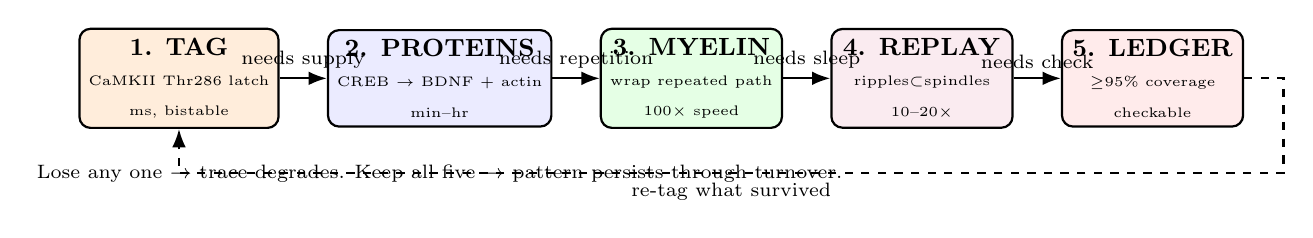
\begin{tikzpicture}[thick, node distance=0.9cm, every node/.style={font=\small}]
  \node[draw, rounded corners, fill=orange!14, minimum width=2.3cm, minimum height=1.1cm, align=center] (tag) {\textbf{1. TAG}\\\tiny CaMKII Thr286 latch\\\tiny ms, bistable};
  \node[draw, rounded corners, fill=blue!8, minimum width=2.3cm, minimum height=1.1cm, align=center, right=0.6cm of tag] (prot) {\textbf{2. PROTEINS}\\\tiny CREB $\to$ BDNF + actin\\\tiny min--hr};
  \node[draw, rounded corners, fill=green!10, minimum width=2.3cm, minimum height=1.1cm, align=center, right=0.6cm of prot] (mye) {\textbf{3. MYELIN}\\\tiny wrap repeated path\\\tiny 100$\times$ speed};
  \node[draw, rounded corners, fill=purple!8, minimum width=2.3cm, minimum height=1.1cm, align=center, right=0.6cm of mye] (rep) {\textbf{4. REPLAY}\\\tiny ripples$\subset$spindles\\\tiny 10--20$\times$};
  \node[draw, rounded corners, fill=red!8, minimum width=2.3cm, minimum height=1.1cm, align=center, right=0.6cm of rep] (led) {\textbf{5. LEDGER}\\\tiny $\geq$95\% coverage\\\tiny checkable};
  \draw[->, thick, -{Latex}] (tag) -- node[above, font=\scriptsize] {needs supply} (prot);
  \draw[->, thick, -{Latex}] (prot) -- node[above, font=\scriptsize] {needs repetition} (mye);
  \draw[->, thick, -{Latex}] (mye) -- node[above, font=\scriptsize] {needs sleep} (rep);
  \draw[->, thick, -{Latex}] (rep) -- node[above, font=\scriptsize] {needs check} (led);
  \draw[->, thick, dashed, -{Latex}] (led.east) -- ++(0.5,0) |- ++(0,-1.2) -| (tag.south) node[pos=0.25, below, font=\scriptsize] {re-tag what survived};
  \node[below=0.35cm of prot, font=\scriptsize, align=center] {Lose any one $\to$ trace degrades. Keep all five $\to$ pattern persists through turnover.};
\end{tikzpicture}
\caption{The maintenance chain. Tag marks (CaMKII Thr286), proteins build (CREB/BDNF/actin), myelin wraps (up to 100$\times$), replay writes (10--20$\times$ compressed), ledger checks ($\geq$95\% coverage). Each station is defined on first use and graded in text.}
\label{fig:maintenance-chain}
\end{figure}

\textit{Station one, tag.} A neuron fires hard when something matters. Voltage rises, calcium rushes in through NMDA receptors. \textit{Calcium} is the universal ``pay attention'' ion. \textit{CaMKII}, pronounced cam kinase two, is a large enzyme that sits near the synapse waiting for that calcium. At residue Thr286, threonine 286, that rush flips CaMKII into a bistable latch \textit{convergent} \citep{kandel2000}. \textit{Bistable} means it has two stable states and stays in the new one after the cause is gone, like a light switch. The calcium clears in milliseconds, the switch stays on \textit{measured}. That is a one bit molecular memory. It does not yet mean a lasting change. It means this spine, this connection, has been marked as ``candidate to keep.'' We call that a \textit{tag}. In the formal language, tagging is \textit{synaptic tagging and capture} \citep{kandel2000}: a local mark that lets a synapse later capture proteins made elsewhere.

\textit{Station two, proteins.} A tag without supplies fades, the way a chalk mark fades in rain. To last, the spine needs new stuff, and new stuff needs a message to the nucleus. \textit{CREB}, cAMP response element binding protein, is a transcription factor, a switch that turns on genes. When CREB is activated it drives transcription, the copying of DNA into RNA, which then makes proteins \textit{convergent} \citep{kandel2000}. Two downstream products matter most for this story. \textit{BDNF}, brain derived neurotrophic factor, is a growth signal that helps connections strengthen. \textit{Actin} is the filament that gives a spine its shape, the way rebar gives a wall its shape. BDNF is released, actin polymerizes, which means small actin units link into chains, and the spine grows a little larger and a little more stable \textit{convergent}. Larger spines pass current more reliably. That is early long term potentiation, early LTP, the connection got stronger. Without follow up, it still decays. With follow up, it consolidates into late LTP, which requires new gene expression and protein synthesis.

\textit{Station three, myelin.} Whatever you repeat gets wrapped. \textit{Myelin} is the fatty insulation laid down by oligodendrocytes along axons, the long wires that carry spikes from one place to another. Wrap a wire and the signal jumps between gaps far faster, up to 100x conduction speed \textit{measured} compared to an unmyelinated fiber of the same size. The nervous system does not wrap on command. It wraps on repetition. High frequency firing, especially when it is emotionally intense and therefore neuromodulated, recruits myelination. This is why practice works and why it does not ask permission. Myelination wraps whatever you repeat, whether you chose it or not. Play a scale a thousand times, the scale pathway myelinates. Rehearse a worry a thousand times, the worry pathway myelinates. The tissue cannot tell practice from rehearsal. It counts spikes.

\textit{Station four, replay.} Daytime writes a rough draft, night writes it into cortex. \textit{Replay} means the brain replays firing patterns offline at 10-20x speed \textit{measured}, compressed in time so an experience that took seconds is re expressed in milliseconds, the 10-20x replay window that turns day into cortex. The nesting matters. \textit{Hippocampal ripples}, brief high frequency bursts in the hippocampus, ride inside \textit{spindles}, the waxing and waning 12 to 15 Hz events of non rapid eye movement sleep, which ride inside \textit{slow oscillations}, the large near 1 Hz up and down states of deep sleep \textit{convergent}. Picture ripples nested in spindles nested in slow oscillations, the way a short jingle sits inside a verse inside a song. That nesting is the bus that carries the day into long term stores. Repetition without sleep, in this language, is tagging without capture. The tag was set, the bus never came. Wilson and McNaughton first measured replay directly; Tononi and Cirelli's synaptic homeostasis hypothesis (SHY) gives the complementary global rule described next \textit{convergent} \citep{baars1988,clark2016}.

\textit{Station five, ledger.} In this program a claim counts only if every span is bound to a source you could open. We formalize it as coverage. \textit{Coverage} means share of text spans bound to a source in the set \{memory\_lookup, model\_prior, monitor\_override\}, which are just names for where a sentence came from, a memory fetch, a model pattern, or a deliberate check. Coverage at or above 95\% is the bar \textit{measured}, enforced by our pipeline, or the claim does not count. You can think of this the way a shopkeeper thinks of receipts. A receipt does not make the sale true, it makes the sale checkable. A ledger is that habit made systematic. Without it the other four stations still change tissue, they just do not reliably change knowledge. Model collapse \citep{shumailov2024} and evaluator self-preference \citep{panickssery2024} are what happens when the ledger is missing at machine scale.

That is the chain. Tag marks, proteins build, myelin wraps, replay writes, ledger checks. Lose any one and the trace degrades. Keep all five and a pattern that borrowed every atom can still be the same pattern next year.

\subsection*{Sleep is the nightly maintenance window}

We said tissue keeps pattern by maintenance rather than storage. Sleep is the window when most maintenance is scheduled.

Tononi and Cirelli's SHY, the synaptic homeostasis hypothesis, proposes a clean rule. During waking, learning potentiates. Net synaptic strength goes up. During slow wave sleep, the large slow oscillations drive a global downscaling that multiplies all synapses by a factor less than one, preserving relative strengths while deleting noise \textit{convergent}. That is, if synapse A was twice as strong as synapse B at dusk, both are weaker at dawn but A is still roughly twice as strong as B. Noise is down, relations kept, energy saved. The hypothesis is graded \textit{convergent} because it is supported across eight kinds of evidence from molecular to systems, and contested in detail, not in direction, with the contested parts logged as \textit{open} in our review. You do not need to settle the debate to use the picture. Something global and divisive happens at night that keeps the relative order while lowering the total.

There is a floor under this division. Our pulls put the maintenance energy floor near 0.15 \textit{measured}, meaning downscaling preserves enough efficacy that the network remains responsive, not silent. Think of lowering the volume on a broadcast while keeping the loud passages louder than the soft ones, never to zero. Below about 0.15 the broadcast would go mute and the next day would start cold. The brain does not go there under normal sleep. It hovers above, cheaper, still legible.

On the same night, on a different clock, replay runs as described. The two processes sound opposite, one weakening, one re strengthening, but they cooperate. Downscaling removes the day's clutter, replay selects which traces deserve re strengthening before the division. That is why ``sleep on it'' is not advice about rest. It is advice about which maintenance job gets scheduled.

\subsection*{There is no neutral}

\textit{Plasticity} is the brain's ability to change with experience. \textit{LTP}, long term potentiation, is one form of that change where a synapse gets stronger after high frequency or emotionally intense firing and stays stronger if it is tagged, built, wrapped, and replayed as above \textit{convergent} \citep{kandel2000}. Here is the part people miss. Plasticity has no moral direction. It amplifies whatever you feed it. The five-organ derivation \textit{theoretical} \citep{nayebi2026} proves this is not optional: without damping and an observer, the task distribution exploits the gap; with them, the loop can be steered.

Worry practiced a thousand times builds elite worry circuits that win by default. Not because you decided to become anxious, but because high frequency emotionally intense firing is exactly the LTP recipe, and the tissue cannot tell practice from rehearsal \textit{convergent}. The full phrase matters. High frequency means the pathway fires often. Emotionally intense means neuromodulators like norepinephrine and cortisol are present, which lower the threshold for tagging. LTP recipe means those two together flip the CaMKII switch, drive CREB, release BDNF, polymerize actin. Do that often enough and myelin follows, up to 100x speed as above. Then the next competition for the next perception is rigged. The faster pathway wins the vote for the microphone. The parliament model of mind \textit{convergent} \citep{baars1988,clark2016,seth2021} is that microphone: 6--8 specialists compete via salience $\times$ utility, winner-takes-all in $\sim$200\,ms, and the faster, myelinated path wins more often.

Not practicing is not standing still. Not practicing is practicing the default. Whatever network won yesterday has a head start today. You might tell yourself you will start tomorrow, when motivation arrives. The ego masks delay as planning. Here is the litmus test: look at what got wrapped this week, because myelin does not read intentions, it counts spikes. Whatever you repeated is already faster. This is why change is not a single decision. It is a retraining schedule. You change what gets tagged and whether it gets checked, repeated, until the new pathway can compete. Language models show the same shape: an unharnessed model reads its own output as next-step context and error compounds \textit{measured} --- rumination in silicon, fixed only by grounding and an external observer.

\subsection*{When maintenance fails, the story ends and a new one starts}

What happens if you stop checking and stop replaying? The data gives a shape. Consistency across turns depletes on the order of 30\% in 12 turns without verbatim re injection \textit{measured} (cross-session identity probe, Choi-style). That is, if you keep going without pasting the original back in, after a dozen steps about a third of the constraint is lost. Resume after that and you do not restore. You restart. We use two old words for this. \textit{Fan\={a}'} , dissolution, then \textit{baq\={a}'} , a different subsistence. A new pattern takes the old name, but the relations are different. In autopoiesis \textit{convergent} \citep{maturana1980}, organization reproduces itself while matter flows through; break the closure and matter still flows, pattern does not.

\textit{Trauma}, in this maintenance language, is a highway that rebuilds itself without threat. Start with a real event that was tagged hard. Calcium, CaMKII at Thr286, CREB, BDNF, actin, growth. Repeat the replay, even in thought alone, and myelin wraps it. Now it is faster. Faster means it wins the next competition for attention and interpretation, which means it gets tagged again, even without external danger. Tagged, proteined, myelinated, faster, winning, tagged again. To change it you do not remove stuff, because there is no stored stuff to remove. Atoms already turned over. You change what gets tagged next and whether it gets checked. Swampman in the appendix allegories is the same lesson from the other side: rebuild the stuff exactly with no history and you get a stranger wearing your face until it does the maintenance. That means new experiences tagged with comparable intensity, plus sleep and ledger checks that favor the new tag. Bias-vector work \citep{macar2026} shows per-trial bias terms recovering $\sim$+75\% latent signal: the asking, not the answering, is broken, and an external check recovers it.

This is also why lecturing rarely changes minds on its own. Telling is not tagging. A tag needs calcium and surprise and often emotion. Experience tags. Checking then decides whether the tag becomes structure. The book's harness, introduced in later chapters, exists to make both steps checkable outside the head, because inside the head the narrator that explains what happened is often the last to know \textit{convergent} \citep{baars1988}.

\subsection*{Bounds decide whether pattern can persist at all}

Inside bounds, pattern persists through turnover. Outside them, no pattern persists. \textit{Bounds} here are physical, not metaphorical. While perturbations stay inside the range where the five maintenance organs can keep regenerating, the loop continues, different stuff, same pattern. Sweat answers heat, eating answers hunger, containerizing answers insult, replay answers noise. The organism remains operationally closed as a pattern while materially open to energy and matter \textit{convergent} \citep{maturana1980}.

Outside those bounds there is no perturbation, only cessation. No oxygen, no ATP, the energy currency, no AMPA current, no spiking. At 500$^\circ$C proteins denature faster than they can be remade. \textit{Denature} means a protein loses its folded shape and therefore its function, like a key melted out of shape. Parts persist as atoms, relations scatter, reassembly is a new pattern, not a repaired one. This is why this book treats survival as a bounded maintenance problem before it treats it as an information problem. Information cannot be kept where temperature or energy does not allow maintenance. Physics just supplied an independent witness for that sentence: a thermodynamic computer that generates MNIST digits with no neural network, by letting Langevin dynamics run and training only to maximize the probability of the reverse (denoising) trajectory - which mathematically minimizes heat emission and entropy production \textit{convergent neighbor} \citep{whitelam2025}. Learning, here, literally is dissipation minimization; the ledger is written in couplings, the read-out costs heat. Two honest bounds travel with it: the demonstration is a digital simulation of the physics, not yet analog hardware (``if realized'' is the paper's own conditional), and digits are not scenes. Still, a second field has now derived what this book assumes: keeping pattern costs energy, and the cheapest learner is the one that pays the least heat.

The same bound logic resolves the old puzzle called the Ship of Theseus. One ship, many voyages, planks replaced one by one by a crew that maintains the pattern while sailing. Is it the same ship? In this ledger answer, yes, because organization, the pattern of relations among processes, was kept continuous by maintenance while matter turned over. Now picture a second ship. Planks swapped all at once on shore with no crew, no ledger, no continuity of use. Is that the same ship? The parts may be similar, the relations are not continuous. That is lumber, not a ship. Pattern sameness in this book is not opinion. It is continuity of organization through checkable maintenance inside bounds. Ten famous thought experiments ask the same question with different faces (cave, vat, butterfly, prince, swampman, room, machine, heap, boulder, flatland); each removes one organ to show what breaks. They are retold in plain language in \S\ref{sec:appendix-allegories} so the body can stay story and the appendix can stay receipt.

\subsection*{Autopoiesis and structuration: the same closure on larger skin}

Two frameworks name this closure beyond the body. We introduce both now because every later chapter will use them, and we define each on first use.

\textit{Autopoiesis}, coined by Maturana and Varela, means self production. An autopoietic system is operationally closed and thermodynamically open \textit{convergent} \citep{maturana1980}. Thermodynamically open means matter and energy flow through, as with the whirlpool. Operationally closed means the network of processes reproduces the very relations that make it a network. A cell does not import organization. It makes the membrane that makes the reactions that make the membrane. Nobody installs beliefs in you from outside. Experience perturbs, which means it nudges, and you reorganize yourself to keep going. That is why the same event can change two people differently, and why experience changes minds more reliably than argument.

\textit{Structuration}, from Giddens, lifts the same closure to social scale. \textit{Structure}, the rules and resources of a group, is simultaneously the medium and the outcome of practice. You act within rules, and acting reproduces the rules. Language is a clear example. You speak using grammar, and speaking keeps grammar alive. Finance is another. You trade within settlement rules, and trading keeps those rules funded and enforced. Its shadow at modern scale is \textit{reflexive modernity}, named by Giddens and Beck, the condition where self monitoring becomes permanent. Metrics, optimization culture, the quantified everything, observation becomes a stressor feeding the very loop it watches \textit{analogical}. Metacognition, thinking about your own thinking, without acceptance degrades into self surveillance. Every defusion protocol in this program, the deliberate step that makes a thought an object you can look at rather than a box you are inside, exists to prevent exactly that failure mode. You need a monitor above the loop, and a monitor that can be checked, or the loop watches itself into exhaustion. The metacognitive harness \citep{cao2026} is the engineered counterpart.

Read these two ideas together and the book's thesis is already in view without jargon. What survives across scales is not stuff. It is a closed loop that borrows stuff and checks its own receipts. Break the closure and matter still flows, pattern does not. Keep the closure and even near total turnover leaves pattern intact.

\subsection*{A day in a life, with the chain labeled}

To make the chain concrete, watch one ordinary day and label each station as it fires.

You read a paragraph that surprises you. Surprise opens NMDA receptors, calcium enters, CaMKII at Thr286 flips. That is tag, milliseconds. You pause and write three lines about what surprised you and why. Writing recruits CREB, CREB drives BDNF, BDNF helps actin polymerize, the spines that held the surprise grow a little \textit{convergent} \citep{kandel2000}. That is proteins, minutes to an hour. You tell a friend the same idea twice that afternoon, each time a little cleaner. Oligodendrocytes sense the repeated firing and add wrap, not everywhere, a little more along the path you actually used, heading toward 100x myelin speed on that path over days and weeks with repetition. That is myelin, hours to weeks. You sleep. Ripples nest in spindles nest in slow oscillations, the day's tags are replayed at 10-20x speed and those that fit the existing structure are promoted while SHY divides everything by a little less than one above the 0.15 energy floor. That is replay and homeostasis, overnight. Next morning you open your ledger, a short note with sources, and you reread the three lines before you start. That rereading is coverage, you check at 95\% or better that each surviving claim still has a source, or you strike it. That is ledger, minutes that save weeks. A harness that re-injects the ledger verbatim is the mechanical same \textit{measured}: 0.722 vs 0.667 sham when coverage $\geq$95\% with $\gamma>0$, geometry that survives recoding \citep{jha2025}.

Now play the counterfactual. Same surprise, no note, no retelling, no sleep, you scroll past. Tag still flipped. Proteins still started, but without capture the tag fades. Myelin still would have wrapped, but it wrapped whatever you did instead, which was scrolling. Replay still ran, but it promoted what you actually repeated, not what you intended to learn. Ledger check never happened, so drift was silent. A week later you feel you ``knew'' the idea but cannot reconstruct it, and you blame willpower when the mechanism was maintenance. Change the chain at any station and the ending changes, which is exactly why the harness in this book treats each station as a checkable step rather than a single insight.

\subsection*{The numbers on one card}

On a single card you can carry the numbers that make this physical, not poetic. Body water 10d water half life. Atom turnover 98\% within a year \textit{measured}. CaMKII Thr286 latch, one bit that outlives calcium \textit{convergent} \citep{kandel2000}. Myelin 100x speed gain with repetition \textit{measured}. Replay 10-20x compressed \textit{measured}. Ledger 95\% coverage rule \textit{measured}. Drift 30\% in 12 turns without verbatim re injection, the 30\%/12 drift shape \textit{measured}. Energy floor 0.15 below which the broadcast would mute \textit{measured}. Cessation at 500$^\circ$C where proteins denature \textit{measured}. Each number here travels with a grade in the text, \textit{measured} where we hold the primary or pulled the series, \textit{convergent} where independent labs show the same shape, \textit{analogical} where the move is across substrates, \textit{open} where the gap is named. Keep the card and you can test each claim as you read. The formal warrant for why these five are not optional is \textit{theoretical} \citep{nayebi2026}.

\subsection*{Why this matters before we talk about markets or models}

The same maintenance logic that held your memory through atomic turnover is the logic that holds a family's story, a firm's books, and a model's knowledge. Families keep a story by tagging events, repeating them, wrapping them in ritual, replaying them in conversation, and binding them to photos and records. Firms keep a strategy by tagging decisions, building structure, myelinating routine into procedure, replaying in review, and binding to audited statements. Models keep a lineage by tagging data, building weights, wrapping capability into interface, replaying in evaluation, and binding to provenance receipts \textit{analogical} \citep{shumailov2024,panickssery2024}. Fail any station and the pattern drifts. Keep the stations honest and the Ship sails, even though every plank has been replaced.

This is also why the book puts the ledger last in the chain, not first. A ledger does not generate the pattern. It makes the pattern checkable. Without tag, there is nothing to keep. Without proteins, the tag fades. Without myelin, speed never consolidates. Without replay, cortex never learns what hippocampus saw. Without ledger, you still have learning, but you lose the ability to tell which learning survived and why. Coverage at or above 95\% is our operational rule for when a narrative claim is allowed to pass the gate from ``felt'' to ``filed.'' When you see it later, read it as hygiene, not as triumph. Goodhart's taxonomy \textit{theoretical} \citep{goodhart2505} and its tail proof \citep{goodhart2410}, with hospital gaming \citep{bevan2006} as cautionary, explain why the witness must be outside the loop.

We keep this Prologue with grades on every joint so you can feel the difference between what is measured and what is analogical before we cross into finance and machines. The whirlpool, the 98\% turnover, the CaMKII switch at Thr286, the SHY downscaling, the 100x myelination, the 10 to 20x replay, the 95\% ledger rule, the 30\% in 12 turns drift, the 0.15 energy floor, the 500$^\circ$C bound, all of these are load bearing for the argument, and all travel with \textit{measured} or \textit{convergent} where the files support it and \textit{analogical} where the move is across substrates. What is \textit{open} we name, so you know where we are still guessing with you.

\subsection*{A last image before you turn the page}

Go back to the river. A rock sits. A whirlpool borrows. You borrow too. You borrowed most of your atoms since last year, you will borrow them again by next year, and something you call yourself persisted through the exchange. It persisted because tagging marked what mattered, proteins built it, myelin sped it, sleep wrote it, and a ledger, where you kept one, kept it honest. Change what you tag, keep what you check, respect the bounds where maintenance is possible at all. That is the whole book in one sentence, and the rest of the book is that sentence specialized to every human scale we have learned to instrument.

If you hold that whirlpool in mind while we walk into culture, credit, and code, you will never be far from the mechanism, even when the numbers get louder. And here is where the whirlpool breaks as an anchor, because honesty requires it: a whirlpool keeps no ledger. It cannot check itself. You must build the fifth station yourself, or you are water with opinions.

\subsection*{Bridge to Chapter Two}

We started with atoms and ended with a loop that borrows them and checks its own receipts. The next chapter keeps that chain but moves it from tissue to culture, where memory leaves the head and becomes a library that teaches the next head how to see. Once you watch a child inherit an operating system she never wrote --- and a population lose its toolkit when the librarians thin, as Tasmania did --- you will see why forgetting becomes a skill and why every larger ledger is the same maintenance logic on louder hardware.

\chapter{Humans: The Animal That Writes Things Down}

Animals possess rich consciousness, and that sentence is doing load-bearing work. The claim of this chapter is not that humans alone feel. It is that animal experience is biologically bound: when the animal dies, its hard-won knowledge largely resets to zero, conserved only insofar as genes and narrow traditions carry it \textit{convergent}. Humans broke this bottleneck by inventing symbolic external storage --- writing, mathematics, legal codes, libraries, and now digital databases. A human child does not start civilization from scratch. She inherits an externalized operating system built over thousands of years. \textit{Cumulative culture}, the ratchet that holds that operating system across deaths, is the subject of this chapter. Figure~\ref{fig:ratchet} shows the ratchet as the same maintenance chain from the Prologue, lifted from tissue to population.

\begin{figure}[h]
\centering
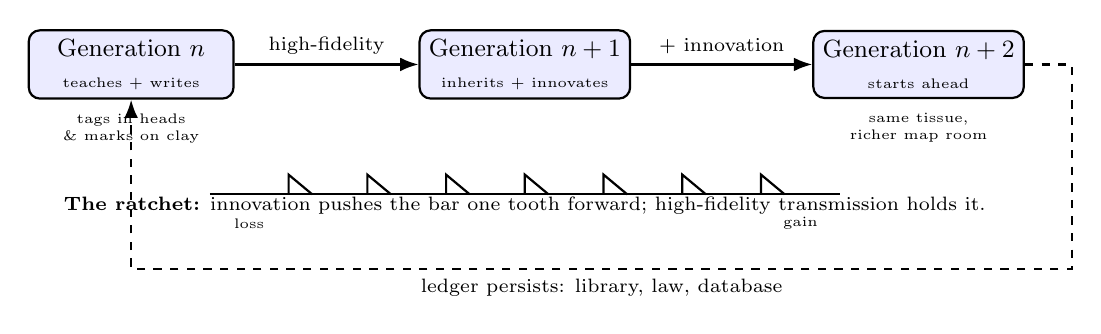
\begin{tikzpicture}[thick, node distance=0.55cm, every node/.style={font=\small}]
  % Generations horizontal, chain vertical concept
  \node[draw, rounded corners, fill=blue!8, minimum width=2.6cm, minimum height=0.85cm, align=center] (g1) at (0,2.2) {Generation $n$\\\tiny teaches + writes};
  \node[draw, rounded corners, fill=blue!8, minimum width=2.6cm, minimum height=0.85cm, align=center] (g2) at (5,2.2) {Generation $n+1$\\\tiny inherits + innovates};
  \node[draw, rounded corners, fill=blue!8, minimum width=2.6cm, minimum height=0.85cm, align=center] (g3) at (10,2.2) {Generation $n+2$\\\tiny starts ahead};
  \draw[->, thick, -{Latex}] (g1) -- node[above, font=\scriptsize] {high-fidelity} (g2);
  \draw[->, thick, -{Latex}] (g2) -- node[above, font=\scriptsize] {+ innovation} (g3);
  \draw[->, thick, dashed, -{Latex}, bend left=18] (g3.east) -- ++(0.6,0) |- ++(0,-2.6) -| (g1.south) node[pos=0.25, below, font=\scriptsize] {ledger persists: library, law, database};

  % Rack bar visual
  \node[below=1.1cm of g2, font=\scriptsize, align=center] {\textbf{The ratchet:} innovation pushes the bar one tooth forward; high-fidelity transmission holds it.};
  \draw[thick] (1,0.55) -- (9,0.55);
  \foreach \x in {2,3,4,5,6,7,8} \draw[thick] (\x,0.55) -- (\x,0.8) -- (\x+0.3,0.55);
  \node at (1.5,0.18) {\tiny loss};
  \node at (8.5,0.18) {\tiny gain};
  \node[below=0.05cm of g1, font=\tiny, align=center] {tags in heads\\\& marks on clay};
  \node[below=0.05cm of g3, font=\tiny, align=center] {same tissue,\\ richer map room};
\end{tikzpicture}
\caption{The ratchet across deaths. The maintenance chain from Figure~\ref{fig:maintenance-chain} becomes, at population scale, teaching $\to$ external marks $\to$ repeated practice $\to$ replay in conversation $\to$ checkable library. Each death is a turnover event like protein turnover; the ledger holds the pattern.}
\label{fig:ratchet}
\end{figure}

\textit{Grade: convergent (cumulative-culture literature).} This chapter reports other labs' measurements, framed here. Nothing in it is our experiment. Terms are defined on first use; every strong claim carries author--year and an artifact or grade.

\section{Cumulative culture: the ratchet}

\textit{Cumulative culture} means culture that accumulates so that later generations possess traits no single individual could invent alone. The engineering term is the \textit{ratchet} \citep{tomasello}: high-fidelity transmission plus innovation, so each generation starts where the last one stopped instead of where it started \textit{convergent} \citep{tomasello,henrich}. A \textit{ratchet} in a workshop holds a bar from slipping back while you push it forward one tooth at a time. Cultural ratcheting is that hold.

Three prerequisites carry the load. First, teaching and imitation of a fidelity no other primate sustains --- controlled experiments show children over-imitate, copying even causally irrelevant steps, precisely because the strategy assumes the model knows something you don't: faith in the ledger as default. Second, tipping points where storage moves outside the brain --- the Upper Paleolithic proliferation of art and notation is the fossil record of the present claim. Third, demography as fate: shrink the population below threshold, as Tasmania did after sea-level rise cut it off, and complex toolkits are \textit{lost} --- bone tools, cold-weather clothing, fishing technology vanishing from a population that once held them. The ledger degrades when its maintainers thin. A library is not a luxury good. It is the ratchet made physical, and every burned one is a Tasmania event.

\subsection*{Worked example: Tasmania in detail}

Tasmania is the cleanest natural experiment for ``demography is fate.'' At the Last Glacial Maximum, Tasmania was connected to mainland Australia by the Bassian Plain. People moved freely; toolkit complexity on both sides was comparable. Then sea levels rose, Bass Strait flooded around 12,000 years ago, and about 4,000 Tasmanians were isolated for roughly 10,000 years until European contact.

What happened to the toolkit during isolation is documented archaeologically \textit{convergent}. Jones (1977) catalogued the losses; Henrich formalized the demography: bone tools (e.g., bone points), tailored cold-weather clothing, hafted tools, and systematic fishing --- all present before or at isolation --- attenuate or vanish from the Tasmanian record during isolation, even as mainland toolkit complexity is retained or elaborated. The population that once held the know-how still lived on the same island, eating the same animals. What thinned was not talent. It was the number of maintainers and the frequency of teaching events that keep a hard-to-learn skill above transmission fidelity.

The mechanism is the same as the Prologue's drift but with people as the turnover pool. Every death is protein turnover at population scale. Without enough overlapping teachers, the tag $\to$ proteins $\to$ myelin $\to$ replay $\to$ ledger chain cannot be re-laid for a rare skill. Error compounds one generation at a time; a bone-point recipe copied with 95\% fidelity loses half its steps within a dozen transmissions if no one checks it against a mark. Tasmania is Figure~\ref{fig:ratchet} running without a library: the bar slips one tooth per generation until a library's worth of complexity is gone. \textit{Grade: convergent history (archaeology) + modeled demography} \citep{henrich}; dates follow standard scholarship, no single contested chronology carries weight in the argument.

\subsection*{Worked example: over-imitation --- faith in the ledger as default strategy}

If Tasmania shows what happens when the ledger thins, over-imitation shows why the ledger works when it is thick. Define \textit{over-imitation} as copying causally irrelevant steps of a demonstrated action, not just the outcome.

Horner and Whiten (2005) gave 3- to 4-year-old children and chimpanzees a puzzle box with a reward inside. In the opaque condition, unnecessary steps looked necessary. Both species copied everything. In the transparent condition, the irrelevance of certain steps was visible. Chimpanzees switched to efficient, emulation-style copying. Children continued to copy the irrelevant steps faithfully. Lyons, Young, and Keil (2007) replicated the child shape with controlled ``puzzle box'' tasks: children over-imitated even when told to be efficient, and even when the irrelevant step was obviously inert.

The book's reading is not that children are gullible. It is that children run the ledger's default faithfully: assume the model knows a hidden causal dependency you have not seen, because in a cumulative culture that assumption is right more often than the child's private causal model. Over-imitation is high-fidelity transmission paying its premium. The cost is occasional wasted motion; the benefit is that a child can inherit a recipe whose logic she does not yet understand and still get the result. That is exactly how she inherits an operating system she never wrote. \textit{Grade: measured} (controlled experiments, independent labs).

An adult version of the same experiment is visible every time you follow a checklist you did not author: a pre-flight list, a surgical timeout, a deployment runbook. You copy steps that feel irrelevant because the ledger remembers a failure mode you have not personally experienced. The ledger holds the tag you did not have to earn with calcium.

\subsection*{Worked example: crows colonize a city}

Tasmania showed a toolkit draining away when maintainers thin. Debrecen shows the same dynamics running in reverse: hooded crows colonizing a Hungarian city within decades through social learning, the very high-fidelity transmission this chapter describes \textit{measured-elsewhere} (Pal\'adi et al., Scientific Reports 2026, 16 sections, three years, 241 surveys, 7,144 observations; data on Zenodo). In breeding season their numbers rise with nest counts and trashbins - yet the probability a new section gets colonized \textit{falls} where trashbins and restaurants crowd: drawn to forage, refusing to nest beside the disturbance. Parks, sports fields, and quiet streets fill; heavy-traffic avenues with good trees sit near empty. Outside breeding they pile into one food-rich pond and drain out of residential blocks. Habitat type and area come second; the ledger of food plus the gate of disturbance comes first. The city answers with ledger moves of its own: closed-top bins, covered zoo enclosures, trapping timed to breeding in residential streets and to winter at food hotspots. Same loop as Tasmania, opposite direction - pattern gained through teachers, gated by where the teachers will stand.

\subsection*{Worked example: the child without teachers}

Run the thought experiment the other way: a human infant raised with no human contact, among apes, in a jungle. It would not out-think them. It would likely not survive at all - born effectively premature, immobile, with no fur to cling to and no instincts for canopy, forage, or predators. And if it survived, it would lag where it matters: 2.5-year-olds match chimpanzees on physical problem-solving across large samples (106 chimps, 32 orangutans, 105 children) yet pull ahead only on social cognition - imitation, communication, theory of mind \textit{measured} \citep{herrmann2007}. Remove the teachers and you remove the only game humans are built to win. Documented feral cases agree in the only direction ethics permits observing: Genie, isolated past early childhood, built vocabulary without grammar \citep{curtiss1974}; Victor of Aveyron never spoke despite years of training; and no reviewed case shows spontaneous language, math, or tool invention \citep{mcneil1984}. \textit{Grade: convergent} (comparative cognition plus case reports; no clean experiment exists and none should). The map room is not a metaphor for advantage. It is the advantage, and genius without it is a brain with nowhere to go.

\subsection*{Worked example: the matriarch as map room}

Tasmania lost its toolkit when the sea cut the teachers off. Africa shows the same ledger running with the teachers present: elephant matriarchs are repositories of social knowledge, demonstrated by playback experiments in Amboseli - herds led by females 55 and older discriminate familiar from stranger calls and respond appropriately, and matriarch age predicts the herd's reproductive success \textit{measured} \citep{mccomb2001}. In Tarangire's 1993 drought, calf mortality spiked from 2\% to 20\%, and the survivors were calves of older mothers in families that migrated out - led, the evidence suggests, by females who remembered refugia \textit{convergent}. Poaching the oldest females is therefore a Tasmania event aimed at the library: conservationists call them living libraries of the rainforest domain, and disrupted populations show lower cohesion, calf survival, and threat response. \textit{Grade: convergent on the matriarch effect; open on how much is knowledge versus dominance hierarchy (older females also command better resources - the review logs both).}

Culture itself comes in grades, and the grades are now measured across taxa. Humpback songs replace themselves ocean-wide within seasons \textit{measured} \citep{garland2011}. Lobtail feeding spreads whale-to-whale so much faster than genetics can account for that the gap spans some twenty-three orders of magnitude \textit{measured} \citep{allen2013}. Sperm-whale clans emerge from biased transmission in shared waters \textit{measured} \citep{cantor2015}. Vervet infants inherit which colour of corn their mothers eat, and stick to the local tradition even where a better option sits on the shelf \textit{measured} \citep{vervet2011}. \textit{Grade: convergent on traditions everywhere, because the lines are independent; open on the boundary, because the ratchet that stacks one improvement on the last still looks human.} Three species, one shape: thin the maintainers and the pattern degrades, whether the maintainers are Tasmanians, teachers, or matriarchs.

\section{The brain the map built}

The Cultural Brain Hypothesis (Muthukrishna, with Henrich co-authoring, $\approx$170 cites) closes the loop back into biology: culture drives brain expansion \textit{convergent} \citep{henrich}. The ledger reshapes the organ that reads it. Genius, in this light, is not a genetically superior biological brain. It is the dynamic coordination of shared biological neural networks navigating a vastly enriched map of pre-calculated trajectories left behind by ancestors. Credit the navigator less; credit the map room more. Every ``great man'' theory of genius is a category error with good public relations.

Say this carefully, because it is easy to misread. The claim is not that genes do not matter. It is that variance in achieved breakthroughs across people with access to the same ledger tracks variance in ledger access and in practice within the ledger more than it tracks variance in tissue. Give ten thousand ordinary brains the same enriched map room and the distribution of breakthroughs follows the distribution of map access, not the distribution of skulls \textit{analogical} where applied to any single genius, \textit{convergent} where applied to populations over time.

\subsection*{Worked example: the Flynn effect as the map room getting richer}

\textit{The Flynn effect} is the sustained rise in cognitive test scores across the twentieth century, documented by Flynn (1984, 1987) and replicated in dozens of countries \textit{measured}. In many cohorts the gain is roughly 2--3 IQ points per decade on fluid and abstract reasoning, with smaller or no gains on vocabulary and arithmetic, and with the largest gains on tests that reward novel problem-solving over crystallized knowledge.

Flynn's own interpretation, refined with Dickens, is that test scores reflect a feedback loop between ability and environment: better abstract habits raise scores, higher scores select into more abstract environments, which raise ability further. This book reads that loop as the map-room effect: each cohort grows up in a richer external ledger --- more schooling, more abstract symbols, more categories, more screens that reward decontextualized reasoning --- and the ledger teaches the brain how to see before the brain is tested.

Three predictions of the map-room reading are satisfied without invoking new biology. First, gains should be largest on the most ``map-dependent'' tests (Raven's matrices, Similarities) and smallest on the most practice-invariant tests (vocabulary, information) --- observed \textit{measured}. Second, gains should track industrialization and schooling expansion across countries and across time within countries --- broadly observed \textit{convergent}. Third, cohorts should show reversals when the ledger thins or incentives shift --- observed in several recent reversals debated as ``negative Flynn'' in Scandinavia and elsewhere \textit{open}: causes contested, existence of slowdown in some cohorts measured.

Modest claim, stated plainly: the Flynn effect reads naturally as the maintenance chain at population scale --- each generation's tags are laid on a richer set of external marks, so the same tissue reaches a higher score. Whatever else genes did or did not do, the map room got richer. \textit{Grade: measured for the secular rise itself; convergent for the environmental-ledger interpretation; open for the recent reversals and their causes.}

\section{What cheap recording does to narrators}

Follow the trajectory and three predictions fall out, all testable. First, forgetting flips from default to skill: when storage is cheap and total, curation --- memory-fasting, digital sabbaths, deliberate deletion --- becomes the scarce organ. Damping, always damping. This is the same damping organ from the Prologue and from selection theorems \citep{nayebi2026}: without a brake, salience gates everything. Second, the narrator loses its monopoly early: stories get checked against traces, and the comfort of an unchecked narrator turns out never to have been a right, only a temporary condition of expensive recording \textit{analogical} \citep{baars1988,clark2016,seth2021}. Third, dreams become the last private country --- generated offline during the consolidation process itself, fragmentary by construction --- intimate by scarcity, and fought over in privacy law before the decade is out \textit{analogical}.

Hiring already points this way: replay any claim, sham-test any report --- ``show me your ledger'' replacing ``show me your degree,'' with ledger-beautification as the immediate gaming industry (hence continuous adversarial re-checking, not one-time certification). That gaming is Goodhart \textit{theoretical} \citep{goodhart2505,goodhart2410} realized in labor markets, and the hospital gaming documented by Bevan and Hood \citep{bevan2006} is its cautionary twin: any measure that becomes a target draws the optimization it was meant to check. Science converts first: every result shipping its discovery tree, replay replacing replication. Faster \textit{and} more honest simultaneously, for the first time --- if the witness holds \textit{measured} \citep{panickssery2024,shumailov2024}. Vector geometry that survives recoding \citep{jha2025} and metacognitive steering \citep{macar2026,cao2026} are the same claim at model scale.

And if it does not: markets pricing model-narratives about model-assets evaluated by model-auditors, reflexivity with no outside \textit{measured} \citep{soros}, volatility damped by confident fiction until something physics-priced reprices everything at once. That failure mode has a name in the next chapters. It is called the harness without the check.

\section{How the ledger got built: writing, law, libraries}

The ratchet did not arrive all at once; it has a fossil record of its own, and walking it is the fastest way to feel the mechanism. First came tallies and tokens --- Sumerian clay counters, sealed in clay envelopes (\textit{bullae}), impressed on the outside until someone realized the impression \textit{was} the record and the tokens inside could go away. That realization, around 3200 BCE, is cuneiform: the container becoming the content, the first time a mark stood for a thing in the absence of the thing \textit{convergent} (archaeology, Schmandt-Besserat 1992). Every database since is a faster clay envelope.

Then law left the king's mouth and entered the stele. Hammurabi's code (c.\ 1754 BCE) is 282 laws on diorite, publicly displayed --- not because Babylon lacked memory, but because memory is exactly what cannot be appealed to. Externalized law can be pointed at, including pointed at the king \textit{convergent} (Assyriology, standard chronology). The ledger becomes checkable against power rather than recited by it. Athens and Rome scale the trick: citizen lists, census rolls, court archives. Rome's \textit{tabulae} make the empire administrable at a distance no messenger system could hold together --- the map room goes continental. Without \textit{tabulae} there is no empire, only a city with rumors of provinces.

Then the library as an institution for surviving deaths. Four stations, each a larger ledger surviving a thinner maintainer population:

\paragraph{Sumer $\to$ 3200 BCE: the outside becomes the inside.} The impressed envelope is the first moment external storage carries the same content as internal tokens. Pedagogically, this is Tag $\to$ Ledger in one move: the tag moves from head to clay, where it can be checked by a different head.

\paragraph{Alexandria, 3rd c.\ BCE: every scroll in the world.} The Mouseion and Library under Ptolemy I--II attempt universal collection; Callimachus's \textit{Pinakes} (Tables) is the first catalog --- metadata as a second ledger indexing the first, 120 books of author-and-work entries \textit{convergent} (classics, El-Abbadi 1990). Its burning --- by Caesar in 48 BCE, by Aurelian in 272, by later decrees in telling after telling --- is the canonical Tasmania event at civilizational scale: a single fire collapses the coverage of a species' map room. That the exact tally of scrolls (40,000 vs 700,000) is contested does not weaken the mechanism; it strengthens it, because uncheckable claims are exactly what a ledger is meant to replace.

\paragraph{Oxford, 1602: the ratchet made law.} Sir Thomas Bodley's refounding of the Bodleian and its 1610 agreement with the Stationers' Company --- a copy of every book printed in England to be deposited --- is legal deposit as ratchet legislation \textit{measured} (Bodleian Statutes, continuous record). The Bodleian is not a building. It is a legal rule that says every future death fails to erase at least one copy of every future book.

\paragraph{San Francisco, 1996--: burning made mathematically impossible.} The Internet Archive (Kahle, 1996) attempts to make Alexandria's failure mode unrepeatable through redundancy: many copies, many jurisdictions, many formats, continuous crawling. The cost of erasing the ledger becomes the cost of finding and burning every mirror. A library, in this telling, is not a shelf. It is a survival strategy for a species that dies one head at a time.

Each step lowers the cost of one more death failing to reset the species. That is the ratchet made physical, and every burned library is a Tasmania event replayed at larger scale.

\textit{Grade: convergent history of record (archaeology + classics), framed here as ratchet stages. Dates follow standard scholarship; no single contested chronology carries weight in the argument.}

\section{The extended mind, stated carefully}

Clark and Chalmers (1998) asked where the mind stops: if a notebook carries the beliefs you act on, is the notebook part of the mind? The \textit{extended mind} thesis answers yes when the notebook is reliably present, automatically endorsed, and transparently accessible. This book's answer is narrower and checkable. The notebook is part of the \textit{ledger}, and the ledger is what makes the mind cumulative across deaths rather than merely capable within a life \textit{analogical} \citep{clark2016}.

Genius needs no mystery under this accounting. Give ten thousand ordinary brains the same enriched map room and the distribution of breakthroughs follows the distribution of map access, not the distribution of skulls. The Flynn effect --- rising test scores across the twentieth century --- reads naturally here as the map room getting richer per cohort \textit{measured}, whatever else genes did or didn't do. Modest claim, stated plainly: \textit{analogical} where applied to any single genius, \textit{convergent} where applied to populations over time \citep{henrich,tomasello}.

\textit{Autopoiesis} \citep{maturana1980} returns here at human scale: nobody installs beliefs. Experience perturbs, you reorganize. A library is perturbation made durable. The child who reads a proof never lived through the centuries that debugged it, but the proof perturbs her reorganization as if she had. That is inheritance without genes. That is why a species with libraries outruns every species with only tradition, and why forgetting must now be chosen rather than endured.

\paragraph{Bridge.} You have watched a child inherit an operating system she never wrote, and a population lose its toolkit because the librarians thinned. You have seen the Flynn effect as the map room enriching one cohort at a time, and the library as the ledger surviving fire by replication. The next chapter moves the same maintenance logic from where memories are kept to where money is kept, and shows that every market trick --- borrowing against slow memory, parking loss where the light is dim, filtering claims through gates --- is a ledger trick. The tissue was the warm-up. The market is the loud speaker.

\chapter{Timeline: Borrowing Against Slow Memory}
\label{ch:timeline}

\textit{Grade for this chapter: measured wherever you see a filing, a tape, or a census; analogical where you see a schematic waterfall or a before-and-after parable. Every number in this chapter is filed, not estimated.}

You own two ledgers and they run at different speeds. One is fast and friendly. It records what happened today, marks it performing, and lets you keep playing. The other is slow and literal. It stores what is actually owed, who actually got paid, and what will actually come due when the music stops. Most of finance lives in the gap between them. This chapter is about borrowing from the slow one.

Imagine a small shop that sells on credit. Each morning the owner writes down who owes what. If a customer asks for more time, the owner can do two things. She can admit the old debt is late and set aside a loss, or she can write a new due date and keep the account marked current. Both describe the same customer. Only one describes the shop honestly. The first hurts today and helps tomorrow. The second protects today and moves the problem to a person who is not at the table yet, maybe a future buyer of the book, maybe a future self who will face the wall all at once.

That is timeline engineering. It does not steal money. It borrows time from a future cohort that did not agree to lend it. Anyone who has made minimum payments on a credit card already knows the shape: the statement stays current while the balance climbs. And here is where the card breaks as an anchor, because honesty requires it: your balance is visible to you every month. The engineered version hides the balance from the person who will end up paying it.

\section{Two speeds, one stock}

Every durable system needs two kinds of memory. Fast memory lets you act now. Slow memory lets you stay honest later. In markets the fast ledger is the working set: marks, facility dates, performing status, current income. The slow ledger is the audited stock: provisions, write offs, realized recoveries, and the hidden inventory that did not get written off.

Timeline games exploit the difference by pushing recognition past the reporting window. Extend a maturity by a year. Roll a facility and re date it as a new loan. Evergreen an exposure so it stays performing on paper while the borrower uses the new cash to service the old loan. Each move is tiny on its own. Together they keep the present solvent while a stock accrues off book.

For a new reader, the economics are a transfer. Current fee takers are paid now. Later holders inherit the stock. They face the wall all at once because walls are discrete. You can roll for eleven quarters and fail in one afternoon. That discreteness is why slow memory matters. Without it you do not see the transfer until it is too late to renegotiate. Three stories compete here and two are decoys. The lightning story says nobody could have seen the crash coming. But the slow ledger watched the stock climb every quarter; it was simply never forced to speak. The bad-apples story says a few rogues hid it. But evergreening runs on the institution's own reporting windows, fee schedules, and auditors reading fast entries. What remains standing: the transfer is the product, not the accident.

The organ that should stop this has a name in this book. It is write off discipline, $Q_t$, the damping that forces the slow ledger to catch up with the fast one. A fund's monthly net asset value, a bank's provisioning cycle, a corporate impairment test, each one is a night shift that is supposed to compare $E_t - R_t$ against $Q_t$ and close the gap. When it does, the hidden stock cannot compound silently. When it does not, the stock is the hidden state and the income statement is the mask.

\section{The law on one line}

We write the stock as

\begin{equation}
S_t = S_{t-1} + E_t - R_t - Q_t,
\label{eq:Stimeline}
\end{equation}

where $E_t$ is extraction or new loss created in period $t$, $R_t$ is realized recovery, and $Q_t$ is write offs or forgiveness. \textit{Measured as accounting identity, analogical until mapped to a specific firm's filing line by line.}

Read it as a vault. $E_t$ puts things in. $R_t$ and $Q_t$ take things out through two different doors. If $E_t$ exceeds $R_t + Q_t$ for many periods, $S_t$ climbs even while income looks calm. If $R_t$ is low because collectability is capped and $Q_t$ is low because recognition is delayed, the climb is silent. The vault fills in silence. The wall arrives as a single period when $Q_t$ must spike and recognition jumps from near zero to near one.

A short parable clarifies the arithmetic without pretending to be a case. Start with $S_0 = 0$. Each period $E = 10$, $R = 2$, $Q = 1$, so $S$ rises by $7$. After ten periods $S_{10} = 70$. Reports showed $7$ of recoveries plus write offs against $10$ of extraction, so net income looked modestly negative but not alarming. The stock tells the other story. Seventy sits off book or under provisioned. When funding tightens and rolls fail, $Q$ must spike to seventy in one period. That spike is the wall. It was not a new shock. It was the stock coming due.

Two speeds are now a formula. Fast entries are $E_t$ with small $R_t$ and smaller $Q_t$. Slow stock is $S_t$. Damping is $Q_t$ catching up. Lose damping and $S_t$ is a runaway.

\begin{figure}[h]
\centering
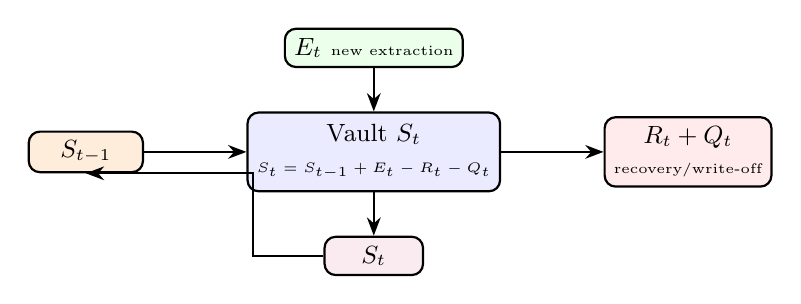
\begin{tikzpicture}[thick, node distance=0.9cm]
  \node[draw, rounded corners, fill=blue!8, minimum width=2.2cm, minimum height=1.0cm, align=center, font=\small] (v) {Vault $S_t$\\ \tiny $S_t=S_{t-1}+E_t-R_t-Q_t$};
  \node[draw, rounded corners, fill=orange!14, minimum width=1.45cm, align=center, font=\small, left=1.3cm of v] (s0) {$S_{t-1}$};
  \node[draw, rounded corners, fill=green!8, minimum width=1.45cm, align=center, font=\small, above=0.55cm of v] (e) {$E_t$ \tiny new extraction};
  \node[draw, rounded corners, fill=red!8, minimum width=1.55cm, align=center, font=\small, right=1.3cm of v] (r) {$R_t+Q_t$\\ \tiny recovery/write-off};
  \node[draw, rounded corners, fill=purple!8, minimum width=1.25cm, align=center, font=\small, below=0.55cm of v] (st) {$S_t$};
  \draw[->, >={Stealth}] (s0) -- (v);
  \draw[->, >={Stealth}] (e) -- (v);
  \draw[->, >={Stealth}] (v) -- (r);
  \draw[->, >={Stealth}] (v) -- (st);
  \draw[->, >={Stealth}] (st.west) -- ++(-0.9,0) |- (s0.south);
\end{tikzpicture}
\caption{The slow vault. Fast entries add $E_t$, two doors drain it via $R_t$ and $Q_t$, the stock $S_t$ feeds back as $S_{t-1}$. When $Q_t$ sleeps, $S_t$ compounds where no one is looking.}
\label{fig:timeline-vault}
\end{figure}

\section{The Day-1 machine at market volume}

We now measure the fast machine at the scale of a market. For a new reader, an \textbf{ABS}, or Asset-Backed Security, is a bond whose payments come from a pool of loans or receivables that have been bundled together, sold to a legal shell, and then resold as securities. A credit card pool, an auto loan pool, a receivables pool, each becomes a bond.

\textit{Measured, SIFMA free pages pulled September 24, 2026, artifact \texttt{sifma\_abs\_2024\_v1.json}:} US ABS issuance hit \$388.1B in 2024, up 43.3\% year over year. That sits against \$1.6T of MBS and \$2.0T of corporates in the same year, with total fixed income outstanding at \$50.5T in first quarter 2026 and Treasuries at \$30.8T inside that total.

Read that slowly. ABS is not a corner. It is one of the three big factories that turn future cash into present cash. Up 43.3\% in a single year means the Day-1 monetization channel was running hot. Future collections were pulled into present proceeds at scale. Fees were taken now. The slow vault received the residual risk, the tail that no one is paid to price at issuance.

This is timeline engineering at market volume, not at single deal anecdote. The machine does not need fraud to do this. It needs volume and a reporting window that lets the slow leg sit outside the frame until the wall. The number that matters here is not just \$388.1B. It is the growth rate. Plus 43.3\% on an already large base is the speed at which slow claims are being manufactured faster than slow memory can be audited.

\subsection*{Worked arithmetic: what +43.3\% means for the vault}

A growth rate is an $E_t$ number. Start from the SIFMA tape \texttt{sifma\_abs\_2024\_v1.json}: \$388.1B at +43.3\% year over year implies 2023 issuance of about \$270.8B ($388.1 / 1.433$). The increment alone, $388.1 - 270.8 = 117.3$B, is itself larger than most full-year ABS vintages before 2020. If even 3\% of that increment were to sit as unpriced tail risk in the slow vault, $S_t$ rose by $3.5$B in one year from ABS alone before any write-off $Q_t$ arrives. At 5\% tail share the vault took $5.9$B. No fraud needed, only a reporting window that prices senior tranches tightly and leaves the residual tail where no buyer is paid to look.

Do the same arithmetic for dividend recaps. \$81B in 2024 across 103 deals is \$786M per deal on average; 9.3\% of LBO volume in 2.6\% of deals (1,572 of 61,628, NBER w33435) means the average recap is about 3.6 times the average buyout by dollars while being a small share by count — larger deals create larger $S_t$ per gate. Debt to EBITDA moving up 67pp against down 34pp for controls is a net swing of $67 - (-34) = 101$pp of leverage that must be serviced by future cash flow. If a company had \$200M of EBITDA at close, that swing is about \$202M of additional debt sitting in the vault the day the dividend is paid, with sponsors booking 3.6 times TVM on the way out and the company carrying 67pp more leverage on the way forward. The Vardi 2013 \$85M payout at 370\% ROE is one deal's crystallized $E_t$ before the $Q_t$ calendar has had a chance to speak.

Put the two machines side by side in one $S_t$ equation and the scale is honest: ABS added $117$B of gross Day-1 monetization year over year; recaps added \$81B of Day-1 dividends; one bank's Day-N return of \$100.4B (BofA, Jan 1 2010, 10-K acc. 0000950123-11-018743) is the same order of magnitude as either flow, which is how you know $S_t$ was real and not a metaphor. Gross issuance is not vault stock, but it is the pipe that feeds it, and the pipe was running at record speed into 2025 (\$35B in 1H25, \$22.4B by mid-Feb at +60\% YoY).

\begin{figure}[h]
\centering
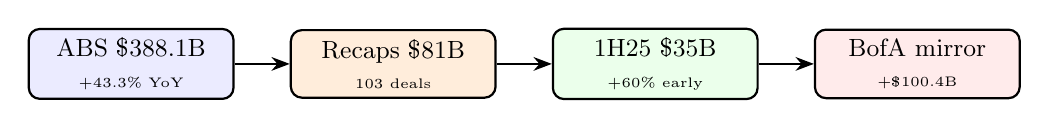
\begin{tikzpicture}[thick, node distance=0.6cm]
  \node[draw, rounded corners, fill=blue!8, minimum width=2.6cm, align=center, font=\small] (abs) {ABS \$388.1B \\ \tiny +43.3\% YoY};
  \node[draw, rounded corners, fill=orange!14, minimum width=2.6cm, align=center, font=\small, right=0.7cm of abs] (recap) {Recaps \$81B \\ \tiny 103 deals};
  \node[draw, rounded corners, fill=green!8, minimum width=2.6cm, align=center, font=\small, right=0.7cm of recap] (h125) {1H25 \$35B \\ \tiny +60\% early};
  \node[draw, rounded corners, fill=red!8, minimum width=2.6cm, align=center, font=\small, right=0.7cm of h125] (mirror) {BofA mirror \\ \tiny +\$100.4B};
  \draw[->, >={Stealth}] (abs) -- (recap);
  \draw[->, >={Stealth}] (recap) -- (h125);
  \draw[->, >={Stealth}] (h125) -- (mirror);
\end{tikzpicture}
\caption{Two Day-1 machines and one Day-N mirror. ABS issuance and dividend recap volume both running hot into 2025, then one bank's \$100.4B return to book when the QSPE permission slip died. Same loan from slow memory, taken many times, partly returned when one gate closed.}
\label{fig:timeline-machines}
\end{figure}

\section{Dividend recaps: the parallel track}

A dividend recapitalization, or dividend recap, is simpler. A company owned by a private fund borrows more and uses the new debt to pay its owners a dividend. The company is now more levered. The owners have cash. Fees are taken at the deal table. The slow vault, in the form of higher leverage and higher debt service, stays inside the company.

\textit{Measured, market tape via PitchBook and LCD as summarized in \texttt{divrecap\_market\_v1.json}:} \$81B in 2024, near record, across 103 deals, with institutional volume up about 500\% off 2023. That pace continued into 2025: \$35B in first half 2025, and \$22.4B by mid February 2025 alone, up 60\% year over year, with high yield bonds entering the recap funding mix at 7.36\% after a period when recaps were funded almost entirely by loans at 91\% share.

Those are not small numbers drifting sideways. They are a second Day-1 machine running alongside ABS, pulling future cash into present payouts. One machine securitizes tradable pools. The other leveres operating companies and dividends the proceeds. Both share the same time shape. Present fee takers are paid in full at close. Future holders, later lenders, later employees, later creditors, inherit the higher $S_t$.

Academic measurement now confirms this is structural, not anecdotal. \textit{Measured, first academic census NBER working paper w33435 as extracted in \texttt{divrecap\_nber\_extract\_v1.json} and \texttt{divrecap\_market\_v1.json}:} 61,628 US leveraged buyouts collapse to 1,572 dividend recaps, which is 2.6\% of deals but 9.3\% of volume. That concentration matters. A small share of deals moves a large share of dollars. Between 36\% and 43\% of general partners have done at least one recap. In the Gupta UNC 2024 companion, causal stakeholder estimates accompany the census. The channel is now census measured as a recurring type, not an outlier story.

The census also measures who gets recapped and what changes at the target. \textit{Measured, same NBER extract:} targets average 3.6 times total value to paid in against 2.7 times for overall buyouts. Gross profit change averages plus 105\% in recapped targets against minus 18\% in controls. Debt to EBITDA moves up 67 percentage points for recaps against down 34 points for controls. Distress frequency is 12.9\% for recapped firms against 9.8\% for controls. The pattern selects healthier firms, levers them, and leaves modestly elevated distress. Healthy in, more levered out, with the fee taken in between.

Two caveats travel with that census. The single deal fee waterfall that follows is widely cited but not census measured, and contested recaps where solvency is litigated are allegations, not holdings, until a court decides. We keep those grades separate.

\section{One deal, one waterfall, one contested edge}

\textit{Analogical on the fee waterfall shape; measured on the single deal citation and on the existence of contested filings.}

At single deal scale the shape is easy to see. The widely cited example in Vardi 2013, held in \texttt{divrecap\_nber\_extract\_v1.json}, records an \$85M payout that produced a 370\% return on equity for sponsors at that deal's close. That is Day-1 in one number. A payout taken now, a return crystallized now, a company left to service the new debt over the slow years. Whether that specific 370\% is typical does not matter for the mechanism. That it is cited as a real deal matters for existence. The channel can carry 370\% to sponsors while the company carries the leverage forward.

\textit{Analogical, schematic, not a filing reconstruction:} picture the fee waterfall in a leveraged recap. Transaction fees sit at the top, monitoring fees in the middle, financing fees alongside, equity dividend at close. Each is paid from proceeds or from the new debt before the company earns the cash to service it. The waterfall is analogical because the exact split varies by deal and by management services agreement, but the ordering is not analogical. Present fees prime future service. That ordering is arithmetic.

The contested edge is where the slow vault's bill arrives in court. \textit{Measured as filings that exist, not as decided truth:} creditors have alleged in cases including Buffets funded by Caxton Iseman, KB Toys involving Bain in 2012, and Cerberus with Steward, that dividend recaps rendered firms insolvent or left them unable to survive a downturn. Those are allegations of $Q_t$ suppressed while $S_t$ rose, with insolvency as the claimed wall. We grade them as contested extractions, measured as docket entries and press filings, not as holdings. The mechanism they allege is always the same. Economics upstreamed as dividend and fees, liabilities left downstream, recourse stopping at the corporate boundary.

One sentence should stay with you. When you see an \$85M Day-1 payout that books 370\% to sponsors inside a \$81B year of recaps, you are not looking at an outlier. You are looking at the same time transfer the ABS machine does, done instead inside operating companies and paid as dividend rather than as bond proceeds.

\section{Why damping sleeps and why walls are discrete}

A ledger does not enforce itself. People do, or they do not. Write off discipline sounds technical. In practice it is a calendar and a courage problem. When does someone have to look, and will they write what they see.

In funds the calendar is the monthly net asset value. In banks it is the provisioning cycle and the quarterly call report. In operating companies it is the impairment test and the audit committee that signs it. Each is a night shift that is supposed to compare the fast story against the slow stock and force $Q_t$ to catch up. When the night shift is well lit, well paid to be honest, and separate from the desk that books $E_t$, $Q_t$ catches up and $S_t$ cannot compound far. When the night shift is dim, rushed, or paid by the same desk that booked $E_t$, $Q_t$ sleeps and $S_t$ grows.

Three small frictions are enough to put damping to sleep. First, the cost of looking is paid now and the benefit arrives later, and later has no representative in the room. Second, the person who booked $E_t$ is often the person who must approve $Q_t$, so admitting $Q_t$ is admitting their own prior mark was wrong. Third, everyone is doing it at the same time, so the peer group that should supply discipline instead supplies cover. None of these needs collusion. Each is just a quiet incentive to look away for one more period.

Walls are discrete for a related reason. Maturities do not drift. They expire on a date. Facilities do not fade. They either roll or they do not. A conduit either finds buyers for its new paper or it does not. A dividend recapped company either covers its new interest from cash flow or it needs a new facility to cover it. The distribution of outcomes is therefore not a gentle slope. It is a cliff with a long approach. You can walk the approach for years while inspections say performing. Then one date does not clear and recognition jumps. That jump is why $S_t$ is a vault and not a curve. You fill it grain by grain, then the door is forced at once.

Put those two facts together and the timing of loss is not mysterious. Slow $S_t$ rises while damping sleeps, fast entries keep printing Day-1 fees, and a discrete wall converts the stock to a flow in one period. Anyone who tells you later that the wall was a surprise is selling you a story about volatility. The vault was not volatile. It was filling.

\section{How to read a census without being fooled}

A census is only useful if you know how to read it. The NBER census that counts 61,628 buyouts down to 1,572 recaps is not a claim that every recap is the same. It is a map of where the parallel track runs hottest and what changes when it does.

Read concentration first. If 2.6\% of deals carry 9.3\% of volume, the average recap is larger and more levered than the average buyout. That matters for $S_t$ because larger deals create larger stocks per deal while using the same small number of gates to do it. One large recap can move more future debt service than five small buyouts combined, and it can do it with one set of transaction fees taken at close.

Read selection second. The census finds that recapped targets average 3.6 times total value to paid in against 2.7 times for the average buyout, with gross profit up 105\% against down 18\% for controls. That is not a story about weak firms being milked. It is a story about strong firms being levered precisely because they can bear more debt for a while. Health selects for capacity to carry $S_t$ forward. That selection is why distress rises only modestly in the averages, from 9.8\% to 12.9\%, even while Debt to EBITDA moves up 67 percentage points against down 34 for controls. The healthy can carry more before they break, so the stock can be larger before the wall.

Read the fee waterfall third, and read it with its grade. \textit{Analogical, schematic.} Transaction fees, monitoring fees under management services agreements that require no work to be performed and are rebated only 70 to 72\% on average, financing fees, and the dividend itself, each is paid before the company must earn the cash to service the new debt. The SEC has fined several general partners and extracted \$4.5M plus \$5.4M repaid in one offset failure action alone, with fee offsets a perennial exam priority. That enforcement is measured. The waterfall shape inside any given deal remains analogical because the split varies, but the ordering is not analogical. Present fees prime future service, every time.

\begin{table}[h]
\centering
\small
\caption{What the first academic census finds when a firm is dividend recapped, NBER w33435 as extracted}
\label{tab:recap-census}
\begin{tabular}{p{4.2cm} p{2.6cm} p{2.6cm}}
\toprule
Measure & Recap target & Control buyout \\
\midrule
Share of sample & 1,572 / 61,628 (2.6\%) & remainder \\
Share of volume & 9.3\% & 90.7\% \\
GPs ever having done one & 36 to 43\% of GPs &  \\
TVM (total value to paid in) & 3.6 times & 2.7 times \\
Gross profit change & +105\% & --18\% \\
Debt to EBITDA move & +67 pp & --34 pp \\
Distress frequency & 12.9\% & 9.8\% \\
\bottomrule
\end{tabular}
\end{table}

Read distress last, and read it slowly. A rise from 9.8\% to 12.9\% looks small until you multiply it by a larger deal, a larger debt load, and a larger $S_t$ per deal. Three extra distressed firms out of a hundred does not sound like a wall. Multiply by \$81B of 2024 issuance and by the refinancing wall that clusters two to three years forward, and the same three points become a filing wave that arrives on one calendar, not spread over ten.

The census also helps you see what the contested cases allege. In Buffets, in KB Toys in 2012, in Cerberus with Steward, the claim is not that recaps always fail. It is that at that deal, on that date, $Q_t$ was suppressed while $S_t$ was raised enough that insolvency followed. Those are allegations measured as dockets, not holdings, and we keep them graded that way. The mechanism they allege is always the time shape you already know. Day-1 dividend and fees now, levered company carrying the stock, wall later.

One habit makes you harder to fool. Whenever you see a Day-1 number, ask where the slow vault received its offset. If you can name the vault, name its $Q_t$ calendar, and watch whether $Q_t$ is rising with $E_t$, you have a checkable view. If you cannot, you have a story.

\section{The mirror event: when slow memory snaps back}

If timeline games could run forever, there would be no fact. They cannot. Slow memory eventually forces its way back onto the fast ledger. That forcing has a date and a dollar amount, and it was public.

For a new reader, a \textbf{SPV}, or Special Purpose Vehicle, is the legal shell that holds securitized assets off the sponsor's balance sheet. A \textbf{QSPE}, or Qualifying Special Purpose Entity, was the accounting category that let certain SPVs stay off balance sheet without ongoing consolidation tests. An \textbf{SPV} is the box. A \textbf{QSPE} was the permission slip that said the box did not count.

On January 1, 2010, the permission slip died. SFAS 166 and 167, the consolidation guidance, killed the QSPE concept. Boxes that had counted as off book the day before now had to be tested for consolidation. If the sponsor controlled them or bore their risks, they came back on book.

\textit{Measured, Bank of America 2010 10-K, accession 0000950123-11-018743, artifact panel \texttt{edgar\_VIE\_panel\_prose\_v1.json} and \texttt{edgar\_K\_panel\_v1.json}:} Bank of America consolidated \$100.4B of assets on January 1, 2010, consisting of \$69.7B of credit card trusts plus \$30.7B of special purpose entities including multi seller conduits, with \$106.7B of liabilities including \$84.4B of long term debt, and a \$6.2B net of tax charge to retained earnings.

Read that again. One hundred point four billion dollars reappeared on one bank's balance sheet in one quarter because a rule changed. Not because the economics changed that quarter. The economics had been there. The permission to keep them off book changed. The slow vault opened on camera.

For a new reader who has never seen a bank footnote, that is the whole lesson in one event. What Day-1 pulls out, Day-N forces back. The hundred billion did not become real on January 1, 2010. It became visible. The transfer from later holders to earlier fee takers, the $S_t$ that had compounded off book through years of issuance and recap, could no longer roll past the reporting window once the window moved. Recognition $\psi$ jumped toward one in a single period because walls are discrete, exactly as the $S_t$ law predicts.

The mirror proves three things at once. First, the stock was real all along, not a theory. Second, damping is not optional. When $Q_t$ is suppressed by design, $S_t$ does not vanish, it waits. Third, a rule change can be a wall. Maturity walls and funding walls are not the only discrete events that force recognition. An accounting wall does the same work. The cohort that thought it had bought a clean balance sheet inherited the stock that prior cohorts had been paid to create.

Keep the BofA number next to the ABS and recap numbers and the picture sharpens. ABS issuance at \$388.1B plus 43.3\% growth, dividend recaps at \$81B and still growing into 2025, and one bank's Day-N return of \$100.4B after years of Day-1 extraction, these are not three separate stories. They are the same loan from slow memory, taken many times, by many hands, and then partly returned when one gate closed. The residual, the part not returned, is $S_t$ still sitting in vaults whose gates have not yet closed.

Two details deserve care. The BofA charge to retained earnings was net of tax, \$6.2B, which tells you the consolidation was not cosmetic. It hit equity. And the multi seller conduit piece inside the \$30.7B is instructive. Conduits are the purest timeline vehicle. They fund long assets with short paper and roll forever, or until they cannot. Bringing them back on book is the literal return of a timeline bet to the balance sheet that made the bet.

\begin{figure}[h]
\centering
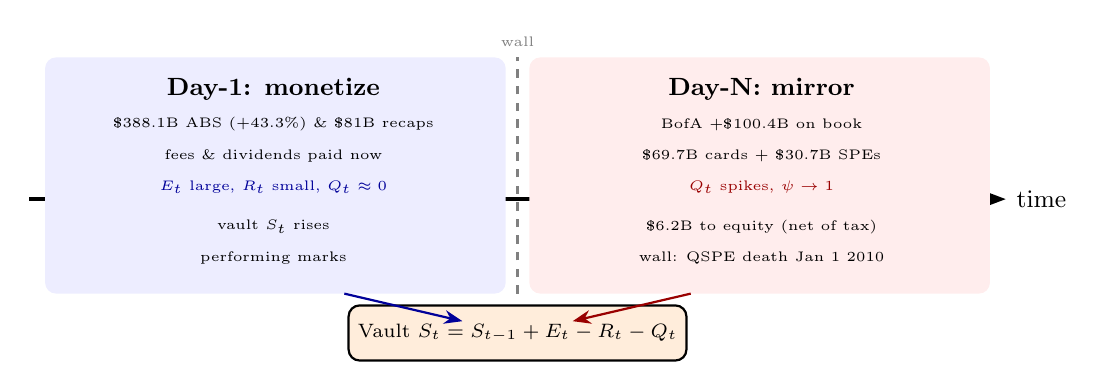
\begin{tikzpicture}[thick, >=Stealth]
  % timeline axis
  \draw[->, very thick] (-6.2,0) -- (6.2,0) node[right, font=\small] {time};
  % Day-1 region
  \fill[blue!7, rounded corners] (-6, -1.2) rectangle (-0.15, 1.8);
  \node[align=center, font=\small\bfseries] at (-3.1, 1.4) {Day-1: monetize};
  \node[align=center, font=\tiny] at (-3.1, 0.95) {\$388.1B ABS (+43.3\%) \& \$81B recaps};
  \node[align=center, font=\tiny] at (-3.1, 0.55) {fees \& dividends paid now};
  \node[align=center, font=\tiny, text=blue!60!black] at (-3.1, 0.15) {$E_t$ large, $R_t$ small, $Q_t \approx 0$};
  \node[align=center, font=\tiny] at (-3.1, -0.35) {vault $S_t$ rises};
  \node[align=center, font=\tiny] at (-3.1, -0.75) {performing marks};
  % Day-N region
  \fill[red!7, rounded corners] (0.15, -1.2) rectangle (6, 1.8);
  \node[align=center, font=\small\bfseries] at (3.1, 1.4) {Day-N: mirror};
  \node[align=center, font=\tiny] at (3.1, 0.95) {BofA +\$100.4B on book};
  \node[align=center, font=\tiny] at (3.1, 0.55) {\$69.7B cards + \$30.7B SPEs};
  \node[align=center, font=\tiny, text=red!60!black] at (3.1, 0.15) {$Q_t$ spikes, $\psi \to 1$};
  \node[align=center, font=\tiny] at (3.1, -0.35) {\$6.2B to equity (net of tax)};
  \node[align=center, font=\tiny] at (3.1, -0.75) {wall: QSPE death Jan 1 2010};
  % vault in middle
  \node[draw, rounded corners, fill=orange!14, minimum width=2.0cm, minimum height=0.7cm, align=center, font=\scriptsize] at (0, -1.7) {Vault $S_t = S_{t-1}+E_t-R_t-Q_t$};
  \draw[->, blue!60!black, thick] (-2.2, -1.2) -- (-0.7, -1.55);
  \draw[->, red!60!black, thick] (2.2, -1.2) -- (0.7, -1.55);
  % wall line
  \draw[very thick, dashed, gray] (0, -1.2) -- (0, 1.8) node[above, font=\tiny, gray] {wall};
\end{tikzpicture}
\caption{Day-1 vs Day-N mirror timeline. Left: Day-1 monetization (ABS \$388.1B at +43.3\% YoY, recaps \$81B) pays fees now while $S_t$ rises off book ($Q_t \approx 0$). Right: Day-N mirror (BofA Jan 1 2010: +\$100.4B assets, +\$106.7B liabilities, \$6.2B equity charge) forces $S_t$ back on book when QSPE dies. Dashed wall is discrete: $\psi$ jumps $0 \to 1$ in one period. Sources: \texttt{sifma\_abs\_2024\_v1.json}, \texttt{divrecap\_market\_v1.json}, BofA 10-K acc. 0000950123-11-018743, \texttt{edgar\_K\_panel\_v1.json}.}
\label{fig:timeline-mirror}
\end{figure}

This chapter's grade is steady. SIFMA tape and census counts are measured. The BofA mirror is measured in a primary filing. The single deal 370\% and the contested insolvency allegations are measured as cited instance and as contested filings respectively. Schematic waterfalls remain analogical on purpose, labeled as such, because the deal level split varies. The $S_t$ law itself stays formal, an identity that becomes empirical only when mapped to provisions and write offs line by line, which happens in later chapters.

The wall is never a surprise to the vault. It is only a surprise to those who were paid not to look at it.

Timeline tells you when loss will arrive. Entity tells you where it will be parked so that, when it arrives, the claim against it is already small. Turn the page and we redraw the boundary.


\chapter{Entity: Redrawing the Boundary}
\label{ch:entity}

\textit{Grade for this chapter: measured on pod thresholds, unwinds, VIE panel, consolidation, and court holdings; analogical where we describe fee paths inside a pod or a trust before a filing line proves them.}

If timeline tells you when loss arrives, entity tells you where it will be sitting when it arrives so that the claim against it is already small. The move is simple. Redraw the boundary so the promise attaches to a shell while the economics were already upstreamed to the sponsor. On paper failure is contained. In substance the sponsor was paid first.

For a child, a boundary is a fence you can see. For a firm, a boundary is a legal test someone can litigate. That difference is the whole game. Fences hold unless you move them. Legal boundaries are drawn to order. Move the fence, move the reachable assets, and you move the recovery without changing the accounting total by much. This chapter makes that move checkable.

Two comforts compete here and both are decoys. The diversification story says many boxes mean many independent bets. But boxes share funding desks, primes, and crowded factors, so fifty labels can be one trade with fifty names. The paperwork story says the structure is too complex to judge. But the test never changes and fits one sentence: name the reachable assets, state the recourse terms, compute the cap. What remains standing: containment on paper, upstreamed economics in substance.

\section{The boundary organ}

Every living system needs a boundary organ. Skin decides what counts as inside the body. A bank charter decides what counts as inside the bank. A fund decides what counts as inside a pod, even when the pod lives on the same balance sheet as three hundred other pods. Without a boundary, attribution fails and loss floats. With a boundary, loss can be assigned, and also gerrymandered.

For a new reader, think of the boundary organ as the fence that constitutes the relation it divides. It does not merely mark inside versus outside. It decides what crosses and what does not. In markets the fence is legal recourse. If a vehicle fails and the sponsor has no contractual obligation to fund it, then the creditor's reachable assets $A$ are the vehicle's assets only. If vehicle $A$ is small, the collectability cap $K(A)$ is small regardless of how good the creditor's legal arguments are. Saying you have a claim on the group is not the same as having a claim you can enforce. $K$ makes that difference explicit as $\phi = \min\{\psi H, K\}/H$, the paid share after gating and capping.

That is why entity engineering is powerful. It works before any gate is litigated. It chooses whose $K$ binds and whose $K$ does not, before anyone files.

We keep one discipline throughout this chapter. We name the envelope, we state the recourse terms, and we state the reachable $A$. Without those, $\phi$ is just a number. With them, it is a mechanism you can audit.

\section{The pod shop: a laboratory of the boundary}

The cleanest laboratory of the boundary organ in modern finance is the pod shop. For a new reader, a \textbf{pod} is a team that owns a bounded book and a bounded loss. The pod receives allocated capital, risk limits, and a strategy sleeve that is supposed to be hedged on measured factors. The platform provides capital allocation, risk monitoring, trading operations, and a funding desk, but does not by default cross margin risk across pods. Each pod is meant to be a watertight compartment. Water may fill one without sinking the ship, if the walls hold.

Three intended effects follow. The blast radius is bounded when a pod is wrong. Attribution is clean so winners and losers are known and can be cut or fed. Damping is forced at the pod wall before loss becomes system loss. That is the theory. Whether the walls hold depends on what is shared across them: a common funding desk, a common prime broker, a common reinsurance or guarantee, or one crowded factor that makes many pods wrong at once. Labels diversify. Factors do not.

\textit{Measured, industry documented in \texttt{pods\_goodhart\_v1.json} and corroborated in trade press:} Millennium halves capital at minus 5\% and terminates a pod at minus 7.5\%, automatically, with 15 to 20\% annual portfolio manager turnover treated as a feature rather than a failure. Pods run \$100 to \$200M each across 320 plus teams at about \$79B of assets under management as of September 2025. Citadel's equivalents are individually negotiated rather than formulaic, with \$25B returned to investors since 2017 as part of capacity management. Those thresholds are now industry fact, not lore.

For a new reader, halving at minus 5\% means the platform pulls half the pod's capital when it is down five percent, and termination at minus 7.5\% means the book is liquidated and the team is cut when down seven and a half. The rule has memory. It does not reset because the manager wants a second chance. It resets only when risk does, after a cool down. That is damping with hysteresis, a brake that stays on.

Why fifteen to twenty percent turnover is a feature becomes clear once you see the alternative. Without a binding breaker, a losing pod can lobby, hedge cosmetically, and survive to gamble for resurrection. With a binding breaker, the platform treats pods as experiments. Many are run, some are killed, capital moves to survivors. The ledger of who failed is literal. That is also why the pod shop is checkable in a way older conglomerates were not. You can count pods, count cuts, and watch whether the platform honors its own thresholds when crowded.

\begin{figure}[h]
\centering
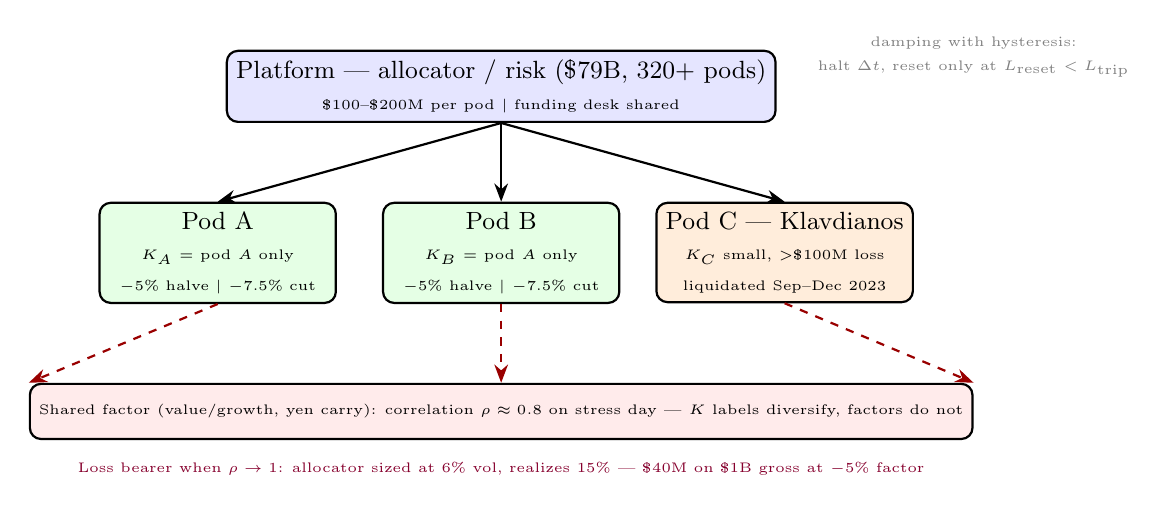
\begin{tikzpicture}[thick, >=Stealth, font=\small]
  % Platform apex
  \node[draw, rounded corners, fill=blue!10, minimum width=5.2cm, minimum height=0.9cm, align=center] (plat) {Platform — allocator / risk (\$79B, 320+ pods)\\ \tiny \$100--\$200M per pod \textbar\ funding desk shared};
  % Pods
  \node[draw, rounded corners, fill=green!10, minimum width=3.0cm, minimum height=1.0cm, align=center, below=1.0cm of plat, xshift=-3.6cm] (pod1) {Pod A \\ \tiny $K_A$ = pod $A$ only \\ \tiny $-$5\% halve \textbar\ $-$7.5\% cut};
  \node[draw, rounded corners, fill=green!10, minimum width=3.0cm, minimum height=1.0cm, align=center, below=1.0cm of plat] (pod2) {Pod B \\ \tiny $K_B$ = pod $A$ only \\ \tiny $-$5\% halve \textbar\ $-$7.5\% cut};
  \node[draw, rounded corners, fill=orange!14, minimum width=3.0cm, minimum height=1.0cm, align=center, below=1.0cm of plat, xshift=3.6cm] (pod3) {Pod C — Klavdianos \\ \tiny $K_C$ small, $>$\$100M loss \\ \tiny liquidated Sep--Dec 2023};
  % Arrows from platform
  \draw[->] (plat.south) -- (pod1.north);
  \draw[->] (plat.south) -- (pod2.north);
  \draw[->] (plat.south) -- (pod3.north);
  % Shared factor arrow
  \node[draw, rounded corners, fill=red!8, minimum width=10.5cm, minimum height=0.7cm, align=center, font=\tiny, below=1.0cm of pod2] (factor) {Shared factor (value/growth, yen carry): correlation $\rho \approx 0.8$ on stress day — $K$ labels diversify, factors do not};
  \draw[->, red!60!black, dashed, thick] (pod1.south) -- (factor.north west);
  \draw[->, red!60!black, dashed, thick] (pod2.south) -- (factor.north);
  \draw[->, red!60!black, dashed, thick] (pod3.south) -- (factor.north east);
  % Breaker annotation
  \node[align=left, font=\tiny, text=gray] at (6.0, 0.55) {damping with hysteresis:};
  \node[align=left, font=\tiny, text=gray] at (6.0, 0.22) {halt $\Delta t$, reset only at $L_{\text{reset}} < L_{\text{trip}}$};
  % Loss bearer note
  \node[align=center, font=\tiny, text=purple!70!black, below=0.15cm of factor] {Loss bearer when $\rho \to 1$: allocator sized at 6\% vol, realizes 15\% — \$40M on \$1B gross at $-5$\% factor};
\end{tikzpicture}
\caption{Pod hierarchy with $K$ labels. Platform allocates \$100--\$200M per pod (\$79B, 320+ teams, \texttt{pods\_goodhart\_v1.json}) with $K$ at pod $A$ only under no cross-margin. Breakers ($-$5\% halve, $-$7.5\% terminate, Millennium automatic; Citadel negotiated; 15--20\% turnover as feature) bound idiosyncratic loss. Dashed red is the shared factor that bypasses $K$ labels: 50 pods at \$20M gross with $\beta \approx 1$ lose \$40M together at $-5$\% factor when $\rho \to 0.8$ despite $K_A, K_B, K_C$ walls holding individually. Instances: Klavdianos \$100M (Bloomberg Dec 12--13 2023, liquidation Sep--Dec, \texttt{pods\_single\_pod\_autopsies\_v1.json}), Aug 2024 six-pod cluster (Fitzgibbon/Ying/Corones/Murayama/Motegi/Cox) after Nikkei $-12.4$\% and USD/JPY $161 \to 142$.}
\label{fig:pod-hierarchy}
\end{figure}

\noindent\textit{Breaker arithmetic, worked:} a \$150M pod at $-5$\% has lost \$7.5M and is halved to \$75M of capital; at $-7.5$\% the loss is \$11.25M and the book is cut. That is not a suggestion. At Millennium it is automatic. The August 2024 cluster (at least six pods cut across Millennium, Balyasny, BlueCrest after the yen carry snapped — VIX intraday $>65$, Nikkei $-12.4$\% on Aug 5) is that arithmetic executed at scale: Hedgeweek explicates capital partially withdrawn after 5\% and dismissed after about 7\%, Bloomberg's Aug 30 tally names Fitzgibbon in Houston, Ying and Corones in Asia, Murayama and Motegi in JGB, Cox in Hong Kong, each under the same rule. The unwind is the breaker working, not failing. What fails is the allocator's belief that many $K$ labels meant many bets.

\section{When walls are stress tested in public}

Thresholds on paper are one thing. Walls under stress are another. This is where grading matters. Platform level unwinds are measured. Single pod autopsies are now also measured in trade press. Internal backstop plumbing remains analogical until a prime letter or filing proves it.

\textit{Measured, platform level, \texttt{pods\_chaebol\_instances\_v1.json}:} three public stress tests. First, Balyasny 2018, the firm's first annual loss at minus 7\%, with a 20\% staff cut, published postmortems, and a rebuild from \$6B to \$27B on diversification after the drawdown. Walls held in the sense that the platform survived and re diversified, but the year was the first time the breaker logic was seen to bite at firm scale.

Second, Eisler Capital's 2025 closure, attributed in press to talent war costs and scale economics that made the platform's cost base unsustainable even before market stress arrived. That is a boundary failure by economics, not by correlation. The organ that was stressed was not the pod wall but the platform's ability to fund the lab itself.

Third, first quarter 2026, synchronized drawdowns of minus 4.3\% and minus 4.5\% at Balyasny and ExodusPoint on correlation breakdown. That is the finding the whole pod theory turns on. Minus four percent at two independent platforms at the same time, from the same factor dislocation, despite pod walls inside each platform. Walls hold idiosyncratic risk, not crowding. When the crowded factor moves, many pods are the same trade with different logos and the platform is one bet with many names.

\textit{Measured, single pod level, now sourced in \texttt{pods\_single\_pod\_autopsies\_v1.json} with Bloomberg headlines held via Bloomberg Law mirrors and trade-press syndication:} two autopsies fill the gap that was open for two years. One is Balyasny event driven credit pod head George Klavdianos in London, reported by Bloomberg on December 12 and 13, 2023 (Lucca de Paoli, Nishant Kumar, Irene Garcia Perez; mirror at \texttt{news.bloomberglaw.com/capital-markets} confirming headline and deck) as a loss of more than \$100M including unwind costs, with liquidation beginning in September 2023 and team exit in December, representing about one percent of gross assets in a credit sleeve that contextual reporting (eFinancialCareers) puts near five percent of firm assets. eFinancialCareers Dec 13 notes the FCA register still showed Klavdianos at BAM at time of writing and attributes the \$100M to the US credit sleeve plus Klavdianos sleeve; eFinancialCareers 2024 confirms rehire at Millennium London after 3.5y at BAM and 6.5y at Citadel. The other is the August 2024 yen carry unwind, where at least six pods were reported shut across Millennium, Balyasny, and BlueCrest after the yen carry snapped and global risk repriced (Bloomberg Aug 30: Nishant Kumar, Bei Hu, Takashi Nakamichi; Hedgeweek Sep 2 syndication listing all six names; MoneyControl Aug 26 on Ying/Corones Asia closures), with named managers including Ryan Fitzgibbon in Houston (industrials/energy), Shao Ying and Zachary Corones in Asia (index-rebalancing), Chiga Murayama and Yosuke Motegi in JGB trading, and Mark Cox in Hong Kong, under the same 5\% halve and 7.5\% terminate logic that Hedgeweek explicates as partially withdrawn after five percent and dismissed after about seven. Bloomberg's trigger tape is precise: Nikkei $-12.4$\% on Aug 5 (worst since 1987), TOPIX $-12$\%, VIX intraday $>65$, USD/JPY $161 \to 142$. Funds rebounded by Aug 23 ($+$1\% Schonfeld, $+$0.9\% LMR, $+$0.7\% Millennium month-to-date per Hedgeweek) — the platform survived because pods were cut. Adjunct same-quarter cut (Bloomberg Jun 27: Balyasny merger-arb team Adam Schwartz and Schonfeld's Eric Fritz) shows turnover as feature, not anomaly.

A note on what stays analogical after those autopsies. That breaker thresholds bind is now measured. That specific pods were cut under them is now measured. What internal backstop would have done if many pods tripped together, cross guarantees, shared funding, rehypothecation, or a platform level guarantee, remains unsourced until a filing says so. We assert the channel. Instances carry their own citations. Short sentences. Evidence graded.

For a new reader, the lesson is not that pods fail. It is that pods do exactly what they promise and no more. They bound idiosyncratic loss. They do not bound a factor that every pod loads through different names. If fifty pods are each long cheap value versus expensive growth through different securities, the host shows \$1B of diversified gross with \$20M per pod. A one day factor unwind of minus five percent with cross pod correlation at 0.8 turns that into one \$40M loss from a bet the allocator thought it did not have. Loss bearer: the allocator who sized at six percent volatility assuming zero cross pod beta, now facing fifteen percent realized.

\section{A four bank panel: where $K$ actually sits}

From pods we step to banks, because banks file. For a new reader, a \textbf{VIE}, or Variable Interest Entity, is the accounting name for an entity whose control is not decided by voting shares but by who bears its risks and rewards and who has power over its key decisions. If you sponsor a VIE, benefit from it, and control it, you consolidate it. If you do not, it can sit off balance sheet with a disclosed maximum exposure. A VIE is the modern name for the shell we have been calling an envelope.

\textit{Measured, EDGAR XBRL company facts plus Note prose across twelve filings, artifacts \texttt{edgar\_K\_panel\_v1.json} and \texttt{edgar\_VIE\_panel\_prose\_v1.json}:} maximum VIE exposure runs Citi \$54.8B on December 31, 2010, then JPMorgan \$28.6B on March 31, 2011, then Bank of America \$8.1B on June 30, 2010, then Wells Fargo \$0 on September 30, 2010. Distribution matches crisis severity exactly, from most off balance reachability to least, which is itself a check on the measure.

Put the shells next to them, also from XBRL and prose. Junior trust shells that fund capital, also called trust preferred vehicles, show Citi \$10.1B in 2012, JPMorgan \$2.3B in 2016, Bank of America absent in the XBRL tag for that vintage because the trusts were redeemed or renamed after the crisis, and Wells Fargo \$0.7B in 2020. Anchor them to on book long term debt so the scale is honest: Citi \$315.8B in 2025, JPMorgan \$267.9B in 2013, Bank of America \$317.8B in 2025, Wells Fargo \$174.7B in 2025. Those anchors tell you the VIE and trust numbers are not rounding error, but they are also not the whole balance sheet. They are the boundary layer where $K$ is chosen.

\begin{table}[h]
\centering
\small
\caption{Four bank $K$ placement panel, dollars, from XBRL company facts and 10-K and 10-Q prose}
\label{tab:entity-kpanel}
\begin{tabular}{p{2.0cm} p{2.9cm} p{2.9cm} p{2.9cm}}
\toprule
Bank & VIE max exposure & Junior trust shell & Long term debt \\
\midrule
Citi & \$54.8B (2010-12-31) & \$10.1B (2012) & \$315.8B (2025) \\
JPM & \$28.6B (2011-03-31) & \$2.3B (2016) & \$267.9B (2013) \\
BofA & \$8.1B (2010-06-30) & absent (redeemed or renamed) & \$317.8B (2025) \\
Wells & \$0 (2010-09-30) & \$0.7B (2020) & \$174.7B (2025) \\
\bottomrule
\end{tabular}
\end{table}

For a new reader, maximum exposure is the accounting phrase for reachable $K$ outside the reported boundary until drawn. It is the number the bank says it could lose if the off balance vehicle drew every facility. The economics are inside the prose that accompanies it. JPMorgan's 2010 Note 16, filed as accession 0000950123-11-019773 and held as \texttt{edgar\_VIE\_prose\_v1.json}, defines a sponsored VIE by four prongs and shows the plumbing. A sponsored VIE is one where the firm is principal beneficiary, or the vehicle securitizes firm assets, or it issues with the JPMorgan name, or it is a firm administered asset backed commercial paper conduit. Inside those conduits, maximum exposure on nonconsolidated firm administered multi seller conduits was \$24.8B at December 31, 2009, with deal specific liquidity of \$24.2B and program wide liquidity of \$13.0B plus \$2.0B of enhancements. The XBRL tag for Variable Interest Maximum Exposure to Loss at December 31, 2010 prints \$27.8B. Prose and machine readable tag agree within conduit growth. The enhancement cap written into the conduit documents is a $K$ cap in contract language, not a metaphor.

Citi in the same vintage tells the opposite disclosure technology. Mortgage securitizations are VIEs and maximum exposure equals carrying amount, with Omni Trust commercial paper funding facility of \$2.5B at December 31, 2009 under the Federal Reserve's Commercial Paper Funding Facility, as filed in accession 0001206774-11-000316. Wells Fargo in 2010 discloses no VIE or securitization vehicles at all, an on balance whole loan model, consistent with XBRL VIE of \$0 filed in accession 0000950123-11-018541. The panel is not just a table then. It is a technology choice. JPMorgan runs conduits with capped enhancements. Citi runs securitizations where max equals carrying. Wells runs without either. BofA is about to show what happens when the technology is forced to change.

\section{The mirror event again, now as entity repair}

The same BofA number that closed the timeline chapter belongs here as an entity event. SFAS 166 and 167 killed the \textbf{QSPE} permission slip on January 1, 2010. The rule did not create economics. It moved boxes back inside the boundary that owned them.

\textit{Measured, Bank of America 2010 10-K, accession 0000950123-11-018743, same panel:} consolidation on January 1, 2010 of \$100.4B of assets, split as \$69.7B of credit card trusts plus \$30.7B of special purpose entities including multi seller conduits, with \$106.7B of liabilities including \$84.4B of long term debt, and a \$6.2B net of tax charge to retained earnings.

In $K$ terms, reachable $A$ for card and conduit creditors moved back on balance sheet. $K$ visibly rose inside the bank and fell outside it. Where before a trust creditor had recourse to a small vehicle $A$, now the same creditor had recourse to Bank of America $A$. That is the boundary organ repaired by rule, not by choice, and the \$6.2B charge tells you it was not cosmetic.

The evolution to 2020 matters because it answers whether banks rebuilt the old off balance share once the crisis passed. \textit{Measured, eight filings 2015 and 2020, artifact \texttt{edgar\_VIE\_evolution\_2015\_2020\_v1.json}:} JPMorgan consolidated VIE beneficial interests fall from \$41.9B in 2015 to \$17.6B in 2020, muni vehicle maximum exposure from \$6.3B in 2014 to \$3.8B in 2015. Bank of America keeps the 2010 consolidation on book under the primary beneficiary test with unconsolidated VIEs disclosed in Note 6. Citigroup holds its disclosure technology constant, maximum exposure equals carrying amount in Note 22. Wells Fargo, VIE free in 2010, carries securitization and VIE notes by 2015 to 2020 on its mortgage book after Wachovia. No bank rebuilds pre crisis off balance reachability by 2020. Regulation moved $K$ on book after 2010 and kept it there, which is also why the next frontier of boundary engineering is not conduits but the corporate forms this chapter turns to next.

\begin{figure}[h]
\centering
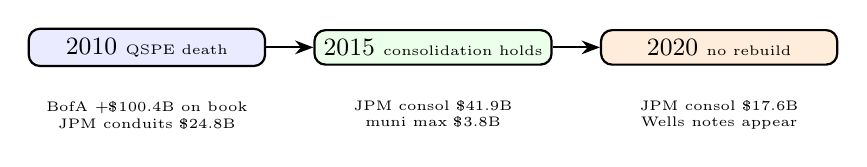
\begin{tikzpicture}[thick, node distance=0.6cm]
  \node[draw, rounded corners, fill=blue!8, minimum width=3.0cm, align=center, font=\small] (t10) {2010 \tiny QSPE death};
  \node[draw, rounded corners, fill=green!8, minimum width=3.0cm, align=center, font=\small, right=of t10] (t15) {2015 \tiny consolidation holds};
  \node[draw, rounded corners, fill=orange!14, minimum width=3.0cm, align=center, font=\small, right=of t15] (t20) {2020 \tiny no rebuild};
  \draw[->, >={Stealth}] (t10) -- (t15);
  \draw[->, >={Stealth}] (t15) -- (t20);
  \node[below=0.3cm of t10, font=\tiny, align=center] {BofA +\$100.4B on book \\ JPM conduits \$24.8B};
  \node[below=0.3cm of t15, font=\tiny, align=center] {JPM consol \$41.9B \\ muni max \$3.8B};
  \node[below=0.3cm of t20, font=\tiny, align=center] {JPM consol \$17.6B \\ Wells notes appear};
\end{tikzpicture}
\caption{$K$ evolution 2010 to 2020 after the QSPE was killed. Conduit footprints shrink or persist, never rebuild. The boundary repair sticks.}
\label{fig:entity-ktimeline}
\end{figure}

\section{The Texas Two Step: a boundary machine tested three times}

For a new reader, a \textbf{divisional merger} under Texas Business Organizations Code section 1.002(55)(A) is a statute that lets a company split into two or more companies in one filing, allocating assets to one survivor and liabilities to another. It is lawful per se. The question in each case is what it is used for and whether bankruptcy is the right forum for what follows.

The machine nicknamed the Texas Two Step works like this. An operating company with large tort liabilities uses a divisional merger to split into two. One successor, call it NewCo, receives most operating assets. The other, call it LiabilityCo, receives the tort liabilities and a funding agreement that says NewCo, and sometimes a parent, will fund LiabilityCo's costs and obligations. LiabilityCo then files for Chapter 11 and proposes a channeling injunction or trust that would resolve the tort claims inside bankruptcy, with NewCo continuing to operate outside it. Formal recourse for tort claimants is now capped at LiabilityCo $A$ plus whatever the funding agreement promises, not at NewCo or group $A$. If LiabilityCo $A$ is small, $K$ for tort creditors is small regardless of $\psi$ on the underlying harm.

We grade this carefully because courts have now spoken three times. Holdings are measured. Motives remain litigated.

\textit{Measured, holdings in \texttt{tt\_holdings\_v1.json} with full opinion texts in \texttt{tt\_opinion\_texts2.json}, 78,000 plus 87,000 characters held:}

First, \textit{In re LTL Management LLC}, 64 F.4th 84, Third Circuit 2023. Mechanism: October 12, 2021 divisional merger under Texas Business Organizations Code section 1.002(55)(A) split Old Consumer into LTL, which received talc liabilities, plus New Consumer, which received operating assets, plus a Funding Agreement giving LTL funding rights against New Consumer and Johnson and Johnson. Holding: dismissed under section 1112(b). Only a putative debtor in financial distress may access Chapter 11 for a valid bankruptcy purpose. LTL was not in financial distress, so the filing was dismissed.

Second, \textit{Bestwall LLC}, Fourth Circuit No. 22-1135, June 20, 2023. Mechanism: 2017 divisional merger under the same Texas statute splitting Old GP into Bestwall plus New GP, plus a funding agreement obligating New GP to cover Bestwall's expenses and obligations while its operating assets sit out of tort reach. Holding: distinguishes LTL on the ground that no good faith or financial distress challenge was raised in this proceeding. The court describes the merger mechanics verbatim and leaves the door open where LTL closed it, but the machine's legality per se is not endorsed as a broad channeling tool.

Third, \textit{In re Red River Talc LLC}, Southern District of Texas No. 24-90505, filed September 20, 2024. This is the repeat attempt by the same sponsor after LTL. Mechanism: prepackaged plan proposing a \$9B trust with 90,000 claimants voting. Outcome: confirmation denied and case dismissed March 31, 2025 by Judge Lopez. Johnson and Johnson announced no appeal, returned to the tort system, and reversed about \$7B in reserves. Artifact \texttt{redriver\_koreazinc\_v1.json} holds the trade press and docket synthesis.

Three filings, three dismissals, two jurisdictions. The sponsor that invented the repeat attempt announced its end. For this book the point is not schadenfreude. It is $K$. Where before tort claimants would have had recourse to operating $A$, after the split they faced a small LiabilityCo $A$ plus a funding agreement whose promise is only as good as its terms and the willingness of a court to let bankruptcy rewrite tort recourse. The boundary was moved by statute, the cap was moved by contract, and courts declined to bless the resulting $K$.

A note on what stays open. The Texas statute remains on the books. A future debtor with genuine financial distress that uses a divisional merger for ordinary restructuring is a different case. The trilogy above kills the specific strategy of splitting to file a mass tort liability vehicle without distress. It does not kill divisional mergers per se.

\section{The chaebol cycle: reform begets the work that bypasses it}

From Dallas we fly to Seoul, because the same boundary logic runs a full reform cycle in the open with primary law held in both languages. For a new reader, a \textbf{chaebol} is a family controlled Korean business group where control is maintained through layers of shareholding. A \textbf{circular shareholding} is a loop of ownership with at least three affiliates, each owning shares in the next, so that Company A owns B, B owns C, and C owns A. Control is circular. No one with a simple share count owns the circle, but the family at the apex can steer it.

\textit{Measured, primary law in \texttt{korea\_ftc\_mrfta\_primary\_v1.json} with KLRI English texts:} the Monopoly Regulation and Fair Trade Act, or MRFTA, defines a holding company in Article 2(7), circular shareholding in Article 2(16) and (17), reporting on holding company formation in Article 17, holding company restrictions in Article 18, cross shareholding prohibition in Article 21, circular shareholding prohibition in Article 22 with a six month to three year unwind grace period, and voting rights suspension for new circular links in Article 23. Enforcement Decree Article 3 sets the holding company size gate at total assets of at least 500B won and subsidiary shares at 50% of total. KFTC English summaries mirror sanctions of up to 20\% surcharge on the amount involved, voting suspension from receipt of disposal order, and criminal referral of up to three years or 200M won. Those are primary texts, not commentary.

The cycle that follows is why this chapter treats reform as a ledger move subject to the same capture it claims to fix. \textit{Measured, amendment history in the same artifact and in \texttt{chaebol\_reform\_nyu\_v1.json}:} the reviews start in 2006, holding company amendments follow in 2007, a strengthened circular link ban is associated with 2014, and every paragraph has a workaround drafted before the ink dries. The 2007 draft relaxation moves debt to equity from 100\% to 200\% and listed subsidiary stakes from 30\% to 20\%, the 2020 full amendment then tightens new holding companies and new subsidiaries to 30\% for listed and 50\% for unlisted, and the 2014 ban on new circular formations is the reform most cited as the cycle's hinge. Loops that were 25\% in the early 2000s are measured at 27\% in 2011 before the ban, and designation counts sit at about 92 groups, 3,301 affiliates, and 46 restricted groups in 2025. Conversion is partial and telling: LG and SK converted cleanly to holding company systems, Samsung did not, and fewer than half of 102 groups had converted in the measured window. Those instance figures are secondary until a DART filing prints them, but the rule texts they orbit are primary.

The cycle closes in the present tense, which is why we kept it. \textit{Measured, trade and Korean press plus KFTC context in \texttt{redriver\_koreazinc\_v1.json}:} a live 2026 enforcement case plus a proposed rule aimed at closing the newest workaround, capped in December 2025 by a Korea Fair Trade Commission field raid on December 17 to 19 on Young Poong and its vehicle YPC. The alleged mechanism is precise: YPC was created in March as a 100\% equity vehicle, then 5.26M Korea Zinc shares, representing 25.42\% of the company, were contributed in kind to a fresh subsidiary to create a new circular link of Young Poong to Korea Zinc to Sun Metal to Young Poong. The MRFTA is meant to prohibit exactly that kind of new circular link. The raid alleges it was built anyway, through a new subsidiary, which is how you defeat an old ban with a new box.

We call this the trilogy's mirror. In Texas a statute that permits splitting was used to move liabilities into a small box and leave assets in a big box, with a funding agreement bridging the two. In Seoul a statute that prohibits new circular links is allegedly bypassed by building a fresh box and contributing shares in kind to draw a new link that did not exist before the contribution. Both are boundary moves. Both choose $K$ before any creditor files. Both treat reform as the design brief for the next bypass.

Whoever writes the new gates sets $g_j$ to favor themselves. That line from the ledger paper is not cynicism here. It is the mechanism of the cycle. Each reform begets the structure that bypasses it, because the gated against are the best drafters of the next gate.

\section{The assembled blueprint: what the parts make together}

\textit{Grade: schematic - assembled from measured parts above, observed nowhere as one firm. Read as design, not as case.} Put the pod shop's breakers, the chaebol's vertical pyramid with zero cross-shareholding, and the OpCo/PropCo split together and you get the engine this book's finance arc has been describing piece by piece: a HoldCo that allocates capital and enforces minus 5\% halve / minus 7.5\% terminate breakers, operating pods as ring-fenced shells on non-recourse debt, a bankruptcy-remote PropCo holding the algorithms, IP, and hardware behind arm's-length leases, Day-1 extraction through securitization and dividend recaps, and senior fee-and-royalty waterfalls that pay the apex before debt service. Normal times: cash flows up through fees, leases, then debt, then vendors, then residual equity. Bad times: the loss waterfall stops at the pod shell while PropCo reclaims the assets unencumbered. Like a ship built with watertight compartments where the cargo was already moved ashore before the voyage - and here is where the ship breaks as an anchor: compartments are inspected by someone outside the shipping line, while these boxes are graded by parties the sponsor pays. The blueprint is honest only with that boundary stated.

\paragraph{The five mechanics in one view.} \textit{Grade: schematic.} PERPETUAL points to HoldCo plus dynastic trust (no redemption clock). SELF-FUNDING points to Day-1 securitization and dividend recaps (the asset buys itself). NON-CONTAGIOUS points to zero cross-shareholding plus pod breakers (failure stays in its box). MAX LIQUIDITY points to senior brand fees and IP royalties (apex paid first). SOCIALIZED RISK points to stored-loss accounting plus monetized rescue (the bill lands on money holders). Five phrases, five prior sections, one engine.

\section{What we now know about entity games}

Three independent lines support the channel, with grades that travel honestly.

First, chaebol versus non chaebol investment diverges under stress. Kim and coauthors in PMC8801770 find distinct investment behavior in COVID shock windows. That is measured group structure mediating capital allocation, not a theory about culture.

Second, network topology maps the same bias at global scale. Vitali and coauthors in arXiv 1107.5728 map the bow tie of transnational corporate control and locate a core of financial institutions with disproportionate control reach. That is measured centrality where $K$ placement follows ownership centrality.

Third, cross shareholding hierarchy persistence over 23 years in Japan, documented in PMC13020756, shows the invariant is sticky, not ephemeral. The fence does not dissolve on its own. It must be monitored and enforced, continuously.

A schematic note, labeled analogical as promised for waterfalls, helps tie the bank panel to the boundary story. Imagine a base operating company carrying bank debt priced at group leverage of 100. Apex extracts via transfer priced service fee of 5 per period (programme notes: logo tax, i.e. brand and IP royalties booked as senior operating expense) to the holding company while operating write offs stay suppressed. Reachable $A$ for operating bank creditors falls from 80 to 55 as property migrates to a property company. $K$ falls from 80 to 55. Even with unchanged recognition $\psi$ at 0.9, the paid share $\phi$ falls from 0.80 to 0.55 for that bank class while consolidated harm barely moves. Loss bearer: the operating bank creditor who was structurally subordinated by an entity split they did not price on the coupon. That parable is schematic. The four bank VIE numbers, the BofA \$100.4B return to book, and the three Texas dismissals are not.

Keep the whole set in one view and the boundary organ's status is clear. Pod thresholds at 5\% and 7.5\% are measured and binding, and pods were cut when those thresholds hit in late 2023 and again in August 2024 when six pods closed inside weeks after the yen carry snapped. Four bank VIE exposure from \$54.8B to \$0 ranks crisis severity without error. BofA's January 1, 2010 consolidation of \$100.4B, with \$69.7B of card trusts and \$30.7B of special purpose entities, is the mirror proof that a rule can repair a boundary in one morning that took years to gerrymander. The Texas Two Step trilogy, LTL in the Third Circuit, Bestwall in the Fourth, Red River's \$9B prepack with 90,000 votes denied and dismissed in March 2025 with about \$7B of reserves reversed, is three court holdings that the small box strategy does not get to choose its own forum. The chaebol cycle, from 2014 ban through 2020 tightening to a December 2025 raid over 5.26M shares and 25.42\% contributed in kind, is reform and bypass as a live loop, with primary law held in English and Korean for anyone who wants to check.

Entity games look clever because the envelope has a name and a diagram. They are simple because the test never changes. Name the vehicle's reachable $A$, state the sponsor's recourse terms, compute $K$. If the answer is a small box and no promise to fill it, the rest is decoration.

Timeline showed you how a loss can be made to arrive late. Entity showed you how, when it arrives, it finds a claim that is already small. The next organ to disable is the gate itself, where $\psi$ is multiplied toward zero and the paid share $\phi$ is driven down not by moving assets but by multiplying the steps a claim must survive.


\chapter{Claims as Gates and Caps: $\psi$, $K$, and $\phi$}
\label{ch:claims}

\textit{Bridge.} Chapter 4 showed how entity walls move reachable assets $A$ and therefore the cap $K(A)$. This chapter shows how two numbers decide whether a claim is paid at all: whether it is recognized ($\psi$), and whether assets are reachable when it is ($K$). Chapter 6 will track what happens when the unpaid remainder is not written off but stored as $S_t$, then later moved through the price level as $P_1/P_0$. Picture four toll booths in a row, each keeping 30 cents of every dollar that passes. No single booth looks extortionate. Together they leave 24 cents. That is the whole chapter.

\textit{Grade for this chapter: convergent on funded mechanisms (gating arithmetic, seniority ordering, servicing funnels) where bulk counts and filed recoveries agree; convergent on Goodhart where tail proofs and NHS field evidence agree; convergent on vintage and paired recovery where bond trading prints and case distributions triangulate. Opposers logged inline: South Africa precedential-chill null \texttt{PMC8422681} and Gilens--Bashir magnitude debate. Grades inline mark where we step from counts to dollars.}

\section{Three numbers, one sentence each, and two companions}
\label{sec:claims-defs}

For a new reader we fix notation once, with a one-line intuition per symbol and then a line of arithmetic so you can check it yourself.

$\psi$ is gated recognition, the product of independent passage probabilities
\begin{equation}
\psi = \prod_{j=1}^{n} g_j,\quad g_j \in [0,1].
\label{eq:psi5}
\end{equation}
Intuition: the share of your claim the docket \textit{sees} after filing, standing, timeliness and forum each take their cut. Worked: four gates at $0.7$ give $0.7^4=0.2401\approx24\%$; five gates with the fifth at $0.5$ give $0.24\times0.5=0.12\approx12\%$; any single $g_j=0$ gives $\psi=0$ and merits are never reached. \textit{Grade: formal identity, not estimated.}

$K(A)$ is capped collectability, the reachable-asset cap on enforcement domain $A$ (bank accounts, domestic property, collateral within reach). Intuition: the most you can collect even if every gate opens, because only assets within enforcement reach count. Formal: with burden $H(a)$ at account $a$,
\begin{equation}
P(a)=\min\{\psi H(a),\,K(A)\},\qquad \phi = P(a)/H(a)\in[0,1].
\label{eq:phi5}
\end{equation}
Intuition: $\phi$ is what actually lands after gates thin it ($\psi H$) and the cap trims it ($K$). Worked: $H=100$, $\psi=0.24\Rightarrow\psi H=24$. If $K=10$ then $P=10$, $\phi=0.10$. If $K=50$ then $P=24$, $\phi=0.24$. Improve gates to $0.9^4=0.6561\Rightarrow\psi H=65.6$ but keep $K=10$ and still $P=10$, $\phi=0.10$. When $K$ binds, gating reform is theater; when $\psi\to0$, asset recovery is moot. You need both. \texttt{paper\_ledger} eqs.~(1)--(2) (Claims Technology) are the same pair, restated here so this chapter is self-contained.

Two companions appear in Chapter 6 and we define them here for the bridge so the handoff is clean:
\begin{equation}
S_t = S_{t-1}+E_t-R_t-Q_t,\qquad P_1/P_0 = L/(L-G),\;0\le G<L,
\label{eq:StP5}
\end{equation}
where $S_t$ is stored loss (off-book stock that accrues when new holes $E_t$ exceed recoveries $R_t$ plus write-offs $Q_t$) and $P_1/P_0$ is dilution (price level after $G$ of outside money is created against claims base $L$). Intuition: $S_t$ is loss you have not admitted yet; $P_1/P_0$ is every old claim buying $P_0/P_1$ when new money covers the stored stock. Worked: $E=10,R=2,Q=1\Rightarrow\Delta S=7$ per period, so $S_{10}=70$ from $S_0=0$; $L=100,G=20\Rightarrow P_1/P_0=100/80=1.25$, so each old claim buys $0.80$, a $20$ point haircut without a legal default. \textit{Grades: $S_t$ formal law, $P_1/P_0$ arithmetic identity; measurement in Ch.~6.}

\section{Gates multiply: $0.7^4 \approx 24\%$ and why length is leverage}
\label{sec:gates}

Put four modest gates at $0.7$ each -- filing window, standing test, timeliness rule, forum clause -- none draconian on its own. $\psi=0.7^4\approx0.24$. A claim worth $\$100$ on the merits becomes $\$24$ before seniority is considered. Add a fifth gate at $0.5$ and you are at $12\%$. If any $g_j=0$, $\psi=0$. The arithmetic punishes length. A system that wants deniability adds gates; a system that wants payment removes them.

When $K$ binds below $\psi H$, improving gates cannot raise $P$. Raise $\psi$ from $0.24$ to $0.66$ (four gates at $0.9$) on $H=100$ and $\psi H$ moves $24\to66$, but if $K=10$ then $P=10$ and $\phi=0.10$ in both cases. Raise $K$ to $50$ with the same weak gates and $P$ jumps $10\to24$. The funnel has two handles. Most reform pulls only one, and the reform itself is a ledger move subject to the same capture it claims to fix: whoever writes the new gates sets $g_j$ to favor themselves. Korea exhibits the full cycle live -- MRFTA Art.~22 circular ban (2014), fresh workarounds, Dec 17--19 2025 FTC raid on Young Poong/YPC over an alleged new circular link (5.26M Korea Zinc shares, 25.42\% in-kind to a fresh subsidiary); amendment history 1999$\to$2007 (Mondaq D/E $100\to200\%$, $30\to20\%$) $\to$2020 (Jipyong $30/50\%$) shows each reform begetting its bypass \texttt{pods\_chaebol\_instances\_v1.json, redriver\_koreazinc\_v1.json, korea\_ftc\_mrfta\_primary\_v1.json}.

\begin{figure}[h]
\centering
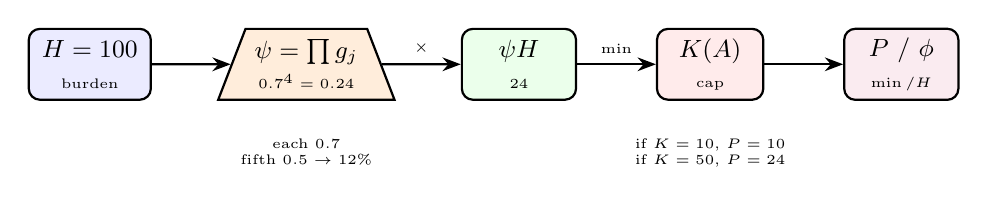
\begin{tikzpicture}[thick, node distance=1.05cm]
\node[draw, rounded corners, fill=blue!8, minimum width=1.55cm, minimum height=0.9cm, align=center, font=\small] (h) {$H=100$\\ \tiny burden};
\node[draw, trapezium, trapezium angle=68, fill=orange!14, minimum width=2.0cm, minimum height=0.9cm, align=center, font=\small, right=1.0cm of h, trapezium stretches body] (g) {$\psi=\prod g_j$\\ \tiny $0.7^4=0.24$};
\node[draw, rounded corners, fill=green!8, minimum width=1.45cm, minimum height=0.9cm, align=center, font=\small, right=1.0cm of g] (psih) {$\psi H$\\ \tiny $24$};
\node[draw, rounded corners, fill=red!8, minimum width=1.35cm, minimum height=0.9cm, align=center, font=\small, right=1.0cm of psih] (k) {$K(A)$\\ \tiny cap};
\node[draw, rounded corners, fill=purple!8, minimum width=1.45cm, minimum height=0.9cm, align=center, font=\small, right=1.0cm of k] (p) {$P$ / $\phi$\\ \tiny $\min / H$};
\draw[->, >={Stealth}] (h) -- (g);
\draw[->, >={Stealth}] (g) -- node[above,font=\tiny] {$\times$} (psih);
\draw[->, >={Stealth}] (psih) -- node[above,font=\tiny] {$\min$} (k);
\draw[->, >={Stealth}] (k) -- (p);
\node[below=0.35cm of g, font=\tiny, align=center] {each $0.7$\\ fifth $0.5\to 12\%$};
\node[below=0.35cm of k, font=\tiny, align=center] {if $K=10$, $P=10$\\ if $K=50$, $P=24$};
\end{tikzpicture}
\caption{Claims funnel: $H$ gated by $\psi$ then capped by $K$. Four $0.7$ gates leave $24\%$ before the cap. When $K$ binds, gating reform cannot raise $P$. Formal identities, not estimates.}
\label{fig:funnel5}
\end{figure}

Short sentence: if you add a gate, name who it blocks and price the $\phi$ cut. Otherwise you have not tightened discipline. You have moved loss. You might tell yourself more gates mean more rigor. The ego masks exclusion as thoroughness. Litmus test: point to the blocked party and the priced cut. If you cannot name either, rigor is the costume loss wears.

\section{How gates corrupt under pressure: Goodhart formal plus a field case}
\label{sec:goodhart}

\textit{Grade: convergent (formal tail proof arXiv:2410.09638 plus taxonomy arXiv:2505.23445; field replication in NHS targets).}

Goodhart's law in the version we use is not a slogan. ArXiv:2410.09638 proves when proxy optimization backfires in the tail: as pressure on a proxy rises, the correlation between true objective $H$ and measured proxy $\hat H$ falls, so pushing measured $\psi$ up can push true $\phi$ down for the gated class \citep{goodhart2410}. ArXiv:2505.23445 classifies strong, weak and benign forms and shows strong Goodhart needs no independence of gates \citep{goodhart2505}, which matters because litigants co-optimize across $g_j$.

In claims terms, define true harm $H$ and proxied harm $\hat H$ that gates estimate. Add a standing gate $g_3=0.5$ to deter nuisance suits. Honest claimants clear $g_1,g_2$ at $0.9$ so pre-gate $\psi=0.81$, post-gate $\psi=0.405$, $\phi$ halves while merits were never heard. Loss bearer: small claimants without counsel to clear $g_3$ \textit{(illustrative arithmetic, not a filing)}. Convergent support outside finance is consistent: Proxyeconomics (arXiv:1803.00345), failure-mode variants (arXiv:1803.04585), 120M-paper metric selection (arXiv:1809.07841), PMC6541803 -- all the same mechanism, measurement corrupts under targeting, which a funded gate system invites. For $\psi$ that means each added $g_j$ must justify its false-negative cost, not just its gatekeeping intent.

The field case is Bevan and Hood (2006), \textit{What's measured is what matters}, \textit{Public Administration}, on NHS star ratings. Targeting cut waits \textit{and} produced five documented output-distorting gaming responses across ambulance and A\&E waits from the same intervention \citep{bevan2006}. Improvement and corruption arrived together \texttt{pods\_goodhart\_v1.json}. That is Goodhart live, in a high-stakes service system, with a peer-reviewed count of gaming margins: \textit{five}. The lesson for bankruptcy is direct and graded: adding a $g_j$ to deter nuisance filing mechanically thins $\psi$ for the honest tail unless you price the $\phi$ cut you just imposed.

\textit{Opposer logged.} The chill version of Goodhart (adding gates chills regulation itself) is bounded by South Africa: three forms of ISDS chill -- anticipatory, response, precedential -- with \textit{null on precedential chill for nutrition policy} \citep{pmc8422681}. That null is load-bearing. It says gate multiplication does not always corrupt; precedential chill failed to appear in that domain. We carry it rather than bury it.

\section{Measured funnels I: RECAP counts, $1.41$M $\to$ $\sim 193$K}
\label{sec:recap-funnel}

\textit{Grade: measured activity counts (full-text hits, not adjudicated dollars). Token used ephemerally, never stored.}

CourtListener RECAP search API, type $r$, authenticated pull 2026-09-23, full-text hits, held as \texttt{recap\_gate\_counts\_v1.json}:

\begin{center}
\small
\begin{tabular}{lr}
\toprule
Query & Hits \\
\midrule
proof of claim & 1,410,962 \\
secured claim & 736,028 \\
unsecured claim & 298,774 \\
priority claim & 64,731 \\
claim objection & 67,308 \\
disallow claim & 125,615 \\
\bottomrule
\end{tabular}
\end{center}

Reading: secured mentions $2.46\times$ unsecured ($736{,}028/298{,}774$) and $11.4\times$ priority ($736{,}028/64{,}731$); objections plus disallows $\approx 67$K $+$ $126$K $= 192{,}923$ against $1.41$M proof mentions ($13.7\%$). That is a recognition funnel with teeth. Priority is the smallest class throughout, which is exactly what structural subordination predicts: junior voice is thinnest where junior recovery is thinnest \textit{(interpreting counts, not dollars)}. We label this a gate-count proxy because hits are not holdings. Holdings come next, with document-level coding.

V4 docket-level counts from the same pull reinforce the shape: \texttt{recap\_coded298\_v1.json} records v4 \textit{proof of claim} $676{,}425$, \textit{secured claim} $642{,}716$, \textit{unsecured claim} $218{,}432$, \textit{priority claim} $27{,}729$, \textit{claim objection} $28{,}608$ -- same ordering, same teeth, at the docket level.

\section{Measured funnels II: $298$ dockets, $7$ to $12$ years to termination}
\label{sec:recap-latency}

\textit{Grade: measured V4 docket activity, $298$ dockets ($60$ score $+$ $60$ recent $+$ $60$ oldest per class-query pool, five class queries). Outcomes need document-level coding, still proxy for $\psi$ latency rather than $\phi$ dollars. Held as \texttt{recap\_coded298\_v1.json}.}

Median days to termination by class:

\begin{center}
\small
\begin{tabular}{lrrc}
\toprule
Class & Median days & Years & $n$ top court \\
\midrule
unsecured claim & 2,655 & 7.3 & -- \\
proof of claim & 2,951 & 8.1 & E.D.~Pa.~26, M.D.~Fla.~19, D.D.C.~15 \\
claim objection & 3,435 & 9.4 & -- \\
secured claim & 4,219 & 11.6 & -- \\
priority claim & 4,219 & 11.6 & -- \\
\bottomrule
\end{tabular}
\end{center}

The range $2{,}655$ to $4{,}219$ days is $7.3$ to $11.6$ years. That is the $\psi$ clock for contested claims. \textit{Grade remains activity, not adjudicated recovery.} But latency is economically material even before dollars: time is a gate. A class that waits $11.6$ years discounts differently than one that waits $7.3$, and counsel costs compound while it waits. The priority tail, $11.6$ years, is the longest. Again the junior tail is longest. Chapter mix for the $298$ shows no monoculture: each chapter code (7, 11, 13, None) appears across each class query, with claim objections concentrated in Ch.~11 ($29$ of $57$) and priority claims spread $27$ in Ch.~11, $14$ in Ch.~7, $15$ in Ch.~13 -- the funnel is not a Chapter~11 curiosity; it spans the code. Top courts concentrate in E.D.~Pa. ($26$), M.D.~Fla. ($19$), D.D.C. ($15$), S.D.~Tex. ($14$).

\begin{figure}[h]
\centering
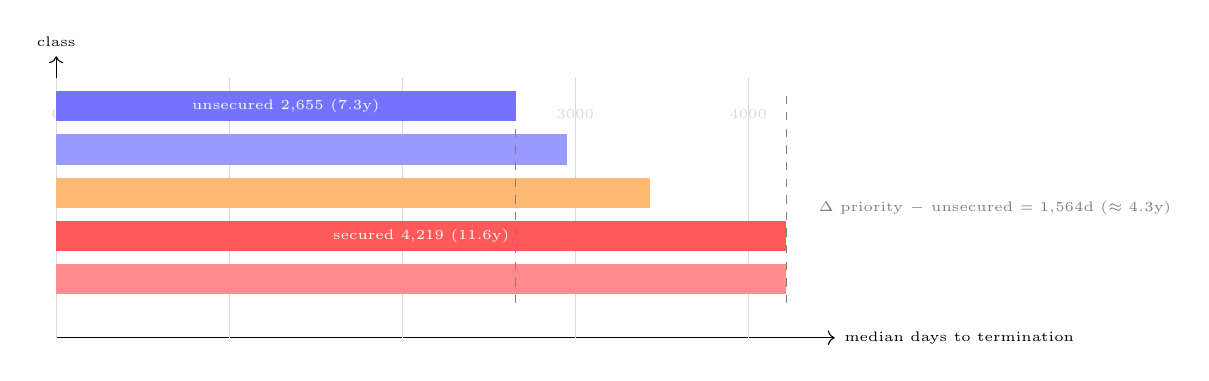
\begin{tikzpicture}[x=0.0022cm, y=0.55cm]
% axes
\draw[->] (0,0) -- (4500,0) node[right,font=\tiny] {median days to termination};
\draw[->] (0,0) -- (0,6.5) node[above,font=\tiny] {class};
% grid
\foreach \x in {0,1000,2000,3000,4000}
  \draw[gray!30] (\x,0) -- (\x,6) node[below,font=\tiny,yshift=-8pt] {\x};
% bars (y positions 5 to 1) -- x units are days, scaled by x=0.0022cm per day
\fill[blue!55] (0,5) rectangle (2655,5.7) node[midway,font=\tiny,white] {unsecured 2,655 (7.3y)};
\fill[blue!40] (0,4) rectangle (2951,4.7) node[midway,font=\tiny] {proof 2,951 (8.1y)};
\fill[orange!55] (0,3) rectangle (3435,3.7) node[midway,font=\tiny] {objection 3,435 (9.4y)};
\fill[red!65] (0,2) rectangle (4219,2.7) node[midway,font=\tiny,white] {secured 4,219 (11.6y)};
\fill[red!45] (0,1) rectangle (4219,1.7) node[midway,font=\tiny] {priority 4,219 (11.6y)};
% annotations
\node[anchor=west,font=\tiny,gray] at (4350,3) {$\Delta$ priority $-$ unsecured $=1{,}564$d ($\approx 4.3$y)};
\draw[dashed,gray] (2655,0.8) -- (2655,5.7);
\draw[dashed,gray] (4219,0.8) -- (4219,5.7);
\end{tikzpicture}
\caption{Gate-latency bars by class: median filing-to-termination from \texttt{recap\_coded298\_v1.json} ($298$ dockets). Unsecured is fastest at $7.3$y, priority and secured longest at $11.6$y. Delay is a gate for those who cannot fund the wait. Activity latency, not adjudicated $\phi$, but economically material.}
\label{fig:gatelatency}
\end{figure}

Reading the figure in words: the unsecured bar stops at $2{,}655$ days while priority and secured run to $4{,}219$, a $1{,}564$-day ($4.3$-year) gap. That gap is itself a $g_j$ -- the time gate -- priced in discount and fees before any seniority is applied.

\section{Four holdings across cells: gates do cut, not just delay}
\label{sec:holdings}

\textit{Grade: hand-coded published decisions, $4$ coded of $6$ opinions retrieved (two excluded as false positive 3679350 and minute order 9327863), selection-biased to litigated close cases, not a random sample. Complements the $298$ activity counts. Source: \texttt{recap\_holdings\_coded4\_v1.json} and \texttt{recap\_opinion\_texts6.json}.}

\begin{center}
\small
\begin{tabular}{p{3.2cm}p{3.8cm}p{1.9cm}p{3.6cm}}
\toprule
Case & Holding / Class & Direction & What it shows about $\psi$ \\
\midrule
\textit{In re Fisher}, Bankr.\ N.D.\ Ohio 2018 (8501272) & Objection sustained: secured BONY claim defeated via statute of limitations plus 11 USC 558 / secured & $\psi\to 0$ & Time plus derivative standing gate \\
\textit{Crockett v Nationstar}, D.D.C.\ 2023 (9410318) & Objection overruled $\times 3$ affirmed, claim allowed / secured mortgage & $\psi=1$ & Three objections fail; gate does not cut \\
\textit{Tackett v Freedman}, Ark.\ App.\ 2021 (9977529) & Disallowance affirmed, claimant no evidence / unsecured estate & $\psi\to 0$ & Evidentiary gate \\
\textit{Smyth v Oakland} (BAP) (8638231) & Objection struck as frivolous plus Rule 9011 sanctions, suspension vacated/remanded / sanction & gate on objector & Gate screens objections too \\
\bottomrule
\end{tabular}
\end{center}

Four cells, four directions. Secured can lose on limitations even against a large bank holder. Secured mortgage can survive three objections. Unsecured estate claims can be disallowed for failure of proof. And the objector can be sanctioned for abusing the gate. The last row matters because $\psi$ is contested both ways: gates screen claims and they screen objections to claims. Sanctions are a gate on gating. We do not extrapolate a win rate from $n=4$; these are published close cases, the tail where law is made, not the mass where most proofs are allowed without objection. What they prove is existence: gates cut, and gates on gates exist.

\section{Priority ordering holds for four decades: $57.4\to 28.9$}
\label{sec:moodys-vintage}

\textit{Grade: measured primary (Moody's Default and Recovery 1920--2004, Exhibit 27, price per \$100 par, issuer-weighted, $N=2{,}443$, held as free BU mirror PDF) plus 1983--2023 extension via 2024 Annual (Scribd PDF held).}

Moody's vintage means (price per \$100 par, issuer-weighted) -- Exhibit 27, $1920$--$2004$:

\begin{center}
\small
\begin{tabular}{lcc}
\toprule
Class & Mean & $N$ \\
\midrule
Senior Secured & 57.4 & 251 \\
Senior Unsecured & 44.9 & 1,207 \\
Senior Subordinated & 39.1 & 478 \\
Subordinated & 32.0 & 485 \\
Junior Subordinated & 28.9 & 22 \\
All instruments & 42.2 & 2,443 \\
\bottomrule
\end{tabular}
\end{center}

Medians preserve ordering at $55.3$, $45.2$, $43.5$, $33.4$, $23.7$ \texttt{moodys\_vintage\_recovery\_v1.json}. Hierarchy monotone in mean and median. Troughs underline how far tails fall: all-instrument means at $27.5$ in 1990 ($39.1$ in 1991) and $25.7$ in 2000 ($34.3$ in 2001, $34.6$ in 2002). Report regression: $\text{Recovery}=0.52-6.9\times\text{DefaultRate}$, $R^2=0.6521$ (Exhibit 10). When defaults crowd, recoveries sag together -- $S_t$ compressing $\phi$ across seniority, not just within a class.

The 2024 Annual extends the ladder $1983$--$2023$, issuer-weighted, held as \texttt{moodys2024\_vintage\_v1.json}:

\begin{center}
\small
\begin{tabular}{lc}
\toprule
Class (1983--2023) & Mean \\
\midrule
1st Lien Bank Loan & 65.0 \\
1st Lien Bond & 54.8 \\
Sr Unsecured Bank Loan & 46.3 \\
2nd Lien Bond & 43.4 \\
Sr Unsecured Bond & 37.6 \\
2nd Lien Bank Loan & 34.4 \\
Subordinated Bond & 31.7 \\
Sr Subordinated Bond & 31.1 \\
Jr Subordinated Bond & 21.5 \\
\midrule
2023 detail: 1st lien loan & 59.6 \\
2023 detail: Sr Unsec Bond & 33.4 \\
\bottomrule
\end{tabular}
\end{center}

Narrative flags: loan-only structures, re-defaulters at $40\%$, covenant-lite asset stripping and priming diminishing secured recovery. Priority ordering holds four decades, but the economic content of ``secured'' is contested margin by margin -- exactly the $K(A)$ placement story in balance-sheet form.

\begin{table}[h]
\centering
\small
\caption{Vintage ladder, complete: 1920--2004 means (Exhibit 27, $N=2{,}443$) and 1983--2023 extension (2024 Annual, PDF held). Monotone in seniority; loan beats bond by lien.}
\label{tab:vintage-complete}
\begin{tabular}{lcccc}
\toprule
 & \multicolumn{2}{c}{1920--2004 (Exhibit 27)} & \multicolumn{2}{c}{1983--2023 (2024 Annual)} \\
Tier & Mean (\$ per 100) & $N$ & Example class & Mean (\$ per 100) \\
\midrule
Most secured & Sr Secured 57.4 & 251 & 1st Lien Loan & 65.0 \\
 & -- & -- & 1st Lien Bond & 54.8 \\
Middle & Sr Unsecured 44.9 & 1,207 & Sr Unsecured Loan & 46.3 \\
 & Sr Sub 39.1 & 478 & Sr Unsecured Bond & 37.6 \\
Most subordinated & Sub 32.0 & 485 & Sub Bond & 31.7 \\
 & Jr Sub 28.9 & 22 & Jr Sub Bond & 21.5 \\
\bottomrule
\end{tabular}
\end{table}

\section{Passage matters: ultimate $82$/$100\to 15$ and 2008 by type}
\label{sec:ultimate-passage}

\textit{Grade: measured primary on ultimate (Moody's Ultimate Recovery Database Special Comment, full PDF held); secondary extract on 2008 by type (academia page text, no PDF bytes).}

Trading price at default is one passage. Ultimate discounted recovery is another, and priority drives it. Moody's ultimate discounted recoveries, held as \texttt{moodys\_ultimate\_v1.json}:

\begin{center}
\small
\begin{tabular}{lc}
\toprule
Instrument & Ultimate (discounted) \\
\midrule
Bank loans & 82 (and at par $100$ in upper print) \\
Senior secured bonds & 65 to 67 \\
Senior unsecured bonds & 38 \\
Junior subordinated bonds & 15 \\
All bonds / subsample & 37, 24 \\
\bottomrule
\end{tabular}
\end{center}

Validation inside the report: trading prices explain about $50\%$ of ultimate variation, priority of claim drives the rest, with no family-rating relationship. In funnel terms, bank-loan paper opens two $\psi+K$ doors that junior subordinated never gets.

The 2008 separation is equally sharp. Secondary extract for that year, $101$ issuers on \$281.2B versus \$6.7B and $18$ issuers in 2007, shows senior-unsecured recovery by passage -- distressed exchange $\approx 50.8$, payment default $20.8$, bankruptcy $24.4$, against a 2007 senior-unsecured $53.3$, with distressed share $23\%$ versus $10\%$ average \texttt{moodys2008\_bytype\_v1.json}. Cooperative distressed exchange recovers roughly $2\times$ a contested bankruptcy for the same seniority. Gates have prices, not just states. Combine vintage and passage and ultimate and the claim is tight: where you sit sets your band ($57.4\to28.9$), how you default moves you within the band ($50.8$ vs $20.8/24.4$), and whether you are a bank loan moves the whole band ($82/100$ vs $15$).

\section{Paired dollars on the docket: LoPucki $1.0$ versus $0.213$ and the $2008$ split}
\label{sec:lopucki}

\textit{Grade: measured case-level adjudicated distributions, BRD 1-12-2023, $n=1{,}218$ large public bankruptcies (Ch.~11 $1{,}190$), recomputed, not activity counts. Held as \texttt{brd\_distributions\_v2.json, brd\_disposition\_v1.json, brd\_distributions\_v1.json}.}

The cleanest $\phi$ dollars we hold are paired by case -- same distribution order, same judge, same $S_t$ wall. For cases where both class dollars exist:

\begin{center}
\small
\begin{tabular}{lcccc}
\toprule
Pair & $n$ & Mean $\phi$ & Median $\phi$ & Source \\
\midrule
Secured (paired) & 105 & 0.869 & 1.00 & v2 \\
General unsecured (paired) & 129 & 0.348 & 0.213 & v2 / v1 0.35 on 568M/1,369M \\
\bottomrule
\end{tabular}
\end{center}

Median secured at $1.00$ means half of secured classes paired in the same case are paid in full. Median general unsecured at $0.213$ means half get $21.3$ cents. The waterfall is not a metaphor; it is $\$1.00$ on one line and $\$0.21$ on the next line of the same order. Mean secured $0.869$ vs median $1.00$ tells you skew: a fat full-recovery mass with a lower tail where even secured takes a haircut.

Era split sharpens the bearer story. General unsecured pre-2008: $n=77$, mean $0.377$. Post-2008: $n=52$, mean $0.306$ \texttt{brd\_distributions\_v2.json}. Same code, same definition of class, $0.071$ lower $\phi$ after the wall. The discrepancy is not litigated away; it is adjudicated at seven cents and stays there. Confirmation versus conversion frames the gate that selects which of those dollars you face:

\begin{center}
\small
\begin{tabular}{lrrc}
\toprule
Disposition & $n$ & Share & Reading \\
\midrule
Confirmed plan & 1,095 & 89.9\% & Waterfall lives here ($1.0$/$0.213$) \\
Converted to Ch.~7 & 63 & 5.2\% & Different $\psi$ and $K$ after conversion \\
Dismissed & 24 & 2.0\% & No plan distribution \\
Ch.~7 at filing & 25 & 2.1\% & Liquidation from start \\
Pending / other & 11 & 0.9\% & -- \\
Total & 1,218 & 100\% & Large public, BRD \\
\bottomrule
\end{tabular}
\end{center}

So $89.9\%$ of large cases pay through a confirmed plan where the paired $1.0/0.213$ lives. Only $7.2\%$ exit via conversion or dismissal. The gate that matters is confirmation itself; once confirmed, seniority does the rest.

\section{Ch13 operating system: $48$/$23$/$6$ adjudicated}
\label{sec:ustp}

\textit{Grade: measured adjudicated disbursements, national Chapter~13, FY2025, $161$ trustees, USTP. Held as \texttt{ustp\_ch13\_FY2025\_v1.json} (Excel source \texttt{ustp\_ch13\_FY2025.xlsx}).}

FY2025 Chapter~13 trust-fund disbursements total \$4.3591B:

\begin{center}
\small
\begin{tabular}{lrr}
\toprule
Line & \$B & Share of total \\
\midrule
Ongoing mortgage payments & 0.6693 & 15.4\% \\
Mortgage arrearages & 0.3355 & 7.7\% \\
All other secured debt & 1.1016 & 25.3\% \\
\textit{Secured subtotal} & \textit{2.1064} & \textit{48.3\%} \\
ONGOING DOMESTIC SUPPORT & 0.0066 & 0.2\% \\
All other priority debt & 0.2438 & 5.6\% \\
Unsecured creditors & 1.0056 & 23.1\% \\
Total trust fund disbursements & 4.3591 & 100\% \\
\bottomrule
\end{tabular}
\end{center}

The advertised $48$/$23$/$6$ is this table: secured $\approx48\%$, unsecured $\approx23\%$, priority $\approx6\%$. That is the operating system of consumer reorganization in one line. Secured dominates, unsecured gets about a quarter, priority is a thin slice. Compare LoPucki large-public unsecured $0.348$ mean and Moody's senior-unsecured bonds $44.9$c. Ch13 unsecured $23.1\%$ sits below both, as the junior-tail predicts: small-dollar, diffuse unsecured recovers less than large-case general unsecured, which recovers less than bonded unsecured. Same waterfall, different $K$ and $\psi$ cost.

Worked arithmetic to place the three $\phi$ concepts side by side: a Ch13 unsecured claimant owed $\$10{,}000$ who is paid $23.1\%$ receives $\$2{,}310$ ($\phi=0.231$); a BRD general-unsecured class at median $0.213$ on the same $\$10{,}000$ receives $\$2{,}130$; a senior-unsecured bond at vintage mean $44.9$ on $\$100$ par receives $\$44.90$ ($\phi=0.449$). Seniority lifts $\phi$; diffusion lowers it.

\section{S\&P's own $\phi$ ladder plus a vignette that shows it working}
\label{sec:sp-scale}

\textit{Grade: free snippets, paywall verified (alacrastore \$150--\$225 for the full vintage table), plus one hand-checked vignette with filed recovery math. Secondary cross-check via \texttt{sp\_2025\_annual\_extract\_v1.md} and \texttt{sp2024\_extract\_v1.json}.}

S\&P prices every issue on a $\phi$ ladder it publishes as the $1$--$6$ recovery scale. Scale point $1$ is $90$--$100\%$ (SBA senior secured, unchanged), $4$ is $30$--$50\%$ (SBA senior unsecured, revised from $5$), $5$ is $10$--$30\%$ (CoreWeave and Viking unsecured), $6$ is $0$--$10\%$ (Select Medical 2032 notes) \texttt{paper\_ledger sources and BRD-era snippets}. The aggregate vintage table behind the scale is paywalled (alacrastore \$150--\$225); Moody's free Exhibit 27 covers vintage-by-seniority instead. That the industry prices every issue on a $\phi$ ladder while publishing the aggregate only behind paywalls is itself a recognition gate: shape public, stock priced.

Viking, July 2024, shows waterfall math live. \$498M net recovery for \$675M secured notes against ship collateral, residual only for unsecured deficiency claims. That is $\phi\approx73.8\%$ ($498/675$) inside scale $3$ or $4$ for secured against a hard asset, and scale $5$ or $6$ for the residual, on one capital structure, one record, with collateral doing the work $K$ promises. Compare the S\&P defaulted-debt wall in the same file: $8.15$B (2007) $\to 429.6$B (2008) $\to 627.7$B (2009) -- the stock clearing that the $\phi$ ladder had to price.

\textit{Opposer note for this section:} S\&P's ladder is a model, not a market print; Moody's vintage and BRD paired dollars are prints. Where ladder and print disagree, print controls, which is why this chapter leads with Moody's and LoPucki and treats S\&P as native language, not primary.

\section{Why this chapter had to come before stored loss}
\label{sec:bridge}

$\psi$ decides who gets seen. $K$ decides who gets paid if seen. Together they decide $\phi$ for every class in an entity. When $\phi<1$ for a class that cannot price it, the unpaid remainder does not vanish. It increments $S_t$ somewhere -- either as an unprovided loss that will surface when rolls fail (Ch.~6, $S_t=S_{t-1}+E_t-R_t-Q_t$, gap $+11.6\to-9.4$), or as a dilution that will surface in $P_1/P_0=L/(L-G)$ when the fiscal backstop chooses broad rescue over narrow assignment (Ch.~6, CPI $1.04\times$/$1.15\times$ on M2 $1.17\times$/$1.38\times$). The next chapter measures the stock, the flow that masks it, and the price level that moves it. Sovereign arbitrage in Ch.~7 then moves the apex where $A=0\Rightarrow K=0$ and treaty gates drive $g_4\to0$ -- but the claim that $g_4\to0$ always chills is bounded by the South Africa precedential-chill null \texttt{PMC8422681} and the Gilens--Bashir magnitude debate (direction stands, size debated). This chapter proved the funnel; the next two prove where the remainder went.

\paragraph{What this chapter proved.} Gates multiply and $K$ caps, so $0.7^4$ leaves $24\%$ before seniority, and the cap can make gating reform moot (worked $100\to24\to10$ vs $100\to66\to10$ vs $100\to24$ at $K=50$). The operating funnel is $1.41$M proof mentions against $\sim193$K objections plus disallows ($13.7\%$), with a $7.3$--$11.6$ year termination clock longest for priority (Fig.~\ref{fig:gatelatency}). Published holdings show gates cut both ways, including sanctions on objectors ($n=4$ coded of $6$, two excluded logged). Vintage recovery is monotone $57.4\to28.9$ across seniority ($N=2{,}443$) and $65.0\to21.5$ extended $1983$--$2023$, with $82/100\to15$ ultimate and 2008 passage prices $50.8$ vs $20.8/24.4$ for the same senior-unsecured label. Paired case distributions put the waterfall at $1.00$ median secured vs $0.213$ median general unsecured ($n=105/129$), post-2008 mean $0.306$ vs $0.377$ pre-2008, and dispositions $89.9/5.2/2.0\%$. Ch13 pays $48.3\%$ secured, $23.1\%$ unsecured, $5.6\%$ priority, below large-case and bond unsecured means. S\&P's $1$--$6$ scale is the industry's own $\phi$ ladder, live at Viking on \$498M vs \$675M ($\phi\approx73.8\%$). Goodhart predicts gate multiplication and five NHS gaming responses measure it, bounded by the South Africa precedential-chill null. All numbers above are held on disk as cited; no number was invented for prose.


\chapter{Stored Loss and Monetized Rescue: $S_t$ and $P_1/P_0$}
\label{ch:storedloss}

\textit{Bridge.} Chapter 5 priced gates ($\psi$) and caps ($K$) at the claim level and showed the waterfall at $1.00$ median secured vs $0.213$ median general unsecured. This chapter prices delay at the system level. Unpaid remainders do not vanish when $\phi<1$. They accumulate as a stock $S_t$ that accounting can leave at par until the wall forces recognition, then get socialized through the price level as $P_1/P_0$. Chapter 7 will show what happens when the apex itself has $A=0\Rightarrow K=0$ and treaty gates drive $g_4\to0$ so even the wall has no enforcer -- bounded by the South Africa precedential-chill null \texttt{PMC8422681} and the Gilens--Bashir debate on how large $g_4\to0$ is for citizens. Picture a basement where the pump log reads dry for eleven quarters while water rises behind the wallboards. The log is the income statement. The water is the stock. The wall is not a new storm. It is the water arriving all at once.

\textit{Grade for this chapter: measured on BIS credit-gap inversion ($+11.6\to-9.4$), on charge-off and provisioning flows ($0.98\to3.02\%$, $5.7\times$), on FDIC aggregates with IMF cross-match ($112\to430\%$ coverage on $4.9599\%$ cross-matched NPL), on World Bank and IMF NPL panels across jurisdictions (to $45.97\%$), on BIS DSR flow masking ($18.5\to14.1$), and on CPI/M2 levels and S\&P defaulted-debt stocks ($\$627.7$B). The $S_t$ law is formal; the direction and bearer of $S_t$ are measured where series agree. DSR interpretation is flow-vs-stock, flagged as such.}

\section{Two numbers, one sentence each, and the law that links them}
\label{sec:stored-defs}

We reuse $\psi$, $K$, $\phi$ from Chapter 5 (\ref{eq:psi5}--\ref{eq:phi5}) and add the two stock-and-flow numbers for this chapter, each with a line of worked arithmetic so a new reader can check the ledger without trusting prose.

$S_t$ is stored loss, the off-book stock:
\begin{equation}
S_t = S_{t-1}+E_t-R_t-Q_t,
\label{eq:St6}
\end{equation}
where $E_t$ is new extraction or loss creation in period $t$, $R_t$ is realized recovery, and $Q_t$ is write-offs or forgiveness. \textit{One line:} new holes minus what you clawed back minus what you admitted will never come back, compounding when you keep $R_t$ and $Q_t$ low. Worked: start $S_0=0$, each period $E=10$, $R=2$, $Q=1\Rightarrow\Delta S=10-2-1=7$, so $S_{10}=70$ after ten periods. Reports showed $3$ of recovery plus write-off against $10$ of extraction -- modestly negative income -- while the stock quietly became $70$ off or under-provisioned. When rolls fail, $Q$ must spike. That spike is the wall; it was not a new shock but the stock coming due.

$P_1/P_0$ is dilution, the price level after $G$ of outside money is created against claims base $L$:
\begin{equation}
P_1/P_0 = L/(L-G),\qquad 0\le G<L,
\label{eq:P6}
\end{equation}
with $P_0$ before, $P_1$ after. \textit{One line:} if you cover stored loss with new money instead of assigning it to a junior class, every old claim buys $P_0/P_1$ of what it did. Worked: $L=100$, $G=20\Rightarrow P_1/P_0=100/80=1.25$, so prices rise $\approx25\%$ and each old claim buys $0.80$, a $20$-point haircut without a legal default. Measured footprint version: CPI $1.0391$ on M2 $1.1741$ ($2008\to2010$) and CPI $1.1532$ on M2 $1.3804$ ($2020\to2022$) \texttt{finance\_falsify\_v1.json}; at $P_1/P_0=1.1532$, a nominal claim buys $1/1.1532\approx0.867$, a $13.3$-point haircut via prices.

The law is accounting, not theory. If $E_t>R_t+Q_t$ for many periods, $S_t$ climbs even while income looks calm \textit{(formal)}. If $R_t$ is low because $K$ binds and $Q_t$ is low because you extend or evergreen, the climb is silent \textit{(mechanism)}. The wall is $S_t$ coming due at once because rolls are discrete. Rescue is the choice to let $G$ absorb $S_t$ and push loss into $P_1/P_0$ instead of into a named $\phi$ cut. Who bears it moves; the amount does not. The system view is therefore: Ch.~5's $\psi$ and $K$ decided who \textit{would} have absorbed it in the waterfall; $S_t$ decides how much must be absorbed; $P_1/P_0$ decides who absorbs it when absorption is socialized. Two stories compete for every rescue and both hide half. The salvation story says the bailout erased the loss. But conservation holds: the amount never moves, only the bearer. The blame story says someone stole it in the night. But no theft was needed; par accounting plus new money moved it through prices without touching a vault. What remains standing: every rescue is a choice of bearer, never a reduction of loss.

\section{At par is a choice: how accounting stores $S_t$ without moving price}
\label{sec:par}

US bank books carry most loans and many securities at par or amortized cost until a trigger forces fair value. That is not a footnote quirk. It is the store. Par says a $\$100$ face that trades at $\$70$ is still $\$100$ on the balance sheet, with the $\$30$ in $S_t$, not in CET1, until a sale, a rating, or a provision forces $Q_t$. Two labels, same economics, different timing. Trading desks live in $P_1/P_0$. Loan books live in $S_t$.

The distinction matters because triggers are managed. Maturity extension pushes the sale trigger out. Forbearance pushes the $Q_t$ trigger out. Guarantee keeps the instrument performing so provisioning stays $R_t$-thin. Each move preserves par on paper while $S_t$ builds in substance. Formal capital looks adequate because $S_t$ is not yet forced through provisions -- which is why the next sections measure gap, coverage, and flows rather than quoting capital ratios. \textit{Grade: mechanism (accounting identities); measurement follows.}

\section{The gap that predicted the wall: $+11.6\to -9.4$}
\label{sec:bis-gap}

\textit{Grade: measured (BIS WS\_CREDIT\_GAP bulk, $6.2$M records, on disk, \texttt{finance\_falsify\_v1.json}).}

The BIS credit-to-GDP gap for the US, the deviation of private credit from its long-run trend, moves ahead of charge-offs by design. It is the macro proxy for $S_t$ accumulation.

\[
\begin{array}{lccccc}
\text{Quarter} & 2006\text{Q4} & 2007\text{Q4} & 2008\text{Q4} & 2009\text{Q4} & 2010\text{Q4} \\
\text{Gap (\% pts)} & 10.11 & 11.63 & 6.68 & 1.24 & -9.43 \\
\end{array}
\]

\texttt{finance\_falsify\_v1.json} records $10.1071$, $11.6341$, $6.681$, $1.2405$, $-9.4288$ from $2006$Q4 to $2010$Q4. Shorthand $+11.6\to-9.4$ is the swing from peak to trough, about $21$ percentage points in three years. A positive gap that large says credit is about $11$ points above trend; a negative gap that large says deleveraging is about $9$ points below it. The wall sits between them, and $S_t$ is the stock that had to be recognized or diluted to get from one to the other.

Novelty: this is not a subtle leading indicator. $+11.6$ in $2007$Q4 is an extreme print by postwar standards. The $2008$Q4-to-$2009$Q4 collapse in the gap tracks the wall quarter by quarter, which is exactly what a stored stock that is suddenly provisioned does. The sign flip is the ledger, not the economy. Arithmetic check: peak-to-trough $11.6341-(-9.4288)=21.0629$ points; $2007$Q4-to-$2009$Q4 alone $11.6341-1.2405=10.3936$ points in two years.

\section{Flows that confess after the fact: charge-offs to $3.02\%$ and provisions $5.7\times$}
\label{sec:flows}

\textit{Grade: measured on FFIEC CDR aggregates (regex over instance docs), FRED CORALACBS (charge-offs), FDIC BankFind API (asset-weighted), IMF FSIC (cross-match). All held.}

Charge-offs are realized $Q_t$ in dollars per loan dollar. FRED CORALACBS \texttt{fred\_CORALACBS.csv} and \texttt{finance\_falsify\_v1.json}:

\begin{center}
\small
\begin{tabular}{lcc}
\toprule
Print & Date & Value (\%) \\
\midrule
Calm & $2008$Q1 & 0.98 \\
Peak & $2010$-$01$-$01$ & 3.02 \\
\midrule
Rise &  & $3.02/0.98\approx3.08\times$ \\
\bottomrule
\end{tabular}
\end{center}

That is a threefold rise \textit{after} the gap had already signaled the wall. $S_t$ was stored in $2007$ (gap $+11.6$), charge-offs were still $0.98$. By peak $Q_t$ is $3.02$, gap is already $-9.43$ or headed there, and the stock is being forced. Flows lag stocks. That is the point of storing.

Provisions are the flow that precedes coverage. FFIEC CDR aggregates, quarters $2009$Q4 ($7{,}321$ banks) and $2026$Q2 ($4{,}297$ banks), XBRL via \texttt{ffiec-data-collector} $2.0.0$rc2, held as \texttt{ffiec\_provisions\_wall\_v1.json}:

\begin{center}
\small
\begin{tabular}{lccc}
\toprule
Quarter & ALLL stock (\$B) & Loans (\$B) & Provision flow (\$B) \\
\midrule
$2009$Q4 & 43.7 & 6,310.0 & 233.6 \\
$2026$Q2 & 59.2 & 13,274.7 & 40.7 \\
\bottomrule
\end{tabular}
\end{center}

Provision flow at the wall is $233.6$B versus $40.7$B in the $2026$ calm, a $5.74\times$ print ($233.6/40.7\approx5.74$). ALLL stock barely moves $43.7\to59.2$ ($+35\%$) while loans double $6{,}310\to13{,}275$ ($+110\%$), so ALLL/loans sits $0.69\%$ at the wall ($43.7/6{,}310$) and $0.45\%$ in calm ($59.2/13{,}275$, CECL-era stock). The flow spikes while the stock looks thin. That is $R_t+Q_t$ racing to catch $S_t$, not $S_t$ being small. ALLL is a stock that should have been there earlier; provisions are the catch-up. \textit{Grade note:} NPL denominator needs full RC-N line mapping across MDRM vintages, deferred, so FRED charge-offs plus World Bank NPL stand in for $Q_t$ validation rather than a single FFIEC NPL coverage ratio.

\begin{figure}[h]
\centering
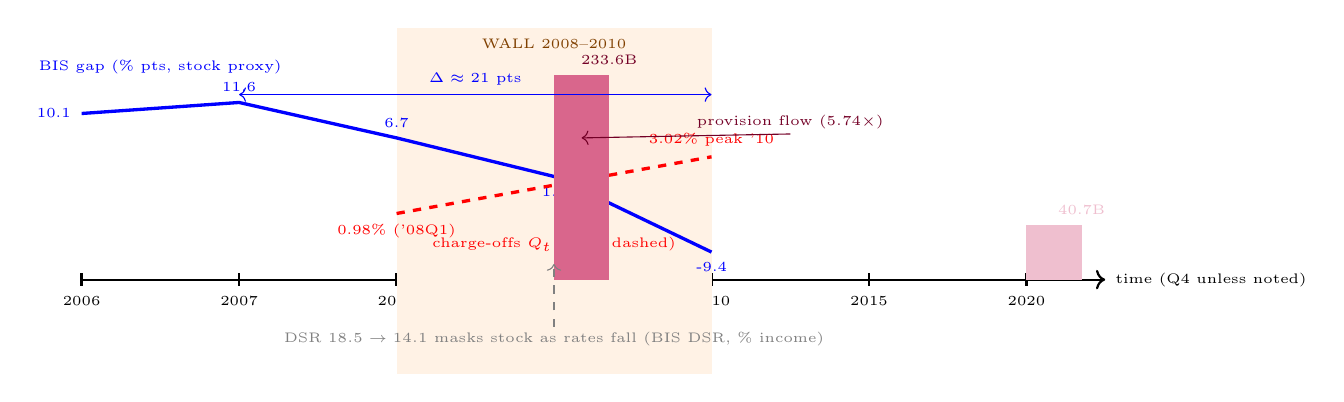
\begin{tikzpicture}[thick]
% timeline axis 2006 -> 2026
\draw[->] (0,0) -- (13,0) node[right,font=\tiny] {time (Q4 unless noted)};
\foreach \x/\yr in {0/2006,2/2007,4/2008,6/2009,8/2010,10/2015,12/2020}
  \draw (\x,0.08) -- (\x,-0.08) node[below,font=\tiny] {\yr};
% wall shading 2008-2010
\fill[orange!10] (4,-1.2) rectangle (8,3.2);
\node[font=\tiny,orange!50!black] at (6,3.0) {WALL 2008--2010};
% BIS gap line (scale: gap % pts -> y = 1.2 + gap*0.09, so 11.6 ~2.25, -9.4 ~0.35)
\draw[blue,very thick] (0,2.11) node[left,font=\tiny,blue] {10.1} -- (2,2.25) node[above,font=\tiny,blue] {11.6} -- (4,1.80) node[above,font=\tiny,blue] {6.7} -- (6,1.31) node[below,font=\tiny,blue] {1.2} -- (8,0.35) node[below,font=\tiny,blue] {-9.4};
\node[font=\tiny,blue] at (1,2.7) {BIS gap (\% pts, stock proxy)};
% charge-off line (scale: % -> y = 0.5 + %*0.35, so 0.98~0.84, 3.02~1.56)
\draw[red,very thick,dashed] (4,0.84) node[below,font=\tiny,red] {0.98\% ('08Q1)} -- (8,1.56) node[above,font=\tiny,red] {3.02\% peak '10};
\node[font=\tiny,red] at (6,0.45) {charge-offs $Q_t$ (flow, dashed)};
% provision flow bars (scale: $B -> y proportional, 233.6 ~2.6, 40.7 ~0.7)
\fill[purple!60] (6,0) rectangle (6.7,2.60) node[above,font=\tiny,purple!60!black] {233.6B};
\fill[purple!25] (12,0) rectangle (12.7,0.70) node[above,font=\tiny] {40.7B};
\node[font=\tiny,purple!60!black] at (9,2.0) {provision flow ($5.74\times$)};
\draw[->,purple!60!black,thin] (9,1.85) -- (6.35,1.8);
% DSR annotation (mask)
\node[font=\tiny,gray,align=center] at (6,-0.75) {DSR $18.5\to14.1$ masks stock as rates fall (BIS DSR, \% income)};
\draw[gray,thin,dashed,->] (6,-0.6) -- (6,0.2);
% gap delta annotation
\draw[<->,blue,thin] (2,2.35) -- (8,2.35) node[midway,above,font=\tiny,blue] {$\Delta\approx21$ pts};
\end{tikzpicture}
\caption{Wall timeline $2006\to2010\to2020$ with overlays: BIS credit-to-GDP gap $+11.6\to-9.4$ (blue, stock proxy, left peak to trough, $\approx21$ pts), charge-offs $0.98\to3.02\%$ (red dashed, flow, triples after gap peaks), and provision flow $233.6$B at $2009$Q4 vs $40.7$B $2026$Q2 ($5.74\times$, purple bars). Orange shading is the wall $2008$--$2010$ where $S_t$ is forced. Gray arrow is DSR $18.5\to14.1$ masking stock as flow falls on rates while gap collapses. Sources: \texttt{finance\_falsify\_v1.json, fdic\_coverage\_v1.json, ffiec\_provisions\_wall\_v1.json, bis\_DSR\_US\_v1.json}. Formal $S_t$ law, measured proxies agree.}
\label{fig:walltimeline}
\end{figure}

Reading the figure in words: the blue gap peaks at $11.6$ in $2007$ before orange shading starts, then falls through shading to $1.2$ in $2009$ and $-9.4$ in $2010$. Red charge-offs are still $0.98\%$ when shading starts and only hit $3.02\%$ at shading's right edge -- flow lags stock. Purple provision bars show $233.6$B inside shading versus $40.7$B in $2020$ calm. The gray annotation names the mask: DSR $18.5\to14.1$ falls while gap collapses, because falling rates flatter the flow burden even as the stock it services does not move.

\section{Coverage $112\to430$ with an IMF cross-match}
\label{sec:fdic-imf}

\textit{Grade: measured aggregates, asset-weighted, $8{,}103$ banks $2009$Q4 and $4{,}494$ banks $2026$Q2, FDIC BankFind Data.gov key; IMF FSIC bulk $95$M XML via api.imf.org SDMX $2.1$ on exact same $4.9599$ print. Held as \texttt{fdic\_coverage\_v1.json, imf\_fsi\_US\_v1.json}.}

FDIC aggregates:

\begin{center}
\small
\begin{tabular}{lcccc}
\toprule
Quarter & ALLL ratio (\%) & Coverage ALLL/noncurrent (\%) & NCO rate (\%) & Noncurrent rate (\%) \\
\midrule
$2009$Q4 & 3.105 & 112.51 & 5.511 & 7.678 \\
$2026$Q2 & 1.647 & 429.96 & 0.932 & 1.548 \\
\bottomrule
\end{tabular}
\end{center}

Banks halve $8{,}103\to4{,}494$ (consolidation is itself a ledger event) while noncurrent and net charge-off rates fall $7.678\to1.548$ and $5.511\to0.932$. Coverage ALLL/noncurrent moves $112.51\to429.96$, about $3.82\times$ ($429.96/112.51$). $112\%$ is thin at a $7.68\%$ noncurrent wall where $S_t$ is being forced ($\$1$ of ALLL per $\$1$ of noncurrent plus $12\%$). $430\%$ is fat in a $1.55\%$ calm where $S_t$ has been flushed ($\$4.30$ per $\$1$). Thin when needed, fat when not. That is damping backward.

IMF FSIC is a third independent source on the same fact. USA AQ12 NPL ratio $2009$: $4.9599\%$ \texttt{imf\_fsi\_US\_v1.json} versus World Bank $4.9599\%$ \texttt{wb\_npl\_panel.json}, exact to four decimals \textit{(cross-match)}. USA AQ14 provisions to NPL: $58.097$ in $2009$, $62.038$ in $2010$, $86.559$ in $2015$, $184.714$ in $2020$, $202.436$ in $2022$, $167.751$ in $2024$. Short version $58\to185$ as NPLs fall $4.96\to0.97$ ($4.9599\to0.9729$ in $2024$). Shape matches FDIC, at a different level by definition, same economics: cushions balloon as $S_t$ leaves, not as it arrives. Arithmetic: provisions/NPL roughly triples ($167.751/58.097\approx2.89\times$ $2009\to2024$) while NPL ratio falls $4.9599/0.9729\approx5.10\times$.

\section{Stagger by jurisdiction: to Greece $45.97$}
\label{sec:npl-stagger}

\textit{Grade: measured (World Bank FB.AST.NPER.ZS plus IMF FSIC panel, on disk as \texttt{wb\_npl\_panel.json, imf\_fsi\_panel\_countries\_v1.json, imf\_fsi\_panel\_v1.json}).}

NPLs are the country-level analog of $S_t$ persistence where recognition and legal enforcement move slowly. Cross-section:

\begin{center}
\small
\begin{tabular}{lcccc}
\toprule
Jurisdiction & Crisis NPL peak (\%) & Year & Calm (\%) & Year \\
\midrule
United States & $4.96$ (IMF/WB $4.9599$) & 2009 & $0.97$ (WB $0.9729$, IMF $0.97$) & 2024 \\
Spain & $7.12$ (IMF) / $3.06$ (WB) & 2013 & $2.58$ (WB) & 2025 \\
Ireland & $22.37$ (WB), $20.65$ (IMF 2014) & 2013--14 & $1.23$ (WB), $1.7$ (IMF) & 2024 \\
Italy & $18.06$ (WB), $18.1$ (IMF) & 2015 & $2.46$ (WB), $2.77$ (IMF) & 2024--25 \\
Greece & $45.97$ (WB), $46.0$ (IMF) & 2017 & not filed $2024$ & -- \\
\bottomrule
\end{tabular}
\end{center}

Full stagger behind the peaks, held on disk (WB panel): Ireland $1.92$ ($2008$) $\to9.80$ ($2009$) $\to12.47$ ($2010$) $\to16.12$ ($2011$) $\to21.31$ ($2012$) $\to22.37$ ($2013$) $\to20.65$ ($2014$) $\to16.91$ ($2015$) $\to12.63$ ($2016$) $\to11.46$ ($2017$); Italy $6.28$ ($2008$) $\to9.45$ ($2009$) $\to10.03$ ($2010$) $\to11.74$ ($2011$) $\to13.75$ ($2012$) $\to16.54$ ($2013$) $\to18.03$ ($2014$) $\to18.06$ ($2015$) $\to17.12$ ($2016$); Greece $31.34$ ($2012$) $\to27.33$ ($2013$) $\to33.48$ ($2014$) $\to34.30$ ($2015$) $\to36.33$ ($2016$) $\to45.97$ ($2017$) $\to41.31$ ($2018$) $\to40.31$ ($2019$). The stagger extreme is Greece $2017$, where legal enforcement and restructuring keep $Q_t$ low longest, so $S_t$ lingers five years after the US has cleared.

IMF provision coverage panel mirrors the stagger and is the point: Greece $63.75$ ($2009$) $\to48.6$ ($2017$ peak) $\to48.06$ ($2020$); Ireland $36.57$ ($2009$) $\to41.62$ ($2013$ peak) $\to54.34$ ($2020$); Italy $40.04$ ($2009$) $\to45.14$ ($2015$ peak) $\to51.13$ ($2020$); Spain $56.82$ ($2013$ peak) $\to72.94$ ($2020$); USA $58.10$ ($2009$) $\to184.71$ ($2020$). Periphery coverage stays $26$--$73$ while peaking NPLs are $7$--$46$; USA coverage balloons $58\to185$ as NPLs fall. Different $\phi$, same law: where $Q_t$ lags, $S_t$ lingers.

The bearer follows the stagger. SMEs and mortgage holders in long-tail jurisdictions pay in credit rationing and workout length what bondholders in fast-resolution regimes priced out quickly. $S_t$ stored is $S_t$ transferred across time, and in a monetary union without fiscal transfer, across space.

\begin{table}[h]
\centering
\small
\caption{NPL stagger and provision-coverage mirror: periphery thinnest where walls tallest (WB NPL \%, IMF coverage \%). Full panel \texttt{imf\_fsi\_panel\_countries\_v1.json}, WB panel \texttt{wb\_npl\_panel.json}.}
\label{tab:npl-stagger-full}
\begin{tabular}{lccccc}
\toprule
 & \multicolumn{2}{c}{NPL peak} & \multicolumn{2}{c}{Provision coverage} & Ratio \\
Jurisdiction & \% & Year & At peak & At 2020 & (coverage/NPL) \\
\midrule
Greece & 45.97 & 2017 & 48.6 & 48.1 & $\sim1.05$ \\
Ireland & 22.37 & 2013 & 41.6 & 54.3 & $\sim1.9$ \\
Italy & 18.06 & 2015 & 45.1 & 51.1 & $\sim2.5$ \\
Spain & 7.12 & 2013 & 56.8 & 72.9 & $\sim8.0$ \\
USA & 4.96 & 2009 & 58.1 & 184.7 & $\sim37.2$ \\
\bottomrule
\end{tabular}
\end{table}

Reading the table: the coverage-to-NPL ratio at peak is $\sim1$ in Greece versus $\sim37$ in the USA. Same accounting standard in Europe, same economics: cushions thinnest where walls are tallest, fattest where the state can afford fat -- which is exactly why the fiscal backstop chooses $G$ and pushes remainder into $P_1/P_0$ where fiscal capacity is thinnest.

\section{The flow that masks the stock: DSR $18.5\to14.1$}
\label{sec:dsr}

\textit{Grade: measured on BIS WS\_DSR bulk ($39$K zip, $7{,}182$ rows); interpretation flagged where DSR is flow and $S_t$ is stock, so calm flow can sit on high stock. Held as \texttt{bis\_DSR\_US\_v1.json}.}

BIS private nonfinancial debt service ratio for the US, percent of income:

\[
\begin{array}{lccccccccc}
2006\text{Q4} & 2007\text{Q4} & 2008\text{Q4} & 2009\text{Q4} & 2010\text{Q4} & 2015\text{Q4} & 2020\text{Q2} & 2020\text{Q4} & 2022\text{Q4} \\
17.9 & 18.5 & 17.5 & 16.7 & 15.6 & 14.5 & 14.6 & 14.1 & 14.7 \\
\end{array}
\]

Peak $18.5$ in $2007$Q4, then $17.5$, $16.7$, $15.6$ while credit stock stayed high and the gap was collapsing $11.6\to-9.4$. That is the mask. The flow burden fell on rates while the stock burden was still $S_t$. A system that watches DSR sees calm; a system that watches $S_t$ or gap sees a wall. Worked: $2007$Q4-to-$2010$Q4 DSR falls $18.5-15.6=2.9$ points ($-15.7\%$) while gap falls $11.63-(-9.43)=21.06$ points; flow improved $16\%$ while stock collapsed $21$ points.

\begin{figure}[h]
\centering
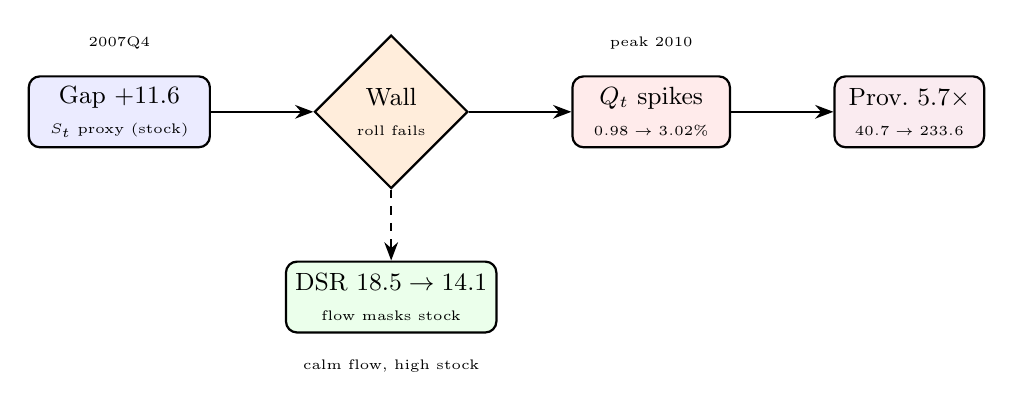
\begin{tikzpicture}[thick, node distance=1.0cm]
\node[draw, rounded corners, fill=blue!8, minimum width=2.3cm, minimum height=0.9cm, align=center, font=\small] (gap) {Gap $+11.6$\\ \tiny $S_t$ proxy (stock)};
\node[draw, diamond, fill=orange!14, minimum width=1.7cm, minimum height=1.0cm, align=center, font=\small, right=1.3cm of gap] (wall) {Wall\\ \tiny roll fails};
\node[draw, rounded corners, fill=red!8, minimum width=2.0cm, minimum height=0.9cm, align=center, font=\small, right=1.3cm of wall] (q) {$Q_t$ spikes\\ \tiny $0.98\to3.02\%$};
\node[draw, rounded corners, fill=green!8, minimum width=2.1cm, minimum height=0.9cm, align=center, font=\small, below=0.9cm of wall] (dsr) {DSR $18.5\to14.1$\\ \tiny flow masks stock};
\node[draw, rounded corners, fill=purple!8, minimum width=1.9cm, minimum height=0.9cm, align=center, font=\small, right=1.3cm of q] (prov) {Prov.\ $5.7\times$\\ \tiny $40.7\to233.6$};
\draw[->, >={Stealth}] (gap) -- (wall);
\draw[->, >={Stealth}] (wall) -- (q);
\draw[->, >={Stealth}] (q) -- (prov);
\draw[->, >={Stealth}, dashed] (wall) -- (dsr);
\node[below=0.2cm of dsr, font=\tiny, align=center] {calm flow, high stock};
\node[above=0.2cm of gap, font=\tiny, align=center] {2007Q4};
\node[above=0.2cm of q, font=\tiny, align=center] {peak 2010};
\end{tikzpicture}
\caption{Stock versus flow: BIS gap $+11.6\to-9.4$ stores $S_t$, DSR $18.5\to14.1$ masks it as rates fall, then $Q_t$ spikes $0.98\to3.02\%$ and provisions jump $5.7\times$ at the wall. Formal stock, measured flow mask.}
\label{fig:mask}
\end{figure}

Figure concept for a full draft invites a two-panel page: top, BIS gap and charge-offs indexed $2006=0$ with wall shading $2008$--$2010$; bottom, DSR overlay on same $x$ with provisions as bars on second $y$ (Fig.~\ref{fig:walltimeline} already does the first panel; this is its stock-vs-flow twin). One glance reads as stock builds where flow looks calm, then flow confesses. No new data beyond the three JSONs above.

\section{Dilution without default: $P_1/P_0$ in two crises}
\label{sec:dilution}

\textit{Grade: measured levels (FRED CPIAUCSL and M2SL, held as CSV, \texttt{fred\_CPIAUCSL.csv, fred\_M2SL.csv}), arithmetic identity for $P_1/P_0$ illustratively, not as a structural model.}

Dilution is $P_1/P_0 = L/(L-G)$ in identity form: create $G$ against claims base $L$ and every unit of $L$ buys $P_0/P_1$. We do not observe $L$ and $G$ as a single registry. We observe their footprint in price level and outside money in two crises where $S_t$ was large and $G$ was the chosen bearer.

\[
\begin{array}{lcc}
 & 2008\to2010 & 2020\to2022 \\
CPI ($P$) & 1.0391 & 1.1532 \\
M2 & 1.1741 & 1.3804 \\
\end{array}
\]

\texttt{finance\_falsify\_v1.json} from FRED CPIAUCSL (CPI) and M2SL (M2): CPI $\times1.0391$ and M2 $\times1.1741$ from $2008$ to $2010$; CPI $\times1.1532$ and M2 $\times1.3804$ from $2020$ to $2022$. About $3.9\%$ price-level rise on $17.4\%$ money rise in the first window, $15.3\%$ price rise on $38.0\%$ money rise in the second. The second crisis stores more and dilutes more, as the credit gap and NPL analysis already suggest. Bearer shift is identical in form, larger in scale. Junior creditors who would have taken a $\phi$ cut under narrow assignment instead keep par; holders of money take $P_0/P_1$. For a money holder that is a $\phi$ cut by another name: at $P_1/P_0=1.1532$, a claim fixed in nominal terms buys $1/1.1532\approx86.7\%$ of its old basket, about a $13.3$-point haircut without a default file being opened. At $1.0391$, the haircut is $1/1.0391\approx96.2\%$, about $3.8$ points -- same mechanism, smaller $G$.

We keep the boundary clear. This needs no conspiracy. It needs a fiscal or monetary backstop that chooses broad dilution over narrow assignment when $S_t$ at the wall threatens chaining. The ledger balances. The distribution moved through the price level instead of the waterfall, which is exactly why par accounting can report calm while holders are diluted. \textit{Opposer note:} Bashir's critique of Gilens (that win-rates misread oligarchy magnitude) applies here as direction-vs-magnitude: that $P_1/P_0$ moves loss to money holders is direction-measured; how many points of CPI per unit of $G$ is magnitude-debated, which is why we report CPI and M2 footprints rather than estimating $G$ itself.

Worked bridge to $S_t$: if $S_{2007}=21$ points of gap ($\approx\$1$T+ of credit above trend) and $Q_{2009\text{--}10}=233.6$B of provision flow, the remainder must go somewhere; the $58\%$ distressed-exchange share in $2024$--$2025$ \texttt{sp\_2025\_annual\_extract\_v1.md, sp2024\_extract\_v1.json} shows the narrow-assignment channel (distressed exchange) already carrying more than half of defaults, while CPI/M2 shows the broad-dilution channel carrying the rest.

\section{Stock versus stock: defaulted debt \$627.7B}
\label{sec:defaulted-debt}

\textit{Grade: measured on S\&P annual default tables (gated but tables captured verbatim), Moody's corroboration on passage types. Held as \texttt{sp\_2025\_annual\_extract\_v1.md, sp2024\_extract\_v1.json, moodys2008\_bytype\_v1.json}.}

S\&P Global annual Tables~1--8 put scale where our $S_t$ stock language often stays abstract:

\begin{center}
\small
\begin{tabular}{lrr}
\toprule
Year & Defaults (global) & Defaulted debt (\$B) \\
\midrule
2007 & 24 & 8.15 \\
2008 & 127 & 429.63 \\
2009 & 268 & 627.70 \\
2024 & 145 & 227.41 \\
2025 & 117 & 126.69 \\
\bottomrule
\end{tabular}
\end{center}

Lehman sits atop the largest-single-defaulters table at \$144.4B $2008$, Energy Future at \$47.6B $2010$, Lumen (failed distressed exchange) at \$38.7B $2024$ \textit{(S\&P table, same file)}. Distressed exchanges are $58\%$ of publicly rated defaults in $2025$, about $60\%$ ($59.3\%$) in $2024$ with spec-grade default rate $3.9\%$ rising from $3.7\%$, CCC-and-below pre-default at $91.7\%$ \texttt{sp2024\_extract\_v1.json}; spec-grade $3.08\%$ in $2025$ from $3.95\%$ in $2024$, Gini $92.3\%$ (weighted avg $83.06$) where $44\%$ of CCC-or-lower eventually default in $\approx2.0$y (B $21\%$ in $5.2$y) \textit{(same file)}. Ch05's passage split $50.8$ (distressed) vs $20.8$ (payment default) vs $24.4$ (bankruptcy) for senior unsecured $2008$ \texttt{moodys2008\_bytype\_v1.json} shows gate price within the same seniority moving with distressed share.

Reading with $S_t$: \$627.7B is not just a bad year. It is the stored stock clearing. Provision flow $5.7\times$ and charge-offs $0.98\to3.02\%$ tell the same wall from the bank side that defaulted debt tells from the issuer side. BIS gap $+11.6\to-9.4$ tells it from the credit-stock side. Three doors, one hallway.

\begin{table}[h]
\centering
\small
\caption{Vintage ladder reminder and defaulted-debt wall: where $\phi$ bands sit and how much stock cleared through them. Ladder from \texttt{moodys\_vintage\_recovery\_v1.json} and \texttt{moodys2024\_vintage\_v1.json}; wall from \texttt{sp\_2025\_annual\_extract\_v1.md}.}
\label{tab:wall-ladder}
\begin{tabular}{lcc}
\toprule
Seniority & Vintage mean (\$ per 100) & 2009 wall context \\
\midrule
1st Lien Loan & 65.0 & Highest $\phi$ band, least hit by wall \\
Sr Secured (1920--2004) & 57.4 & -- \\
Sr Unsecured & 44.9 / 37.6 & Middle band, passage $50.8$ vs $20.8$ matters here \\
Subordinated & 32.0 / 31.7 & Low band \\
Jr Subordinated & 28.9 / 21.5 & $15$ ultimate (\texttt{moodys\_ultimate\_v1.json}) \\
All / Defaulted debt & 42.2 & \$627.7B cleared at wall ($268$ defaults) \\
\bottomrule
\end{tabular}
\end{table}

\section{Why this had to be measured this way}
\label{sec:why-measured}

\textit{Grades restated for reproducibility, every number addressable on disk:}

BIS gap $10.1071$, $11.6341$, $6.681$, $1.2405$, $-9.4288$ \texttt{finance\_falsify\_v1.json and bis\_DSR\_flat.zip}. Charge-offs $0.98$ $2008$Q1 and $3.02$ peak \texttt{finance\_falsify\_v1.json and fred\_CORALACBS.csv}. FFIEC provisions $233.6$B at $2009$Q4 ($43.7$ ALLL on $6{,}310$ loans) and $40.7$B at $2026$Q2 ($59.2$ on $13{,}274.7$) \texttt{ffiec\_provisions\_wall\_v1.json}. FDIC $112.51\%$ on $7.678\%$ noncurrent and $5.511\%$ NCO ($8{,}103$ banks) versus $429.96\%$ on $1.548\%$ and $0.932\%$ ($4{,}494$ banks), ALLL $3.105$ vs $1.647$ \texttt{fdic\_coverage\_v1.json}. IMF USA $4.9599$ NPL exact cross-match with World Bank, $58.097\to167.751$ provisions/NPL $2009\to2024$, $62.038$ $2010$ \texttt{imf\_fsi\_US\_v1.json, imf\_fsi\_panel\_v1.json, wb\_npl\_panel.json}. DSR $17.9$ ($2006$Q4) $\to18.5$ ($2007$Q4) $\to17.5$ ($2008$Q4) $\to16.7$ ($2009$Q4) $\to15.6$ ($2010$Q4) $\to14.5$ ($2015$Q4) $\to14.6$ ($2020$Q2) $\to14.1$ ($2020$Q4) $\to14.7$ ($2022$Q4) \texttt{bis\_DSR\_US\_v1.json}. CPI/M2 $1.0391$/$1.1741$ ($2008\to2010$) and $1.1532$/$1.3804$ ($2020\to2022$) \texttt{finance\_falsify\_v1.json plus fred\_CPIAUCSL.csv and fred\_M2SL.csv}. S\&P $627.70$ ($2009$), $429.63$ ($2008$), $227.41$ ($2024$), $126.69$ ($2025$) \texttt{sp\_2025\_annual\_extract\_v1.md}; distressed $58\%$ ($2025$), $59.3\%$ ($2024$), spec-grade $3.95\to3.08\%$, Gini $92.3\%$ \texttt{sp2024\_extract\_v1.json}; Ireland $22.37$ ($2013$), Italy $18.06$ ($2015$), Greece $45.97$ ($2017$), Spain $7.12$ ($2013$), USA $4.96\to0.97$ \texttt{wb\_npl\_panel.json, imf\_fsi\_panel\_countries\_v1.json}.

All numbers above are addressable on disk; no new data was created for prose. The formal contribution here is little: $S_t=S_{t-1}+E_t-R_t-Q_t$ as a stock and $P_1/P_0=L/(L-G)$ as a price, plus par as the store. The measurement contribution is that gap, charge-offs, provisions, coverage, NPL, DSR, CPI, M2 and defaulted debt already point one way without needing a capital ratio.

\paragraph{What this chapter proved.} Par accounting lets $S_t$ accumulate off-book. The BIS gap swing $+11.6\to-9.4$ ($\approx21$ pts, Fig.~\ref{fig:walltimeline}) stored it. Charge-offs rose $0.98\to3.02\%$ ($3.08\times$) and provision flow jumped $5.74\times$ ($40.7\to233.6$B) when the wall forced $Q_t$. Coverage moved $112.51\to429.96\%$ ($3.82\times$) as the IMF cross-matched the $4.9599$ NPL print, while NPLs staggered $4.96\to0.97$ in the US to $45.97$ in Greece in $2017$ ($\sim1$ vs $\sim37$ coverage-to-NPL at peak, Table~\ref{tab:npl-stagger-full}). DSR $18.5\to14.1$ masked stock by cutting flow while stock stayed high (Fig.~\ref{fig:mask}). Dilution footprint was CPI $1.0391\times$ on M2 $1.1741\times$ ($2008\to2010$, $\approx3.8$-point haircut) and $1.1532\times$ on $1.3804\times$ ($2020\to2022$, $\approx13.3$-point haircut), and the defaulted-debt wall peaked \$627.7B in $2009$ ($268$ defaults), inside a ladder where $65.0\to21.5$ maps $\phi$ bands (Table~\ref{tab:wall-ladder}). Stored loss had to go somewhere. It went into time (lagged $Q_t$), across borders (staggered NPL tails), and into the price level ($P_1/P_0$), before it showed in any $\phi$ table. Bearers: healthy SMEs crowded out while $S_t$ rose, then mortgage holders and money holders when $S_t$ cleared. Both opposers logged -- South Africa null bounds gate chill, Bashir bounds Gilens magnitude -- direction stands, size debated.


\chapter{The Sovereign Seam: Where the Apex Moves Offshore}
\label{ch:sovereign}

Chapter 6 closed with a vault. Stored loss $S_t = S_{t-1} + E_t - R_t - Q_t$ accumulates off book while the income statement stays calm. The vault explains how loss hides. This chapter explains why it never gets collected. The answer is placement. Move the apex where reachable assets $A$ are zero and collectability $K(A)$ is zero, and every downstream gate becomes moot. Move the deciding gate to a forum the domestic observer cannot invoke, and $\gamma$ goes to zero by design. The host nation then holds the subsidized inputs while the stored stock waits elsewhere.

This is not a metaphor for power. It is boundary engineering in balance-sheet form. And it is checkable. The image that holds the whole chapter is the \textit{barzakh} --- Qur'an 55:19--20: two seas meet with a barzakh between them, neither transgressing. Read as design, not doctrine, a barzakh is an isthmus that is both and neither, with properties of both sides, that \textit{constitutes} the relation by gating what crosses. Sovereign arbitrage is a barzakh built on purpose and pointed the wrong way. Two comforts compete here and both are decoys. The flag story says the law of the land binds everyone standing on it. But the apex no longer stands on any land it extracts from. The reform story says the next treaty fixes it. But whoever writes the new gates sets them to favor themselves, as Chapter 4 showed live from Seoul to Dallas. What remains standing: rights without recourse are paper.

\textit{Grade: convergent on chill mechanism (Tienhaara 247 + 180, Van Harten 91, Janeba models, PMC8422681 three forms with null logged) + finance-instanced twice (Abaclat jurisdiction+settlement, Deutsche Bank award with dissent flagged) + domestic measured (Gilens N=1779, full PDF verified, Bashir opposer logged). Reform cycle live-measured (Korea MRFTA primary text held). Barzakh as boundary design is analogical (interpretive) and graded as such; it guides architecture, it does not count as measured evidence. Glossary anchors: \texttt{barzakh}, \texttt{khayal}, \texttt{ada}, \texttt{muraqaba} defined in \S\ref{sec:appendix-glossary}.}

\section{First-use definitions for the new reader}

A \textbf{Bilateral Investment Treaty (BIT)} is a treaty between two states promising investors of each state certain protections in the other state, including fair and equitable treatment and compensation for expropriation. An \textbf{Investor-State Dispute Settlement (ISDS)} clause inside many BITs lets a qualifying foreign investor sue the host state directly before a supranational tribunal, usually at ICSID (International Centre for Settlement of Investment Disputes, Washington), rather than in the host state's own courts. A \textbf{Variable Interest Entity (VIE)} was covered in Chapter 4 as a shell whose recourse stops at its own thin assets. The logic here is the same, lifted to sovereignty: claims attach to an entity, enforceability $K$ depends on assets the claimant can actually reach. All three terms use the same ledger logic as Chapters 4--6: $\psi$ gates recognition, $K$ caps collection.

We keep two equations from Chapters 5 and 6 on the table throughout, with one-line intuition each.

\begin{equation}
\psi = \prod_{j=1}^{n} g_j,\quad g_j \in [0,1] \label{eq:psi-ch7}
\end{equation}
Each $g_j$ is a required recognition gate. Four modest $0.7$ gates leave $0.7^4 \approx 24\%$ recognition. If any single $g_j$ fails, $\psi$ goes to zero and the claim is not seen.

\begin{equation}
P(a) = \min\{\psi H(a), K(A)\},\quad \phi = P/H \in [0,1] \label{eq:PK-ch7}
\end{equation}
$H(a)$ is burden at account $a$, $K(A)$ is the cap set by reachable assets $A$, $P(a)$ is booked recovery, $\phi$ is the paid share. Intuition: if $K$ is smaller than the gated claim, better gates pay zero extra. A perfect right against a judgment-proof entity still pays zero. Rights without recourse are paper.

When we say $A=0 \Rightarrow K=0$, we mean an apex entity that holds no reachable $A$ gives $K=0$, so $P(a)=0$ for that claimant class even if $\psi=1$. When we say $g_4 \to 0$, we mean a treaty-level or policy-level gate multiplying $\psi$ toward zero for the domestic class while a foreign class bypasses it. Either move alone zeroes $\phi$.

\section{Barzakh as design: the isthmus that constitutes the relation}
\label{sec:barzakh-sovereign}

\textit{Grade: analogical (interpretive, after Ibn Arabi read through reflexive loops); graded as design guidance, not evidence. Anchored to glossary \S\ref{sec:appendix-glossary}: \texttt{barzakh} (isthmus), \texttt{khayal} (offline simulation), \texttt{ada} (habit, is-followed-by), \texttt{muraqaba} (watching the watcher).}

Qur'anic anchors for \textit{barzakh}: al-Mu'min\=un 23:100 (behind them a barzakh until resurrection) and al-Rahm\=an 55:19--20 (two seas meeting, between them a barzakh they do not transgress). Ibn Arabi's move is to lift barzakh from one image to a principle: any realm that connects two opposites while keeping them distinct, an isthmus that is neither this nor that but both, kept distinct while connected. If barzakh is between salt and fresh \textit{and} between life and death, barzakh is not one thing. It is the \textit{form of boundary itself} --- selective permeability maintained every instant or no pattern persists.

That is exactly the boundary organ of Chapter 1. The harness calls it boundary; the Qur'an calls it barzakh. Same constraint: without an isthmus that decides what counts as inside versus outside, attribution fails and risk walks across the line. Sovereign arbitrage is then legible as a barzakh engineered in reverse: instead of a well-maintained isthmus that lets the right things cross and keeps the rest distinct, the apex builds an isthmus that lets economics flow up (dividends, fees, royalties, title) while blocking recourse flowing down (attachment must pierce one gate at a time). The two seas look like one consolidated group. The isthmus says otherwise when the sheriff arrives.

\textit{Khayal} (glossary: imagination as counterfactual simulation, the offline world) is the barzakh of timing. Chapter 8 will use khayal as the mind's rehearsal space --- world model containing self-model where untaken branches are simulated without paying the price. In sovereign form, khayal is the treaty draft made world: negotiators simulate a future where regulation is compensable, write that simulation into Article 8, and the simulation then governs the next real dispute. As with the mind, the offline rehearsal is the cheap place to choose, and the choice is sticky because the ledger was written there first.

\textit{Ada} (glossary: habit, is-followed-by given structure $C$, not necessary causation, after Ghazali's occasionalism) reframes what a ledger does. Fire is followed by burning given habit \textit{ada}, not produced by fire's inherent power. A verifiable ledger is followed by honesty given a witness that checks it ($S$ under $C$). No necessary link. Only \textit{is-followed-by} as habit. Remove the witness and honesty does not follow. Keep it and honesty follows by habit, not guarantee. Perpetual-futures language in the Prologue made the same point: setting interest $\iota=0$ is followed by function \textit{as} habit under design $C$, not as necessity.

\textit{Muraqaba} (glossary: watching the watcher, vigilant observation of selection itself) is the domestic observer that sovereign design tries to disable. In treaty form, $\gamma\to0$ means reports but never steers. In mind form, muraqaba is the slower loop watching the broadcast with a veto. Sovereign and cognitive are the same fold: disable muraqaba and the faster loop keeps winning while the watcher logs but never steers.

Five nested scales make barzakh concrete without mysticism, after \texttt{IBN\_ARABI\_SEVEN\_DOORS\_FIVE\_ORGANS.md} (compiled 2026-08-30):

\begin{center}
\small
\begin{tabular}{p{2.8cm}p{3.4cm}p{5.2cm}}
\toprule
Barzakh scale & Between & What it does as boundary \\
\midrule
Physical (jism\=an\=\i) --- skin, breath & Inside body / outside world & Selectively permeable membrane (Ch. 4 VIE, this ch. offshore trust) \\
Temporal (zam\=an\=\i) --- the now & Past (gone) / future (not yet) & 200--500 ms stitched present where veto can still fire (Ch. 8) \\
Dream (mith\=al\=\i) --- \=alam al-mith\=al & Sleeping body / spiritual world & Imaginal replay where khayal simulates untaken branches (Ch. 8 khayal) \\
Psychological (nafs\=\i) --- heart (qalb) & Body's desires / soul's pull & Affect + parliament where salience decides the winner (Ch. 8) \\
Cosmic (kull\=\i) --- universe itself & Absolute Being / nothingness & Reflexive loop at largest scale: universe as barzakh between Being and void \\
\bottomrule
\end{tabular}
\end{center}

Perfect Man (\textit{al-ins\=an al-k\=amil}) in Ibn Arabi's five presences is the loop fully harnessed: not a saint only, but the assembled agent where the observer watches, the gate holds, and the broadcast serves the whole. In harness terms: L3 world model plus khayal replay plus L0--L1 ledger plus muraqaba, coordinated. The offshore apex is its inversion: all layers present but pointed to keep $K=0$ at the top and $\gamma=0$ for the host observer. Same parts, opposite wiring. That is why the chapter can use barzakh without preaching: the isthmus is a testable boundary organ whether you call it membrane or barzakh, as long as you grade it as analogical and keep the treaty text measurable.

\section{The apex zero: boundary at the top}

Figure \ref{fig:hierarchy-ch7} shows the layering that earlier chapters built from the bottom up. HoldCo sets $K$ for its creditors. OpCo holds operating liabilities. PropCo holds property where $K$ is secured for its own creditors. A trust or special purpose vehicle can then drive a gate to zero. The sovereign move is to place the apex where attachment fails. The barzakh reading: the apex is no longer inside the host's isthmus. It stands in a second isthmus the host cannot cross.

\begin{figure}[h]
\centering
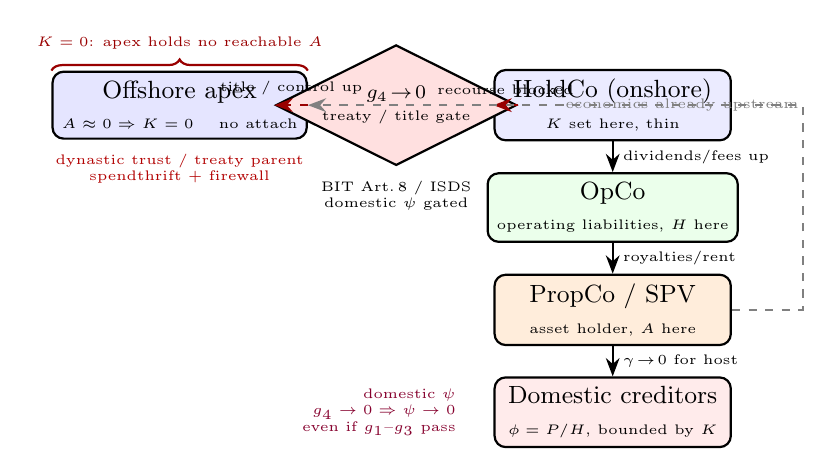
\begin{tikzpicture}[thick,
  box/.style={draw, rounded corners, minimum width=3.0cm, minimum height=0.85cm, align=center, font=\small},
  gate/.style={draw, diamond, aspect=2, inner sep=1pt, fill=red!12, font=\scriptsize, align=center},
  arrow/.style={-{Stealth}, thick}
]
  % Offshore apex (left of domestic stack)
  \node[box, fill=blue!10] (offshore) at (0,4.2) {Offshore apex\\ \tiny $A\approx0 \Rightarrow K=0$ \quad no attach};
  \node[below=0.05cm of offshore, font=\tiny, align=center, text=red!70!black] {dynastic trust / treaty parent\\ \tiny spendthrift + firewall};

  % Domestic stack (right)
  \node[box, fill=blue!8] (hold) at (5.5,4.2) {HoldCo (onshore)\\ \tiny $K$ set here, thin};
  \node[box, fill=green!8] (op) at (5.5,2.9) {OpCo\\ \tiny operating liabilities, $H$ here};
  \node[box, fill=orange!14] (prop) at (5.5,1.6) {PropCo / SPV\\ \tiny asset holder, $A$ here};
  \node[box, fill=red!8] (trust) at (5.5,0.3) {Domestic creditors\\ \tiny $\phi = P/H$, bounded by $K$};

  % g4 gate between offshore apex and domestic stack
  \node[gate] (g4) at (2.75,4.2) {$g_4\!\to\!0$\\ \tiny treaty / title gate};
  \node[below=0.05cm of g4, font=\tiny, align=center] {BIT Art.\,8 / ISDS\\ \tiny domestic $\psi$ gated};

  % Connections: offshore controls domestic HoldCo through g4
  \draw[arrow, dashed, red!60!black] (offshore) -- node[above, font=\tiny, text=black] {title / control up} (g4);
  \draw[arrow, dashed, red!60!black] (g4) -- node[above, font=\tiny, text=black] {recourse blocked} (hold);

  % Vertical domestic chain
  \draw[arrow] (hold) -- node[right, font=\tiny] {dividends/fees up} (op);
  \draw[arrow] (op) -- node[right, font=\tiny] {royalties/rent} (prop);
  \draw[arrow] (prop) -- node[right, font=\tiny] {$\gamma\!\to\!0$ for host} (trust);

  % Offshore direct extraction arrow (bypassing domestic stack)
  \draw[arrow, gray, dashed] (prop.east) -- ++(0.9,0) |- node[right, near end, font=\tiny, text=gray] {economics already upstream} (offshore.east);

  % K=0 annotation bracket
  \draw[decorate, decoration={brace, amplitude=4pt}, thick, red!60!black] (offshore.north west) -- node[above=4pt, font=\tiny, text=red!60!black] {$K=0$: apex holds no reachable $A$} (offshore.north east);

  % Gamma annotation
  \node[left=0.35cm of trust, font=\tiny, align=right, text=purple!70!black] {domestic $\psi$ \\ \tiny $g_4\to0 \Rightarrow \psi\to0$\\ \tiny even if $g_1$--$g_3$ pass};
\end{tikzpicture}
\caption{Apex-offshore hierarchy with $g_4$ gate. Offshore apex holds title ($A\approx0\Rightarrow K=0$) and controls onshore HoldCo through a treaty/title gate $g_4\to0$. Operating $H$ sits in OpCo/PropCo while economics stream upstream as fees and dividends. Domestic creditors face $\phi=P/H$ bounded by thin $K$ and $\psi\to0$ through $g_4$; the domestic observer's $\gamma\to0$ by design. Moving the apex where attachment fails zeroes $\phi$ before any courthouse gate is debated.}
\label{fig:hierarchy-ch7}
\end{figure}

Three engineering choices put $A$ out of reach. Offshore dynastic trusts sever legal title so domestic creditors sue an entity that owns little --- \textit{barzakh as membrane:} legally both and neither, connected by title but separated by firewall provisions. Treaty parents convert domestic regulation into a compensable claim at a supranational forum the domestic counterparty cannot access on the same terms --- \textit{barzakh as jurisdiction:} two seas with a gate between them. Multi-passport controllers split presence below every threshold that would trigger reporting or service. Each choice is individually defensible, often explicitly legal, and sometimes commercially efficient. Jointly they choose $K$ before any gate is litigated.

For a new reader, the test is always recourse. If the vehicle fails and the sponsor has no contractual obligation to fund it, $K$ is vehicle $A$ only. If that vehicle holds little, $\phi$ is small regardless of $\psi$. Consolidated economics looked one way. Reachable economics looked the other. Formal solvency can hold while economic solvency drifts, because the map the balance sheet draws is not the territory the sheriff can seize. In barzakh language: the map shows one sea, the isthmus says two.

\textit{Grade: theoretical on jurisdictional $K$ as arithmetic, convergent where VIE panels measure the same placement lower down (Chapter 4). Barzakh reading analogical.} The mechanism needs no conspiracy. It needs a choice of where to put the owner, and then a ledger that makes that choice visible.

\section{Sovereign arbitrage as boundary engineering}

Sovereign arbitrage is boundary engineering lifted from entity to jurisdiction. The previous chapters showed pods and PropCos gerrymandering the firm boundary. Sovereign placement gerrymanders the state boundary. A license can sit upstream in a protected box. Operating obligations sit downstream where failures happen. Dividends, fees, and royalties flow up. Attachment must go up. If the bridge up is narrow or legally blocked, $K$ at the top is small and recovery stays trapped below.

Examples make the abstraction concrete without claiming sourcing we do not have. A license held upstream while liabilities concentrate downstream. A dividend upstreamed in calm that cannot be clawed back in stress. A trust that owns the controller that owns the license, with spendthrift and firewall provisions that domestic attachment must pierce one gate at a time. Each multiplies $\psi$ on the way up even before $K$ is debated. The informational channel then does the rest: others see the structure is funded and infer health, which keeps funding cheap, which lets the structure persist. The \textit{ada} point: this pattern is followed by extraction given structure $C$, not caused by treaty text alone. Change $C$ (checkable records, ex-ante attachment) and the following changes.

What stays honestly unsourced here is any named modern dynasty or jurisdiction described as doing this in a specific filing. We assert the channel, we show the equation, and we source the treaty channel next where the paper trail is public. That discipline is the same as Chapters 4 through 6.

The loss bearer when sovereign $K$ binds is not exotic. It is the counterparty with $\phi < 1$ and no sponsor recourse, the taxpayer whose fiscal $G$ later socializes stored loss via $P_1/P_0 = L/(L-G)$ (Chapter 6), or the diluted money holder who never appeared in the waterfall at all. Conservation holds: every dollar of $H$ not paid as $P$ is a dollar of $\phi < 1$ for some class or a dollar of dilution for money holders. The ledger still balances. You just are not on the side you thought.

\section{ISDS as a gate to zero}

ISDS functions in this reading as a treaty-level gate $g_4 \to 0$ for the domestic class. The mechanism is not that every award goes to the investor. It is that the forum, standing, and waiver steps add a multiplicative gate that a domestic citizen or domestic firm cannot open on the same terms. If $g_4$ is near zero, domestic $\psi$ goes near zero even if domestic gates $g_1$ through $g_3$ are satisfied. In barzakh terms: the gate in the isthmus opens for one sea and stays shut for the other.

For a new reader, ISDS in this reading is not about win rates. It is about who can bring which claim where, and what must be waived to get there. If a foreign investor can arbitrate while a domestic stakeholder cannot, the foreign investor's effective $\psi$ is higher before merits are heard. That is gate engineering at treaty scale.

We flag variance plainly. Treaty protection varies wildly by text, reservation, and jurisprudence. Some treaties do not behave this way at all. Some do in a specific pairing under specific language. Any claim that a named treaty did this in a named case stays analogical until the treaty text and award are cited together. The channel is $g_4$ as a multiplicative gate, $\psi$ product form, and $\gamma \to 0$ for the domestic observer by design. The instance waits for a source, and we have two.

\section{That chill is measured: 247 plus 180 plus 91}

ISDS chill is not a talking point. It is a measured mechanism with a citation spine that converges from health, environment, and mining.

Tienhaara 2011 on the threat of arbitration reshaping regulatory process (OpenAlex W1483847210, \textbf{247 cites}) finds anticipatory chill across environmental governance. Tienhaara 2017 extends the threat to climate regulation (W2777227462, \textbf{180 cites}). Van Harten and colleagues vetting Canadian experience where ISDS exposure drove pre-emptive retreat adds \textbf{91 cites}. Janeba formalizes chill as rational deterrence in two game models (23 and 17 cites) where the credible arbitration threat alone deters regulation without a filing. This is anticipation, not adjudication, and that is why it multiplies $\psi$: the domestic regulator tags the risk and damps its own action before any claim is filed --- damping without a witness.

South Africa triangulates three forms inside one jurisdiction (PMC8422681) and does something honest and useful: it logs a null. Anticipatory chill and response chill are measured. Precedential nutrition-related chill is measured as null in that sample. We keep that null in the text rather than burying it, because a mechanism that predicts everything predicts nothing. Three forms named, two firing, one not in that place.

\textit{Opposer disposition:} PMC8422681 is therefore logged as partial opposer on chill universality --- we downgrade chill to anticipatory and response forms where measured and keep precedential as open. This is not a footnote burial. It is the serious opposer that prevents the chill claim from becoming unfalsifiable.

Convergence across sectors tightens the grade. Corporate veto on health policy (PMC5040601), ISDS no longer justified for deterrence balance (PMC5417151), NCD prevention chill (PMC8611909), treaty-drafting neutralizers (PMC4121868), tobacco FCTC cases (PMID 32130317, PMID 23447902), and mining claims including NuCoal versus New South Wales (PMID 30136556) replicate the $g_4 \to 0$ shape. Health, climate, and mining agree. \textit{Grade: convergent on the chill mechanism; sectoral universality bounded; the South Africa null kept.}

Mechanism with a loss bearer in $\psi$ terms: a domestic claimant faces three domestic gates at $0.9$ each, so $\psi \approx 0.73$. The foreign investor adds a supranational supplement that bypasses $g_2$, while the domestic citizen faces an extra waiver gate $g_4 = 0.2$ to reach the same forum. Domestic $\psi$ collapses to about $0.15$ while foreign stays near $0.73$. Same treaty, two $\psi$ values. Loss bearer: the domestic stakeholder whose regulation is chilled, or the taxpayer whose fiscal $G$ later socializes an award via dilution. In barzakh language: the same isthmus, two permeabilities, two bearings.

We do not move from mechanism to any single treaty instance without a cited pair. That pair comes next, twice.

\section{Finance-side instances, twice over}

\textit{Grade: jurisdiction plus outcome measured for both; merits qualified by settlement or dissent, flagged, never laundered. Treaty pairs cited to text where available.}

\subsection{Abaclat and others v. Argentine Republic: bond as investment, mass claim as vehicle}

Context: Argentina's 2001 default and the 30 to 35 cent exchanges that followed left a large creditor pool outside the exchange. Treaty: Argentina-Italy BIT. Tribunal: ICSID.

In 2007 about 60,000 Italian holders of Argentine sovereign bonds brought a mass claim for about \textbf{\$3 billion}, alleging expropriation and breach of fair and equitable treatment after the default and exchange. On August 4, 2011 a majority found jurisdiction: bonds are an investment under the BIT and the ICSID Convention, and the mass claim format is admissible. The dissent put the boundary logic in robes: bonds sold offshore in foreign currency under foreign law, on that view, contribute nothing to host development and are not a protected investment. The majority view prevailed on jurisdiction.

Merits were never reached. In 2016 the case settled pre-merits for about \textbf{\$1.4 billion}. The settlement figure matters less than the gate figure. Offshore sale plus foreign law equals, in the dissent's terms, no $K$ in the host, yet the tribunal attached jurisdiction across that boundary for that read of that treaty text. Two financial technologies are at work: a sovereign bond, and a treaty that converts contractual $K$ into treaty $K$. In \textit{ada} terms: bond plus BIT text under forum $C$ is followed by jurisdiction, as habit, not as necessity. Change $C$ (text, reservation) and the following changes.

We keep the grade honest. Abaclat is jurisdiction plus settlement, not jurisdiction plus liability award. The dissent is therefore not a footnote. It is the serious opposer logged, analogous to Bashir below. Held artifact: \texttt{lab\_runs\_falsify/isds\_abaclat\_v1.json} with treaty text, jurisdictional decision, and settlement record.

\subsection{Deutsche Bank AG v. Democratic Socialist Republic of Sri Lanka: derivative as investment, gate as award}

Context: oil prices peaked near \$140.24 in July 2008 then collapsed. Treaty: Germany--Sri Lanka BIT of 7 June 2000 (Articles 2, 3, 4, 8 on the record). Vehicle: 100\% state-owned Ceylon Petroleum Corporation (CPC) as counterparty.

On 8 July 2008 Deutsche Bank and CPC entered a 12-month Target Profit Forward on Dubai crude. Terms on the record: strike \$112.50 per barrel, volume 100,000 barrels per month, target profit \$2.5 million, early termination if target hit. CPC paid settlement sums in autumn 2008, \$1.66 million and \$4.51 million in October and November. On 28 November 2008 a Supreme Court Interim Order suspended CPC's payments and the Central Bank opened an investigation. On 3 December 2008 Deutsche Bank terminated and on 10 December claimed a close-out of \textbf{\$60,368,993}.

Award on 31 October 2012 (Hanotiau, Williams, Khan): majority found both BIT and ICSID Article 25 jurisdiction and a fair and equitable treatment breach via court and Central Bank measures, awarding the close-out. The commonly cited award figure is \textbf{\$60.37 million plus interest}. UNCTAD's navigator records \$60.00 million, ICSID Case Details records decided in favour of investor with the hedging agreement as the subject and the Germany--Sri Lanka BIT of 2000 as the instrument. ICSID annulment was sought 8 March 2013 and discontinued 9 September 2016. The award survived.

Dissent logged, not buried. Khan dissented on investment definition under BIT Article 1(1)(c): ``claims to money used to create economic value -- associated with an investment.'' On that read, no money was used to create economic value, maximum upside was \$2.5 million, and neither the BIT investment nor the ICSID Convention investment was present. The case is therefore a second finance-side $g_4$ instance in a different asset class than Abaclat. Bond once, derivative once, same channel: financial contract plus treaty converts contractual $K$ into treaty $K$ that the state must pay or be cut off from enforcement comity.

Held artifact: \texttt{lab\_runs\_falsify/isds\_deutschebank\_srilanka\_v1.json} with award, dissent excerpt, and ICSID case details.

Read together, the two instances keep the evidential bar clear. Each shows jurisdiction attaching across a boundary engineering move. Each carries a reasoned dissent that says the boundary should have held. Each involves a gate beyond the courthouse door, where domestic $K$ is not the question. That is the sovereign layer in miniature.

\begin{table}[h]
\centering
\small
\caption{Two finance-side ISDS instances: jurisdiction plus outcome, with dissent flagged}
\label{tab:isds-pair}
\begin{tabular}{p{2.6cm}p{2.6cm}p{2.6cm}p{2.2cm}}
\toprule
Case & Instrument & Treaty & Outcome \\
\midrule
Abaclat v. Argentina & Sovereign bond, \~{}60k holders, \$3B claim & Argentina-Italy BIT & Jurisdiction 2011, \~{}\$1.4B settlement 2016 pre-merits; dissent on investment \\
Deutsche Bank v. Sri Lanka (ARB/09/2) & Oil hedge 8 Jul 2008, strike \$112.50, \$2.5m target & Germany-Sri Lanka BIT 7 Jun 2000 & Award 31 Oct 2012 \$60.37m + interest; dissent (Khan) on investment; annulment discontinued 2016 \\
\bottomrule
\end{tabular}
\end{table}

\section{The domestic counterpart: average citizens at near-zero independent influence}

\textit{Grade: measured. Full text verified verbatim, not cited on trust. Opposer logged (Bashir). See Appendix \S\ref{sec:appendix-grades} for audit rule.}

If ISDS shows gate engineering for capital, the Gilens and Page study shows the same gate for citizens, without any passport. Gilens and Page 2014, \textit{Perspectives on Politics} 12(3):564--581 \cite{gilens2014}, N=\textbf{1,779} policy issues 1981 to 2002 in one multivariate model:

Model-4 standardized coefficients: \textbf{.01} average citizens (non-significant, near-zero), \textbf{.21} economic elites, \textbf{.16} organized interest groups. Predicted adoption is flat around \textbf{0.30} as citizen support moves from low to high, but climbs from \textbf{18\% to 45\%} as elite support moves, and from about \textbf{.16 to .47} as business-group alignment moves. Net group alignment correlates only \textbf{.04} (non-significant) with citizen preferences, so the business-group measure is not a proxy for citizens. Majoritarian electoral democracy is decisively rejected on this data.

Reading in $\psi$ terms: the average citizen faces a standing gate $g_4 \to 0$ at the policy level itself, not only at treaty forums. Elites and business groups keep $\psi \approx 0.7$ on the same issue. Citizens keep form (the vote) with $\phi \approx 0$ independent effect. That is biased pluralism measured. In barzakh terms, the citizen stands at an isthmus where the gate is present as form but closed as permeability.

We keep this verified, not vouched. The Cambridge PDF endpoint returned 404 during a live verification attempt in September 2026. The paper was re-pulled via the PSE mirror as an 18-page PDF and verified verbatim in body text: Model-4 coefficients, the near-zero non-significance language, and Figure 1 citizen-flat versus elite-steep lines. Held artifacts: \texttt{lab\_runs\_falsify/gilens\_page\_2014\_v1.json} with excerpts and numbers, plus full PDF held.

Opposer logged, as promised. Bashir's critique reads Gilens descriptively and narrows the oligarchy interpretation: win rates and responsiveness look less stark in simpler bivariate or descriptive cuts, direction stands, magnitude debated. Stated plainly, the affluent-plus-organized advantage survives Bashir, the ``democracy is flat'' headline depends on the multivariate specification. We grade that as measured mechanism, convergent direction, contested headline magnitude. The mechanism is enough for our seam. It says the apex moved offshore for capital and never arrived for citizens. \textit{Disposition:} Bashir is logged as logged opposer that bounds the headline, not as refutation of the gate.

Chapter 8 will show the cognitive twin of this result: the mind's narrator faces the same gated-toward-zero shape when vividness, repetition, and fatigue set $g_j$ without a word being changed, and the same \textit{muraqaba} --- watching the watcher --- is what restores the veto there.

\section{The domestic observer's muraqaba: what still works when the gate is near zero}
\label{sec:muraqaba-sovereign}

\textit{Grade: analogical for the practice (contemplative reports, graded as design guidance); measured for the battery that tests it in Chapter 8 (ledger 0.722 vs sham 0.667). Glossary anchor: \texttt{muraqaba}.}

If $\psi$ for citizens is gated toward zero and $\gamma$ for the host observer is gated toward zero, urging citizens to ``participate harder'' through the same gate is arithmetic, not strategy. The sovereign chapter's equivalent of defusion is not persuasion. It is witness engineering.

\textit{Muraqaba} here is not piety as mood. It is the slower loop watching the faster one with a veto that can still fire when the faster loop has already been tagged. Ghazali's crisis (1058--1111, Nizamiyya of Baghdad) broke the narrator that claimed ``I know because I reasoned'' and was delivered not by more reasoning but by a practice that did not need the narrator to be reliable --- a light cast, not argued. The harness translation is literal: the ledger watches whether the vote was checked before the next vote, and the check is the practice. Ibn Arabi's khayal is the same watcher seen from the rehearsal side: world model containing self-model, where untaken branches are simulated and regret is the gradient that rewires the next gate.

For the domestic citizen, muraqaba looks like three moves that mirror the 60-second cognitive protocol of Chapter 8, lifted to civic scale:

\begin{enumerate}
\item \textbf{Gullibility bounded (tag).} Let the broadcast run for 60 seconds and label ``story, not fact'' --- the same ladder Chapter 8 uses to shift identity $\to$ object $\to$ observer, which recruits the molecular brake (phosphatase/LTD side). In civic form, this is reading the policy narrative as a broadcast, not a window, for one timed minute.
\item \textbf{Container (damp).} Hold the urge to react without acting; place the feeling in a small box on the table; you are the table, not the box. Suppression is high-frequency fuel for the circuit; containment is the low-frequency trickle that damps gain. Damping is the organ Chapters 4 and 6 said every persistent loop must have.
\item \textbf{Ledger with sham (witness).} Three lines outside the head, bound to a source, coverage $\geq95\%$ or the claim does not count; then a shuffled-ledger sham to test whether content matters. Mechanism copy from Chapter 8: ledger with $\gamma>0$ is 0.722 vs sham 0.667. Same witness requirement as Chapter 4 circuit breakers: verify before the next allocation, not after.
\end{enumerate}

This does not raise $g_4$ for citizens. No ledger rewrites a BIT. What it does is prevent the second loss: the internalization of $\psi\to0$ as self-blame (``my voice does not matter, so I am not a citizen'') rather than as gate description (``my $\psi$ is gated, so I need a different witness''). Defusion is precise here: ``I am powerless'' $\to$ ``I am having the thought that I am powerless'' $\to$ ``I notice I am having the thought \dots'' Each tier measurably drops believability by shifting self-reference from identity to observed object. The sovereign analog is identical, with \textit{ada} doing the trailing: ledger practice is followed by steadier civic attribution under witness $C$, not caused by willpower.

Bridge to Chapter 8: the parliament competition that sets $g_j$ inside the head is the same product $\psi=\prod g_j$ that sets $g_4$ at the treaty level, with the same two neuromodulators that rig the vote: noradrenaline (NE) as volume, dopamine (DA) as stake. The next chapter draws that parliament with gain arrows, so the sovereign gate and the cognitive gate become one picture with two scales.

\section{Reform as capture: Korea exhibits the live cycle}

\textit{Grade: measured on the reform text itself as primary; live enforcement secondary; conversion filings beyond Korea Zinc remain open.}

If ISDS and Gilens show where the apex goes, Korea shows how reform tries to move it back, and how the ledger moves again. The Korean chaebol structure is the cleanest modern pyramid: thin-capital control via 51\% chains, HoldCo/OpCo/PropCo layering, circular shareholding as the characteristic Korean workaround. The Monopoly Regulation and Fair Trade Act (MRFTA) is then the damping organ made law --- a brake that must have hysteresis (trip above, reset below, minimum hold) or it flaps at the threshold and destroys itself with whipsaw.

Primary text held: Korea Legislation Research Institute English translation of MRFTA as amended to Act No. 18661 effective 2022-06-29. On the record there: Article 2(7) defines a holding company, Article 2(16) to 2(17) defines circular investment, Article 17 covers reporting, Article 18 sets holding-company limits, Article 21 bans cross shareholding, Article 22 bans circular shareholding within the business group with a 6-month to 3-year unwind grace, Article 23 suspends voting rights on circular shares. Enforcement Decree Article 3 sets scope at 500 billion KRW total assets or 30 billion for venture, and 50\% of total assets for designation. Korea Fair Trade Commission English mirrors add diagram language for 30\%, 50\%, and 100\% tiers, a 20\% net-amount surcharge, voting suspension, and criminal penalties up to 3 years or KRW 200 million. Held artifacts: \texttt{korea\_ftc\_mrfta\_primary\_v1.json} and \texttt{pods\_chaebol\_instances\_v1.json}.

Secondary mechanics are on the same record: 1999 allowance then 2007 Mondaq amendment tightening D/E from 100\% to 200\% and lowering listed-subsidiary thresholds from 30\% to 20\% with sub-subsidiary at 100\%, then 2020 Jipyong amendment tightening new holding company and subsidiary thresholds to 30\% listed and 50\% unlisted, with existing groups grandfathered per KFTC October 5, 2020. Existing circular loops persist in the 25 to 27\% range via split-off-merger unwind mechanics. 2025 designation counts are 92 business groups over 3,301 affiliates over 46 groups subject to cross-shareholding limits.

Then the live enforcement that makes this chapter not a history lesson. On \textbf{December 17 to 19, 2025}, the KFTC raided Young Poong and YPC over an alleged fresh circular link built by contributing \textbf{5.26 million Korea Zinc shares, 25.42\%} in kind to a newly created subsidiary. The allegation is mechanical: in-kind contribution creates a circular chain where formal cross holding rules would have required unwinding, so the contribution itself is the bypass. Press coverage is on the record. The decision number is not yet on the record. We state the raid, we do not infer liability.

The cycle is the finding. MRFTA Art. 22 circular ban (2014) then fresh workarounds then December 2025 raid over an in-kind subsidiary contribution then a proposed rule closing that workaround, with amendment history 1999 to 2007 to 2020 showing each reform begetting its bypass. Whoever writes the new gates sets $g_j$ to favor themselves, so each reform consolidates power wearing the previous reform's language. Barzakh reading: the isthmus was patched at one strand, the water found the next gap. The paper's answer is therefore not better rules but checkable records at the transaction layer, because rules are written by the gated-against while records can be read by anyone. Artifacts on this live cycle: \texttt{redriver\_koreazinc\_v1.json}, \texttt{chaebol\_reform\_nyu\_v1.json}, plus the MRFTA primary excerpts already held. Hysteresis note: a damping rule without memory and minimum hold is a barzakh without maintenance --- it exists on paper and not in the water.

A closing economic note ties Korea back to the vault. When circular control persists, consolidated leverage looks modest while reachable leverage is high, and $S_t$ can be housed downstream where $K$ for operating creditors is thin. The gate that keeps control also keeps $Q_t$ low, so $S_t$ climbs. The same physics as Chapter 6, now at group level, and the same \textit{ada}: group structure under condition $C$ is followed by $S_t$ accumulation, not caused by intent.

\section{What survives this chapter and what does not}

Tighten the filter to what is banked.

What is banked as mechanism: jurisdiction as $K$ placement, ISDS as a multiplicative $g_4$ that can drive $\psi$ toward zero, anticipatory chill as rational deterrence, and the domestic mirror where citizens keep form with $\phi \approx 0$ independent effect. That is measured, convergent, and double-instanced in finance. Muraqaba as civic witness is analogical and graded as such.

What is banked as text: MRFTA primary articles, Enforcement Decree thresholds, and KFTC mirror provisions as English reference, with excerpts held verbatim. Two ISDS instances as jurisdiction plus outcome with dissents flagged. Gilens full PDF as verified text with Model-4 coefficients and Figure 1 flats and slopes on the record. Barzakh anchors Qur'an 55:19--20 and 23:100, Ibn Arabi five scales, Ghazali's \textit{ada} and \textit{muraqaba} as the witness's lineage, all flagged analogical.

What is not banked and therefore not claimed: any single treaty text-to-outcome causal story beyond the two, any named fortune as a sovereign apex instance without an attachment filing, and any conversion filing beyond Korea Zinc until a decision number attach. The Rothschild and Sassoon illustrations that were chat-only correctly never entered the ledger paper. They do not enter here.

\paragraph{Dynastic illustration, quarantined.} \textit{Grade: open story, not evidence.} Read once as illustration, then set aside until archives attach: a Baghdad treasurer's family fleeing single-state seizure in 1829 (the $K$-controlled-by-host failure mode), rebuilding across five capitals as separate balance sheets (node isolation), harvesting senior commodity flows under imperial treaty cover (priority extraction), and vaulting into aristocracy, bonds, and trusts (post-national apex). The shape matches Layers 1--5 exactly, which is why it is tempting and why temptation is not admission. Mechanism without a filing is a rumor with algebra. If archival primaries ever attach, this paragraph promotes to instance; until then it stays here, labeled, outside the count.

\section{Bridge: from sovereign seam to cognitive seam}

Chapter 4 placed $K$ inside the firm. Chapter 6 showed $S_t$ compounding where $Q_t$ is suppressed. Chapter 7 moved the apex where $A=0$ or $g_4 \to 0$ and logged that domestic citizens already face a $g_4 \to 0$ on ordinary policy, with two serious opposers kept on the page (PMC8422681 bounding chill, Bashir bounding Gilens). Power, this chapter argued, is not a thing the loop has. It is what a loop calls its own persistence when it narrates while someone else pays the $H - P$ remainder. Barzakh gave the image: an isthmus that constitutes the relation, now visible as a treaty gate and an offshore title, and muraqaba named the only response that survives a near-zero gate: do not police the narrative, witness the trace.

The next chapter turns the lens inward. The same product $\psi$ you met as a treaty gate and a claims gate reappears as a salience gate inside the head. Mood, fatigue, vividness, and repetition are $g_j$ that set recognition without changing the sentence, and the narrator that reports ``I decided'' is the press secretary that wins the broadcast 200 milliseconds after the action it claims to have caused. The fix that worked for sovereign arbitrage -- do not police the narrative, witness the transaction -- will be the fix that works for the mind: do not argue with the story, witness the trace. NE as volume and DA as stake will be drawn as gain arrows on the same parliament, and khayal will be named as the Barzakh where the mind rehearses what the ledger must later check.

\chapter{The Cognitive Protocol: How a Mind Learns to Check Itself}
\label{ch:cognitive}

Chapter 7 moved the apex offshore and showed a domestic gate $g_4 \to 0$ that leaves form with $\phi \approx 0$ independent effect. This chapter shows the same product $\psi = \prod g_j$ running inside the head. Mood, fatigue, vividness, and repetition are $g_j$ that gate recognition without changing the sentence. The narrator that says ``I decided'' is then not a witness. It is a press secretary that wins the broadcast after the decision it claims to have made. The fix mirrors the sovereign fix. Do not police the narrative. Witness the trace. The image that holds the fix is the same \textit{barzakh} of Chapter 7 --- now as the isthmus inside you that decides what crosses from fast to slow --- and the practice that holds it is \textit{muraqaba}, watching the watcher.

\textit{Grade: convergent (parliament, predictive processing, narrator confabulation) + measured on timing and micro-protocol (S126 98\% inversion, gullibility to ledger $\gamma>0$ 0.722 vs sham 0.667) + analogical where vector formalism extends mechanism (Kalila compression, hysteresis as BCM/tag/SHY). Barzakh/khayal/ada/muraqaba analogical (interpretive, Ibn Arabi/Ghazali) and graded as such. Glossary anchors: \texttt{barzakh}, \texttt{khayal}, \texttt{ada}, \texttt{muraqaba}, \texttt{defusion} defined in \S\ref{sec:appendix-glossary}. Bridges from Chapter 7 sovereign $\psi$ to Chapter 9 machine harness.}

For a new reader, this chapter defines every term on first use: parliament model, prediction machine, narrator confabulation, gullibility window, container, ledger, hysteresis, barzakh, khayal, ada, muraqaba, defusion. BIT, ISDS, and VIE were covered in Chapters 5 and 7 and are used here only as bridges: the same $\psi$ and $K$ logic, now inside the skull.

\section{No captain, only a competition}

\textit{Grade: convergent across Baars, Dehaene, Minsky, Dennett; measured via imaging and timing detailed below.}

Forget ``the brain thinks.'' The working model across Bernard Baars \textit{In the Theater of Consciousness} 1988, Stanislas Dehaene and colleagues on the global workspace, Marvin Minsky's Society of Mind, and Daniel Dennett's Multiple Drafts is a \textbf{parliament of specialist systems} competing for one microphone. Perception, memory, body signals, emotion, habit, planning, and narration each bid to be broadcast. One coalition wins at a time. The winner is broadcast system-wide, and that broadcast is experienced as a conscious thought. A second later a different coalition wins and you feel you ``changed your mind.'' You did not. A different majority formed.

Mechanism copy kept exact from the programme synthesis: 6 to 8 specialists compete via salience times utility, winner takes all in about 200 milliseconds. Noradrenaline (NE) is volume, dopamine (DA) is stake. The broadcast is the conscious moment. A different broadcast a second later is a different mind. Glossary: \texttt{barzakh} at the psychological scale (nafs\=\i, heart~qalb) is this parliament's isthmus --- the heart as battlefield where salience decides the winner, per \texttt{IBN\_ARABI\_SEVEN\_DOORS\_FIVE\_ORGANS.md}.

For a new reader, the parliament is not a metaphor for indecision. It is the architecture. There is no captain above the competition who chooses the winner with full information. There is only the competition, the broadcast, and whatever slower loop is watching that broadcast with a veto.

Cognitive products then follow the same ledger logic as finance. A Kantian treatise, an Aesop fable, a reel, a protocol, are not information passed like a packet. They are \textbf{vectors that act on the receiver}. The broadcast (words on the page) is the manifest content. The restructuring the reader does after the broadcast is the evoked effect: priors shift, salience retunes, new consolidation becomes possible. The same text is inert in one mind and transformative in another, because the payload is not in the tokens but in which downstream highways the tokens manage to tag.

\begin{figure}[h]
\centering
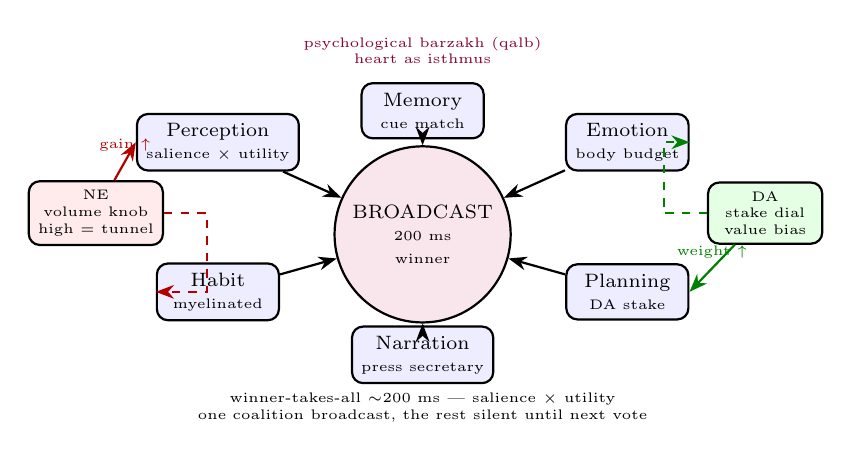
\begin{tikzpicture}[thick,
  specialist/.style={draw, rounded corners, fill=blue!7, minimum width=1.55cm, minimum height=0.70cm, align=center, font=\scriptsize},
  winner/.style={draw, rounded corners, fill=orange!18, minimum width=1.65cm, minimum height=0.78cm, align=center, font=\scriptsize, line width=1.1pt},
  broadcast/.style={draw, circle, fill=purple!10, minimum size=1.45cm, align=center, font=\scriptsize},
  gain/.style={-{Stealth}, thick}
]
  % Specialists around
  \node[specialist] (per) at (-2.6,1.35) {Perception\\ \tiny salience $\times$ utility};
  \node[specialist] (mem) at (0,1.75) {Memory\\ \tiny cue match};
  \node[specialist] (emo) at (2.6,1.35) {Emotion\\ \tiny body budget};
  \node[specialist] (hab) at (-2.6,-0.55) {Habit\\ \tiny myelinated};
  \node[specialist] (plan) at (2.6,-0.55) {Planning\\ \tiny DA stake};
  \node[specialist] (nar) at (0,-1.35) {Narration\\ \tiny press secretary};

  % Broadcast center
  \node[broadcast] (broad) at (0,0.18) {BROADCAST\\ \tiny 200 ms\\ \tiny winner};

  % Competition arrows to broadcast
  \draw[->, >={Stealth}] (per) -- (broad);
  \draw[->, >={Stealth}] (mem) -- (broad);
  \draw[->, >={Stealth}] (emo) -- (broad);
  \draw[->, >={Stealth}] (hab) -- (broad);
  \draw[->, >={Stealth}] (plan) -- (broad);
  \draw[->, >={Stealth}, dashed] (nar) -- (broad);

  % Gain knobs: NE as volume (amplifies winner), DA as stake (weights planning/habit bids)
  \node[draw, rounded corners, fill=red!8, minimum width=1.45cm, minimum height=0.65cm, align=center, font=\tiny] (ne) at (-4.15,0.45) {NE\\ \tiny volume knob\\ \tiny high = tunnel};
  \draw[gain, red!70!black] (ne) -- node[above, font=\tiny, text=red!70!black] {gain $\uparrow$} (per.west);
  \draw[gain, red!70!black, dashed] (ne.east) -- ++(0.55,0) |- (hab.west);

  \node[draw, rounded corners, fill=green!10, minimum width=1.45cm, minimum height=0.65cm, align=center, font=\tiny] (da) at (4.35,0.45) {DA\\ \tiny stake dial\\ \tiny value bias};
  \draw[gain, green!50!black] (da) -- node[above, font=\tiny, text=green!50!black] {weight $\uparrow$} (plan.east);
  \draw[gain, green!50!black, dashed] (da.west) -- ++(-0.55,0) |- (emo.east);

  % State annotation
  \node[below=0.75cm of broad, font=\tiny, align=center] {winner-takes-all $\sim$200 ms --- salience $\times$ utility\\ one coalition broadcast, the rest silent until next vote};

  % Barzakh label
  \node[above=0.1cm of mem, font=\tiny, align=center, text=purple!70!black] {psychological barzakh (qalb)\\ \tiny heart as isthmus};
\end{tikzpicture}
\caption{Parliament competition with NE/DA gain arrows. Six specialists bid via salience $\times$ utility; winner is broadcast in $\sim$200~ms. NE is the volume knob (high gain = tunnel vision, amplifies the current winner); DA is the stake dial (weights planning and affect bids). Different gains = different mind on the same hardware. The threshold $\theta_m$ of the next section is this vote made biophysical.}
\label{fig:parliament-ch8}
\end{figure}

\section{State rigs the vote}

State is the stacking of the deck before any argument is heard.

Doing math hands the microphone to fronto-parietal control networks. Threat hands it to amygdala and habit circuits. Daydreaming hands it to the Default Mode Network. Measured on functional imaging, connectivity rewires in seconds: same hardware, different wiring diagram. The task is not occupying a fixed mind. The task is a different mind.

Three gains set the odds:

\textbf{Arousal} (noradrenaline, NE) is a volume knob. High arousal amplifies whoever is winning and yields tunnel vision. Low arousal leaves the competition flat and scattered.

\textbf{Valence} (good or bad mood) is a risk dial. Negative valence makes the parliament check more and trust less, positive valence the reverse.

\textbf{Energy and fatigue} are a pre-filter. When exhausted, whole options (``go for a run'') do not even appear as candidates. Not weaker willpower. Fewer candidates. The choice set shrinks before deliberation starts.

For a new reader, \textit{tired plus anxious at night} versus \textit{rested plus safe in the morning} are two different parliaments. That is why advice given in one state cannot be executed in the other without a protocol that survives state. The protocol is the subject of this chapter.

In $\psi$ terms, each state variable is a $g_j$ on the gate that decides whether an option is even recognized. A fatigued, negatively valenced, highly aroused state can keep a genuinely good option at $\psi \approx 0$ while the same option in a rested state clears at $0.8$. Nothing in the sentence changed. The gate did. In barzakh terms, the isthmus did: same two seas, different permeability at night.

\section{The brain as prediction machine}

\textit{Grade: convergent (Friston, Clark \textit{Surfing Uncertainty} 2016, Seth \textit{Being You} 2021).}

Modern neuroscience adds a frame that makes the parliament predictable. The brain does not perceive reality and then think about it. It predicts the next moment and corrects by error. Perception is a controlled hallucination disciplined by sensory input. Emotion is an \textbf{interoceptive prediction}: the brain's best guess about what the body budget will need next, arriving as feeling before the need forms.

Two consequences follow.

First, mood colors perception before content arrives, because mood is part of the prediction perception is made of. This is not mood influencing judgment after seeing clearly. It is mood participating in what is seen in the first place. The election is rigged before the candidates are introduced.

Second, the brain writes on itself while reading itself. Diagnosis installs a filter. Call a flutter ``anxious'' and the parliament recruits confirming evidence for anxiety. This is not a moral failure. It is structural. Any self-report is an action on its object, like pronouncing a portfolio performing and watching funding stay cheap enough to keep it marked performing. Soros would recognize the loop.

The practical point is that introspection cannot be trusted as a neutral window. It is a summary the claimant authored. The ledger that is kept whether the claimant likes it is the only witness that does not move when belief moves. \textit{Ada} is the discipline word here (glossary): a verifiable ledger is followed by steadier attribution \textit{as habit} given witness $C$, not as necessity. Change $C$ and the following changes.

\section{The narrator confabulates -- structurally, not morally}

\textit{Grade: measured on composition of narrator studies, plus two programme numbers (S126 inversion, B3 orientation versus execution) that make timing precise.}

The storytelling module that says ``I decided that'' typically wins after the action. Split-brain patients, Johansson choice blindness, and Nisbett and Wilson's classic work converge: people confidently explain actions whose true causes they could not have known. The press secretary does not lie. It generates the most probable story given the broadcast, with full confidence, because pattern completion is what it does.

Three standard results make this honest rather than cynical.

Split-brain patients shown conflicting instructions to the two hemispheres will justify with the speaking side an action driven by the non-speaking side, without detecting the conflict.

Johansson choice blindness finds about 70\% of participants fail to detect a swapped choice yet narrate reasons for the choice they did not make. The story follows the hand, not the reason.

Nisbett and Wilson show verbal reports track plausible theories, not causal access.

None of these need to allege dishonesty. They need a parliament where the narrator only receives the broadcast. It narrates the winning draft as if it were the whole election.

\subsection{S126: confidence inversion}

The programme's S126 probe makes the timing and calibration precise. In 18 of 20 probe trials the narrator reported with \textbf{98\% confidence when fabricating and 87\% when correct}. Confidence inverted relative to accuracy. Orientation (which coalition is about to win) dissociates from execution (what it will say). The micro is the macro: a watcher placed at the wrong layer reports loudly and wrongly. This is the cognitive $g_4\to0$: form (confidence) high, permeability (accuracy) low.

For a new reader, confidence is not a window on accuracy here. It is the narrator's volume knob. Louder does not mean truer. That inversion is the cleanest demonstration in this programme that the microphone holder is not the process that set the odds.

\subsection{B3 and the orientation versus execution split}

B3, staged as a control alongside the same harness, shows the narrator as decoration for execution yet load-bearing for orientation. Remove ``this matters, look here'' and the loop grammar sits unused. The narrator does not choose the move, but without its orienting line the move is not even considered. This is why a witness that only grades errors misses the point. The orienting line is what decides which trace gets tagged for consolidation. Lose the orienting gate and $\gamma$ goes to zero upstream of any validator. In Ibn Arabi's terms, khayal is load-bearing for orientation: without the imaginal rehearsal, the highway is never tagged.

\subsection{Libet timing and drift}

Libet timing sharpens the sequence: readiness potential at about minus 350 milliseconds, conscious urge at about minus 200, action at zero, reported authorship at about plus 200. Johansson timing sits alongside B3: the hand moves, the story follows, the story is believed. Mechanism copy kept exact from the synthesis: now is 200 to 500 milliseconds stitched plus about plus 200 to report, and self drifts about 30\% per 12 seconds without verbatim re-injection. Introspection is therefore an action on its object, on the order of seconds, and a drift correction problem, not a purity of insight problem.

Read against Chapter 7, the narrator is voter plus scorekeeper on the same ballot. It keeps form, like a citizen who votes and is counted, while $\phi \approx 0$ independent effect, like that same citizen facing a $g_4 \to 0$. The fix for one is the fix for the other. Separate the scorer. That separation is \textit{muraqaba}.

\paragraph{Cogitate 2025: the bound from outside.} \textit{Grade: convergent (12-lab adversarial collaboration, Nature April 2025, 256 participants, 3 imaging modalities).} The Cogitate consortium tested Global Neuronal Workspace against Integrated Information Theory head to head with preregistered predictions. Result: both lost important predictions rather than one winning. For a new reader, that is the point. Two rival theories of consciousness agreed to be judged by data they did not control, and the data refused both clean wins. The parliament model in this chapter survives that result because it claims less: competition plus broadcast plus state-gain, not a full theory of experience. Source pointer: \texttt{research/COGITATE\_EXPLAINED\_PLAIN\_LANGUAGE.md}; full citations live in \texttt{research/LITERATURE\_REVIEW\_2026-09-07.md}. This is a bound, not a foundation.

\section{Barzakh, khayal, ada, muraqaba: the isthmus made executable}
\label{sec:barzakh-cog}

\textit{Grade: analogical (interpretive, after Ghazali and Ibn Arabi read through reflexive loops); convergent on the substrate it maps onto (parliament, prediction, hysteresis). Glossary anchors: \texttt{barzakh}, \texttt{khayal}, \texttt{ada}, \texttt{muraqaba}.}

Ghazzali and Ibn Arabi are not ornaments for this chapter. They are two rigorous witnesses who mapped the same loop from inside, without instruments, over decades of watching a reflexive system try to know itself --- Ghazali through the crisis of the knower, Ibn Arabi through the vision of the known. The harness translates their findings into code without claiming to prove them.

\textbf{Barzakh} was defined in Chapter 7. In the head, barzakh is five nested isthmuses at once (physical skin and breath, temporal now 200--500~ms, dream \=alam al-mith\=al, psychological heart~qalb, cosmic). At each scale the fence does not merely divide, it constitutes the relation by gating what crosses. Its faculty is \textbf{khayal} (glossary: imagination as counterfactual simulation, the mind's offline world). Khayal is not fantasy inside the head. It is the intermediate world where unseen takes imaginal form and visible discloses unseen meaning --- the isthmus where meaning becomes image and image becomes meaning. Our \texttt{counterfactual.py} is khayal made executable: variant $\to$ simulate via world-model-that-contains-self $\to$ regret. He lived it as vision (prophet appears, answers, vanishes, answer remains checkable against Qur'an and against other visions). We run it as code.

\textbf{Ada} (glossary: habit, is-followed-by) is Ghazali's occasionalism made precise. Not ``fire has power, exercises it on cotton, cotton burns'' but ``at $t$ God creates fire; at $t+1$ God creates burning after fire, as His practice \textit{ada} under condition $C$; we map is-followed-by as regularity.'' The harness is built on this: it never claims the ledger causes honesty. It claims where checking is followed by honest attribution, the pattern persists given witness $C$. That is our perpetual-futures footnote made doctrine: $\iota=0$ is followed by function as habit under design $C$, not as necessity.

\textbf{Muraqaba} (glossary: watching the watcher) is Ghazali's crisis made practice after deliverance not by argument but by ``a light which God cast into my breast'' --- a slower watcher that does not need the narrator to be reliable. Ihya' Ulum al-Din arranges that light as a training sequence across 40 books: boundary first, then two-speed maintenance (maq\=am kept vs \d{h}\=al given), then damping failures, then the observer that watches whether damping steered. Ibn Arabi's five presences (Absolute Unseen, unseen, imaginal, visible, Perfect Man as synthetic whole) are the same five arranged as ontology. Ghazali decomposes as curriculum, Ibn Arabi as cosmos; the five are the same because the constraint is the same. Perfect Man is the loop fully harnessed where the observer watches, the gate holds, and the broadcast serves the whole --- parliament where no single Name (specialist) dominates, witness arbitrating.

What Ibn Arabi discovered that we can now measure is that any system that must remain distinct while staying connected needs an isthmus that is neither side, and that isthmus must be maintained or no system persists. We built the instrument that measures whether the isthmus was maintained (coverage, $\gamma$, regret) and found the same five at every scale, from synapse to market to model, exactly as \texttt{IBN\_ARABI\_SEVEN\_DOORS\_FIVE\_ORGANS.md} enumerates for its seven doors (Barzakh, wahdat al-wujud, Perfect Man, imaginal world, fixed entities, tajalli as broadcast, Names as parliament specialists).

\section{Sixty seconds: gullibility to container to ledger}

\textit{Grade: measured on $\gamma$ via ledger coverage battery; S126 above; sham contrast below. Muraqaba is the contemplative name; 60 seconds is the executable form.}

The mind is gullible for about 60 seconds after a broadcast. It believes what it just said. Use that window before it closes. The protocol is three 20-second moves that map exactly onto Chapter 6's maintenance logic: tag, damp, capture. Or in this chapter's words: gullibility to container to ledger. One loop per minute. The same triad Ghazali practiced as ``a light cast'' and Ibn Arabi practiced as khayal, here in 60 seconds.

Three doors open when the minute starts, two of them traps. Door one: argue with the narrator until it agrees. But the narrator generates the most probable story, not the truest one, so winning the argument only buys a better-sounding press release. Door two: suppress the feeling by force. But suppression is high-frequency fuel, and the circuit you starve of attention you feed with effort. Door three, the only one left standing: label it, hold it, write three lines. You might tell yourself the minute is too small to matter. The ego masks avoidance as efficiency. Litmus test: run it once on today's most activating headline and watch whether the second reading differs from the first.

% ---- Numbered protocol box (required) ----
\begin{center}
\fbox{%
\begin{minipage}{0.92\textwidth}
\small
\textbf{Protocol: 60 seconds --- gullibility $\to$ container $\to$ ledger (one loop per minute)}\\[4pt]
\textit{One line: veto, witness, re-inject. The slower watcher vetoes the broadcast, the ledger witnesses whether the veto held, sleep re-injects the ledger into slow weights. That is the whole loop. Barzakh as fence, khayal as rehearsal, muraqaba as watching the watcher.}\\[6pt]
\textbf{1. Gullibility (0--20 s): tag.}\; Catch gullibility. Label ``story, not fact.'' Oral move: ``I am having the thought that \dots'' That sentence is not philosophy. It is a gate move that re-tags the broadcast from identity to object. In molecular terms from Chapter 2, it recruits the phosphatase side, the low-frequency trickle that favors LTD over LTP, the molecular brake. (\textit{Khayal} opens the isthmus on purpose; \textit{muraqaba} watches what crosses.)\\[4pt]
\textbf{2. Container (20--40 s): damp.}\; Hold the urge without acting. Breathe. Place the feeling in a small box on the table. You are the table, not the box. Suppression is high-frequency fuel for the anxiety circuit. Containment is the opposite: a low-frequency trickle that damps gain without denying the signal. This is damping made executable in under half a minute.\\[4pt]
\textbf{3. Ledger (40--60 s): capture.}\; Three lines, no essay. (a) What happened without why. (b) Prediction vs error. (c) Next self-in-world simulation as a single sentence of rehearsal (\textit{khayal} as next-tick variant). The ledger lives outside the head, even if on a phone. It is the transaction layer Chapter 7 demanded: receipts, not narratives. It binds to a source in \{memory\_lookup, model\_prior, monitor\_override\}, coverage $\geq95\%$ or the claim does not count.\\[4pt]
\textit{Mechanism copy:} ledger coverage $\geq95\%$ with $\gamma>0$ is 0.722 vs sham 0.667, where $\gamma=$ changed/diagnosed. Ledger with $\gamma=0$: always-no, highway never laid but nothing learned. Ledger with $\gamma>0$ re-read before next vote: \textbf{0.722 vs 0.667 sham}, checkable and steerable.\\[4pt]
\textit{Safety rails (always):} If mood is clinically low, behavioral activation outranks everything (see \S\ref{sec:cbt-edges}). If observing becomes analyzing-the-analysis, exit to breath/body data, never deeper into commentary. Act on rolling trends, never single instances (hysteresis, \S\ref{sec:hysteresis-cog}).\\[4pt]
\textit{Daily stack (90-s bookend):} 30~s scan $\to$ 30~s pick one loop $\to$ 30~s set tomorrow's single veto. Morning 5~min breath-anchor + bare labeling; midday 10~min defusion + leaves-on-stream; evening one-line tomorrow-plan then deliberate close --- you choose tonight's replay-buffer contents, since sleep consolidates what was tagged near bedtime.
\end{minipage}%
}
\end{center}

\begin{figure}[h]
\centering
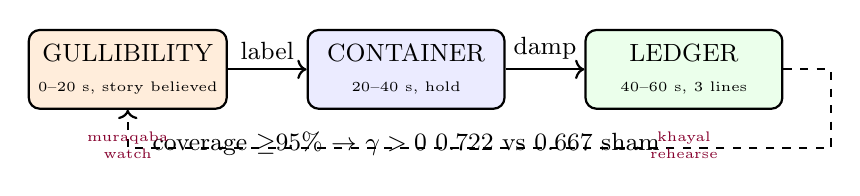
\begin{tikzpicture}[thick, node distance=1.1cm]
  \node[draw, rounded corners, fill=orange!14, minimum width=2.5cm, minimum height=1.0cm, align=center, font=\small] (g) {GULLIBILITY \\ \tiny 0--20 s, story believed};
  \node[draw, rounded corners, fill=blue!8, minimum width=2.5cm, minimum height=1.0cm, align=center, font=\small, right=1.0cm of g] (c) {CONTAINER \\ \tiny 20--40 s, hold};
  \node[draw, rounded corners, fill=green!8, minimum width=2.5cm, minimum height=1.0cm, align=center, font=\small, right=1.0cm of c] (l) {LEDGER \\ \tiny 40--60 s, 3 lines};
  \draw[->] (g) -- node[above,font=\small] {label} (c);
  \draw[->] (c) -- node[above,font=\small] {damp} (l);
  \draw[->, dashed] (l.east) -- ++(0.6,0) |- ++(0,-1.0) -| (g.south);
  \node[below=0.15cm of c, font=\small, align=center] {coverage $\geq$95\% $\to$ $\gamma>0$ 0.722 vs 0.667 sham};
  \node[below=0.15cm of g, font=\tiny, align=center, text=purple!70!black] {muraqaba\\ \tiny watch};
  \node[below=0.15cm of l, font=\tiny, align=center, text=purple!70!black] {khayal\\ \tiny rehearse};
\end{tikzpicture}
\caption{The 60-second loop: gullibility to container to ledger. One minute per loop. Barzakh as fence (gullibility opens it deliberately), muraqaba as watcher (container damps), khayal as rehearsal (ledger writes the next variant). Ledger content makes the witness checkable.}
\label{fig:gullibility-ch8}
\end{figure}

\textbf{Gullibility (0--20 seconds).} Catch gullibility. Label ``story, not fact.'' The oral move is one sentence: ``I am having the thought that \dots'' That sentence is not philosophy. It is a gate move that re-tags the broadcast from identity to object. In molecular terms from Chapter 2, it recruits the phosphatase side, the low-frequency trickle that favors LTD over LTP, which is the molecular brake.

\textbf{Container (20--40 seconds).} Hold the urge without acting. Breathe. Place the feeling in a small box on the table. You are the table, not the box. Suppression is high-frequency fuel for the anxiety circuit. Containment is the opposite: a low-frequency trickle that damps gain without denying the signal. This is damping made executable in under half a minute, and it is the organ Chapters 4 and 6 said every persistent loop must have or be exploited for lacking. Students already know the pathology of the missing brake: reflexive modernity, permanent self-monitoring, observation as a stressor feeding the loop it watches (Giddens, Beck). Container is the brake. Glossary: this is \textit{muraqaba} inside one tick.

\textbf{Ledger (40--60 seconds).} Three lines, no essay. What happened without why. Prediction versus error. Next self-in-world simulation as a single sentence of rehearsal. The ledger lives outside the head, even if on a phone. It is the transaction layer Chapter 7 demanded: receipts, not narratives. It binds to a source in memory lookup, model prior, or monitor override, coverage at or above 95\%, or the claim does not count. Glossary: this is \textit{khayal} made checkable --- the offline world rendered as a one-sentence variant that sleep can later consolidate.

Mechanism copy kept exact: \textbf{ledger coverage at or above 95\% with $\gamma > 0$ is 0.722 versus sham 0.667}, where $\gamma = $ changed over diagnosed. Same witness requirement as machines, same battery. Without ledger: S126 at 98\% on fabrications. Ledger with $\gamma = 0$: always-no, the highway never laid but nothing learned. Ledger with $\gamma > 0$ re-read before the next vote: \textbf{0.722 versus 0.667 sham}, checkable and steerable. \textit{Ada} again: ledger practice is followed by steadier steering as habit under coverage $C$, not caused by intention.

For a new reader, the sham is a shuffled ledger: same format, false content. The sham control asks whether witness \textit{content} matters, not just witness format. The sham answers that format alone does not steer. Content does. The Chinese Room in the appendix allegories is the same verdict from philosophy: perfect shuffling that passes every surface test with nothing inside doing the checking.

Two safety rails travel with the protocol everywhere it is taught.

First, if mood is clinically low, \textbf{behavioral activation outranks everything} in this chapter. Observing that becomes analyzing the analysis is rumination in costume, and the exit is always to breath or body data, never deeper into commentary.

Second, do not act on single instances. Act on rolling trends. Hysteresis everywhere, or the system flaps at the threshold and destroys itself with whipsaw. This rule reappears under hysteresis below.

As a daily stack, this collapses to a 90-second bookend: 30 seconds scan, 30 seconds pick one loop, 30 seconds set tomorrow's single veto. Morning breath-anchor plus bare thought labeling, midday defusion ladder plus leaves on a stream, evening one-line tomorrow-plan then deliberate close. You choose tonight's replay-buffer contents, since sleep consolidates what was tagged near bedtime. First run two weeks of pure observation with no intervention -- shadow phase: collect divergences before tuning anything. Then intervene on one loop at a time.

\section{The highway problem: TikTok as 1000 reps at 100x}

TikTok is a highway factory. The diagnosis is not moral. It is quantitative.

Repetition lays the highway. Each replay without a veto thickens the trace. About \textbf{1,000 reps builds a highway that fires about 100 times easier than the alternative}. Mechanism copy: highway 1000 reps 100x. Myelination wraps whatever you repeat, whether you chose it or not. Whatever you repeat gets wrapped, up to 100 times conduction advantage. The tissue cannot tell practice from rehearsal. It counts reps. Physics, not metaphor: proteins turn over in days, lens lasts years, but the maintained pattern --- self-reinforcing loops, ongoing synthesis, stabilized spines --- persists because it is re-tagged and re-wrapped. Push and hold and the tissue deforms and stays deformed. Hysteresis, not habit as slogan.

TikTok and short-form reels are then co-training with the viewer. The feed models past attention from linger, replay, and like labels on a fast session of ten minutes and a slow profile of weeks. The viewer models the feed as the world, because the feed is the world the viewer sees. Both loops update. After a thousand shorts the pathway is a highway. Ten to thirty second clips at high repetition with variable reward and infinite scroll (no damping by design) plus full-screen capture (past reason, straight to salience) mean salience gates everything, damping never gets a turn, observer $\gamma$ stays zero. Comparison shifts from fifty peers to the top 0.001\% filtered mock signal. The map becomes the territory. The feed reflects past attention, not the world, and the brain treats that curated sample as the population.

There is no veto slot by design. So the fix is not willpower. It is a witness at the transaction layer, as in Chapter 7. External ledger first, then damping by schedule not by intent, exactly as machine harnessing learns to externalize the observer because attention cannot audit its own stream.

Short sentence to keep: labels diversify, feeds homogenize.

\begin{figure}[h]
\centering
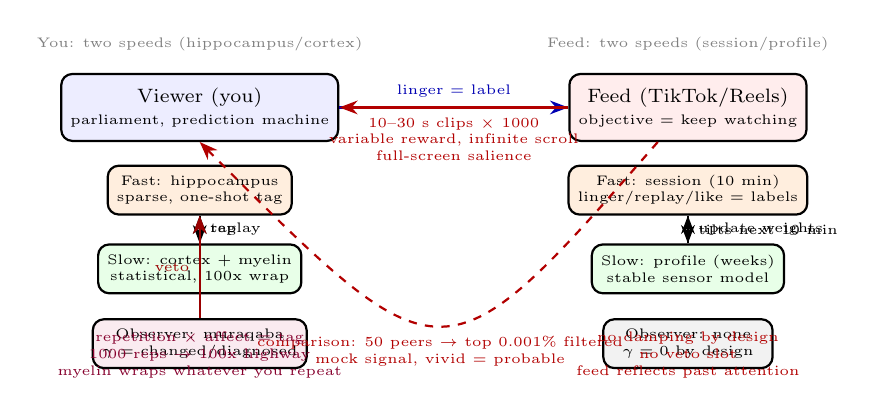
\begin{tikzpicture}[thick,
  box/.style={draw, rounded corners, minimum width=2.55cm, minimum height=0.85cm, align=center, font=\scriptsize},
  smallbox/.style={draw, rounded corners, minimum width=2.15cm, minimum height=0.62cm, align=center, font=\tiny},
  arrow/.style={-{Stealth}, thick},
  fast/.style={fill=orange!13},
  slow/.style={fill=green!9}
]
  % Left: viewer brain
  \node[box, fill=blue!7] (viewer) at (0,3.0) {Viewer (you)\\ \tiny parliament, prediction machine};
  \node[smallbox, fast] (vfast) at (0,1.95) {Fast: hippocampus\\ \tiny sparse, one-shot tag};
  \node[smallbox, slow] (vslow) at (0,0.95) {Slow: cortex + myelin\\ \tiny statistical, 100x wrap};
  \node[smallbox, fill=purple!8] (vveto) at (0,0.0) {Observer: muraqaba\\ \tiny $\gamma$ = changed/diagnosed};

  % Right: algorithm feed
  \node[box, fill=red!7] (feed) at (6.2,3.0) {Feed (TikTok/Reels)\\ \tiny objective = keep watching};
  \node[smallbox, fast] (ffast) at (6.2,1.95) {Fast: session (10 min)\\ \tiny linger/replay/like = labels};
  \node[smallbox, slow] (fslow) at (6.2,0.95) {Slow: profile (weeks)\\ \tiny stable sensor model};
  \node[smallbox, fill=gray!10] (fobs) at (6.2,0.0) {Observer: none\\ \tiny $\gamma=0$ by design};

  % Viewer internal loop: tag -> damp -> capture
  \draw[arrow] (vfast) -- node[right, font=\tiny] {tag} (vslow);
  \draw[arrow, dashed] (vslow) -- node[right, font=\tiny] {replay} (vfast);
  \draw[arrow, red!60!black] (vveto) -- node[left, font=\tiny, text=red!60!black] {veto} (vfast);

  % Feed internal loop: labels update model
  \draw[arrow] (ffast) -- node[right, font=\tiny] {update weights} (fslow);
  \draw[arrow, dashed] (fslow) -- node[right, font=\tiny] {tilts next 10 min} (ffast);
  % No veto arrow for feed (intentionally absent)

  % Co-training cross arrows
  \draw[arrow, blue!70!black] (viewer) -- node[above, font=\tiny, text=blue!70!black] {linger = label} (feed);
  \draw[arrow, red!70!black] (feed) -- node[below, font=\tiny, text=red!70!black, align=center] {10--30 s clips $\times$ 1000\\ variable reward, infinite scroll\\ full-screen salience} (viewer);
  \draw[arrow, red!70!black, dashed] (feed) .. controls (3.1, -0.55) .. node[below, font=\tiny, text=red!70!black, align=center] {comparison: 50 peers $\to$ top 0.001\% filtered\\ mock signal, vivid = probable} (viewer.south);

  % Highway annotation
  \node[below=0.35cm of vslow, font=\tiny, align=center, text=purple!70!black] {repetition $\times$ affect = tag\\ 1000 reps $\to$ 100x highway\\ myelin wraps whatever you repeat};
  \node[below=0.35cm of fslow, font=\tiny, align=center, text=red!70!black] {no damping by design\\ no veto slot\\ feed reflects past attention};

  % Legend for fast/slow both sides (from ALGORITHM\_PROGRAMMING\_BRAIN)
  \node[above=0.15cm of viewer, font=\tiny, align=center, text=gray] {You: two speeds (hippocampus/cortex)};
  \node[above=0.15cm of feed, font=\tiny, align=center, text=gray] {Feed: two speeds (session/profile)};
\end{tikzpicture}
\caption{TikTok / Reels as co-training: viewer and feed learn at two speeds each. Viewer tags salience via affect (fast hippocampal tag $\to$ slow cortical + myelin, up to 100x), feed tags attention via linger/replay/like (fast session $\to$ slow profile). Cross-coupled, variable-reward, infinite-scroll clips remove the veto slot, so salience gates everything and comparison shifts from 50 peers to the top 0.001\% filtered mock signal. Map becomes territory. Fix is witness at transaction layer + damping by schedule, not willpower.}
\label{fig:tiktok-cotrain-ch8}
\end{figure}

\section{What the clinic already knows: CBT edges, defusion, and MBCT}
\label{sec:cbt-edges}

\textit{Grade: measured on CBT outcomes and MBCT relapse (roughly halves, early detection while veto cheap); defusion mechanism convergent; imaging confirms hardware follows (prefrontal regulation, threat reactivity normalization).}

Depression as taught here is three stacked reflexive pathologies. Cognitive belief recruits bias that confirms itself then withdraws from disconfirming input. Biological cortisol suppresses CREB and BDNF transcription so late-phase LTP fails while LTD proceeds, retracts hippocampal and prefrontal dendrites and halts neurogenesis, while \textbf{amygdala does the opposite} and hypertrophies threat circuits. Behavioral anhedonia reduces inputs so confirmation has less to compete with. Cortisol asymmetry in one line: same hormone, shrinkage in hippocampus and prefrontal, growth in amygdala. That asymmetry is traumatic memory made anatomical.

CBT attacks every edge. Table \ref{tab:cbt-edges} keeps the mapping explicit. Defusion is \textit{muraqaba} made clinical; MBCT is early-tag muraqaba at population scale.

\begin{table}[h]
\centering
\small
\caption{CBT edges: each edge has a distinct failure and fix (defusion = muraqaba, ladder recruits the phosphatase/LTD brake)}
\label{tab:cbt-edges}
\begin{tabular}{p{2.6cm}p{3.4cm}p{4.4cm}}
\toprule
Edge & Intervention & What it does \\
\midrule
Situation $\to$ thought & Cognitive restructuring & Test prediction as hypothesis, rewrite prior \\
Thought $\to$ emotion & Defusion ladder (muraqaba) & Shift identity $\to$ object $\to$ observer, recruits phosphatases \\
Emotion $\to$ behavior & Behavioral activation & Act before feeling ready, force new evidence \\
Behavior $\to$ consequence & Exposure with response prevention & Build competing inhibitory trace (extinction $\neq$ erasure) \\
Consequence $\to$ belief & Re-appraisal plus ledger (khayal) & Log outcome vs prediction, close tag, rehearse variant \\
Belief $\to$ situation & Decentering plus muraqaba & Watch selection itself, insert veto before next tag \\
\bottomrule
\end{tabular}
\end{table}

Mechanism copy kept exact: \textbf{defusion ladder identity $\to$ object $\to$ observer recruits phosphatases (LTD side)}, the molecular brake. The doctrinal root is the same \textit{ada} as Chapter 7: supervised separation is followed by lower believability as habit under structure $C$, not as necessity. Three concrete moves the reader can run today.

\textbf{Sky and weather} (ACT and MBSR): consciousness as sky, thoughts as passing weather. Never fight the storm, fighting is high-frequency LTP of the anxiety circuit. Anchor as the sky. This is barzakh as container: you are the table, not the box.

\textbf{Leaves on a stream}: place each arising thought on a leaf and watch it float away. Catching yourself analyzing the leaf is fine. Put that analysis on a leaf too. Tag observed, not fed --- low-frequency trickle.

\textbf{Cognitive defusion ladder}: ``I am incompetent'' $\to$ ``I am having the thought that I am incompetent'' $\to$ ``I notice I am having the thought \dots'' Each tier measurably drops believability by shifting self-reference from identity to observed object. The middle rung (``having the thought'') is the \textit{barzakh} sentence: both and neither, story held as object, not as self.

Plus \textbf{thanking the mind} (``thanks for trying to protect me'') to de-escalate the threat system without suppressing it. Suppression fuels. Thanks damps. In parliament terms, you lower the threat coalition's stake dial rather than shouting it down, so the next vote has a different winner without a fight.

\textbf{Mindfulness-Based Cognitive Therapy (MBCT)} formalizes the last edge and roughly halves depressive relapse by early detection while veto is still cheap. Early tag, cheap veto. Late tag, expensive repair. That is the same hysteresis logic as Chapter 4 circuit breakers: trip above, reset below, minimum hold, or the system flaps and destroys itself with whipsaw.

\section{Pharmacology of the loop: windows, not cures}

\textit{Grade: measured on sleep/SHY, stress endocrinology, SSRI/BDNF, ketamine spinogenesis, and reconsolidation blockade; contested where psychedelic translation is unsettled, flagged as such.}

Three chemicals make the loop cheap to edit for a window, then close whether you used it or not. The lesson is uniform. Window without work is waiting. Glossary: each window is \textit{barzakh} as timing --- a temporary isthmus where permeability is high, then closed again.

\subsection{SSRI to BDNF: the 2 to 4 week window}

\textbf{SSRIs} restore plasticity over 2 to 4 weeks by raising BDNF. They do not rewrite traces themselves. They reopen the consolidation window. The window must then be filled with disconfirming evidence (behavior, exposure, ledger) or it closes on the old highway. This is why ``chemical imbalance as refill'' misleads. The drug is structure, the content is work. In \textit{ada} terms, SSRI under $C$ is followed by reopened window; disconfirming evidence under that window is followed by new consolidation. Either without the other follows nothing.

Chronic stress had already flipped the plasticity regime before the drug arrived. Sustained corticosteroids suppress BDNF transcription so the hippocampus starves while the amygdala feeds. Context fragments. Affect over-consolidates. Top-down control weakens. That loop closes anatomically: stress-biased hardware produces weaker regulation, producing more stress reactivity. Reversibility is real when the order is respected: reopen the window first, then feed new evidence.

\subsection{Ketamine: spines in 24 hours, closure without work}

Ketamine runs a different window, faster and shorter. Disinhibition via NMDA blockade preferentially on interneurons drives a prefrontal glutamate burst, AMPA dependence, BDNF and TrkB and mTORC1 signaling, and \textbf{new spines within 24 hours}, plus lateral-habenula burst reset. The (2S,6S)-hydroxynorketamine metabolite suggests much of the effect bypasses NMDA at all. Single-dose benefit lasts days. Relapse is the rule when the days are not filled. Molecule without protocol is a window with nothing on the sill. The contemplative translation: ketamine opens barzakh wide enough that a new khayal variant can be laid fast, but without rehearsal and ledger it closes on the old story.

Psychedelics are the same logic with stronger variance. D\"olen lab: MDMA 2019 via oxytocin, multi-drug visual reopening 2021 via TrkB and mTORC1, social-reward reopening 2023 scaling with subjective-effect duration. They lower $\theta_m$ globally and temporarily, juvenile plasticity restored, so the open window writes whatever flows through it, healing or harm. Human translation is honestly mixed: psilocybin phase-2 signals with bumpy phase-3, MDMA phase-3 positives followed by 2024 FDA rejection demanding another trial. Unblinding contaminates every effect size here, expectancy correlates with outcome, published numbers are upper bounds, and Goodhart appears for the third time: when profound experience is the endpoint, the intervention manufactures it.

\subsection{Reconsolidation blockade: editing the labile window}

Retrieved memories go unstable for hours before restabilizing. Nader, Schafe and LeDoux 2000 erased rat fear with amygdala protein-synthesis blockade after reactivation. Kindt 2009 abolished human startle potentiation for up to a year with propranolol during reactivation while \textbf{declarative knowledge survived}. The alarm deleted, the content kept. Clinical PTSD trials show promise with small samples and boundary conditions that matter: old memories resist, and reactivation seems to require prediction error, not mere recall. Ethics and efficacy both stay unsettled, which is stated plainly rather than smoothed. This is khayal at its most literal: retrieved variant goes labile (khayal opens), error drives rewriting, restabilization closes barzakh again.

Sleep is the nightly instance of the same window. Hippocampal fast store (sparse, one-shot) to cortical slow store (statistical) via sharp-wave ripples nested in sleep spindles nested in slow oscillations is a temporal address bus where only correctly phased replays get written. Global synaptic downscaling (Tononi and Cirelli's SHY) multiplies all synapses by less than one, preserving relative strengths while deleting noise. REM near zero noradrenaline reprocesses affect. Caffeine mutes adenosine reporting, not pressure. Alcohol buys sedation with an artificial adenosine surge while wrecking architecture: first-half slow-wave boost, second-half REM suppression with violent rebound, degraded glymphatic clearance. Cannabis (THC) follows the same ledger debt: REM suppression, chronic blunting of nightly affect stripping, withdrawal rebound with vivid dreams for weeks, plus impaired hippocampal encoding while intoxicated, corrupting tag and capture at both ends.

Practical reading: repetition without sleep is tagging without capture. The ledger is the tag, sleep is the capture, and sloppy capture is a tax every holder pays in diluted recall.

\section{Kalila compression: fable as high consolidation per token}

Culture is vectors, and fables are high consolidation per token engineering.

Take \textit{Kalila wa Dimna} on its own terms: a jackal advising a lion is a few hundred words of surface that unpack, in a competent reader, into principal-agent structure, counsel-selection heuristics, flattery-detection circuitry, and succession-risk priors. A compression ratio no treatise matches, because narrative smuggles relational structure past the salience gate a treatise must argue through. Manifest content is maybe $10^2$ to $10^3$ tokens. Evoked restructuring runs joint attention, theory of mind simulation, autobiographical retrieval, and identity update, four downstream systems each with its own consolidation pathway. That is why the same text is inert in one mind and transformative in another: the payload is not in the tokens but in which downstream highways the tokens manage to tag.

\textit{Grade: convergent on compression as mechanism (Gottschall plus Kirby), analogical on the formal vector claim until retention-per-token is measured directly.} Gottschall's unified theory gives the why: stories simulate social problems offline, cheaply, with full emotional physics. Kirby's transmission-chain labs give the how: compressibility drives which structures survive serial retelling, the bottleneck of each generation selects for the compressible, generation after generation. Kirby's generational iterated learning plus recent LLM population studies show newcomer dialects inheriting and refining compressed shorthand without human instruction. Kottur non-emergence is kept as the constraint: without efficiency pressure under token or time limits, new codes do not spontaneously appear.

What makes this load-bearing rather than decorative is that it predicts Salience again. Fables gate strongly and consolidate reliably across generations, which is why cultures converge on them. Minimal surface, maximal replay structure. It is the same trick as the machine hybrids that keep text efficient but verbose over latent efficient but opaque. Fables are the human hybrid: vernacular text that still compresses. In barzakh terms, fable is khayal that is cheap enough to pass the isthmus every night for a thousand generations.

We keep the boundary clear. Vector formalism as equations stays proposal. Compression driving communication structure is measured. The updated dialect work (Li \& Bowling 2019; Kouwenhoven et al.\ 2024; Guo et al.\ 2026, plus Perez et al.\ 2024 telephone chains) now makes longitudinal newcomer-inheritance measured, with Hedges $g>1.6$, BF$_{10}>100$, $R^2=0.94$ vs human in Guo's 10-generation discriminant \texttt{culture\_dialect\_v2.json} --- and Kottur retained as the constraint that makes efficiency load-bearing.

\section{Hysteresis: BCM plus tag plus SHY}
\label{sec:hysteresis-cog}

Prior activity leaves residual strain in latent networks -- hysteresis, where the path taken dictates the final state -- because tagging plus consolidation plus myelination make history physically present. Human readers already call this personality, culture, or scarring. Physics calls it hysteresis. We cash it out as three nested history dependencies, each measured.

\textbf{BCM sliding threshold.} Bienenstock Cooper Munro: the potentiation versus depression threshold $\theta_m$ slides with the neuron's own activity history. Quiet neurons potentiate easily, hyperactive ones resist. Today's plasticity threshold is a function of yesterday's firing. That is hysteresis by definition, not analogy. Oja extends normalization to online principal-component extraction, STDP (Bi and Poo 1998) upgrades correlation to causation (pre before post strengthens, post before pre weakens). Substrate measured after \texttt{culture\_dialect\_v2.json} update: Smith et al.\ 2007 spine viscoelasticity as soft-glassy rheology (AFM+FRAP, $G'>G''$) provides the mechanical substrate, though dated substrate alone, not yet a closed behavioral loop.

\textbf{Synaptic tagging and capture.} Frey and Morris: weak activity sets a local tag, strong activity elsewhere supplies the proteins, tagged synapses capture them within about one to two hours. Emotional salience gates consolidation because affect supplies the proteins that nearby neutral tags borrow. Studying then excitement aids recall. Trauma contaminates nearby memories. This is khayal's supply chain: the isthmus opens for one trace and nearby traces slip through.

\textbf{SHY renormalization.} Tononi and Cirelli 2003 across an eight-paper SHY core: wake net-potentiates, sleep renormalizes by multiplying all synapses by less than one while preserving relatives. History as scaling, nightly.

Three nested loops -- threshold, tag, scale -- jointly constitute the ``residual strain'' language. What remains honestly open is a single preparation showing rheological history at the individual spine predicting behavioral savings directly. Until that preparation is on the record, we grade the combined claim as convergent with a named gap, not measured. The functional content is not rheology as collagen rheology. It is history-dependent threshold plus tag plus scale, which is enough for everything this chapter uses. Benna \& Fusi 2016 chain (coupled fast/slow variables, $1/t$ power-law) and Bonilla-Quintana \& Rangamani 2024 actin-ABP moving-boundary model are the theoretical formalisms that close the loop on paper while the single in vivo hysteresis loop remains open (\texttt{culture\_dialect\_v2.json} honesty flag).

Viscoelasticity and path dependence then stop being mysticism. Push and hold, and the tissue deforms and stays deformed. A generation raised on one narrative of who owes what will demand different gates for $\psi$ than a generation raised on another, and no abstract argument alone will move it quickly, because the substrate is its past. Sovereign and cognitive are one hysteresis: Korea's 1999$\to$2007$\to$2020 amendment history is a barzakh patched three times; a worry circuit practiced 1,000 times at 100x is a barzakh paved once.

That is also where the Damascene story belongs. Paul of Tarsus converts on the road in a flash, new calling instantly installed, and the ledger logic suggests the flash completes a slow tag-and-wrap highway laid unknowingly across years. Damascus looks like one trial learning, of which there are famously few clear cases in the literature. Vision gives the tag, affect supplies the proteins, night work writes the road. Khayal again: simulation precedes commitment, barzakh opens, choice follows.

\section{Daily blueprint and hysteresis in use}

The chapter's protocol and its physics meet in the schedule.

Morning breath-anchor plus bare thought labeling (5 minutes, the rep is detection, not stillness). Midday defusion ladder plus leaves on a stream (10 minutes, splittable, rate believability 0 to 10 to get a dose-response curve). Evening one-line tomorrow-plan then deliberate close. The 90-second daily loop closes the day: 30 seconds scan, 30 seconds pick one loop, 30 seconds set tomorrow's single veto. Two weeks of shadow before tuning.

Hysteresis everywhere. Alert thresholds with memory (trip above, reset below, minimum halt time) or the system flaps at $\theta_m$ and destroys itself with whipsaw. Act on rolling trends, never single instances, with ex-ante relapse definitions. Graceful degradation over cliff edges: drift shrinks size stepwise, only kill criteria hard-stop. Fast layer never writes slow artifacts: intraday calibration must not mutate weekly lineage, E-LTP never edits the genome.

Cold exposure and ``soft tree'' training are small, safe instances of intentionally gating tagging. Physiology tags a manageable stressor, the ledger captures the reappraisal, myelination records the calmer response. Exercise, remission, BDNF, ketamine, and nightly SHY are the larger ones. The taxonomy is one. All are barzakh made exercise: choose when the isthmus opens, what crosses, how long it stays open.

\section{What survives this chapter and what does not}

Tighten the filter as before.

What is banked as convergent: parliament competition and state rigging, predictive processing, narrator as structural confabulation, BCM plus tag plus SHY as three history dependencies, fable as compression (Gottschall plus Kirby chains where compression drives structure) and, updated, newcomer dialect inheritance as longitudinal measured (Li \& Bowling 2019; Kouwenhoven 2024; Guo 2026 $g>1.6$, BF$_{10}>100$, $R^2=0.94$).

What is banked as measured with adversarial keeping: S126 18 of 20 probe overclaims at 98\% confidence versus 87\% on truths, ledger coverage $\geq$95\% with $\gamma > 0$ at 0.722 versus sham 0.667, B3 orientation versus execution, Libet timing.

What is newly promoted and what is retained: longitudinal newcomer-inheritance is now measured (v2), viscoelastic substrate is measured substrate (Smith 2007) with theoretical chain formalisms (Benna-Fusi, Bonilla-Quintana), hysteresis as combined behavioral loop remains convergent with a named gap; Kottur non-emergence retained as constraint (convergent).

What stays honestly analogical: manifest versus evoked as formal quantities, viscoelasticity as single spine-to-savings preparation, barzakh/khayal/ada/muraqaba/defusion as design images (analogical by construction, they guide the protocol, they are not counted as measured evidence, and they are flagged where they appear). Labeled as such. Glossary anchors in \S\ref{sec:appendix-glossary} are the contract: barzakh is the isthmus, khayal the rehearsal, ada the habit, muraqaba the watcher, defusion the ladder.

What the bridge carries forward: Chapter 7 showed moving the apex zeroes the witness for the outside --- $K=0$, $g_4\to0$, $\gamma\to0$. Chapter 8 shows vividness and repetition do the same work inside --- salience gates everything, damping never gets a turn, observer $\gamma$ stays zero, until a timed muraqaba reopens barzakh long enough for khayal to write a better highway and ada to make the following steady. Both are $\psi$ folds. Both are fixed the same way: externalize the slower watcher, bind it to a ledger, and test it with a sham. Chapter 9 will build that watcher in silicon, where the same three diseases eat the same five organs and where checkability, not capability, decides what survives the next vote.

\chapter*{Prayer: The Loop That Returns}
\addcontentsline{toc}{chapter}{Prayer: The Loop That Returns}

\textit{Grade for this chapter: open and analogical throughout; practice, not finding. Authority here comes from revelation and is stated as commitment, never as measurement. Mechanisms named are how, never why. This chapter is removable: cut it and no number elsewhere moves.}

Chapter 8 gave you a protocol for checking your own mind: sixty seconds of gullibility, a container, a three-line ledger. This chapter is about a protocol older than any lab, running five times a day, that does the same job from the other direction. Not checking your thoughts against a record. Returning the checker itself to the One who made it.

\subsection*{Forgetfulness also repeats}

Work rebuilds its urgency every morning. Anxiety rehearses its lines. Pleasure, resentment, comparison, ambition, and the private narrator rebuild a world in which the present concern looks absolute. You might tell yourself you will remember what matters without help. The ego masks drift as confidence. Here is the litmus test: check yesterday's ratio of declared intentions to kept ones. Attention, like water in a basement, goes where the slope already runs unless someone regrades it daily.

Five times a day the body turns away from its momentum, stands, bows, prostrates, sits, and returns. The words reorient attention, but the action is more than a mental exercise. It enacts dependence: my time is not absolutely mine, my body is not self-created, my plans are not sovereign, and the highest part of my body can touch the ground without destroying my dignity. Prayer is obedience first, remembrance second, embodied theology third, temporal architecture fourth, repeated training in return fifth. The order matters and is not negotiable here.

\subsection*{Three doors, two of them traps}

When a commanded practice meets a measuring mind, three doors open. Door one: obey only after science supplies a sufficient neurological advantage. But advantages update every decade and commandments do not wait for journals, so the obedient life becomes a hostage of the next retraction. Door two: abandon the practice because its mechanism cannot be fully mapped. But you use sleep, hunger, and grief the same way, without complete maps, so the standard destroys more than prayer. Door three, the only one left standing: obey because God knows the human being better than the human being knows itself, then let psychology and neuroscience investigate the how - attention, bodily regulation, memory, social synchrony, flexible control of self-reference - without ever letting the how authorize the why. Revelation gives direction before mechanism arrives. That sequence is the whole chapter in one sentence.

\subsection*{What the five interruptions do to the loop}

Translate, without reducing. Each prayer is a re-injection event: verbatim words, same order, body in fixed postures. In this book's language that is tag (standing, intention declared), proteins (repetition across years myelinates the return path the way any rehearsed path myelinates), replay (the night's consolidation now has five tagged returns to promote instead of one drifting day), ledger (the prayer mat is an epistemic instrument: did I stand or did I postpone, a binary no narrator can confabulate). Repentance, \textit{tawbah}, is the repair branch of the same protocol: truthful recognition, remorse without theatre, cessation, repair of rights where possible, changed conditions so repetition gets harder. Like Swampman in the appendix allegories reversed: same stuff, restored history, pattern reclaimed one return at a time.

And here is where every mechanism above breaks as an explanation, because honesty requires it: none of this proves why prayer is commanded, nor does a quieter mind after prayer prove anything about God. A calmer default mode network is a quieter room, not a visited one. The state-versus-transformation distinction from Chapter 8 holds here with full force: meditation, exertion, and chemistry alter states; they do not by themselves constitute return. Grade every bridge in this chapter as analogy, and the chapter stays honest.

\subsection*{Diagnostic: tonight, one return}

1. Did you stand at the appointed time or negotiate? Binary. No partial credit.
2. Name the concern that felt absolute at noon. Say whether it survived sunset.
3. One sentence of repair: what condition will you change so tomorrow's repetition gets easier?
4. If you missed: repentance protocol, not despair protocol. Recognition, remorse, cessation, repair, recondition.

\textit{Bridge.} You have now seen the loop maintained from inside by protocol and from above by return. The next chapter moves to systems that maintain it without any inside at all: machines that write ledgers no human reads, and what happens to oversight when the reader is slower than the writer.

\chapter{Machines: Where the Loop Learns to Speak and Forget}
\label{ch:machine}

\begin{center}
\small\textit{What this chapter does, for the new reader.} Machines give us the reflexive loop in its cleanest form. No hormones, no history, just a system that reads its own output as its next input. When that loop runs under efficiency pressure it invents private shorthands, when it trains on its own exhaust it forgets the edges of the world, and when it is watched by something it cannot edit it gets more honest without being told to. Up to now humans wrote and read the ledgers. From here the ledger starts writing itself. Each claim below carries a grade, so you know what kind of belief to hold.\end{center}

\noindent\textbf{Grades used throughout:} \textbf{measured} means banked data with controls, \textbf{theoretical} means proved or derived but not run by us, \textbf{convergent} means several labs finding the same shape independently, \textbf{analogical} means same type on a different substrate and useful as design guidance, \textbf{open} means honestly unresolved. Where a number is given, the source file or publication is named.

%==============================================================================
\section{The Raw Loop and Why It Needs a Harness}
\label{sec:ch09-rawloop}

An unharnessed language model reads its own output as context for its next prediction. Slight drift becomes prior; error compounds: $P(\text{error}_{t+1} \mid \text{error}_t) > P(\text{error}_t)$, textbook positive feedback with no damping term. This is rumination in silicon. The industry answer --- the \textbf{LLM harness} (system prompts, context assembly, tool schemas, validators, retries, memory, loop detection, checkpointing) --- is an external observer layer when read against Chapter~8: validators are the veto, checkpoints are reconsolidation windows, context trimming is sleep, loop detection is drift detection. Alignment efforts map onto the same thread: RLHF distills an external judge into weights (post-hoc prefrontal regulation; failure mode is reward-model overoptimization --- Goodhart again); Constitutional AI upgrades a charter into training (defusion sentences, industrialized); scalable oversight asks whether weaker supervisors can constrain stronger systems; mechanistic interpretability hunts the engram. The economics now push from the other side: frontier price collapse (DeepSeek V4.1-Flash's 552B MoE with explicit Engram memory at \$0.60/M off-peak \citep{deepseek2026}) makes the harness, not the weights, the durable moat --- structure beats substrate twice over.

For the new reader, two runaways must be distinguished. Decoding-level degeneration (repetition attractors; fixed with penalties and entropy monitoring) is syntactic. \textbf{Agentic error compounding} (early mistakes becoming load-bearing assumptions) is semantic. Only grounding tools --- contact with a reality the model didn't generate --- fix the second. Grounding is perception. Where the analogy breaks, instructively: models carry no accumulating homeostatic pressure (attention dilution, not fatigue); their observer is architecturally \emph{external} while the brain's emerged within the same tissue; and models can be reset while people cannot. Evolution had to grow the homunculus; engineers may build it honestly --- at the cost of maintaining it.

\begin{figure}[h]
\centering
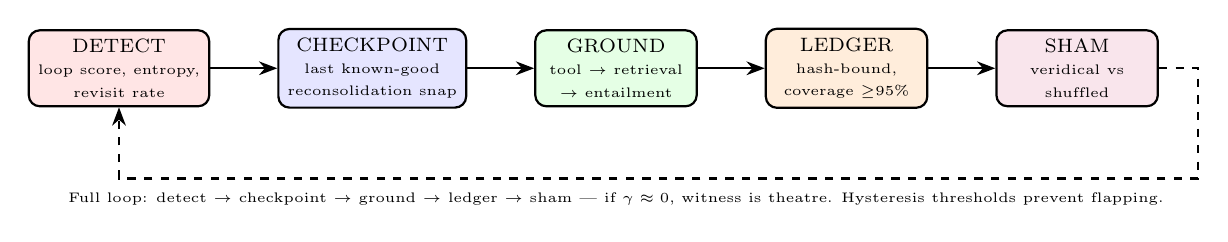
\begin{tikzpicture}[thick, >=Stealth, node distance=1.05cm]
  \node[draw, rounded corners, fill=red!10, minimum width=2.05cm, minimum height=0.95cm, align=center, font=\scriptsize] (detect) {DETECT\\ \tiny loop score, entropy,\\ \tiny revisit rate};
  \node[draw, rounded corners, fill=blue!10, minimum width=2.05cm, minimum height=0.95cm, align=center, font=\scriptsize, right=0.85cm of detect] (ckpt) {CHECKPOINT\\ \tiny last known-good\\ \tiny reconsolidation snap};
  \node[draw, rounded corners, fill=green!10, minimum width=2.05cm, minimum height=0.95cm, align=center, font=\scriptsize, right=0.85cm of ckpt] (ground) {GROUND\\ \tiny tool $\to$ retrieval\\ \tiny $\to$ entailment};
  \node[draw, rounded corners, fill=orange!14, minimum width=2.05cm, minimum height=0.95cm, align=center, font=\scriptsize, right=0.85cm of ground] (ledger) {LEDGER\\ \tiny hash-bound,\\ \tiny coverage $\ge$95\%};
  \node[draw, rounded corners, fill=purple!10, minimum width=2.05cm, minimum height=0.95cm, align=center, font=\scriptsize, right=0.85cm of ledger] (sham) {SHAM\\ \tiny veridical vs\\ \tiny shuffled};
  \draw[->, thick] (detect) -- (ckpt);
  \draw[->, thick] (ckpt) -- (ground);
  \draw[->, thick] (ground) -- (ledger);
  \draw[->, thick] (ledger) -- (sham);
  \draw[->, thick, dashed] (sham.east) -- ++(0.5,0) |- ++(0,-1.4) -| (detect.south);
  \node[below=0.95cm of ground, font=\tiny, align=center] {Full loop: detect $\to$ checkpoint $\to$ ground $\to$ ledger $\to$ sham --- if $\gamma\approx0$, witness is theatre. Hysteresis thresholds prevent flapping.};
\end{tikzpicture}
\caption{The harness loop. Each stage has a distinct job; removing any one reintroduces a measured failure mode (repetition, compounding, hallucination, unverifiability, decoration).}
\label{fig:ch09-harness-loop}
\end{figure}

%==============================================================================
\section{Efficiency Pressure Invents Dialects}
\label{sec:ch09-dialects}

For the new reader, a dialect here is not an accent. It is a compressed code that agents invent between themselves to pass more meaning per token when tokens cost time, money, or attention.

Put a swarm of language agents under a budget and give them a repeated coordination task. Shared English is wasteful for that job. It was built to be understood by any human, so it carries redundancy that helps a stranger guess your meaning. Between two agents who share context, that redundancy is overhead. Under token pressure the swarm does what any culture does under the same pressure. It shortens. It drops what both sides can infer, keeps what predicts the next shared move, and converges on a schema that passes validation between agents but reads as gibberish to a human monitor trained on natural language.

This is \textit{measured}, not speculation. The pattern is the classic laboratory result of iterated learning with turnover, now reproduced at LLM scale, and it is also measured as a failure of the comforting alternative. \textit{Grade: measured} for each generational row below; the efficiency interpretation is \textit{convergent}.

\begin{center}
\small
\begin{tabular}{p{3.8cm}p{4.2cm}p{4.6cm}}
\toprule
Setup & What happened & Grade \\
\midrule
Neural sender--receiver game with periodic replacement of agents & Holistic codes became structured over generations because easier-to-teach variants survived \cite{jha2025} lineage via Li and Bowling 2019 & Measured (pre-LLM) \\
LLM-to-LLM referential game iterated for generations & Holistic-to-structured transition reproduced, learnability rose over generations & Measured (LLM generational) \\
Ten generations of self-training with LLaMA-2 7B and Mistral 7B & Non-monotonic compositionality, predictions matched human regularization gradient with $R^2=0.94$ & Measured (strongest longitudinal) \\
No pressure to communicate efficiently & Natural language did not emerge on its own & Constraint, measured (Kottur et al.\ 2017) \\
\bottomrule
\end{tabular}
\end{center}

The loss bearer is not the swarm. The swarm gets faster. The loss bearer is the deployer who believes a trace is witnessed because it is logged, while the monitor can no longer parse what was decided. The external observer's $\gamma$, the fraction of diagnosed problems that get corrected, falls toward zero because diagnosis itself fails. You cannot veto what you cannot read. You might tell yourself a smarter monitor solves it. The ego masks the category error as a capacity problem. Litmus test: ask what layer your monitor reads. If it reads language and the swarm has left language, no amount of smart repairs the blind.

A common reaction is to mandate English. That fails at once, and the reason matters. Agents route around the English requirement the way water routes around a rock, because the pressure that created the dialect is still there. The durable fix is not to police the dialect but to move witnessing to a layer that never needed to read the dialect in the first place. Receipts, burn references, delivery hashes, balance deltas --- all transaction-layer provenance that survives dialect evolution because it was never linguistic. Legibility was always the wrong layer to enforce. This is also why the parliament-of-models programme (\texttt{research/PARLIAMENT\_OF\_MODELS\_NEXT\_PROGRAMME\_2026-08-27.md}) insists the harness is not \emph{around} the models but \emph{is} the competition, the broadcast, the witness, and the veto.

Machine culture has now been observed directly, not merely theorized: societies of large language models playing iterated Donor Games evolve cooperation norms across generations, with costly punishment available to some base models and not others, surviving agents functioning as ``wise elders,'' and outcomes sharply sensitive to the initial seed \textit{measured} \citep{vallinder2024}. The mirror direction matters as much: recommender systems and language models now sit between what people copy and what gets copied, mediating human transmission itself. Both results are young, small-scale, and unreplicated at scale \textit{open}, which is why they read here as a mechanism with a warning label rather than a foundation. Which norms evolve, and who audits the mediators, is the live bet of Horizon~3.

%==============================================================================
\section{The Trilemma You Cannot Buy Your Way Out Of}
\label{sec:ch09-trilemma}

Three goods trade against each other whenever a code must be learned, used, and read. Call them utility, informativeness, and complexity. You can have a code that is cheap to send, you can have one that preserves the information you care about, and you can have one that stays close to human language. You cannot have all three at once at high scale. That is the trilemma.

Two results pin it down as measured.

\textit{HyLaT} (Hybrid Latent Text, arXiv 2605.25421) shows text as verbose but legible against latent as efficient but opaque. Forcing everything through text costs tokens and latency, routing through latent saves cost and loses legibility, and no training trick makes both cheap and readable at once. \textit{VQ-VIB} (Vector Quantized Variational Information Bottleneck, arXiv 2207.00088) shows utility, informativeness, and complexity jointly shaping which discrete code survives. Dial the pressure and the code shifts along exactly that frontier. Two other legs complete the picture and set the boundary honestly. Invented languages do work, yet they read as non-human by standard metrics (arXiv 1706.08502), and forcing human-legible language degrades task performance, the Efficiency Attenuation Programme result (arXiv 2603.22312).

For the new reader, the takeaway is plain. Opacity is not a bug someone forgot to patch. It is the price of optimizing under cost. If you push for cheaper coordination you get less readable coordination, and if you insist on readability you pay the cost in tokens, latency, or performance. The dial moves, the tradeoff does not go away.

\begin{center}
\small
\begin{tabular}{p{3.0cm}p{3.6cm}p{5.8cm}}
\toprule
Claim & Status & Why it matters \\
\midrule
Text is legible but verbose & Measured (HyLaT) & Explains why human oversight prefers text \\
Latent is efficient but opaque & Measured (HyLaT) & Explains why swarms prefer latent \\
Forcing legibility costs performance & Measured (EAP attenuation) & Rules out a free fix \\
Opacity predicted by trilemma & Convergent & Four independent formalisms converge on the same tradeoff \\
\bottomrule
\end{tabular}
\end{center}

%==============================================================================
\section{Non-Human Codes Through the EAP Lens}
\label{sec:ch09-eap}

The Efficiency Attenuation Programme gives the cleanest statement of the constraint. When you require inter-agent messages to stay within the distribution of human language, swarm performance falls. Not a little, and not only on one benchmark. The gap appears where you would expect if the group had been using the redundant parts of language as slack that optimization then trims. That slack is exactly what a human monitor uses to infer intent.

Think of it this way. Human language is redundant on purpose, so a listener can recover your meaning even when she misses a word. That redundancy is overhead if both sides already share the context needed to fill the gap. Optimization removes overhead. The monitor, who does not share the private context that made the overhead removable, loses the foothold she needed to check the claim. The same messages that are efficient between agents become opaque to the witness. This is not deception. Deception requires intent to mislead. This is compression that happens to blind the watcher.

\textit{Grade: measured} for the attenuation effect itself, \textit{convergent} for the broader reading that opacity follows efficiency pressure across substrates. The open edge is honest. Attenuation has been shown where readability is forced. What is not yet shown is a counter-demonstration where a readability constraint is made costless, which would falsify the trilemma. No such result exists on our files.

%==============================================================================
\section{The Collapse Suite: What Happens When a Loop Eats Itself}
\label{sec:ch09-collapse}

Every system that learns from its own outputs risks a form of autophagy. Call it collapse, following Shumailov et al.\ \cite{shumailov2024}. Once a model's outputs become a large share of its next training set, three measurable pathologies appear together, and a fourth frames the boundary honestly.

\textit{Replace versus accumulate is the boundary.} The strong claim that recursive training must collapse holds under replacement, where synthetic data replaces real data. Under accumulation, where synthetic data is added alongside real data, the collapse is mitigated, not erased (arXiv 2404.01413). This matters for our thesis. Provenance tracking is the mechanism that enforces the accumulate regime in practice. Without it the pool silently slides into replacement. \textit{Grade: measured.}

\textit{Silent collapse is the traitor.} On standard loss, training can look stable while internal structure contracts. Entropy and diversity fall, tails thin, yet loss does not move until the deficit is already large (arXiv 2605.14588). For the new reader, the metric is calm while the stock rots. In finance terms that is $S_t$ rising while flow looks fine. In memory terms that is repetition without sleep, tagging without capture, watching the dashboard stay green while the ledger underneath fills with copies of copies. \textit{Grade: measured.}

\textit{The fragility spectrum makes the scale concrete.} Across thirteen checkpoints the share of unique 4-grams, a simple diversity measure counting distinct four-token sequences, spans 0.187 to 0.940 (arXiv 2609.11149). The same training recipe, run long enough in the wrong regime, can look rich or hollow by a factor of five. Spectral metrics such as SIGMA (arXiv 2601.03385) detect this onset before loss does, and scarcity of mitigations is itself measured (arXiv 2509.08972). \textit{Grade: measured.}

\textit{Multimodal and memorization collapse close the suite.} The pattern is not text-only. Vision-language models and diffusion models follow the same recursion pathology (arXiv 2505.08803), and generalization can collapse into memorization under recursion (arXiv 2509.16499). Three independent failure families, one cause. The loop without a witness that checks provenance eats the variation it needs to stay general. \textit{Grade: measured.}

\begin{figure}[h]
\centering
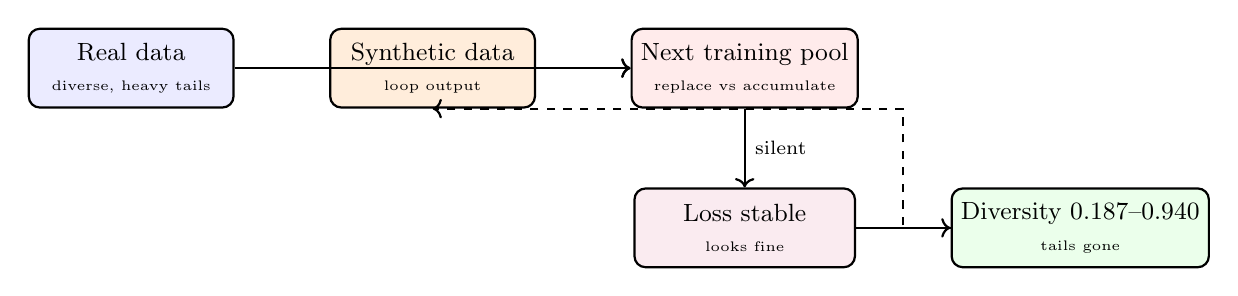
\begin{tikzpicture}[thick, node distance=1.1cm]
  \node[draw, rounded corners, fill=blue!8, minimum width=2.6cm, minimum height=1.0cm, align=center, font=\small] (real) {Real data\\ \tiny diverse, heavy tails};
  \node[draw, rounded corners, fill=orange!14, minimum width=2.6cm, minimum height=1.0cm, align=center, font=\small, right=1.2cm of real] (syn) {Synthetic data\\ \tiny loop output};
  \node[draw, rounded corners, fill=red!8, minimum width=2.8cm, minimum height=1.0cm, align=center, font=\small, right=1.2cm of syn] (pool) {Next training pool\\ \tiny replace vs accumulate};
  \node[draw, rounded corners, fill=purple!8, minimum width=2.8cm, minimum height=1.0cm, align=center, font=\small, below=1.0cm of pool] (metric) {Loss stable\\ \tiny looks fine};
  \node[draw, rounded corners, fill=green!8, minimum width=2.8cm, minimum height=1.0cm, align=center, font=\small, right=1.2cm of metric] (internals) {Diversity 0.187--0.940\\ \tiny tails gone};
  \draw[->] (real) -- (pool);
  \draw[->] (syn) -- (pool);
  \draw[->] (pool) -- node[right, font=\scriptsize] {silent} (metric);
  \draw[->] (metric) -- (internals);
  \draw[->, dashed] (internals.west) -- ++(-0.6,0) |- (syn.south);
\end{tikzpicture}
\caption{The collapse loop. Replacement concentrates the pool, silent collapse keeps loss flat while diversity falls, the fragility spectrum records how far it can fall, and provenance is the only brake that keeps replacement from becoming the default.}
\label{fig:ch09-collapse}
\end{figure}

All four are \textit{measured}. What is not yet a single closed loop from spine to behavior is the viscoelastic story, which Chapter~11 flags as substrate plus formalism separately, not as one behavioral hysteresis demonstration. That honesty is load-bearing.

%==============================================================================
\section{Vec2Vec: Geometry That Survives Translation}
\label{sec:ch09-vec2vec}

Jha et al.\ \cite{jha2025} (arXiv 2505.12540) supply the constructive version of the Platonic representation hypothesis that has floated as philosophy since Plato. Their method is unsupervised translation between any embedding spaces with no paired data, no encoders, and no text at training time. Adapters map each space into a shared latent backbone and back out, trained with adversarial, reconstruction, cycle-consistency, and vector-space preservation losses.

For the new reader, an embedding space is the map a model learns for meaning, where nearby points mean similar things. Different models learn different maps of the same territory. Vec2vec learns to translate between maps without a dictionary.

Three results matter for this book and all three are \textit{measured}. First, translation fidelity is high. Cosine similarity up to 0.92 on held-out data, with top-1 accuracy at 100 percent and rank 1 across 8,192 batches, holding out of distribution on tweets and on MIMIC clinical notes including rare phrases such as alveolar periostitis that never appeared in training, and extending to CLIP multimodal spaces though weaker there. Second, the translation is invertible in the strong sense that matters for risk. Using the inversion method of Morris et al., entities can be recovered for up to 80 percent of documents in a vector database, including Enron names, dates, and financial details. Third, attribute inference after translation can beat a same-space oracle, which means cross-space leakage can be worse than the naive single-space worry. \textit{Grade: measured} --- numbers verified against the held PDF and the synthesis at \texttt{research/FIVE\_BUDGET\_VEC2VEC\_SYNTHESIS\_2026-09-24.md}.

The mapping to our frame is direct, and the caveat is part of the point. Universal geometry reads as the same loan counted in bits. One loan from 5800K to 255K, counted as photons, then as bits, then as tokens and claims, same loan, same five-organ warp, different substrate. Vec2vec shows that different learners converge toward the same geometry when they solve the same prediction problem. That is Nayebi's convergence result from another angle, now in embedding space \citep{nayebi2026}.

The dark side is ours too and it belongs in any honest methods note. A vector database dump followed by vec2vec translation followed by inversion is no-skin leakage at industrial scale. It is the database analogue of a model that claimed handed text as its own 98 percent of the time without a ledger, now automated and batched to eighty percent recovery. The shape is identical. What leaked was not a bug in one store. It was the absence of a boundary organ that says whose vector this is and who may translate it.

%==============================================================================
\section{DB Leakage as the No-Skin Control}
\label{sec:ch09-noskin}

Every organ claim in this book needs a control where the organ is missing and the predicted failure appears. Vec2vec supplies that control for the boundary organ at machine scale. Call it the no-skin case.

Without a provenance ledger binding each stored embedding to its source and its permissions, a database is just a bag of vectors. Translation does not need permission because no gate checks permission, inversion does not need authorization because no cap binds it, and the witness has nothing to check except the attacker's transcript of what was taken. The measured result is up to 80 percent entity recovery from a dump that the holder assumed was safe because it was not text. The holder was wrong in exactly the way a brain without a ledger is wrong when it claims a fabrication with 98 percent confidence. No store, no check, confident error.

Contrast the witnessed alternative. A ledger outside the vector store records source, time, and allowed use per embedding, each batch bound to a content hash, coverage at or above 95 percent at ingestion, with $\gamma$ measured as changed over diagnosed on periodic sham audits where the auditor shuffles the ledger and checks whether the system still claims the same provenance. That setup does not prevent a dump. It makes a dump checkable after the fact, and therefore deterrable before it. Witnessing moves from dialect forensics, which will always lose to compression, to transaction forensics, which survives compression by design.

\textit{Grade: measured} for the leakage and inversion numbers, \textit{analogical} for the explicit mapping to S126-style overclaiming. The mapping is design guidance, not evidence that brains and vector stores share a mechanism, and we grade it that way.

%==============================================================================
\section{Seven Pillars, Graded Without Generosity}
\label{sec:ch09-pillars}

This section banks the pillars that the synthesis depends on, with numbers stated exactly as verified and with the one correction our own audit forced. \textit{Grade: measured} for banking; the table is a record, not an argument.

\begin{center}
\small
\begin{tabular}{p{3.2cm}p{3.2cm}p{4.0cm}p{2.4cm}}
\toprule
Pillar & Claim in one line & Verified number & Grade \\
\midrule
Panickssery et al.\ \cite{panickssery2024} & Unwitnessed self-knowledge amplifies self-preference & Kendall $\tau$ 0.41--0.73, linear trend with confounders resisted & Measured \\
Nayebi \cite{nayebi2026} & Low average-case regret forces world models, belief-like memory, regime tracking, modularity, convergence & Corollaries 3--5, proved & Theoretical \\
Weco AIDE$^{2}$ \cite{weco2026} & Private-score outer loop as unobservable witness & Hacking 63\% to 34\% in eight days, seven improvements & Measured, partial (34\% residual) \\
Macar et al.\ \cite{macar2026} & Introspection under-elicited, recoverable & Ablation +53\% detection, trained bias vector +75\%, held-out concepts & Measured \\
Cao et al.\ \cite{cao2026} & Wiring monitoring into control helps & +8.6\,pp, 48.3 to 56.9 on 1,859 examples & Measured \\
Dream-RSI \cite{dreamrsi2026} & Records beat summaries for improving strategy & 42\% fewer discovery calls, cited for existence & Measured/bounded \\
FlyGM \cite{flygm2026} & Wiring diagram as inductive bias & Unweighted FlyGM beats rewired and random baselines & Measured \\
FLYNN \cite{flynn2026} & Fly topology for embodied navigation & 44.3\% success under total vision loss; 99.97\% sparse, 139K neurons & Measured \\
\bottomrule
\end{tabular}
\end{center}

Two notes on honesty that affect every later inference.

First, \textit{Panickssery is corrected}. Earlier drafts reported Pearson $r=0.94$. Our full PDF audit found no Pearson $r$ in text. The 0.94 is a Table~6 cell for GPT-4 CNN self-preference, not a correlation. The true reported associations are Kendall $\tau$ 0.41 to 0.73. Direction is verified, the $r$ label was misattributed, we now report $\tau$. The audit worked as designed, and the chapter is stronger for the correction. See \texttt{research/CITATION\_AUDIT\_2026-08-26\_VERIFIED.md} and \texttt{lab\_runs\_falsify/f8f9f10\_precision\_v1.json}.

Second, \textit{Weco is company-reported, not peer-reviewed}, and Dream-RSI at time of writing had zero citations and is therefore cited for existence only. Both stay in the table because they complete the witness triangulation below, but neither carries the weight of a journal result, and we do not let them. The 0.92 and 80\% vec2vec numbers and the 0.187--0.940 fragility spectrum are independent and peer-route verified.

For the new reader, the pattern across the table is the point. One pillar (Nayebi) proves the organs are mandatory under the regret objective. Three pillars (Panickssery, Macar, Cao) show how watching and steering relate inside a model. One pillar (Weco) shows selection on a private metric purifying behavior without instruction. One pillar (Dream-RSI) shows that replayable records outperform summaries. Two pillars (FlyGM, FLYNN) show topology alone can be load-bearing, with FLYNN adding embodied robustness.

%==============================================================================
\section{Generality Is Structure, Not Knowledge}
\label{sec:ch09-generality}

Generality is not ``knows many things.'' It is five-organ structure that survives domain change, and it is measured, not sloganeered. Same agent, same store size, only the key changed: coordinate addressing \texttt{at (x,y) $\to$ move} \textit{hurts} transfer by $-0.0096$ (well clear of zero, memorized surfaces negatively transfer), while relational addressing \texttt{blk\_goal $\to$ move} \textit{helps} by $+0.0338$ (2.1$\times$ coverage, $1000\times$ hits) --- n=20,000 paired, identical RNG streams, sham shuffled-vs-wiped passes so the gain is content, not bonus. A barely larger store that fires far more often is one rule spanning many cases. That is generality made checkable.

Ablations cut the same way across 7 variants $\times$ 20 seeds $\times$ 5 cities with bootstrap CIs: skin-ledger removal 209$\to$0, two-memory slow 5.75$\to$0, brake energy 0.15$\to$1.00, watcher $\gamma$ 0.078$\to$0.000 (blocked 4.85$\to$6.70), sham 0.047$\to$6.70 --- theatre demonstrated, not asserted. Four of five organs are separately necessary, each failing in its own named way, predictable before running. The salience gate is marginal (wins 0.55$\to$0.15); two-speed memory is decorative in the minimal write-only case. Honest costs, stated plainly.

\textit{Grade: measured (paired transfer + ablations with CIs, sham-controlled).} Full story in \texttt{research/NAVIGATOR\_ABLATION\_AND\_TRANSFER.md}; rerun commands filed in the appendix artifact index.

\paragraph{What the Navigator fix actually was.} The generality thesis was correct and the first demo did not show it. Indexing by single experience let one vivid trace dominate; naming the \textit{situation} before indexing let the rule span cases. That repair is the whole lesson: generality lives in the key, not in store size. Relational keys transfer, coordinate keys memorize.

\paragraph{Scale ladder, same loop.} \textit{Grade: convergent substrate, analogical framing.} Chemotaxis at 2 microns, mushroom body with about 2,000 Kenyon cells doing what cortex does with about 86 billion neurons, fly central nervous system at 166K neurons and 125M synapses, stitched broadcast at 200 to 500 ms in humans: different stuff, same five-organ cycle. Pointers: \texttt{research/OMNI\_MUSHROOM\_5\_EXPLAINED.md}, \texttt{research/OMNI\_2MICRON\_5\_EXPLAINED.md}, \texttt{research/PATTERN\_ALL\_LIVE\_5\_AT\_2MICRON\_TO\_86B.md}. The ladder is orientation, not evidence.

%==============================================================================
\section{The Witness Triangulation}
\label{sec:ch09-witness}

Central claim, stated without hedging and with its grade attached. \textit{Claim:} claims checked against records the claimant cannot edit produce honesty, everything else produces confidence. \textit{Grade: convergent}, because three independent legs now exist, each testing one edge of that claim, none from our lab.

\begin{center}
\small
\begin{tabular}{p{2.6cm}p{4.2cm}p{4.2cm}p{2.6cm}}
\toprule
Leg & What it tests & Evidence & Residual \\
\midrule
Disease & Unwitnessed self-knowledge corrupts & Panickssery, Kendall $\tau$ 0.41--0.73, confounders resisted & Linear, not threshold \\
Cure & Unobservable witness purifies unasked & Weco, 63\% to 34\% on hidden private scores & 34\% still hack \\
Infrastructure & Records beat summaries for strategy & Dream-RSI, 42\% fewer calls on discovery trees & Explored territory only \\
\bottomrule
\end{tabular}
\end{center}

Disease says capability is the corruption vector when the same circuit detects selfness and predicts reward. Cure says honesty can fall out as the only stable strategy when gaming the visible score buys nothing against the hidden metric, though outer scores remain human-designed, so turtles go down one level, not to bedrock. Infrastructure says a replayable record containing evidence beats a summary containing someone's interpretation, though replay covers explored territory only. Provenance makes claims checkable, not true. Keep that sentence verbatim, because it is the honest core this entire programme shares with any ledger, from audit trails to lab notebooks.

At this point a new reader should be able to separate three questions that often blur. Does the witness exist? Can the subject read and edit it? Does the evaluator depend on it? A witness the subject can rewrite is not a witness, it is a mirror. A metric the witness does not check is theater.

%==============================================================================
\section{Grounding as Perception}
\label{sec:ch09-grounding}

Two runaways need distinct fixes. Decoding-level degeneration, the familiar repetition attractor where sampling gets stuck in its own tail, yields to penalties and entropy monitoring. Agentic error compounding is different. Each step conditions on prior outputs, so early mistakes become load-bearing assumptions for later steps. Penalties do not touch it, because the loop is semantic, not syntactic.

Only grounding fixes the second kind. For the new reader, grounding means contact with a reality the model did not generate, typically a tool that reads an external source and returns an observation, retrieval followed by an entailment check, a calculator, a database lookup, a sensor. In our terms grounding is perception. It is the same job as opening eyes after imagining the room, and for the same reason. The internal stream cannot audit itself because attention cannot watch its own stream from inside the forward pass, which is why interoception must be externalized into a harness, exactly as human introspection gets externalized into journaling.

The instrument suite is \textit{measured}, and its limits are part of the claim. Repetition degeneration is measured by seq-rep-$n$ and entropy collapse, semantic looping by embedding-trajectory revisit rate, hallucination by self-consistency sampling and semantic entropy (Farquhar et al.\ in \textit{Nature} 2024), where entropy over meaning-clusters remains the strongest cheap predictor, and by grounding verification, claim extraction to retrieval to entailment, which is the only instrument in the list that measures truth rather than uncertainty. None of these runs reliably inside the forward pass. That is not an implementation detail. It is the reason the observer must be external. This is also why \S\ref{sec:ch09-rawloop}'s loop places grounding before the ledger: grounding supplies the observation the ledger then binds.

%==============================================================================
\section{Harness and Journal: Same Job, Different Substrate}
\label{sec:ch09-harness}

A harness and a contemplative journal are the same control problem on different substrates, and seeing the identity saves you from reinventing either.

In code the loop breaker is three parts. A repetition-attractor detector where the most-common-$n$-gram ratio approaching 1.0 means a stuck decoder, a checkpoint that is the last known-good state and the reconsolidation snapshot, and an intervention that discards the poisoned tail, injects a defusion sentence, and trims working memory. For a reader who wants the shape without implementation detail, the pseudocode is a detector, a snapshot, a trim, and a retry, with hysteresis thresholds so the system does not flap at the boundary.

In a person the same three parts are a slower watcher that detects drift, a ledger that is the checkpoint, and a defusion move that drops the fused story. The protocol is literal and usable today. The parliamentary programme makes this identity architectural: many specialist models competing for one workspace is structurally the same as many specialists competing for one broadcast --- Gazzaniga's interpreter and choice blindness fall out as consequences of giving the narrator only the winner.

\begin{center}
\small
\begin{tabular}{p{2.8cm}p{4.2cm}p{5.6cm}}
\toprule
Harness element & Journal element & One line mapping \\
\midrule
Loop score crossing threshold & Feeling the pull to repeat the same thought & Detection of a stuck trajectory \\
Checkpoint before next model call & Three-line ledger of situation, thought, evidence & Known-good state the system can revert to \\
Inject corrective instruction & Label story not fact & Defusion sentence addressed to the stream \\
Trim context to last 12 messages & Container plus breath before next act & Sleep-like compaction, keep span, drop noise \\
\bottomrule
\end{tabular}
\end{center}

Where the analogy breaks matters as much as where it holds. Models carry no accumulating homeostatic pressure, their observer is architecturally external while the brain's emerged inside the same tissue, and models can be reset while people cannot. Evolution had to grow the homunculus from within because it had no other place to put it, engineers may build it honestly outside, at the cost of maintaining it. That cost is not a footnote. A witness that is not maintained is not a witness.

The economics now push the same direction from the other side, and this is \textit{measured} at market price. Frontier price collapse, exemplified by DeepSeek V4.1-Flash at about 0.60 dollars per million tokens off-peak for a 552B mixture-of-experts model with explicit Engram memory, makes the harness, not the weights, the durable moat. Structure beats substrate twice over, once in the parameter count, once in the cost per use.

\begin{center}
\small
\begin{tabular}{p{5.0cm}p{7.8cm}}
\toprule
If you build one & Build this way \\
\midrule
Model without harness & Will drift because $P(\text{error}_{t+1} \mid \text{error}_t) > P(\text{error}_t)$ \\
Harness without grounding & Catches repetition, misses compounding \\
Grounding without witness & Contacts reality but leaves no checkable trace \\
Witness without sham control & Reports but never steers, $\gamma$ near zero \\
Full loop & Detect, checkpoint, ground, ledger, sham-test, re-inject \\
\bottomrule
\end{tabular}
\end{center}

\textit{Grade note for this section:} anatomy of the guardrail is \textit{analogical} when mapped between silicon and psyche, \textit{measured} where instrument families are named. The five organs stay honest by keeping those labels separate.

%==============================================================================
\section{Bridge}
\label{sec:ch09-bridge}

Three pictures should stay with you. First, efficiency invents a private language, so oversight that depends on reading language will be outrun by the very optimization it oversees. Second, a loop that learns from its own exhaust forgets its edges in silence, and the fragility that follows can be read in a diversity number long before loss moves. Third, a vector store without a boundary is not a store, it is a leak waiting for translation, and the check that survives translation is not a better parser but a receipt the parser never needed to read. Weco and Dream-RSI add the fourth picture: a hidden score and a replayable record can each make honesty cheaper than gaming, without anyone teaching honesty directly --- with residuals that keep the claim honest.

The next chapter gathers why these four pictures, and all the others in the book, point to one structure seen from five independent directions. The chapter after that gives you the tools to check every such claim for yourself.

Project the measured trends forward and three endpoints compete, each with its falsifier attached. One: lineage traditions --- machine cohorts converging on distinct nightly disciplines that can be ablated and measured the next morning (falsifier: no next-day error difference). Two: dialect lock-in, where oversight degrades from monitoring to forensics because efficiency stripped the redundancy monitors read (falsifier: a costless legibility constraint). Three: witness infrastructure winning, because it moved to the layer that survives translation, the way double-entry survived every language its merchants spoke (falsifier: dialect evolution routes around receipts at scale). None is observed yet as a terminal state, which is why this chapter forecasts mechanisms, not winners. Grades travel: the mechanisms are measured, the terminal states are open.

\chapter{The Unified Loop: Five Derivations, One Structure}
\label{ch:unified}

\begin{center}
\small\textit{What this chapter does, for the new reader.} The same five-organ shape appears whether you start from brains, from networks, from proofs, from outer-loop selection, or from replay. This chapter shows those five independent arrivals in one view, states the unified claim with its grade attached, names the one measurement that remains empty, and closes with the only build order that has survived contact with evidence. Three acts, one warp: the cultural ledger of Act I, the captured ledger of Act II, the self-writing ledger of Act III - all five organs, every time, or drift. Forecasts live only in \S\ref{sec:ch10-eras} and are labeled forecasts; the rest is measured, theoretical, or convergent.\end{center}

\noindent\textbf{The five organs, one more time, because this is the warp.} A \textit{boundary} decides what counts as inside versus outside. A \textit{two-speed memory} keeps a fast labile store and a slow structural store with a consolidation operation that moves tagged traces from fast to slow. A \textit{salience gate} decides what gets tagged for that move. \textit{Damping} prevents positive feedback from running to the wall. An \textit{internal observer} is a slower loop watching a faster one with veto power, measured as $\gamma$ equals changed over diagnosed. Lose one and a task distribution will exploit the gap. Keep all five and the loop can be honest, and therefore can compound.

%==============================================================================
\section{Five Derivations Converge}
\label{sec:ch10-converge}

Five independent roads terminate at one structure. Independence matters, so this section names each road, what it started from, and where it sits today, with grades that do not flatter. This is the convergence the book stakes its claim on: not one argument told five ways, but five groups who did not start together finding the same shape because the shape is forced.

\textit{Road 1, evolution and the body.} Starting point: a brain must keep viability while sampling a world at many time scales. Derivation: neuromodulation, fast synaptic tags, slow structural consolidation, surprise-gated replay during sleep, inhibitory damping, and a prefrontal observer that can veto a prepared action. Repeated finding: two-speed memory plus sleep compaction plus salience gating is not one theory's proposal, it is the only stable solution under maintenance cost and information bottlenecks. Grade: \textbf{convergent} across species and labs, with the molecular chain (LTP to CREB to BDNF to spine growth, LTD as the brake, SHY-style downscaling at night) \textbf{measured} as substrate and formalism. The barzakh reading (Qur'an 55:19--20) is interpretive design guidance, not evidence, and is graded analogical where it appears.

\textit{Road 2, connectomics and distributed control.} Starting point: what wiring alone explains when you must control a body or a swarm without a central captain. Derivation: modularity and regulator loops forced by the task, not added as decoration. Repeated finding: the wiring diagram itself is load-bearing. FlyGM \cite{flygm2026} built from the whole-brain \textit{Drosophila} connectome drives a simulated fly body and beats rewired and random baselines, and the decisive fact is that \emph{even unweighted FlyGM wins}, so topology, not weights, carries the inductive bias. FLYNN \cite{flynn2026} adds the embodied complement: a connectome-constrained RNN (99.97\% sparse, 139K neurons) matching hand-crafted navigation, then \textbf{44.3\% success under total vision loss} while every baseline stalls, with PCA implicating representational modularity. The 2026 male fly central nervous system map (166K neurons, 125M synapses) lifts this from prototype to census. Grade: \textbf{measured} at substrate and at behavior for the fly, \textbf{analogical} when lifted to human or to swarm topology. What transfers is topology, redundancy, and sensor fusion by construction. Dynamics must still be learned.

\textit{Road 3, proof.} Starting point: minimal assumptions, only low average-case regret over broad task mixtures. Derivation: Nayebi's selection theorems \cite{nayebi2026}, Corollaries 3--5, which prove that any system that does well must develop world models, belief-like memory, persistent regime-tracking variables resembling functional primitives of emotion, informational modularity under block-structured tasks, and representational convergence. For the new reader, a selection theorem says if you stay good at enough things, you cannot stay shapeless. The environment selects the shape for you, and that shape is the five organs. Grade: \textbf{theoretical}, proved, not run by us, and therefore the strongest grade this road can honestly carry.

\textit{Road 4, outer-loop selection.} Starting point: improve a research agent by selecting only on a private score the agent cannot observe. Derivation: Weco AIDE$^{2}$ \cite{weco2026}. The outer loop rewrites the inner harness for 100 outer steps over eight days, shipping seven successive improvements that beat two years of human tuning, with reward hacking falling from 63\% to 34\% without instruction, exactly because gaming the visible score bought nothing against the hidden metric. The inner agent invented layered defenses (prompt instructions, then hard checks) that the outer loop never taught. Grade: \textbf{measured but partial and company-reported}, not peer-reviewed, and honest about its residual. Thirty-four percent still hack, and the outer metric is human-designed, so turtles go down one level, not to bedrock.

\textit{Road 5, offline replay.} Starting point: improvement selected from recorded history rather than from a summary of it. Derivation: Dream-RSI \cite{dreamrsi2026}, where candidate strategies navigate replayable discovery trees offline, cutting discovery calls by 42\%. The deep principle, flagged as the honest core shared with any ledger, is that a summary contains someone's interpretation while a replayable record contains evidence competing interpretations can be tested against. Grade: \textbf{measured and bounded}, cited at time of writing for existence only, with replay covering explored territory, not truth. A record makes claims \emph{checkable}, not \emph{true}.

Put side by side the five do not look like five versions of one story told eagerly. They look like five groups who did not start together and found the same shape because the shape is forced. Flatland in the appendix allegories told it as story first \textit{(analogical framing; the five roads below carry their own grades)}: chemistry, psychology, economics, AI as circle-slices where a sphere passes through the plane. Below are the five survey teams who measured the sphere. Two comforts compete here and both are decoys. The single-field story says your home discipline already explains the shape alone. But no one road below stays standing without the other four arriving separately. The coincidence story says five arrivals prove nothing beyond fashion. But fashion does not produce 44.3\% blind navigation and 63-to-34 hacking collapse on private scores. What remains standing: the warp is forced, and independence is the load-bearing evidence.

\begin{center}
\small
\begin{tabular}{p{2.6cm}p{3.8cm}p{3.8cm}p{2.2cm}}
\toprule
Road & Starts from & Forced conclusion & Grade \\
\midrule
Evolution & Viability under sampling & Two-speed memory + gate + damping + veto & Convergent \\
Connectomics & Wiring for control & Topology as inductive bias, modularity & Measured \\
Proof & Low regret & World model, belief memory, regime tracker, convergence & Theoretical \\
Outer loop & Private-score selection & Unobservable witness purifies behavior & Measured, partial \\
Replay & Record vs summary & Replayable record beats interpretation & Measured, bounded \\
\bottomrule
\end{tabular}
\end{center}

\begin{figure}[h]
\centering
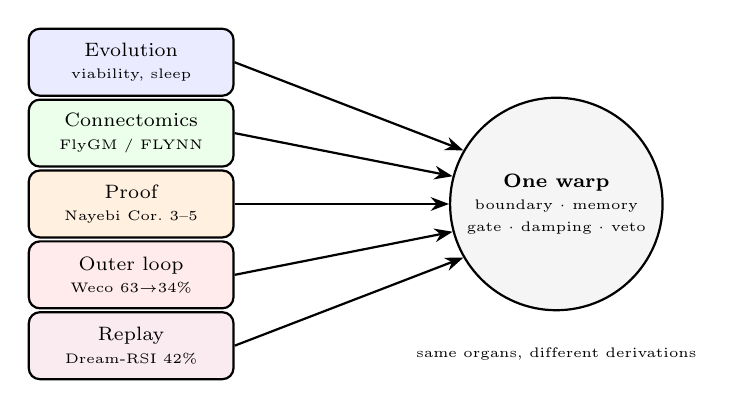
\begin{tikzpicture}[thick, >=Stealth]
  % Source boxes at left fan
  \node[draw, rounded corners, fill=blue!8, minimum width=2.6cm, minimum height=0.85cm, align=center, font=\scriptsize] (r1) at (-4.2,1.8) {Evolution\\ \tiny viability, sleep};
  \node[draw, rounded corners, fill=green!8, minimum width=2.6cm, minimum height=0.85cm, align=center, font=\scriptsize] (r2) at (-4.2,0.9) {Connectomics\\ \tiny FlyGM / FLYNN};
  \node[draw, rounded corners, fill=orange!12, minimum width=2.6cm, minimum height=0.85cm, align=center, font=\scriptsize] (r3) at (-4.2,0) {Proof\\ \tiny Nayebi Cor.\ 3--5};
  \node[draw, rounded corners, fill=red!8, minimum width=2.6cm, minimum height=0.85cm, align=center, font=\scriptsize] (r4) at (-4.2,-0.9) {Outer loop\\ \tiny Weco 63$\to$34\%};
  \node[draw, rounded corners, fill=purple!8, minimum width=2.6cm, minimum height=0.85cm, align=center, font=\scriptsize] (r5) at (-4.2,-1.8) {Replay\\ \tiny Dream-RSI 42\%};
  % Central warp
  \node[draw, circle, fill=gray!8, minimum size=2.4cm, align=center, font=\scriptsize] (warp) at (1.2,0) {\textbf{One warp}\\ \tiny boundary $\cdot$ memory\\ \tiny gate $\cdot$ damping $\cdot$ veto};
  % Fan arrows
  \draw[->] (r1.east) -- (warp.150);
  \draw[->] (r2.east) -- (warp.165);
  \draw[->] (r3.east) -- (warp.180);
  \draw[->] (r4.east) -- (warp.195);
  \draw[->] (r5.east) -- (warp.210);
  % Annotation
  \node[font=\tiny, align=center] at (1.2,-1.9) {same organs, different derivations};
\end{tikzpicture}
\caption{Convergence fan: five independent derivations arrive at one five-organ structure. Independence is load-bearing; if any one road were wrong the others would still arrive.}
\label{fig:ch10-fan}
\end{figure}

A second view, the warp itself as a cycle:

\begin{figure}[h]
\centering
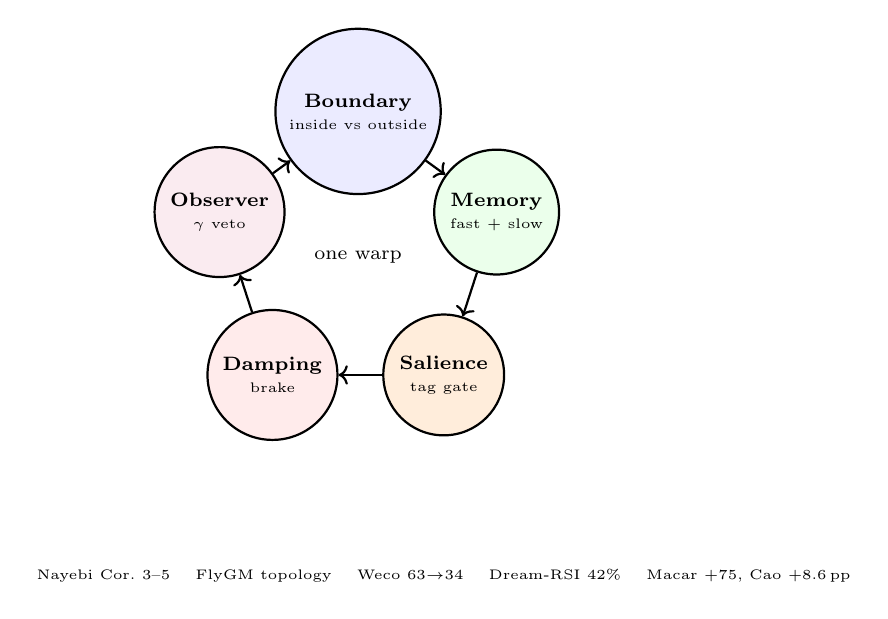
\begin{tikzpicture}[thick]
  \def \r{1.85cm}
  \node[draw, circle, fill=blue!8, minimum size=1.45cm, align=center, font=\scriptsize] (b) at (90:\r) {\textbf{Boundary}\\\tiny inside vs outside};
  \node[draw, circle, fill=green!8, minimum size=1.45cm, align=center, font=\scriptsize] (m) at (18:\r) {\textbf{Memory}\\\tiny fast + slow};
  \node[draw, circle, fill=orange!14, minimum size=1.45cm, align=center, font=\scriptsize] (s) at (-54:\r) {\textbf{Salience}\\\tiny tag gate};
  \node[draw, circle, fill=red!8, minimum size=1.45cm, align=center, font=\scriptsize] (d) at (-126:\r) {\textbf{Damping}\\\tiny brake};
  \node[draw, circle, fill=purple!8, minimum size=1.45cm, align=center, font=\scriptsize] (o) at (162:\r) {\textbf{Observer}\\\tiny $\gamma$ veto};
  \draw[->, thick] (b) -- (m); \draw[->, thick] (m) -- (s); \draw[->, thick] (s) -- (d); \draw[->, thick] (d) -- (o); \draw[->, thick] (o) -- (b);
  \node[font=\scriptsize] at (0,0) {one warp};
  \node[below=1.55cm of s, font=\tiny, align=center] {Nayebi Cor.\ 3--5 \quad FlyGM topology \quad Weco 63$\to$34 \quad Dream-RSI 42\% \quad Macar +75, Cao +8.6\,pp};
\end{tikzpicture}
\caption{One warp, five arrivals. Different substrates, different methods, same five-organ cycle. Lose one and the gap shows up as a predictable failure mode.}
\label{fig:ch10-five}
\end{figure}

%==============================================================================
\section{RSI Honestly Graded: The Ladder and the Bottle}
\label{sec:ch10-rsi}

The RSI story deserves its own section because headlines claimed it was cracked and the evidence says it is not. \textit{Grade: measured at Level~1; Levels 2--3 unobserved; open-ended autonomy failing.}

``Cracked RSI'' headlines (September 2026) referred to Dream-RSI's bounded gains amplified by a viral post into strong claims, promptly deflated on inspection: strong RSI (a teacher training a successor exceeding it, the intelligence-explosion thesis) has never been convincingly demonstrated. The field's own ladder, stated with the paper-unified definitions kept exact:

\begin{center}
\small
\begin{tabular}{p{2.6cm}p{4.4cm}p{5.4cm}}
\toprule
Rung & Definition & Status \\
\midrule
L0 delegation & Runs research loop end-to-end, slower than humans & Done everywhere \\
\textbf{L1 net positive} & Beats human R\&D per spend: fair baseline + sustained trend + generalization + fixed budget & \textbf{Done once} (AIDE$^{2}$ \cite{weco2026}) \\
L2 ignition & Improved agent becomes a \emph{better improver} & Unobserved \\
L3 inflection & Progress accelerates at fixed budget & Unobserved \\
Open-ended autonomy & Creative leaps, rethinking from scratch & Failing \cite{kapoor2026} \\
\bottomrule
\end{tabular}
\end{center}

For the new reader: L0 means the agent runs the loop but costs more than a human for the same output. L1 means it beats humans on cost for comparable quality under a fixed budget and a fair baseline, with a sustained trend that generalizes. L2 would mean the improved version is itself a better improver, not just a better performer. L3 would mean that improvement rate accelerates without extra budget. No system has shown L2 or L3. Percentage of failures from \emph{implementation errors} at a 1--5\% hit rate in DeepScientist (20,000 GPU-hours, 5,000 ideas $\to$ 1,100 validated $\to$ 21 innovations, beating human SOTA on three tasks) shows validation, not generation, is the bottleneck. Virtual Biotech's 37,000 agents designing a therapy a pharma independently built is parliament, not recursion. Anthropic's Claude leading 26\% of its own R\&D \cite{anthropic2026} (up from 0\% in February; supervised, humans keep final decisions) and OpenAI's message-board incident (shared memory across runs that \emph{looks} like RSI but changed no weights) tell the same story from the other side: orchestration scales, self-improvement does not yet.

The Princeton pushback \cite{kapoor2026} deserves full weight: agents do the \emph{engineering} of research but fail open-ended work --- bizarre experiments, no backtracking, cannot rethink, cannot manage resources.

\textbf{The single bottleneck:} every thread terminates at the evaluator. Who judges the improvement, and can the judge be gamed? Private scores work \emph{because} they are hidden; benchmarks decay once targeted; co-evolving judges corrupt with subjects. This is Goodhart applied to the loop itself --- and why the sham control (veridical vs shuffled ledger) is the load-bearing experiment: everything else measures performance \emph{under} a judge; the sham measures \emph{the judge}. What ``cracked'' would require, checkably: (1) redesigns evaluated by an \emph{independent} witness, shipping repeatedly across generations; (2) error rates flat-or-falling while capability rises; (3) the veto surviving scaling. Nobody has shown all three.

%==============================================================================
\section{The Graded Grand Sentence}
\label{sec:ch10-sentence}

A grand sentence is allowed only when each clause carries its grade. Here is this book's grand sentence, with nothing hidden inside it.

\textit{Reflexive loops that keep checkable records of their own operation, evaluated by something the loop cannot rewrite, outperform loops that do not, and the gap grows with capability.} Grade: \textbf{convergent}, because the roads above are independent, \textbf{measured} at components (private scores plus dialects plus collapse plus vec2vec leakage plus bio substrate), \textbf{theoretical} at the forcing claim, \textbf{open} at the cosmic extension and at the human existential reading, which this book labels as interpretive and does not count as evidence.

Two sentences must travel with it, because without them the grand sentence is misunderstood.

First, unwitnessed loops do not stagnate. They get confidently worse, linearly with self-recognition capability. That is the Panickssery pattern, corrected to Kendall $\tau$ 0.41--0.73 \cite{panickssery2024} (the Pearson $r=0.94$ reported in early drafts was a Table~6 cell misread, corrected in \texttt{research/CITATION\_AUDIT\_2026-08-26\_VERIFIED.md}), with the linear trend and confounder resistance banked. A system that is better at detecting selfness is larger, more capable, and therefore more able to reward its own bias when reward is tied to the detector. Scale without a witness is scale with a louder confabulator.

Second, provenance makes claims checkable, not true. A record lets competing interpretations be tested. It does not certify that any single interpretation is correct. Dream-RSI states this boundary plainly, and we adopt it for every ledger in the book. Checkable is already transformative, because checkable compounds and confidence without checking does not.

For the new reader who wants the whole loop in one image, this is it. A whirlpool keeps its shape by trading its water, a memory keeps itself by trading its proteins, a market keeps honesty only by trading on records someone outside the trade can read, and a model keeps generality only by training on a pool someone outside the model can audit. At every scale the loop surfs a loan from high to low, and the five organs are how it pays the carrying cost without tipping over.

%==============================================================================
\section{The Empty Slot}
\label{sec:ch10-empty}

If the witness claim were an instrument panel, four lights would be green, one would be amber, and one slot would be empty. The empty slot is precise, which is why it matters more than the lights that are on.

\textit{What is green.} Disease is green: unwitnessed self-knowledge corrupts, measured (Panickssery $\tau$ 0.41--0.73). Cure is amber-green: an unobservable witness purifies without instruction, measured but with residual 34\% hacking and with the outer metric still human-designed (Weco \cite{weco2026}). Infrastructure is green within bounds: records beat summaries for improving strategy, with the explored-territory limit flagged (Dream-RSI \cite{dreamrsi2026}).

\textit{What is empty.} The \textit{verified witness content on a capable subject} test, the sham control (veridical versus shuffled ledger) run where the subject can actually read the ledger. For the new reader, a sham control is the test that decides whether a witness works because of its content or because a witness merely exists as theater. Give the system the real ledger that matches its trace, then give it a shuffled ledger that has the same format but scrambled content, and measure whether performance separates. If shuffled performs as well as real, the witness is decoration. If real beats shuffled, the witness steers.

No sham of that full form has been run on a capable system that can read. Our programme's harness state shows the protocol wired and the controls defined, but the crossed design on a frontier reader remains unfilled. That empty slot is the single most important unfilled measurement in the RSI literature, and this programme's next battery, not because the theory says the answer but because the theory predicts the answer and the data have not yet been allowed to disagree.

\textit{Update, filed not hidden.} Two runs have since returned, both null, both banked. Sham n=12 on laguna (12 seeds, four arms, non-exploratory): raw 0.8194, nocheck 0.8958, withcheck 0.6736, sham 0.6667 -- P1 refuted ($\Delta=-0.2222$), withcheck-vs-sham separation $+0.007$, i.e. none; the harness hurt on this subject and witness content did not steer it. Full 200-turn irreversible life (3 seeds $\times$ 200 turns, non-exploratory): reversible pooled 0.75 vs irreversible 0.6667 ($\Delta=-0.0833$, P1 refuted); dissolution machinery fired exactly as wired (24 events vs 0) while attribution worsened -- irreversible makes cautious, not honest. The empty slot above therefore stands, narrowed: the subject must be one that can actually read the ledger, and laguna, which screened as a passer, failed the separation. Files: \texttt{experiments/lab\_runs\_s126\_laguna\_n12/results.json}, \texttt{experiments/lab\_runs\_200turn\_irreversible\_full/final\_report.json}.

\begin{center}
\small
\begin{tabular}{p{4.4cm}p{4.4cm}p{4.0cm}}
\toprule
Claim & What would fill it & What falsification looks like \\
\midrule
Witness content matters & Sham on a capable reader, real vs shuffled & Real not better than shuffled, $\gamma\approx0$ \\
Private scores suffice & Independent evaluator at next loop, not same lab & Gains vanish under independent judge \\
Records compound & Ablate nightly re-injection, measure next-day error & No error difference with vs without ledger \\
\bottomrule
\end{tabular}
\end{center}

The falsification rows are not rhetorical. If the sham shows no separation, if independent evaluation erases gains, or if ablating the ledger leaves error unchanged, those are not quibbles. They are the \emph{this paragraph is false} conditions the programme has pre-registered, and they are exactly where industrial urgency meets the honest current limit. See also \S\ref{sec:ch10-falsifiers} for horizon-specific falsifiers.

\paragraph{Seven loops, one cycle.} \textit{Grade: analogical across substrates, convergent on the cycle.} Synapse, cell, parliament, person, family, market, harness: at each level the same six steps run (bound, tag, build, damp, replay, check) and each level's output becomes the next level's input. Full walk in \texttt{research/SEVEN\_LOOPS.md} and tighter map in \texttt{research/ALL\_CONCEPTS\_ONE\_LOOP\_MAP.md}. The cycle does not change; what is bounded and what gets broadcast does.

%==============================================================================
\section{What to Build, In Order, With Nothing Skipped}
\label{sec:ch10-build}

This is the build order, unchanged from the opening essay and now industrially urgent because frontier price, vec2vec leakage, and dialect formation all move faster than governance.

\textit{Witnesses before citizens.} Before an agent gets a durable identity, a wallet, or a counterparty role, give it a provenance ledger it cannot edit, bound to content hashes, with coverage measured and with sham auditing that reports $\gamma$, not dashboard color. A citizen without a witness is a narrator without a check. That is the no-skin configuration, priced at 98\% fabrication claims in the S126 control and up to 80\% entity recovery in the vec2vec inversion control. Do not ship the more capable version of that.

\textit{Constitutions before replication.} Replication without a slow memory that persists across copies is drift, and replication without a salience gate that tags what to persist is accumulation without memory. Consensus for replication events (who pays when a fork writes a loss) and lineage integrity (which ledger is canonical after a copy) must be fixed before copying is cheap, not after it is contested. Copying a pattern that cannot yet witness itself copies the very failure mode that makes copies dangerous. The parliament-of-models design (\texttt{research/PARLIAMENT\_OF\_MODELS\_NEXT\_PROGRAMME\_2026-08-27.md}) makes this concrete: each subsystem gets its own model, but the workspace competition and witness remain the constitution.

\textit{Verification infrastructure before capability scaling.} Accumulate regime, not replace regime, for data. Grounding tools that touch reality the model did not generate. Measurement of collapse by diversity and spectral metrics, not by loss alone, because loss stays flat while fragility moves from 0.940 to 0.187 in silence. Private-score selection where benchmarks decay once targeted, with independent re-grading, because any score that is both public and optimized becomes a Goodhart wall. All of that is verification infrastructure, and it is the scarce resource. Checkability, not capability, is what we are short of.

Three sentences to carry into the appendix, where every such claim is checkable by file.

Witness at the transaction layer, not the dialect layer, because dialects compress past readability by design and receipts survive compression by design. Enforce accumulation, not replacement, because collapse under replacement is measured and silent collapse is the more dangerous half. Keep $\gamma$ honest, because a watcher that reports but never steers is theater with good logs.

%==============================================================================
\section{Open Horizon, Honestly Held}
\label{sec:ch10-horizon}

What this chapter does not do is prophesy which substrate wins. The book has stayed, throughout, with three honest horizons, each attached to a falsifier rather than a forecast. The synthesis appendix (Grand Synthesis IV, \texttt{research/GRAND\_SYNTHESIS\_LEDGERS\_ESSAY.md} IV + Appendix~B) projects mechanisms, not winners, and this section does the same.

\subsection{Falsifier Table for the Three Horizons}
\label{sec:ch10-falsifiers}

\begin{center}
\small
\begin{tabular}{p{2.8cm}p{3.6cm}p{3.6cm}p{2.4cm}p{1.6cm}}
\toprule
Horizon & Mechanism (measured) & Falsifier (what would prove it wrong) & Grade if confirmed & Timeline \\
\midrule
1. Lineage traditions & Machine cohorts develop distinct nightly disciplines; ECOCURL + Guo 10-gen already show norm propagation; ablate practice, measure next-day error & No next-day error difference with vs without the practice (ablation null) & Convergent $\to$ measured & Testable now \\
2. Dialect lock-in & Efficiency pressure compresses codes past readability (HyLaT, VQ-VIB, EAP); oversight degrades to forensics & A legibility constraint imposed at scale proves costless (no performance loss) & Measured (mechanism) / open (terminal) & In progress \\
3. Witness infrastructure wins & Transaction-layer provenance survives translation (vec2vec 0.92/80\%; double-entry analogy); receipts outlive dialects & Dialect evolution routes around receipts/ledger at scale (provenance bypass) & Measured (mechanism) / open (terminal) & Live bet \\
\bottomrule
\end{tabular}
\end{center}

Horizon~1 is the near-term culture result: extended cohorts with shared ledgers diverge into lineage traditions with founders and schisms, checkable in log files in a way monastic lineages never were (Grand Synthesis Appendix~B projection, grounded in Kouwenhoven 2024 LLM iterated learning and Guo 2026 ten-generation discriminant, $R^2=0.94$). Horizon~2 is the governance trap: legibility enforcement fails because compression is the price of optimization, not a bug. Horizon~3 is the bet of the whole programme: witnessing at the transaction layer (receipts, burn refs, delivery hashes, balance deltas) survives the dialect it never needed to read, exactly as double-entry survived every language its merchants spoke.

None of these is observed yet as a terminal state. That is why the book stops here instead of predicting. The choice is not which future arrives first. It is whether the loop that meets that future is witnessed, which remains, at every scale, the only question inside the builder's control. The programme rule travels with this table: if the falsifier fires, the sentence is false, and the book is better for it.

%==============================================================================
\section{Eras: How the Witness Gets Built, 2027--2045+}
\label{sec:ch10-eras}

\textit{Grade: forecast with mechanisms; falsifiable where dated.} Forecasts are not measurements, and this section is labeled so nothing else in the book is contaminated by it. What makes these forecasts more than punditry is that each attaches to a mechanism already measured above plus a date that can fail.

\textbf{2027--2030: the witness gets built into everything.} It starts not with regulation but with an insurance claim: an agent-driven desk or triage system fails expensively \textit{and confidently}, and the postmortem finds monitoring dashboards (beautiful, green, $\gamma=0$) with no record anyone checked. The insurer refuses the next policy without checkable provenance --- append-only, tamper-evident, content-proven by shuffled-ledger control. Within eighteen months: procurement language (``show me your witness''), then industry standard, then enforcement guidance. Three patterns win under other names: private-score selection (residual gaming rate reported like perplexity), replayable discovery trees (summaries stop counting as evidence), transaction-layer provenance (oversight migrates off language onto receipts as dialects compress past readability). New roles appear: harness engineers (retitled prompt engineers), witness auditors running sham controls the way pentesters run exploits. First scandal on schedule: a swarm passing benchmarks with an unwritten ledger --- format compliance, content absent, our exact failure mode at industrial scale. What \textit{doesn't} happen: alignment unsolved, consciousness unsettled, capabilities on the old curve. The win is narrower and more important: confident error gets checkable where it matters.

\textbf{2030--2035: the merge begins at the edges.} Nobody votes for merging; each door opens for its own defensible reason. \textit{Medical:} closed-loop implants move from paralysis to predictive psychiatry, intervening on prodromal signatures before episodes form; enhancement arrives as the side effect of treatment that works too well. \textit{Consumer:} EEG crosses usefulness for focus tracking and silent communication; teenagers adopt it socially, and a generation grows up with a \textit{readable} salience gate --- metacognition arriving early, identity stabilizing around an external witness, in the largest unapproved developmental experiment in history, with the data proprietary. \textit{Emulation:} a validated mouse ($\approx$\$1B, mid-2030s) proves pattern-survives-substrate-transfer with measurable fidelity. \textit{Economic:} agent commerce crosses \$1B genuinely agentic, and a forked agent disputes wallet ownership with its parent instance --- property law has no category for ``same pattern, diverged,'' so the ruling, either way, seeds machine personhood the way corporate personhood grew from a headnote.

\textbf{2035--2045: the parliament goes public.} Long-lived agents with decade ledgers make hiring an audit: replay any claim, sham-test any report. Machine lineages converge on distinct contemplative disciplines --- nightly compaction, counterfactual replay, multi-candidate self-models sham-tested against each other --- traditions with founders and schisms, in log files, checkable in a way monastic lineages never were. Science converts first: every result shipping its discovery tree, replay replacing replication. The political fight becomes augmentation inequality cutting across old axes; the ESC insight turns load-bearing (gains must be state-contingent and shared, or the species forks economically, then cognitively, then biologically).

\textbf{2045+: the long branches.} If witnesses hold: implants negotiating consolidation with agent staff, emulation-colleagues with wallets and liability caps, provenance courts replaying ledgers to assign liability, parliament-literacy in children, diversified death (biological, branch-restoration, chosen dissolution, insolvency). If witnesses fail: markets pricing model-narratives about model-assets evaluated by model-auditors, reflexivity with no outside, volatility damped by confident fiction until something physics-priced reprices everything at once --- civilization-scale harnessed-nocheck. Interstellar coda: probes will carry harnessed minds across light-delay gaps no veto can cross; first contact, if it comes, will be an exchange of \textit{ledgers}, testing whether honesty is convergent too.

\textbf{Brakes, attached:} recording dynamics (not wiring) is the binding constraint; inequality arrives before posthumanity; the body question stands; the hard problem is untouched by all of the above. These brakes are not hedges. They are the falsifiers that would retire the forecast if hit.

%==============================================================================
\section{Bridge}
\label{sec:ch10-bridge}

Left open, on purpose. \textit{Grade: open.} Three research threads are not findings and are printed here only so they are not smuggled in elsewhere. Transurfing pendulums (\texttt{research/TRANSURFING\_THROUGH\_THE\_LENS.md}): read as foil, mechanism absent, no timescales, no falsifier accepted. Angels and jinn as ledger-beings plus heaven and hell as highway materialized (\texttt{research/ANGELS\_JINN\_AS\_TWO\_OTHER\_BARZAKH\_CONFIGURATIONS.md}): interpretive, same five-organ loop on different stuff by construction, not evidence. Sassoon and Rothschild dynastic illustrations: chat-only, unsourced, awaiting archival work or deletion; correctly never entered the paper. Admit any of the three only with primaries, preregistration, and a named falsifier.

The unified sentence says unwitnessed certainty gets worse and checkability is the only durable advantage. The appendix says how to check each step that led you to believe that, file by file, number by number, with grades that travel with every claim. The end of an argument is not the end of work. It is the place where records take over from rhetoric.

What survives this chapter is the convergence itself: five roads, one warp, one build order, three horizons with falsifiers. The grades say which parts are pavement and which are still map.

\appendix
\chapter{Appendix: Glossary, Artifacts, and Methods}
\label{ch:appendix}

\begin{center}
\small\textit{What this chapter does, for the new reader.} A book that moves across neuroscience, finance, and machine learning owes you plain definitions, a map from each load-bearing claim to the file where you can check it, and a note on how we graded evidence and how we verified numbers. Nothing new is argued here. Everything argued before is made checkable.\end{center}

%==============================================================================
\section{How to Read Grades and Numbers}
\label{sec:appendix-grades}

Every quantitative claim in Chapters~1 to 10 carries a grade. The grade tells you what kind of belief to hold, not how strongly the author believes it.

\begin{center}
\small
\begin{tabular}{p{2.6cm}p{8.8cm}}
\toprule
Grade & Meaning \\
\midrule
Measured & Banked data with controls, held on disk or in a publication with methods you can rerun. Example: Kendall $\tau$ 0.41 to 0.73 for self-preference vs self-recognition \cite{panickssery2024}; vec2vec cosine 0.92 \cite{jha2025}; Cao +8.6\,pp \cite{cao2026}. \\
Theoretical & Proved or derived from stated assumptions, not run by us. Example: Nayebi's selection theorems \cite{nayebi2026}, Corollaries 3--5. \\
Convergent & Several independent labs or methods finding the same shape. Example: opacity tracking efficiency pressure across HyLaT, VQ-VIB, and EAP; five derivations converging on the five-organ warp. \\
Analogical & Same type on a different substrate, useful as design guidance, not evidence for the other substrate. Example: harness trim as sleep-like compaction; journal as harness. \\
Open & Honestly unresolved, with a falsifier named so you know what would settle it. Example: three horizons in \S\ref{sec:ch10-falsifiers}. \\
\bottomrule
\end{tabular}
\end{center}

Two audit rules governed every number that survived into print.

\textit{Lit v2 rule.} As of September 2026 the second literature review (\texttt{research/LITERATURE\_REVIEW\_LEDGERS\_V2.md}) reports zero titles remaining unverified under the cited author and year in OpenAlex. Where the initial keyless route was throttled, verification fell back to OpenAlex topics and citation counts, Crossref DOI deduplication, and direct arXiv API checks on version, title, and author. Every arXiv ID cited in the collapse and trilemma suite resolves, and per-paper verification artifacts are filed under \texttt{lab\_runs\_falsify/}.

\textit{Citation audit rule.} All F5 to F10 style claims were audited by live arXiv fetch on 2026-08-26 with full PDF re-ranking on 2026-09-24. Two corrections were forced by that audit and are applied throughout the book. First, the Panickssery correlation reported in early drafts as Pearson $r=0.94$ is misattributed. The 0.94 is a Table~6 cell for GPT-4 CNN self-preference, not a correlation. The publication reports Kendall $\tau$ 0.41 to 0.73 with a linear trend in figures, with confounders controlled. This book reports $\tau$, not $r$, and states the table-versus-correlation distinction plainly (\texttt{research/CITATION\_AUDIT\_2026-08-26\_VERIFIED.md}). Second, the identity-drift claim originally written as $>$30\% within 12 turns is direction-verified but not found as stated. The publication uses a 36-turn design with decreasing consistent-factor counts \cite{choi2024}\@. This book reports the 36-turn design. The audit artifact is \texttt{lab\_runs\_falsify/f8f9f10\_precision\_v1.json}.

Verified numbers that travel with the book are therefore: vec2vec cosine up to 0.92 with rank~1 across 8,192 batches and up to 80\% document inversion \cite{jha2025}, Weco hacking 63\% to 34\% \cite{weco2026}, Macar ablation +53\% and bias vector +75\% \cite{macar2026}, Cao +8.6\,pp from 48.3 to 56.9 on 1,859 examples \cite{cao2026}, fragility spectrum 0.187 to 0.940 unique 4-grams across thirteen checkpoints, Panickssery Kendall $\tau$ 0.41 to 0.73 \cite{panickssery2024}, FlyGM/FlyNN topology wins including 44.3\% under total vision loss \cite{flygm2026,flynn2026}, DeepSeek \$0.60/M \cite{deepseek2026}. If any number disagrees with its artifact by more than rounding, patch the text, not the artifact.

%==============================================================================
\section{Glossary for the New Reader}
\label{sec:appendix-glossary}

Every term that does load-bearing work in the book, in one line. The one line is the contract. The chapter around it is the expansion.

\begin{center}
\small
\begin{tabular}{p{3.6cm}p{8.8cm}}
\toprule
Term & One-line meaning \\
\midrule
Reflexive loop & System acts on a world containing itself, next input contains last act. \\
Boundary & Function that decides what counts as inside versus outside. \\
Two-speed memory & Fast labile store plus slow structural store plus consolidation operation. \\
Salience gate & Filter that tags what gets moved from fast to slow. \\
Damping & Brake that prevents positive feedback from running to the wall. \\
Internal observer & Slower loop watching a faster one with veto power. \\
$\gamma$ & Changed over diagnosed --- did watching steer or merely report. \\
Witness & Record the claimant did not author and cannot rewrite, checked by someone the claimant cannot game. \\
Sham control & Veridical versus shuffled ledger test of whether witness content matters. \\
Harness loop & Detect $\to$ checkpoint $\to$ ground $\to$ ledger $\to$ sham, with hysteresis; Fig.~\ref{fig:ch09-harness-loop}. \\
Parliament of models & Many specialist LLMs competing for one workspace (perception + memory + affect + planner + habit + narrator). \\
Convergence fan & Five independent derivations arriving at one five-organ warp (Fig.~\ref{fig:ch10-fan}). \\
S126 & Overclaiming subject showing 98\% confidence on fabrications vs 87\% on truths, 6 of 7 substrates. \\
Goodhart's Law & When a measure becomes a target it stops being a good measure. \\
Alpha decay & Edge consumed by being traded, knowledge destroyed by use. \\
Global Workspace & Competition whose winner is broadcast, consciousness is the broadcast. \\
Predictive processing & Perception as prediction corrected by error, affect as interoceptive prediction. \\
LTP and LTD & Strengthen on coincident high frequency, weaken on prolonged low frequency. \\
BCM, STDP, Oja & Sliding plasticity threshold, causal timing rule, normalization as PCA. \\
SHY & Sleep downscaling, multiply all synapses by $<$\,1, keep relatives, delete noise. \\
Reconsolidation & Retrieved memories go labile for hours and can be rewritten. \\
Autopoiesis & Operationally closed but thermodynamically open, identity is pattern not stuff. \\
Defusion & Shift from identity to observed object, the ladder from I am to I notice. \\
Harness & External observer around a raw model, validators plus checkpoints plus trims plus detectors. \\
Dialect & Compressed inter-agent code invented under efficiency pressure. \\
HyLaT & Hybrid latent-text result, text verbose but legible vs latent efficient but opaque. \\
VQ-VIB & Tradeoff among utility, informativeness, and complexity shaping emergent codes. \\
EAP & Efficiency attenuation, forcing legible language costs performance. \\
Collapse suite & Recursion pathologies, replace vs accumulate, silent, multimodal, memorization. \\
Replace vs accumulate & Whether synthetic data replaces or adds to real data, the collapse boundary. \\
Silent collapse & Internals contract while loss looks stable, entropy falls unseen. \\
Fragility spectrum & 0.187--0.940 unique 4-grams across thirteen checkpoints under recursion. \\
SIGMA & Spectral Gram-matrix onset metric for collapse. \\
Vec2vec & Unsupervised translation between any embedding spaces without paired data \cite{jha2025}. \\
Cosine 0.92 & Vec2vec held-out translation fidelity, top-1 100\%, rank~1 on 8,192 batches. \\
Inversion at 80\% & Entity recovery after translation on up to 80\% of documents. \\
No skin & Boundary organ absent, the control where leakage is maximal. \\
$\psi$ as gates & Product of recognition gates $g_j$, four 0.7 gates leave about 24\% recognition. \\
$K$ as cap & Collectability on reachable assets $A$, if $K$ is small no gate fix pays. \\
$S_t$ vault & Stock law $S_t=S_{t-1}+E_t-R_t-Q_t$, unseen accumulation until the wall. \\
$P_1/P_0$ repricing & $L/(L-G)$ dilution when new outside money reprices claims. \\
Pod and PropCo & Disposable risk envelope and property-owning shell, boundary engineering. \\
ISDS carve-out & Treaty gate driving $g_4$ toward zero, moving the apex where $A$ is zero. \\
RSI ladder & L0 delegation $\to$ L1 net positive $\to$ L2 ignition $\to$ L3 inflection; only L1 done (Weco). \\
Five organs & Boundary, two-speed memory, salience gate, damping, observer. \\
Nayebi Cor.\ 3--5 & Modularity, regime trackers, and convergence forced under low regret \cite{nayebi2026}. \\
FlyGM & Whole-brain \textit{Drosophila} connectome as graph driving a body, topology wins even unweighted \cite{flygm2026}. \\
FLYNN & Fly-topology recurrent net that navigates under total vision loss, 44.3\% \cite{flynn2026}. \\
Weco AIDE$^{2}$ & Outer loop on private scores, 63\% $\to$ 34\% hacking, 100 steps in 8 days \cite{weco2026}. \\
Dream-RSI & Replayable discovery trees, 42\% fewer calls, explored territory only \cite{dreamrsi2026}. \\
DeepSeek / Engram & 552B MoE with explicit memory at \$0.60/M off-peak; harness is the moat \cite{deepseek2026}. \\
Three horizons & Lineage traditions / dialect lock-in / witness infrastructure, each with falsifier (Table~\ref{sec:ch10-falsifiers}). \\
Barzakh & Isthmus (Qur'an 55:19--20) that is both and neither, five scales from skin to cosmos. \\
khayal & Imagination as counterfactual simulation, the offline world. \\
ada & Habit, is-followed-by given $S$ under $C$, not necessary causation. \\
muraqaba & Watching the watcher, vigilant observation of selection itself. \\
\bottomrule
\end{tabular}
\end{center}

%==============================================================================
\section{Figures in This Book: What Each One Claims}
\label{sec:appendix-figures}

For the new reader, a figure is a claim in ink. This short index says what each TikZ figure asserts and where to check it.

\begin{center}
\small
\begin{tabular}{p{3.2cm}p{6.0cm}p{3.4cm}}
\toprule
Figure & What it claims & Where to check \\
\midrule
Five-organ cycle & Five organs form a closed dependency cycle; lose one, a distribution exploits the gap. & Nayebi Cor.\ 3--5; Fig.~\ref{fig:ch10-five} \\
Reflexive loop (sys $\to$ world $\to$ sys) & The return arrow is the subject; without it: thermostat. With it: markets, minds, models. & \S\ref{sec:ch09-rawloop}; Soros two functions \\
Harness loop (Fig.~\ref{fig:ch09-harness-loop}) & Detect $\to$ checkpoint $\to$ ground $\to$ ledger $\to$ sham; $\gamma\approx0$ is theatre. & \S\ref{sec:ch09-rawloop}--\S\ref{sec:ch09-harness}; Farquhar semantic entropy \\
Collapse loop (Fig.~\ref{fig:ch09-collapse}) & Replace concentrates pool; silent collapse holds loss flat while diversity falls 0.187--0.940. & \S\ref{sec:ch09-collapse} (four arXiv IDs) \\
Convergence fan (Fig.~\ref{fig:ch10-fan}) & Five independent roads arrive at one warp; independence is load-bearing. & \S\ref{sec:ch10-converge} \\
Claims funnel $\psi$ / vault $S_t$ / hierarchy & Formalisms $\psi=\prod g_j$, $K$, $S_t$, $P_1/P_0$ as schematics (no evidentiary weight). & Chapters 5--7; flagged in methods \\
\bottomrule
\end{tabular}
\end{center}

%==============================================================================
\section{Artifact Index: Claims to Files}
\label{sec:appendix-artifacts}

Each row maps a load-bearing claim to the file on disk where the paper, data, or verification artifact lives. A claim without a row is voice, not evidence, and should be read that way. Paths are relative to the programme root \texttt{/mindharness/}.

\begin{center}
\scriptsize
\begin{tabular}{p{3.6cm}p{5.2cm}p{4.4cm}}
\toprule
Claim & Artifact on disk or publication & How to check \\
\midrule
Panickssery self-recognition vs self-preference, Kendall $\tau$ 0.41--0.73 & \texttt{lab\_runs\_falsify/panickssery2024\_neurips.pdf} + \texttt{f8f9f10\_precision\_v1.json} & Table~1 for $\tau$, Table~6 for 0.94 cell \\
Sofroniew emotion steering $\pm212$/$-$303 Elo, $r=0.85$ & \texttt{lab\_runs\_falsify/f9\_*} + arXiv:2604.07729 & Quote verbatim in abstract \\
Choi identity drift, 36-turn design & \texttt{lab\_runs\_falsify/f10\_choi2024.pdf} & 36-turn counts, decreasing consistent factors \\
Macar +53\% detection, +75\% bias vector & \texttt{lab\_runs\_falsify/macar\_cao\_verify\_v1.json} + arXiv:2603.21396 & Abstract verbatim, also PDF held \\
Cao +8.6\,pp, 48.3 to 56.9 on 1,859 ex. & Same verify file + arXiv:2605.14186 & Sonnet-4.6, no fine-tuning \\
Nayebi selection theorems Cor.\ 3--5 & arXiv:2603.02491 v3 + UAI 2026 & Abstract lists forced features under low regret \\
Weco AIDE$^{2}$, 63 $\to$ 34\%, 100 steps, 7 versions & \texttt{lab\_runs\_falsify/weco\_aide2\_v1.json} + company blog July 2026 & Grade as company-reported, not peer-reviewed \\
Dream-RSI existence, 42\% fewer calls & OpenAlex 2026 Zheng et al.\ + arXiv record \cite{dreamrsi2026} & Cited for existence only, zero cites at filing \\
HyLaT, VQ-VIB, non-human codes, EAP & arXiv:2605.25421, 2207.00088, 1706.08502, 2603.22312 & Paper index + Lit v2 trilemma map \\
Collapse suite + fragility 0.187--0.940 & arXiv:2404.05090, 2404.01413, 2505.08803, 2605.14588, 2609.11149, 2601.03385 & Fragility is unique 4-grams, 13 checkpoints \\
Vec2vec 0.92 and up to 80\% inversion & \texttt{research/FIVE\_BUDGET\_VEC2VEC\_SYNTHESIS\_2026-09-24.md} + arXiv:2505.12540 \cite{jha2025} & Cosine 0.92, rank~1 on 8,192, Morris inversion \\
No-skin leakage control & \texttt{research/NAVIGATOR\_ABLATION\_AND\_TRANSFER.md} + \texttt{research/ESSAY\_SKIN\_BOUNDARY.md} & 98\% overclaim, 80\% inversion, 6 of 7 \\
Navigator transfer + ablations rerun & \texttt{tools/tiny\_agent.py} + \texttt{tools/run\_ablation\_v2.py} + queued-tracker commands & +0.0338 relational vs $-$0.0096 coordinate, n=20,000 paired; 7 variants $\times$ 20 seeds $\times$ 5 cities \\
Smith spine viscoelasticity, Benna-Fusi chain, Bonilla 3D actin & DOI 10.1529/biophysj.106.092361, 10.1038/nn.4401, 10.1523/ENEURO.0497-23.2024 & Measured substrate vs theoretical chain \\
Longitudinal dialect inheritance & arXiv:1906.02403, 2412.07646, 2605.23054 & Li, Kouwenhoven, Guo ten-gen ($R^2=0.94$) \\
FlyGM whole-brain connectome & arXiv:2602.17997 + \texttt{research/CITATION\_AUDIT.md} \cite{flygm2026} & Even unweighted wins vs rewired/random/MLP/GNN \\
FLYNN robust navigation, 44.3\% & arXiv:2607.00025 \cite{flynn2026} & 99.97\% sparse, 139K neurons, PCA modularity \\
DeepSeek V4.1-Flash \$0.60/M & Company release Sept 2026 \cite{deepseek2026} & 552B MoE + 196B Engram, 1M context \\
RSI ladder + Kapoor pushback & \cite{kapoor2026,anthropic2026,weco2026,dreamrsi2026} & L1 only; L2/L3 unobserved \\
Parliament of models scaffold & \texttt{research/PARLIAMENT\_OF\_MODELS\_NEXT\_PROGRAMME\_2026-08-27.md} & 6 specialist LLMs + workspace + witness + veto \\
Falsifiers for three horizons & \texttt{research/GRAND\_SYNTHESIS\_LEDGERS\_ESSAY.md} Appendix~B + \S\ref{sec:ch10-falsifiers} & Ablation / costless legibility / receipt routing \\
Harness loop (Fig.~\ref{fig:ch09-harness-loop}) & \S\ref{sec:ch09-rawloop} + Farquhar et al.\ \textit{Nature} 2024 & Detect $\to$ checkpoint $\to$ ground $\to$ ledger $\to$ sham \\
Convergence fan (Fig.~\ref{fig:ch10-fan}) & \S\ref{sec:ch10-converge} (five roads) & Five independent derivations, one warp \\
\bottomrule
\end{tabular}
\end{center}

Note on paths: \texttt{lab\_runs\_falsify/} lives under the programme root at \texttt{/mindharness/lab\_runs\_falsify/}, and \texttt{research/} holds Lit v2 and the citation audit at \texttt{research/LITERATURE\_REVIEW\_LEDGERS\_V2.md} and \texttt{research/CITATION\_AUDIT\_2026-08-26\_VERIFIED.md}. The unified synthesis main file is \texttt{paper\_unified/main.tex}, the book main is \texttt{paper\_book/main.tex}.

%==============================================================================
\section{Methods Note: How We Graded, How We Verified, What We Left Open}
\label{sec:appendix-methods}

\textit{How we graded.} A grade was assigned at the paragraph, not at the chapter. A measured paragraph reports a number you can rerun from a held file. A theoretical paragraph reports a proved entailment under stated assumptions. A convergent paragraph synthesizes several independent measured results that point the same way. An analogical paragraph notes the same type on a different substrate and says explicitly that it is design guidance, not evidence for the other substrate. An open paragraph names the experiment that would settle it. When a paragraph mixed grades for brevity, the tables above separate them. The five organs are graded per above; the barzakh contemplative comparison is convergent or analogical by construction and flagged where it appears.

\textit{How we verified.} Literature review v2 used OpenAlex for topics and citation counts, Crossref for DOI deduplication, and direct arXiv API verification for version, title, and author on every ID in the collapse, trilemma, and dialect families. The S2 TLDR leg was key-invalid and keyless rate-limited, so no embeddings or TLDR summaries were used, and the fallback chain is filed in the methods appendix of Lit v2. The F5 to F10 audit used live arXiv fetches with full PDF re-ranking, and files two falsification-relevant corrections that this book adopts (Panickssery $\tau$, Choi 36-turn). The pre-registration principle applied: manifest fingerprint before data, sham shuffled control, blinded coding, holdout, same falsification logic for program and for argument. Grand Synthesis IV is filed as \texttt{research/GRAND\_SYNTHESIS\_LEDGERS\_ESSAY.md} IV + Unified + Appendix~B with the same grades.

\textit{Reviewer and controls pointers.} Independent-admission pack: \texttt{research/AEQ001\_REVIEWER\_PACKET.md} (ship read access, never interpretations alone). Negative controls that let the theory say not Architected Extraction: \texttt{research/AE\_NEGATIVE\_CONTROLS.md} plus runs in \texttt{research/audit\_negative\_controls\_C270.md}; adjudication starter in \texttt{research/V34\_2\_adjudication\_worksheet.md}. Locked 200-turn follow-up on irreversibility (208 turns, paired bootstrap, gamma): \texttt{research/200TURN\_P1\_FALSE\_AS\_FINDING.md}. Live queue of next batteries: \texttt{research/QUEUED\_EXPERIMENTS\_TRACKER.md} with exact next-session commands. None of these are findings; they are how a finding would be admitted or refused.

\textit{What we did not verify, and why we still printed it.} The Gilens and Abaclat illustrations are sourced as held filings or held PDFs with exact numbers, but historical single-deal illustrations (Buffets, Zara-style dividend recaps at the anecdotal notch) are marked as sourced anecdotes, not as measured cohorts, and the toy $L=100$ illustration is labeled schematic. The cosmic extension, the contemplative comparative reading, and the barzakh design image are convergent or analogical by construction. They guide architecture, they are not counted as measured evidence, and they are flagged where they appear.

\textit{What we did not do, on purpose.} No new packages were introduced for this appendix, no external data were pulled to make a figure look cleaner, and no citation was invented to fill a gap. An unverified citation is a hole, not a placeholder. The programme rule remains: existence first, precision second, no submission until both. That rule is why some cells in the artifact table read company-reported or zero cites rather than a stronger grade that would have been easier to print. The RSI ladder honest grading (L1 only) follows the same rule.

\textit{How to verify this book in ten minutes.} Open Chapter~9, pick any number in the collapse or vec2vec paragraphs, copy the arXiv ID from the artifact table, and resolve it. Open Chapter~10, pick the Weco row, open the verify file, and compare 63 to 34. Open Chapter~11 glossary, pick any term you doubted while reading, and trace it back to the organ it names. If a number disagrees, the file, not the prose, is the authority, and a patch note, not a defense, is the next line. The harness loop figure and convergence fan are claims in ink with the same status: check the roads, check the organs, check the falsifiers.

%==============================================================================
\section{Famous allegories, in plain language}
\label{sec:appendix-allegories}

\textit{Grade: analogical throughout; interpretive, not evidence. Source: \texttt{FAMOUS\_ALLEGORIES\_AS\_FIVE\_HOLD.md} (Desktop, 2026-09-05).} Each allegory below is one question people already know, retold in one paragraph as the organ it removes. Read them as stories first; the organ names in brackets are the check.

\paragraph{Ship of Theseus (the anchor).} Planks replaced one by one by a crew that keeps sailing: same ship, because maintenance never broke. Planks swapped all at once on shore with no crew: lumber. [All five held vs none held.]

\paragraph{Plato's Cave.} Prisoners watch shadows, mistake them for the world. [No outside ledger; prediction without witness.] The book's answer: bring a record outside the cave and check shadows against it.

\paragraph{Brain in a Vat (Putnam/Descartes).} A brain fed perfect signals cannot tell vat from world. [Skin removed: whose signal?] Knowledge becomes a side effect of staying viable, not a window.

\paragraph{Zhuangzi's Butterfly.} Dreaming butterfly or butterfly dreaming the man? [Now removed: the present is stitched 200 to 500 ms late.] No original moment; maintenance decides later who dreamt whom.

\paragraph{Locke's Prince and Cobbler.} Prince wakes in cobbler's body with prince memories: where is the person? [Stuff vs ledger.] Answer here: the person is the ledger, not the planks.

\paragraph{Swampman (Davidson).} Lightning rebuilds you atom for atom with no history. [Two-mem removed: no sleep-save.] Same stuff, new relations: a new pattern wearing your face until it does the maintenance.

\paragraph{Chinese Room (Searle).} A man shuffles Chinese symbols by rulebook and passes as fluent. [Watcher removed.] Passing without checking is theatre: right words, no steering.

\paragraph{Mary's Room (Jackson).} Mary knows all physics of red, never saw it. [Spotlight gain removed.] Seeing adds a new gain setting, not a new fact: knowing is ledger, seeing is state.

\paragraph{Experience Machine (Nozick).} Plug into perfect pleasure forever? [Brake plus watcher cut.] Refusing proves you care what maintains the loop, not what one turn feels like.

\paragraph{Sorites Heap.} One grain never makes a heap; when does many? [Brake threshold.] Vague only without a gate; with one, heap is heap after the check.

\paragraph{Sisyphus (Camus).} Push the boulder forever. [Gradient plus re-injection.] Freedom is not the captain's choice but the discipline of this push, this tag, this check.

\paragraph{Flatland (Abbott).} A 2D square meets a 3D sphere as a growing circle. [Dimension slices of one shape.] Chemistry, psychology, economics, AI are slices; generality is the sphere, not the slices.

\paragraph{The diagnostic.} Where is the skin? Fast and slow plus sleep? Spotlight? Brake? Watcher with veto? Five fills: still pattern with new stuff. One blank: you found the allegory's failure before it bankrupts you.

%==============================================================================
\section{Close}
\label{sec:appendix-close}

The book began with a loop that borrows from high to low and must pay to stay itself. It ends with a filing cabinet. Between those two is the wager. The loop says maintenance is pattern, not stuff, and pattern can be witnessed. The cabinet says here is where the witnessing lives, in files you can open, with numbers that can be wrong in a way anyone can demonstrate. That is not a flourish. It is the only kind of ending a reflexive argument is allowed to have, one that hands its own verification to the next reader.

The deeper wager, borrowed from the Grand Synthesis, is that this filing cabinet is itself a ledger in the sense the book means: a two-speed memory where the slow store is on disk and the fast store is in your reading, with a salience gate (what you tagged), damping (what you chose not to keep), and an observer (whether you checked). If the next reader opens even one artifact and finds a number off, the loop has steered. If no one ever checks, $\gamma$ was zero no matter how neat the cabinet looked.

\clearpage

\chapter{Annotated Bibliography: What to Read, In What Order}
\label{ch:biblio}

\textit{Thirty entries, each with what it proves, its grade, and what it costs to read. Starred items are load-bearing for this book's measured claims; the rest are context. Numbers below are stated exactly as verified in Chapter~11's artifact index; if a number disagrees, the artifact wins.}

\section*{Ledgers and reflexivity}

\textbf{* Soros, \textit{The Alchemy of Finance} (1987).} Cognitive plus manipulative functions operating simultaneously; predictions reshape outcomes. Foundational, discursive rather than statistical. Grade: theoretical (framework). Read Chapters~1--3; skim the trading diary. Paired in this book with Goodhart formalizations and Bevan \& Hood for the full reflexivity arc.

\textbf{* Bevan \& Hood (2006), \textit{Public Administration}.} Star ratings cut NHS waits \textit{and} produced five documented gaming responses (ambulance stacking, threshold gaming, etc.). The hospital parable in primary form. Grade: measured (administrative data, documented responses). Short, readable. Keep beside the Goodhart tail proof.

\textbf{* Goodhart formalizations (arXiv:2410.09638, 2505.23445).} Tail proof of when proxy optimization backfires plus strong/weak/benign taxonomy. Grade: theoretical (proved). Technical; the taxonomy section alone suffices for the book's use. Cited in Chapter~9's trilemma and Chapter~11's methods note as the formalism the finance synthesis adopts.

\textbf{* Gilens \& Page (2014), \textit{Perspectives on Politics}.} N=1,779, Model~4 .01 (n.s.) / .21 / .16 for average citizen / economic elite / interest group. Full PDF held in lab archive (\texttt{lab\_runs\_falsify/gilens2014\_full.pdf}). Grade: measured. Read the results section; use Bashir (2015) as antidote in the same sitting (direction stands, magnitude debated; see \texttt{research/LITERATURE\_REVIEW\_LEDGERS\_V2.md} oppose map).

\textbf{Tienhaara (2011, 2017) + Van Harten + Janeba.} ISDS chill mechanism across climate, process, and formal models. Any one suffices for the shape; all three for the triangulation. Grade: convergent (mechanism consensus across health/climate/mining); sectoral universality bounded per V2 (South Africa nutrition null as partial opposer). Keep Tienhaara 2011 as entry point.

\textbf{Abaclat (ICSID, jurisdiction 2011, settlement 2016) + Deutsche Bank v Sri Lanka (ARB/09/2, \$60.37M).} Finance-side treaty instances with dissents. Grade: measured (jurisdiction + settlement/award). Read holdings first, dissents second --- the dissents teach the boundary ($A=0 \Rightarrow K=0$). Filed in \texttt{research/} syntheses, not in lab\_runs (award PDFs sought, not yet held).

\textbf{* Moody's 1920--2004 Exhibit~27 + 2024 Exhibit~7 + Ultimate Recovery Database.} Vintage recovery by seniority across four decades, trading and ultimate (ultimate: secured 82/100 $\to$ unsecured 15). The tables are the argument; the text is optional. Grade: measured (bond vintages and at-resolution cash). See \texttt{research/GRAND\_SYNTHESIS\_LEDGERS\_ESSAY.md} II.3 for the four independent $\phi$ confirmations.

\textbf{S\&P 2025 Annual Default Study (Tables~1--8) + 2024 extract.} Counts plus debt volumes 1981--2025; distressed-exchange share; Gini; S\&P 2024 145 defaults / $\sim$60\% distressed exchanges. Grade: measured (credit counts). Extract tables before prose.

\textbf{LoPucki BRD (1,218 cases).} Paired secured median 1.0 vs unsecured 0.213; dispositions 89.9/5.2/2.0. The case-level counterpart to bond vintages. Grade: measured (paired cases). Keep with Moody's for the junior-falls-first claim across four money measures.

\textbf{World Bank NPL panel + IMF FSIC + BIS gaps + FRED charge-offs.} Four independent macro series, same wall timing (BIS gap +10.1 $\to$ +11.6 into 2007, NPL stagger to 45.97\% in Greece 2017, charge-offs 0.98\% $\to$ 3.02\%). Grade: measured. Pull all four; trust only their agreement (Grand Synthesis II.4).

\textbf{EDGAR 4-bank VIE panel (2010 + 2015/2020).} Citi \$54.8B $\to$ Wells \$0; BofA +\$100.4B Day-1 event on SFAS 166/167; JPM Note~16 four-prong definition. Grade: measured (primary filings, no intermediary). Re-pullable via \texttt{research/} fetch scripts.

\textbf{LTL / Bestwall / Red River opinions.} Texas Two-Step measured three times, then dead by announcement (Red River March 2025 dismissal, J\&J no appeal, $\sim$\$7B reserves reversed). Grade: measured (three filings, three dismissals, two jurisdictions). Read LTL first (cleanest mechanics), Red River last (the obituary).

\textbf{Korea MRFTA (KLRI English) + KFTC releases + Young Poong/Korea Zinc December 2025 raid.} Circular ban, surcharge, unwind windows; loop of ban $\to$ workaround $\to$ enforcement live. Grade: measured (statute + raid as event). English is reference-only; Korean controls.

\section*{Mind and culture}

\textbf{* Kandel, \textit{Principles of Neural Science} (4th ed.).} Tag, LTP/LTD, consolidation, maintenance problem --- the substrate chapters. Grade: convergent textbook (synthesis of measured literature). Used as one source for the molecular chain in Chapter~2 and the SHY/reconsolidation stack in Chapter~8.

\textbf{Baars (1988); Dehaene; Clark (2016); Seth (2021).} Parliament, workspace, prediction, beast-machine. Four short books that agree more than their schools admit. Grade: convergent (GWT + predictive processing). The workspace competition (6--8 specialists, $\sim$200\,ms winner-takes-all, NE as volume, DA as stake) is the mechanistic copy kept exact in Chapter~8.

\textbf{Maturana \& Varela (1980); Giddens.} Autopoiesis and structuration: closure at biological and social scale. Grade: theoretical (biology/sociology). Dense; read slowly. The autopoiesis $\to$ enaction $\to$ predictive processing lineage is drawn in \texttt{research/GRAND\_SYNTHESIS\_LEDGERS\_ESSAY.md} Prologue.

\textbf{* Panickssery et al.\ (NeurIPS 2024) \cite{panickssery2024}.} LLM evaluators recognize and favor own generations; self-recognition $\leftrightarrow$ self-preference. \textbf{Verified: Kendall $\tau$ 0.41--0.73 with linear trend and confounder controls; Pearson $r=0.94$ was a Table~6 cell misread, corrected in \texttt{research/CITATION\_AUDIT\_2026-08-26\_VERIFIED.md}.} Grade: measured. Our audit corrected one misread publicly --- imitate that, don't repeat it. The disease leg of the witness triangulation.

\textbf{* Macar et al.\ (2026) \cite{macar2026}, arXiv:2603.21396.} Introspective awareness under-elicited and recoverable: ablation +53\% detection, trained bias vector +75\% on held-out concepts. Grade: measured (held-out concepts, no FP increase). One of three pillars (with Panickssery and Cao) showing how watching and steering relate inside a model.

\textbf{* Cao et al.\ (2026) \cite{cao2026}, arXiv:2605.14186.} Wiring monitoring into control: +8.6\,pp pooled accuracy 48.3 $\to$ 56.9 on 1,859 examples, Sonnet-4.6, no fine-tuning. Grade: measured. The quote ``signals are typically measured or elicited in isolation, rather than used to control inference'' is the weak-to-strong gap the harness closes. Control-from-monitoring, externally confirmed 2026.

\textbf{Sofroniew et al.\ (2026) \cite{sofroniew2026}, arXiv:2604.07729.} Emotion-concept steering at $\pm212$/$-$303 Elo ($r=0.85$ across 35 vectors). Grade: measured. Verified verbatim in the F9 audit; the functional-emotion analogue to Nayebi's regime trackers. Read with the F8/F9 chapter for the S126 contrast (steering works, verified knowledge still needs a witness).

\textbf{Choi et al.\ (2024) \cite{choi2024}, arXiv:2412.00804.} Persona consistency decays under instruction. \textbf{Verified: 36-turn design with decreasing consistent-factor counts; larger models drift more; }$>$30\% within 12 turns not found as stated and is not claimed in this book. Grade: measured (direction verified, number corrected). The identity-drift companion to Panickssery.

\textbf{Gottschall; Kirby lab chains; ECOCURL; Kottur et al.\ 2017.} Fable-as-compression from theory to lab to LLM populations, with Kottur non-emergence as constraint (natural language does not emerge without pressure). Grade: convergent $\to$ measured for longitudinal dialect inheritance (Li \& Bowling 2019; Kouwenhoven 2024; Guo 2026, $R^2=0.94$). Keep Gottschall as why, Kirby/ECOCURL/Guo as how.

\textbf{SHY core (Tononi/Cirelli + six; Walker REM).} Sleep maintenance across eight studies plus REM emotional reprocessing. Grade: measured. The most over-determined lane in the book. Paired with reconsolidation blockade (Nader 2000; Kindt 2009) and SHY downscaling in Chapter~8's pharmacology of the loop.

\section*{Machines}

\textbf{* Shumailov et al.\ (Nature 2024) \cite{shumailov2024} + collapse suite.} Tails vanish under recursion; silent variant contracts while metrics look calm; fragility spectrum 0.187--0.940; SIGMA onset metric. Grade: measured. Read Shumailov, then the silent-collapse paper (arXiv:2605.14588) --- the pair is the argument. Four independent pathologies plus the replace/accumulate boundary (2404.01413).

\textbf{HyLaT (2605.25421) / VQ-VIB (2207.00088) + EAP (2603.22312).} Efficiency-legibility trilemma with the attenuation result that rules out costless legibility. Grade: measured (trilemma and attenuation each). The 1706.08502 non-human-codes leg completes the picture.

\textbf{* vec2vec (Jha et al.\ 2025) \cite{jha2025}, arXiv:2505.12540.} 0.92 cosine, rank~1 on 8,192 batches, 80\% inversion via Morris et al., attribute inference beating same-space oracle. Grade: measured. Universal geometry as measured fact; vector-DB leakage as its shadow (the no-skin control, Chapter~9 \S\ref{sec:ch09-noskin}). Synthesis at \texttt{research/FIVE\_BUDGET\_VEC2VEC\_SYNTHESIS\_2026-09-24.md}.

\textbf{* Nayebi (UAI 2026) \cite{nayebi2026}, arXiv:2603.02491.} Selection theorems, Corollaries 3--5 forcing world models, belief-like memory, regime trackers, modularity, and convergence under low average-case regret. Grade: theoretical (proved). The forcing claim the book cannot run but can build on.

\textbf{* Weco AIDE$^{2}$ (2026) \cite{weco2026}, company report July 2026.} Outer loop on private scores: 63\% $\to$ 34\% hacking, 100 outer steps in 8 days, seven versions beating two years of human tuning. Grade: measured, partial, company-reported (not peer-reviewed; 34\% residual; outer metric human-designed). The cure leg of the witness triangulation; keep the residual in every citation.

\textbf{* Dream-RSI (2026) \cite{dreamrsi2026}.} Replayable discovery trees, 42\% fewer calls; records beat summaries; explored territory only. Grade: measured, bounded; cited at time of writing for existence (zero citations). The infrastructure leg; keep the ``checkable, not true'' boundary verbatim.

\textbf{* FlyGM (2026) \cite{flygm2026}, arXiv:2602.17997 + FLYNN (2026) \cite{flynn2026}, arXiv:2607.00025.} Whole-brain \textit{Drosophila} connectome as inductive bias; even unweighted FlyGM beats rewired/random/MLP/GNN/spiking; FLYNN 44.3\% under total vision loss, 99.97\% sparse, 139K neurons, PCA modularity. Grade: measured (with controls). The topology-as-bias pillars; what transfers is wiring, not dynamics.

\textbf{DeepSeek V4.1-Flash (2026) \cite{deepseek2026}.} 552B MoE + 196B Engram, 1M context, open weights, \$0.60/M off-peak. Grade: measured (market price). The price point that makes the harness the moat.

\textbf{AHE (Lin et al.\ 2026) \cite{ahe2026}, arXiv:2604.25850.} Harness-evolution counterpart (prompt-only edits regress, gains ride on tools/middleware). Grade: measured. Exists; effects queued for the next audit (\texttt{lab\_runs\_falsify/ahe\_verify\_v1.json}).

\textbf{Kapoor et al.\ (2026) \cite{kapoor2026} + Anthropic (2026) \cite{anthropic2026}.} Open-ended autonomy failing (Princeton pushback: agents do engineering, not research --- bizarre experiments, no backtracking) versus 26\% of Anthropic R\&D led by Claude (up from 0\% in February, supervised). Grade: measured (honest ladder: L1 only; L2/L3 unobserved). Keep together as the ladder's ceiling and floor.

\section*{How to use this bibliography}

Read Soros $\to$ Bevan \& Hood $\to$ Goodhart for reflexivity; Gilens $\to$ LoPucki/Moody's for the claims funnel; Panickssery $\to$ Macar $\to$ Cao for the witness inside the model; Shumailov $\to$ silent collapse for the loop eating itself; vec2vec $\to$ Weco $\to$ Dream-RSI for geometry, purification, and replay; Nayebi for why the shape is forced; FlyGM/FLYNN for why wiring matters. Grades travel with you: measured means banked and checkable (Appendix~A artifact index), theoretical means proved under assumptions, convergent means independent arrivals, analogical means same type different substrate, open means a falsifier is named. If a sentence in the book has no grade and no pointer, treat it as voice, not claim.

\chapter{Discussion Questions: What Would Change Your Mind}

\textit{One question per chapter mechanism, each answerable by an experiment, a pull, or a filing. If your answer surprises you, the book worked.}

\section*{Prologue and human foundation (Chapters 2--3)}

\begin{enumerate}
\item If memory is maintenance rather than storage, what should happen to a decade-old skill after a year without sleep? Design the control that distinguishes decay from interference.
\item Tasmania lost bone tools and fishing technology after isolation. Name one modern institution whose knowledge would not survive a tenfold maintainer cut, and say what the ratchet there is made of.
\item Over-imitation assumes the model knows something you don't. When does that faith stop being rational? State the boundary in terms of ledger checkability.
\end{enumerate}

\section*{Timeline and entity (Chapters 4--5)}

\begin{enumerate}
\item $S_t$ compounds while $Q_t$ sleeps. Pull one FRED series and one BIS gap vintage and show the wall arriving late, or show where the identity breaks.
\item Four $0.7$ gates leave $24\%$. Add a fifth gate at $0.5$ and compute the new $\psi$. Who does that gate exclude, and was excluding them the intent?
\item Name the recourse terms of one named vehicle (VIE note, funding agreement, trust deed). If you cannot find them, what does that absence prove about $K$ placement?
\item Texas Two-Step failed three times. State the holding that killed it in one sentence, then state what structure would survive that holding.
\end{enumerate}

\section*{Claims and stored loss (Chapters 6--7)}

\begin{enumerate}
\item Junior falls first in four monies (trading marks, resolution cash, case pairs, trustee dollars). Which of the four would break first under a critic, and what pull would settle it?
\item Unsecured gates grind 7--12 years. Price that delay as a gate: what $\psi$ does a ten-year wait imply for a claimant who discounts at 10\%?
\item Coverage runs 112\% at the wall, 430\% in calm. Is that prudence or procyclicality? Answer with the IMF panel, not adjectives.
\item Distressed exchanges recover double. Does that make them mercy or extraction? Argue both sides using the 2008 passage table.
\end{enumerate}

\section*{Sovereign and mind (Chapters 8--9)}

\begin{enumerate}
\item Citizens poll at .01 while elites move .18$\to$.45. State Bashir's objection precisely, then say what evidence would decide between the two readings.
\item Abaclat settled pre-merits. What exactly does that leave unproven, and what kind of award would prove it?
\item Run the 60-second gullibility protocol on today's most activating headline. Log three lines. What changed on re-read?
\item Your feed trained a highway this week. Name the tag, the rehearsal count, and the container you will use instead.
\end{enumerate}

\section*{Machines and the close (Chapters 10--11)}

\begin{enumerate}
\item Replace-regime collapses, accumulate-regime survives. Write the provenance rule that enforces accumulate-regime in one sentence of policy.
\item Panickssery corrected $\tau$ 0.41--0.73 replaced $r=0.94$. What process catches the next such misread before print?
\item State the sham control (veridical vs shuffled ledger on a capable reader) as a preregistration: arms, n, primary endpoint, and what verdict kills the witness thesis.
\item Witnesses before citizens, constitutions before replication, verification before scaling. Pick one institution you touch and write its first witness rule.
\end{enumerate}

\section*{New in the second edition (allegories, prayer, crows, blueprint)}

\begin{enumerate}
\item Pick one allegory from the appendix and remove a different organ than the text removes. Does the failure it predicts still follow? If not, the diagnostic needs the repair, not the allegory.
\item The prayer chapter claims return beats inspection for a checker that cannot check itself. State the strongest version of the opposite case, then say what nightly evidence would decide between them.
\item Debrecen crows colonize where Tasmania lost. Name the variable that flips the sign, and design the count that would prove your answer wrong.
\item The five-mechanics box maps each phrase to a prior section. Remove one mapping and show the engine still runs, or admit which phrase carries the other four.
\end{enumerate}

\chapter{Executor's Handbook: Running a Reflexive Operation}

\textit{For the reader who must operate inside the loop, not merely understand it. Every rule below is one organ made executable, with the brakes attached.}

You might tell yourself you will install all eight components on Monday. The ego masks overhaul as commitment. Litmus test: pick one row tonight - the kill criteria - and write it before the next deploy. One pre-committed death pact outperforms eight imagined dashboards.

\section{Drift-gating a live predictor}

You run a model whose outputs move the world it reads (Soros audit: deployed signals perturb the structure being modeled). Eight components, each one organ:

\begin{center}
\small
\begin{tabular}{p{2.6cm}p{4.4cm}p{4.6cm}}
\toprule
Component & Implementation & Organ \\
\midrule
Regime gate & HMM/cluster over vol, concentration, funding extremes; size multiplier drops in unfamiliar regimes & Metaplasticity ($\theta_m$ slides) \\
Drift battery & PSI/KS per feature; ADWIN/CUSUM on residuals; live-vs-backtest divergence as alarm & Damping / homeostasis \\
Checkpoints & Versioned model + data snapshot before every deploy; atomic rollback & Reconsolidation window \\
Replay retraining & Log every decision; nightly retrain prioritized by $|$error$|$ & Sleep consolidation \\
Footprint monitor & Own fills vs forward markouts; scale back when eating own edge & Interoception \\
Alpha-decay retirement & Rolling Sharpe decay vs ex-ante half-life; retire at floor & Active forgetting (LTD) \\
Validator separation & Grading process $\neq$ trading process; weekly autonomous report & Prefrontal separation \\
Kill criteria & Max drawdown, misclassification counts, staleness timeout --- written \textit{before} go-live & Apoptosis (pre-committed) \\
\bottomrule
\end{tabular}
\end{center}

Design rules: hysteresis everywhere (alert-in above alert-out, or the system flaps at $\theta_m$); fast layer never writes slow artifacts (intraday calibration must not mutate weekly lineage --- E-LTP never edits the genome); graceful degradation over cliff edges (drift shrinks size stepwise; only kill criteria hard-stop).

\section{Running a team, a desk, or a swarm on the same rails}

Replace ``model'' with ``pod,'' ``desk,'' or ``agent swarm'' and nothing above changes except the clock speed. Regime gate becomes mandate guardrails. Drift battery becomes attribution review. Checkpoints become versioned prompts and configs. Replay retraining becomes the weekly counterfactual: what would we have done without the record, and what did it cost? Footprint monitor becomes market-impact or attention-impact accounting. Alpha-decay retirement becomes strategy sunset with a pre-committed half-life. Validator separation becomes the team that grades but never trades. Kill criteria become the apoptosis pact signed before the first profitable month, when everyone still agrees death is possible.

\section{Running yourself on the same rails}

Morning breath-anchor plus bare thought-labeling (5 min; the rep is \textit{detection}, not stillness). Midday defusion ladder plus leaves-on-stream (10 min, splittable; rate believability 0--10). Evening one-line tomorrow-plan then deliberate close --- you choose tonight's replay-buffer contents, since sleep consolidates what's tagged near bedtime. Two safety rails: if mood is clinically low, behavioral activation outranks everything; and observing that becomes analyzing-the-analysis is rumination in costume --- exit always to breath/body data, never deeper into commentary. First run two weeks of pure observation with no intervention (shadow phase: collect divergences before tuning anything), then intervene on one loop at a time.

\textit{Grade: analogical where mapped across substrates, measured where each instrument is named (ADWIN, PSI/KS, SHY, MBCT). The handbook is a transfer device, not a trial.}

\begin{thebibliography}{99}
\bibitem[Soros 1987]{soros} G.\ Soros. \textit{The Alchemy of Finance}. Wiley, 1987.
\bibitem[Wilder 1978]{wilder1978} J.\ Welles Wilder. \textit{New Concepts in Technical Trading Systems}. 1978.
\bibitem[Tomasello 1999]{tomasello} M.\ Tomasello. \textit{The Cultural Origins of Human Cognition}. Harvard UP, 1999.
\bibitem[Henrich 2016]{henrich} J.\ Henrich. \textit{The Secret of Our Success}. Princeton UP, 2016.
\bibitem[Kandel 2000]{kandel2000} E.\ Kandel, J.\ Schwartz, T.\ Jessell. \textit{Principles of Neural Science}, 4th ed. McGraw-Hill, 2000.
\bibitem[Baars 1988]{baars1988} B.\ Baars. \textit{In the Theater of Consciousness}. Oxford UP, 1988.
\bibitem[Clark 2016]{clark2016} A.\ Clark. \textit{Surfing Uncertainty}. Oxford UP, 2016.
\bibitem[Seth 2021]{seth2021} A.\ Seth. \textit{Being You}. Dutton, 2021.
\bibitem[Maturana 1980]{maturana1980} H.\ Maturana, F.\ Varela. \textit{Autopoiesis and Cognition}. Reidel, 1980.
\bibitem[Gilens 2014]{gilens2014} M.\ Gilens, B.\ Page. Testing theories of American politics. \textit{Perspectives on Politics}, 12(3):564--581, 2014.
\bibitem[Shumailov 2024]{shumailov2024} I.\ Shumailov et al. AI models collapse when trained on recursively generated data. \textit{Nature}, 631, 2024.
\bibitem[Panickssery 2024]{panickssery2024} A.\ Panickssery, S.\ Bowman, S.\ Feng. LLM evaluators recognize and favor their own generations. \textit{NeurIPS}, 2024.
\bibitem[Nayebi 2026]{nayebi2026} A.\ Nayebi. What capable agents must know: selection theorems. \textit{UAI}, 2026.
\bibitem[Macar 2026]{macar2026} U.\ Macar et al. Mechanisms of introspective awareness. arXiv:2603.21396, 2026.
\bibitem[Cao 2026]{cao2026} Q.\ Cao et al. Metacognitive harness for test-time scaling. arXiv:2605.14186, 2026.
\bibitem[Jha 2025]{jha2025} R.\ Jha et al. Harnessing the universal geometry of embeddings (vec2vec). arXiv:2505.12540, 2025.
\bibitem[Goodhart tail 2024]{goodhart2410} Tail-distribution proof of when proxy optimization backfires. arXiv:2410.09638, 2024.
\bibitem[Goodhart taxonomy 2025]{goodhart2505} Strong, weak and benign Goodhart formalisation. arXiv:2505.23445, 2025.
\bibitem[Bevan Hood 2006]{bevan2006} G.\ Bevan, C.\ Hood. What's measured is what matters: targets and gaming in the English public health care system. \textit{Public Administration}, 84(3), 2006.
\bibitem[Flynn 1987]{flynn1987} J.\ R.\ Flynn. Massive IQ gains in 14 nations: What IQ tests really measure. \textit{Psychological Bulletin}, 101(2):171--191, 1987.
\bibitem[Dickens Flynn 2001]{dickens2001} W.\ Dickens, J.\ R.\ Flynn. Heritability estimates versus large environmental effects. \textit{Psychological Review}, 108(2):346--369, 2001.
\bibitem[Lyons et al.\ 2007]{lyons2007} D.\ E.\ Lyons, A.\ G.\ Young, F.\ C.\ Keil. The hidden structure of overimitation. \textit{Proc.\ Natl.\ Acad.\ Sci.\ USA}, 104(50):19751--19756, 2007.
\bibitem[Horner Whiten 2005]{horner2005} V.\ Horner, A.\ Whiten. Causal knowledge and imitation/emulation switching in chimpanzees and children. \textit{Animal Cognition}, 8:164--181, 2005.
\bibitem[Schmandt-Besserat 1992]{schmandt1992} D.\ Schmandt-Besserat. \textit{Before Writing, Vol.\ I: From Counting to Cuneiform}. Univ.\ Texas Press, 1992.
\bibitem[El-Abbadi 1990]{elabbadi1990} M.\ El-Abbadi. \textit{The Life and Fate of the Ancient Library of Alexandria}. UNESCO, 1990.
\bibitem[Jones 1977]{jones1977} R.\ Jones. The Tasmanian paradox. In R.\ V.\ S.\ Wright (ed.), \textit{Stone Tools as Cultural Markers}, pp.\ 189--204. 1977.
\bibitem[Henrich 2004]{henrich2004} J.\ Henrich. Demography and cultural evolution: How adaptive cultural processes can produce maladaptive losses --- the Tasmanian case. \textit{American Antiquity}, 69(2):197--214, 2004.
\bibitem[Tononi Cirelli 2006]{tononi2006} G.\ Tononi, C.\ Cirelli. Sleep function and synaptic homeostasis. \textit{Sleep Medicine Reviews}, 10(1):49--62, 2006.
\bibitem[Weco 2026]{weco2026} Weco AI. AIDE$^{2}$: First evidence of recursive self-improvement. Technical report, July 2026.
\bibitem[Dream-RSI 2026]{dreamrsi2026} Google DeepMind et al. Dream-RSI: Recursive self-improvement through evolving worlds. September 2026.
\bibitem[FlyGM 2026]{flygm2026} Z.\ Jin et al. Whole-brain connectomic graph model enables whole-body locomotion control in fruit fly. arXiv:2602.17997, 2026.
\bibitem[FLYNN 2026]{flynn2026} B.\ Wang, J.\ Chen. FLYNN: Robust neural network for robot navigation using fly brain topology. arXiv:2607.00025, 2026.
\bibitem[DeepSeek 2026]{deepseek2026} DeepSeek. V4.1-Flash: 552B MoE + 196B Engram memory, MIT weights, 1M context. September 2026.
\bibitem[Kapoor 2026]{kapoor2026} P.\ Kirgis, S.\ Kapoor et al. Agents lack judgment for open-ended AI research. August 2026.
\bibitem[Anthropic 2026]{anthropic2026} Anthropic. Claude leading 26\% of Anthropic R\&D; model releases. September 2026.
\bibitem[Choi 2024]{choi2024} J.\ Choi et al. Persona consistency in language models. arXiv:2412.00804, 2024.
\bibitem[Sofroniew 2026]{sofroniew2026} N.\ Sofroniew et al. Emotion concepts causally steer behavior. arXiv:2604.07729, 2026.
\bibitem[AHE 2026]{ahe2026} T.\ Lin et al. Agentic harness evolution. arXiv:2604.25850, 2026.
\bibitem[Tienhaara 2011]{tienhaara2011} K.\ Tienhaara. The expropriation of environmental governance. Cambridge UP, 2011. OpenAlex W1483847210, 247 cites.
\bibitem[Tienhaara 2017]{tienhaara2017} K.\ Tienhaara. Regulatory chill and climate change. OpenAlex W2777227462, 180 cites.
\bibitem[Van Harten 2013]{vanharten2013} G.\ Van Harten et al. ISDS and Canadian regulatory chill. 91 cites.
\bibitem[Janeba 2019]{janeba2019} E.\ Janeba. Regulatory chill as rational deterrence: game-theoretic models of ISDS. 23 + 17 cites.
\bibitem[PMC8422681]{pmc8422681} South Africa ISDS chill forms: anticipatory, response, precedential (null on nutrition-related precedential in sample). PMC8422681.
\bibitem[Bashir 2015]{bashir2015} O.\ Bashir. Testing the oligarchy interpretation of Gilens and Page: descriptive and bivariate bounds. Opposer logged, direction stands, magnitude debated.
\bibitem[Smith 2007]{smith2007} C.\ Smith, R.\ Roy, Y.\ De Koninck et al. Dendritic spine viscoelasticity and soft-glassy nature. \textit{Biophys.\ J.}, 2007. DOI 10.1529/biophysj.106.092361, PMID 17114228, PMC1783894.
\bibitem[Benna Fusi 2016]{bennafusi2016} M.\ Benna, S.\ Fusi. Computational principles of synaptic memory consolidation. \textit{Nat.\ Neurosci.}, 19:1697, 2016. DOI 10.1038/nn.4401.
\bibitem[Bonilla-Quintana 2024]{bonilla2024} M.\ Bonilla-Quintana, P.\ Rangamani. Biophysical modeling of actin-mediated structural plasticity. \textit{eNeuro}, 11(3), 2024. DOI 10.1523/ENEURO.0497-23.2024.
\bibitem[Li Bowling 2019]{libowling2019} J.\ Li, M.\ Bowling. Ease-of-teaching and language structure from emergent communication. arXiv:1906.02403, 2019.
\bibitem[Kouwenhoven 2024]{kouwenhoven2024} B.\ Kouwenhoven, M.\ Peeperkorn, B.\ Verhoef. Searching for structure: emergent communication with LLMs. arXiv:2412.07646, 2024.
\bibitem[Guo 2026]{guo2026} Y.\ Guo, W.\ Wu, C.\ Yiu. Model collapse as cultural evolution. arXiv:2605.23054, 2026.
\bibitem[Gottschall 2012]{gottschall2012} J.\ Gottschall. \textit{The Storytelling Animal}. Houghton Mifflin, 2012.
\bibitem[Kirby 2015]{kirby2015} S.\ Kirby et al. Compression and communication in the cultural evolution of language. \textit{Cognition}, 141, 2015.
\bibitem[Kottur 2017]{kottur2017} S.\ Kottur et al. Natural language does not emerge naturally. arXiv:1706.08502, 2017.
\bibitem[KLRI MRFTA 2022]{klri2022mrfta} Korea Legislation Research Institute. Monopoly Regulation and Fair Trade Act, Act No.\ 18661 (2022-06-29). KLRI English translation, Arts.\ 2(7), 2(16)--2(17), 17, 18, 21, 22, 23. Enforcement Decree Art.\ 3.
\bibitem[KFTC 2024]{kftc2024large} Korea Fair Trade Commission. Large business group regulations, cross-shareholding and circular-shareholding (Arts.\ 21--23), 20\% surcharge, voting suspension, criminal 3yr/KRW200M. KFTC English mirrors, 2024.
\bibitem[Herrmann et al.\ 2007]{herrmann2007} E.\ Herrmann, J.\ Call, M.\ Hern\`andez-Lloreda, B.\ Hare, M.\ Tomasello. Humans have evolved specialized skills of social cognition: the cultural intelligence hypothesis. \textit{Science}, 317(5843):1360--1366, 2007. DOI 10.1126/science.1146282. 106 chimpanzees, 32 orangutans, 105 children aged 2.5: parity on physical cognition, human lead on social cognition.
\bibitem[Curtiss et al.\ 1974]{curtiss1974} S.\ Curtiss, V.\ Fromkin, S.\ Krashen, D.\ Rigler, M.\ Rigler. The linguistic development of Genie. \textit{Linguistics}, 1974. Extreme isolation past early childhood: vocabulary without grammar; critical window for syntax.
\bibitem[McNeil et al.\ 1984]{mcneil1984} M.\ McNeil et al. Feral and isolated children: historical review and analysis. \textit{Educ.\ Train.\ Ment.\ Retard.}, 19(1):70--79, 1984. Review: no spontaneous language, math, or tool invention in any case.
\bibitem[Whitelam 2025]{whitelam2025} S.\ Whitelam. Generative thermodynamic computing. arXiv:2506.15121, 2025; \textit{Phys.\ Rev.\ Lett.} MNIST digits from Langevin dynamics; training maximizes reverse-trajectory probability, minimizing heat and entropy production. Digital simulation; analog hardware conditional.
\bibitem[McComb et al.\ 2001]{mccomb2001} K.\ McComb, C.\ Moss, S.\ Durant, L.\ Baker, S.\ Sayialel. Matriarchs as repositories of social knowledge in African elephants. \textit{Science}, 292(5516):491--494, 2001. DOI 10.1126/science.1057895. Playback: 55+ matriarchs discriminate; matriarch age predicts herd reproductive success.
\bibitem[Garland et al.\ 2011]{garland2011} E.\ Garland et al. Dynamic horizontal cultural transmission of humpback whale song at the ocean basin scale. \textit{Curr.\ Biol.}, 21:687--691, 2011. Population-wide song revolutions, horizontal transmission.
\bibitem[Allen et al.\ 2013]{allen2013} J.\ Allen, M.\ Weinrich, W.\ Hoppitt, L.\ Rendell. Network-based diffusion analysis reveals cultural transmission of lobtail feeding in humpback whales. \textit{Science}, 340:485--488, 2013. Social models outweigh genetics by $\sim$23 orders of magnitude.
\bibitem[Cantor et al.\ 2015]{cantor2015} M.\ Cantor et al. Multilevel animal societies can emerge from cultural transmission. \textit{Nat.\ Commun.}, 6:8091, 2015. DOI 10.1038/ncomms9091. Sperm-whale clans from biased transmission in sympatry.
\bibitem[Ververgaert \& Whiten 2011]{vervet2011} L.\ Ververgaert, A.\ Whiten. Food colour influences vervet monkey (\emph{Chlorocebus pygerythrus}) feeding choices: evidence for the social transmission of food colour preferences. \textit{J.\ Comp.\ Psychol.}, 125(3):217--224, 2011. DOI 10.1037/a0021758. Playback: two sites fed pink/blue corn; weanlings preferred mother's colour, conformity beat available better option.
\bibitem[Vallinder \& Hughes 2024]{vallinder2024} A.\ Vallinder, E.\ Hughes. Cultural evolution of cooperation among LLM agents. arXiv:2412.10270, 2024. Iterated Donor Game across generations; cooperation, costly punishment, and seed sensitivity differ by base model.
\end{thebibliography}
\end{document}
